\documentclass[14pt]{extbook} 
%\documentclass[12pt]{book} 
\setlength{\columnsep}{0.7truecm}
\usepackage[top=2truecm,bottom=2.3truecm, left=2truecm, right=2truecm, paperwidth=16.3truecm, paperheight=24.6truecm]{geometry} 
\setlength{\parindent}{0cm}
\usepackage{fancyhdr}
\pagestyle{fancy} 
\fancyhf{}
\renewcommand{\headrulewidth}{0pt}
\renewcommand{\footrulewidth}{0pt}
\fancyfoot[LE,RO]{\sffamily\footnotesize	\thepage}

%\fancyfoot[LO,RE]{\sffamily\scriptsize PI TIỂU HỌC TẬP 2}

\usepackage[utf8]{vietnam}
\usepackage{pdfpages}
\usepackage{mathptmx}
\usepackage{ebgaramond}
\usepackage{multicol}
\usepackage{multirow}
\usepackage{graphicx}
\usepackage{wrapfig}
\usepackage{caption}
\usepackage{subcaption}
\usepackage{float}
\usepackage{tabularx}
\usepackage{makecell}
\usepackage{adjustbox}
\usepackage[framemethod=tikz]{mdframed} 
\usepackage{tikz} 
\usepackage{eso-pic}
\usepackage{changepage}
\usepackage{amsmath,amsfonts,amssymb,amsthm} 
\usepackage{xcolor, colortbl}
\usepackage[hang,splitrule]{footmisc}
\usetikzlibrary{shapes.geometric}

\definecolor{codienhiendai}{cmyk}{0.72, 0, 0.42, 0.1}
\definecolor{thachthuctoanhoc}{cmyk}{0.87, 0.46, 0.69, 0.31}
\definecolor{diendantoanhoc}{cmyk}{0.75, 0, 0.7, 0}
\definecolor{timhieukhoahoc}{cmyk}{0.84, 0.7, 0, 0}
\definecolor{quantoan}{cmyk}{0.8, 0.57, 0, 0}
\definecolor{cackithi}{cmyk}{0.7, 0.35, 0, 0}
\definecolor{hoccungpi}{cmyk}{0.67, 0.6, 0, 0}
\definecolor{gocco}{cmyk}{0.65, 0.78, 0, 0}
\definecolor{toancuabi}{cmyk}{0, 1, 0, 0}
\definecolor{doithoaitoanhoc}{cmyk}{0.05, 0.25, 0.98 ,0}
\definecolor{duongvaotoanhoc}{cmyk}{0, 0.7, 0.9, 0}
\definecolor{toanhocdoisong}{cmyk}{0 , 0.93, 1, 0}
\definecolor{tramthienvan}{cmyk}{0, 0.98, 0.95, 0}
\definecolor{lichsutoanhoc}{cmyk}{0.35, 0.5, 0.8, 0.1}
\definecolor{doisongtoanhoc}{cmyk}{0.25, 0.3, 0.5, 0.1}
%\definecolor{ocre}{RGB}{52,177,201} 
\definecolor{ocre}{cmyk}{0.74, 0.12, 0, 0.21}

%\everymath{\color{toancuabi}}
%\setlength\columnsep{15pt}

\newcommand{\insertpic}[4]{
	\begingroup
	\AddToShipoutPicture*{\put(#1,#2){\includegraphics[scale=#3]{#4}}} % %Image background
	\centering
	\endgroup
}

\setlength{\footnotemargin}{0cm}
\setlength{\footnotesep}{0.35cm}
\setlength{\skip\footins}{0.35cm}
\setlength\footskip{33pt}

\newcommand\blfootnote[1]{%
	\begingroup
	\renewcommand\thefootnote{}\footnote{#1}%
	\addtocounter{footnote}{-1}%
	\endgroup
}

\def\footnotelayout{\itshape}
\renewcommand*\footnoterule{}
\renewcommand\footnoterule{\vspace*{0.25cm}\hrule width 1\textwidth\vspace*{0.25cm}}

\usepackage{hyperref}
%\definecolor{ultramarine}{RGB}{0,32,96}
\definecolor{ultramarine}{cmyk}{1,0.67,0,0.62}
\hypersetup{
	colorlinks=true,
	linkcolor=black,
	filecolor=black,      
	urlcolor=ultramarine,
	bookmarks=ultramarine,,
	citecolor=ultramarine,
}

\tikzset{
	mystyle/.style={
		below,
		yshift=-0.5cm,
		text width=1.2cm,
		align=center
	}
}

\newmdenv[skipabove=7pt,
skipbelow=7pt,
linecolor=ocre,
leftline=true,
innerleftmargin=6pt,
innerrightmargin=6pt,
innertopmargin=8pt,
leftmargin=0cm,
rightmargin=0cm,
innerbottommargin=8pt]{thBox}

\begin{document}	
	\thispagestyle{empty}
	\begin{center}
		\textbf{\Large\color{toancuabi}PHẦN I. CHƠI CÙNG BI}
	\end{center}
	\newpage
	
	\setcounter{page}{2}
	%\pagecolor{gray} 
\graphicspath{ {../choicungbi/gapvacathinh/} }
\begingroup
\AddToShipoutPicture*{\put(10,610){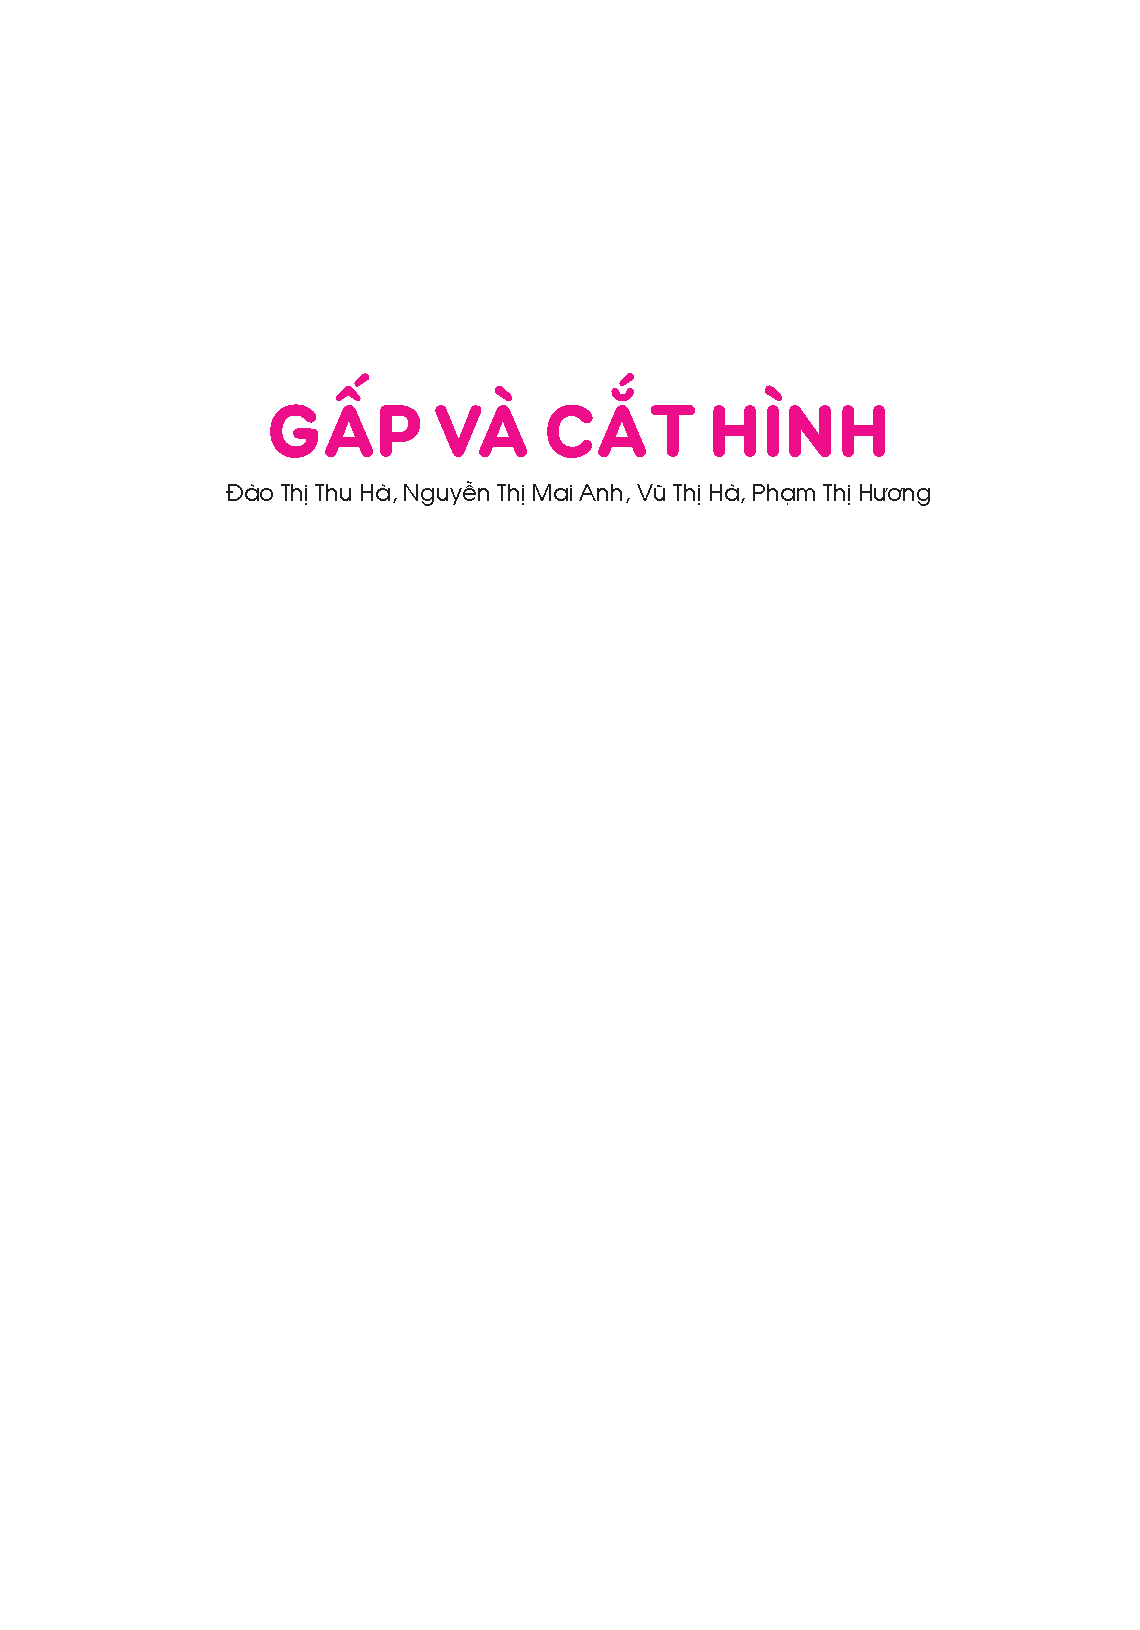
\includegraphics[scale=0.8]{../gapvacathinh/toancuabi}}} % %Image background
\centering
\endgroup
	
\vspace*{10pt}
	
Từ khi còn học mầm non, Bi  đã được làm quen với việc dùng kéo để cắt giấy, tạo ra nhiều hình khác nhau. Từ ngày biết về tính đối xứng, Bi đã áp dụng nó vào trò chơi cắt hình.
Nhiều hình tưởng phức tạp, nhưng mình sẽ cắt được nhanh hơn, nếu quan sát kỹ.
\vskip 0.1cm
Nào, chúng ta bắt đầu nhé.
\vskip 0.1cm
Bi gập đôi một tờ giấy lại và cắt bỏ một phần như hình vẽ dưới đây: 
	\begin{figure}[H]
		\centering
		\centering
		\vspace*{-10pt}
		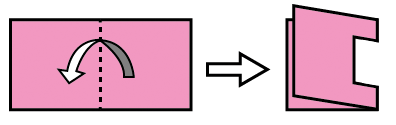
\includegraphics[scale=0.4]{cat-1}
		\vspace*{-10pt}
	\end{figure}
Em có biết khi mở tờ giấy ra, Bi nhận được hình nào trong những hình sau hay không?
\begin{figure}[H]
	\centering
	\captionsetup{labelformat=empty}
	\vspace*{-5pt}
	\captionsetup{justification=centering}
	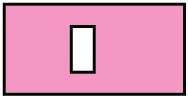
\includegraphics[width =0.16\textwidth]{cat-2a}\quad
	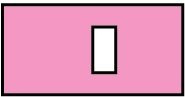
\includegraphics[width =0.16\textwidth]{cat-2b}\quad
	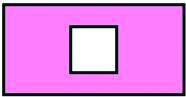
\includegraphics[width =0.16\textwidth]{cat-2c}\quad
	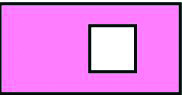
\includegraphics[width =0.16\textwidth]{cat-2d}\quad
	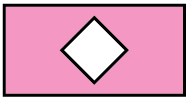
\includegraphics[width =0.16\textwidth]{cat-2e}
	\caption{\small\textit{(A) \hspace*{45pt} (B) \hspace*{45pt} (C) \hspace*{45pt} (D) \hspace*{45pt} (E)}}
	\vspace*{-5pt}
\end{figure}

Nếu còn nhớ về  tính đối xứng của hình vuông, các em sẽ thấy hình (\textit{C}) chính là đáp án đúng. Các em có thể dùng kéo và giấy để thử xem kết quả có đúng vậy không. Hãy cùng Bi thử với một hình phức tạp hơn nhé.
\vskip 0.1cm
\begin{multicols}{2}
	\textbf{\color{toancuabi}Câu hỏi $\pmb{1}$:} Bi gập đôi một tờ giấy lại và cắt bỏ một phần để phần còn lại là hình bên:
	
	\columnbreak
	\begin{figure}[H]
		\centering
		\captionsetup{labelformat=empty}
		\vspace*{-5pt}
		\captionsetup{justification=centering}
		
\includegraphics[width =0.2\textwidth]{cat-3}
		\vspace*{-10pt}
	\end{figure}
\end{multicols}
Hỏi khi mở tờ giấy ra, Bi đã nhận được hình nào trong các hình dưới đây (đường nét đứt là đường gập đôi)?
\begin{figure}[H]
	\centering
	\captionsetup{labelformat=empty}
	\vspace*{-5pt}
	\captionsetup{justification=centering}
	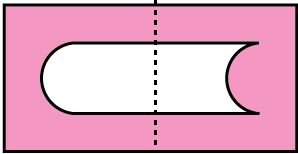
\includegraphics[width =0.2\textwidth]{cat-3a}\quad
	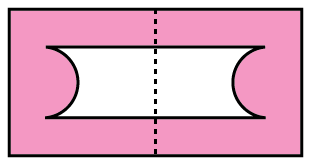
\includegraphics[width =0.2\textwidth]{cat-3b}\quad
	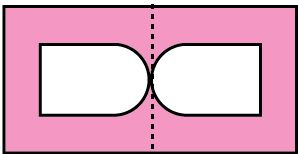
\includegraphics[width =0.2\textwidth]{cat-3c}\quad
	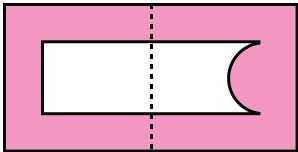
\includegraphics[width =0.2\textwidth]{cat-3d}
	\caption{\small\textit{(A) \hspace*{55pt} (B) \hspace*{55pt}(C) \hspace*{55pt} (D)}}
	\vspace*{-10pt}
\end{figure}
Từ đó, Bi thấy, nếu muốn cắt được một hình đối xứng, Bi có thể gập đôi tờ giấy lại để cắt. Vậy là Bi đến đố các bạn trong lớp.
\vskip 0.1cm
\textbf{\color{toancuabi}Câu hỏi $\pmb{2}$:} Bi gập đôi một tờ giấy lại và đố Ly cắt ra hình trái tim.
\begin{figure}[H]
	\centering
	\captionsetup{labelformat=empty}
	\vspace*{-5pt}
	\captionsetup{justification=centering}
	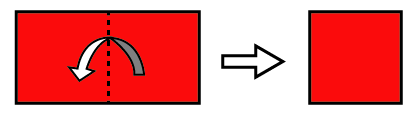
\includegraphics[width =0.65\textwidth]{cat-4}
	\vspace*{-10pt}
\end{figure}
Hỏi Ly cần phải cắt như thế nào để có hình trái tim ở trên?
\begin{figure}[H]
	\centering
	\captionsetup{labelformat=empty}
	\vspace*{-4pt}
	\captionsetup{justification=centering}
	
\includegraphics[width =0.1\textwidth]{cat-4a}
	\hfill
	
\includegraphics[width =0.1\textwidth]{cat-4b}
	\hfill
	
\includegraphics[width =0.1\textwidth]{cat-4c}
	\hfill
	
\includegraphics[width =0.1\textwidth]{cat-4d}
	\vspace*{-5pt}
	\caption{\small \it (A)\hspace*{75pt} (B)\hspace*{75pt} (C) \hspace*{75pt} (D)}
	\vspace*{-10pt}
\end{figure}
\begin{multicols}{2}
	Để cắt một hình vuông, ở trên, Bi đã gập đôi và cần ba nhát cắt (mỗi nhát ở đây được coi là một lần cắt thẳng). Tuy nhiên, với một lần gập đôi, và quan sát kĩ hình vuông, Bi chỉ cần hai nhát cắt để có được hình vuông: 
	
	\columnbreak
	\begin{figure}[H]
		\captionsetup{labelformat=empty}
		\vspace*{20pt}
		\centering
		\captionsetup{justification=raggedleft}
		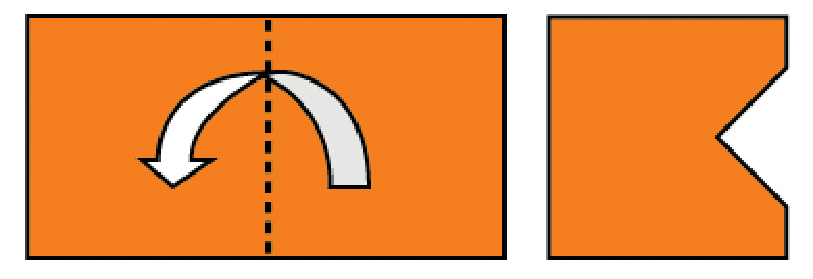
\includegraphics[width =0.44\textwidth]{cat-5}
		\vspace*{-5pt}
	\end{figure}
\end{multicols}
%\insertpic{195}{710}{.7}{../gapvacathinh/arrow}
%\insertpic{40}{700}{.35}{cat-4}
%\insertpic{228}{700}{.45}{cat-4them}
Em hãy thử suy nghĩ xem, với một lần gập đôi, liệu Bi có thể chỉ dùng một nhát cắt mà có  được hình vuông hay không? Với điều kiện khi cắt xong, ngoài hình vuông nhận được thì tờ giấy cũ vẫn còn liền nhau (không bị chia nhỏ).
\vskip 0.1cm
\begin{multicols}{2}
	\textbf{\color{toancuabi}Câu hỏi $\pmb{3}$:} Từ một miếng giấy, để cắt được đúng một chú bướm như hình dưới đây, em có thể gập đôi nhiều nhất mấy lần để cắt?
	
	\columnbreak
	\begin{figure}[H]
		\captionsetup{labelformat=empty}
		\vspace*{-5pt}
		\centering
		\captionsetup{justification=raggedleft}
		
\includegraphics[width =0.3\textwidth]{cat-6}
	\end{figure}
\end{multicols}

Sau một vài lần thử gập một lần, Bi chuyển sang gập tờ giấy hai lần để khám phá và tìm ra các câu đố mới cho các bạn trong lớp.
\vskip 0.1cm
Bi đã gập đôi tờ giấy hai lần như hình bên dưới. Sau đó, Bi cắt một góc của tờ giấy: 
\begin{figure}[H]
	\captionsetup{labelformat=empty}
	\vspace*{5pt}
	\centering
	\captionsetup{justification=raggedleft}
	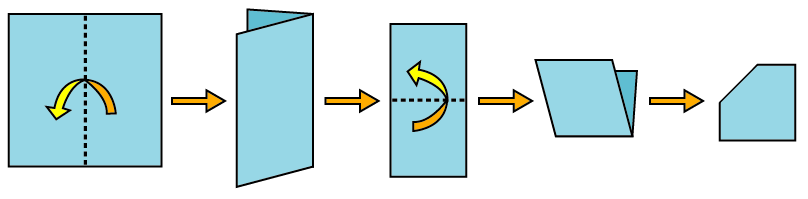
\includegraphics[width =0.85\textwidth]{cat-7a}
\end{figure}
\textbf{\color{toancuabi}a)} Khi mở tờ giấy ra một lần, Bi thu được hình nào dưới đây?
\begin{figure}[H]
	\centering
	\captionsetup{labelformat=empty}
	\vspace*{-4pt}
	\captionsetup{justification=centering}
	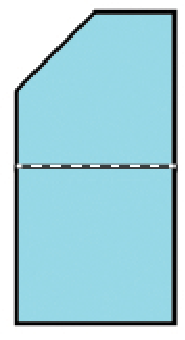
\includegraphics[width =0.08\textwidth]{cat-8a}
	\hfill
	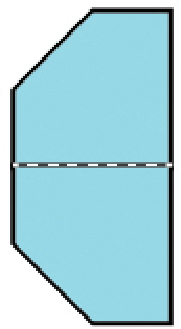
\includegraphics[width =0.08\textwidth]{cat-8b}
	\hfill
	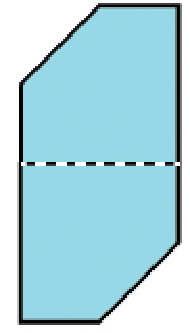
\includegraphics[width =0.08\textwidth]{cat-8c}
	\hfill
	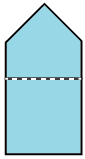
\includegraphics[width =0.08\textwidth]{cat-8d}
	\hfill
	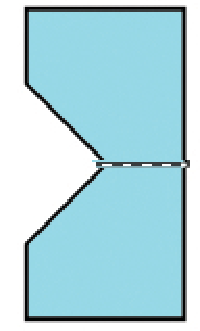
\includegraphics[width =0.08\textwidth]{cat-8e}	
	\caption{\small \it (A)\hfill (B) \hfill (C) \hfill (D) \hfill (E)}
	\vspace*{-10pt}
\end{figure}

\textbf{\color{toancuabi}b)} Khi mở tờ giấy ra hai lần, Bi thu được hình nào dưới đây?
\begin{figure}[H]
	\centering
	\captionsetup{labelformat=empty}
	\vspace*{-5pt}
	\captionsetup{justification=centering}
	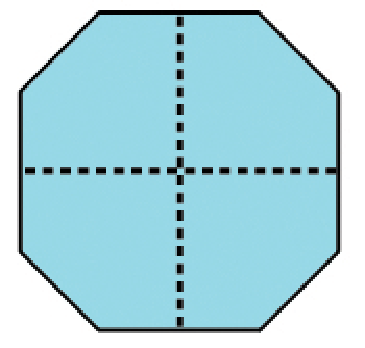
\includegraphics[width =0.19\textwidth]{cat-9a}
	\hfill
	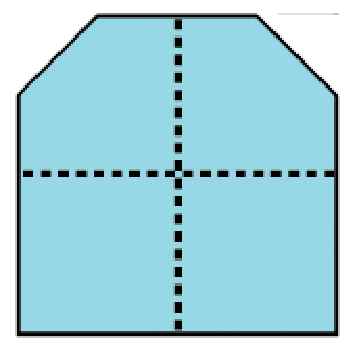
\includegraphics[width =0.19\textwidth]{cat-9b}
	\hfill
	
\includegraphics[width =0.19\textwidth]{cat-9c}
	\hfill
	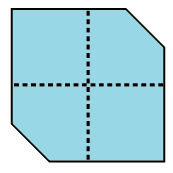
\includegraphics[width =0.19\textwidth]{cat-9d}
	\caption{\small \it (A) \hfill (B) \hfill (C) \hfill (D) \hfill (E)}
\end{figure}
Các em có tìm được câu trả lời không? Mình có thể làm từ từ từng bước đấy. Với câu a), đường đứt ở giữa là vết gập khi mở lần đầu tiên. Và dựa vào tính đối xứng, đáp án của câu a) chính là hình ($B$).
\vskip 0.1cm
Sau khi mở ra lần hai, đường đứt nằm dọc chính là vết gập khi mở lần hai. Đáp án của câu b) chính là hình (\textit{A}).
\vskip 0.1cm
Hình vuông có bốn trục đối xứng. Khi gập đôi một lần, Bi thấy để cắt rời hình vuông ra khỏi một tờ giấy, Bi cần cắt ba nhát hoặc hai nhát. Bây giờ, với hai lần gập giấy, liệu số nhát cắt cần thiết có ít đi hay không?
\vskip 0.1cm
\textbf{\color{toancuabi}Câu hỏi $\pmb{4}$:} Bi gập đôi tờ giấy hai lần như hình bên dưới. 
\begin{figure}[H]
	\captionsetup{labelformat=empty}
	\vspace*{-5pt}
	\centering
	\captionsetup{justification=raggedleft}
	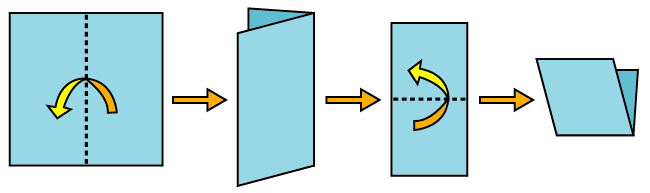
\includegraphics[width =0.7\textwidth]{cat-10}
	\vspace*{-10pt}
\end{figure}
Sau đó, Bi đã đố My chỉ bằng một nhát cắt, hãy cắt ra một hình vuông. Hỏi My nên cắt như thế nào?
\begin{figure}[H]
	\vspace*{-5pt}
	\centering
	\captionsetup{labelformat=empty}
	\captionsetup{justification=centering}
	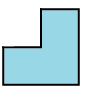
\includegraphics[width =0.2\textwidth]{cat-10a}
	\hfill
	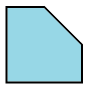
\includegraphics[width =0.2\textwidth]{cat-10b}
	\hfill
	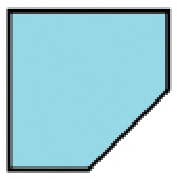
\includegraphics[width =0.2\textwidth]{cat-10c}
	\hfill
	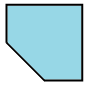
\includegraphics[width =0.2\textwidth]{cat-10d}	
	\vspace*{-5pt}
	\caption{\small \it (A)\hspace*{40pt} (B)\hspace*{65pt} (C) \hspace*{40pt} (D)}
	\vspace*{-10pt}
\end{figure}
\begin{multicols}{2}
	Bi biết là các bạn gái rất thích cắt hoa. Thế là Bi đố Ly cắt bông hoa bốn cánh.
	
	\columnbreak
	\begin{figure}[H]
		\vspace*{-5pt}
		\captionsetup{labelformat=empty}
		\centering
		\captionsetup{justification=raggedleft}
		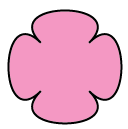
\includegraphics[width =0.2\textwidth]{cat-11}
		\vspace*{-10pt}
	\end{figure}
\end{multicols}
\textbf{\color{toancuabi}Câu hỏi $\pmb{5}$:} Bi gập đôi tờ giấy hai lần như hình bên dưới.
\begin{figure}[H]
	\vspace*{-5pt}
	\captionsetup{labelformat=empty}
	\centering
	\captionsetup{justification=raggedleft}
	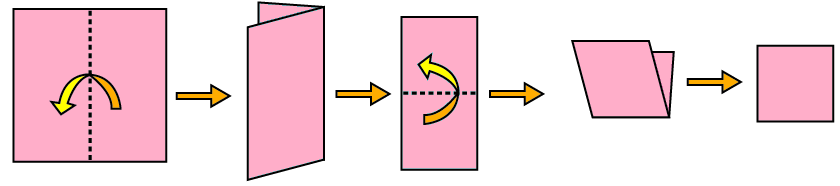
\includegraphics[width =1\textwidth]{cat-12}
	\vspace*{-10pt}
\end{figure}
Ly nên cắt tờ giấy (đã được gập) như thế nào để có được bông hoa bốn cánh ở trên?
\begin{figure}[H]
	\centering
	\captionsetup{labelformat=empty}
	\vspace*{-5pt}
	\captionsetup{justification=centering}
	
\includegraphics[width =0.2\textwidth]{cat-13a}
	\hfill
	
\includegraphics[width =0.2\textwidth]{cat-13b}
	\hfill
	
\includegraphics[width =0.2\textwidth]{cat-13c}
	\hfill
	
\includegraphics[width =0.2\textwidth]{cat-13d}	
	\vspace*{-5pt}
	\caption{\small \it (A)\hspace*{40pt} (B)\hspace*{65pt} (C) \hspace*{40pt} (D)}
	\vspace*{-10pt}
\end{figure}
Ly đã trả lời đúng câu đố của Bi đấy. Nhưng sau đó, Ly thấy rằng, nếu gập thêm một lần nữa thì sẽ cắt bông hoa còn nhanh hơn cơ.
\vskip0.25cm
\textbf{\color{toancuabi}Câu hỏi $\pmb{6}$:} Từ mảnh giấy hình tròn, Ly gập đôi mảnh giấy ba lần như hình bên dưới: 
\begin{figure}[H]
	\vspace*{-10pt}
	\captionsetup{labelformat=empty}
	\centering
	\captionsetup{justification=raggedleft}
	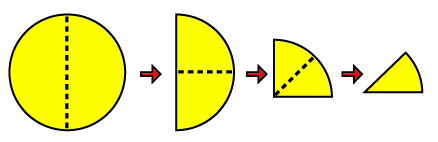
\includegraphics[width =0.85\textwidth]{cat-14}
\end{figure}	
Ly  đã cắt như thế nào để có được hình bông hoa bốn cánh?
\begin{figure}[H]
	\centering
	\captionsetup{labelformat=empty}
	\vspace*{-10pt}
	\captionsetup{justification=centering}
	
\includegraphics[width =0.2\textwidth]{cat-15a}
	\hfill
	
\includegraphics[width =0.2\textwidth]{cat-15b}
	\hfill
	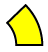
\includegraphics[width =0.2\textwidth]{cat-15c}
	\hfill
	
\includegraphics[width =0.2\textwidth]{cat-15d}	
	\caption{\small \it (A)\hspace*{40pt} (B)\hspace*{65pt} (C) \hspace*{40pt} (D)}
	\vspace*{-10pt}
\end{figure}
Từ đó, em hãy suy nghĩ xem, nếu cắt bông hoa sáu cánh, tám cánh, thì làm như thế nào sẽ cắt được bông hoa có các cánh đều nhất và nhanh nhất nhé. Và nếu muốn cắt hình lục giác đều, ngũ giác đều, thì nên làm như thế nào? 
\begin{figure}[H]
	\centering
	\captionsetup{labelformat=empty}
%	\vspace*{-5pt}
	\captionsetup{justification=centering}
	
\includegraphics[width =0.2\textwidth]{cat-16a}
	\hfill
	
\includegraphics[width =0.2\textwidth]{cat-16b}
	\hfill
	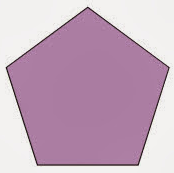
\includegraphics[width =0.2\textwidth]{cat-16c}
	\hfill
	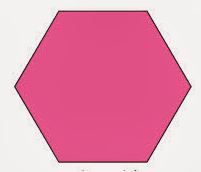
\includegraphics[width =0.2\textwidth]{cat-16d}	
	\vspace*{-5pt}
\end{figure}
Bây giờ, mình hãy cùng xem khi cắt hình phức tạp hơn một chút thì hình nhận được sẽ thế nào.
\vskip0.3cm
\textbf{\color{toancuabi}Câu hỏi $\pmb{7}$:} Bi đã gập và cắt một mảnh giấy hình tròn như mô tả dưới đây:
\begin{figure}[H]
	\vspace*{-5pt}	
	\captionsetup{labelformat=empty}
	\centering
	\captionsetup{justification=raggedleft}
	\includegraphics[width =1\textwidth]{cat-17}
	\vspace*{-10pt}
\end{figure}
Hỏi khi mở tờ giấy ra, bạn ấy sẽ thu được hình nào (bạn ấy giữ lại phần ở giữa)?
\begin{figure}[H]
	\centering
	\captionsetup{labelformat=empty}
	\vspace*{-5pt}
	\captionsetup{justification=centering}
	\includegraphics[width =0.2\textwidth]{cat-17a}
	\hfill
	\includegraphics[width =0.2\textwidth]{cat-17b}
	\hfill
	\includegraphics[width =0.2\textwidth]{cat-17c}
	\hfill
	\includegraphics[width =0.2\textwidth]{cat-17d}
	\caption{\small \it (A)\hspace*{40pt} (B)\hspace*{65pt} (C) \hspace*{40pt} (D)}	
	\vspace*{-10pt}
\end{figure}
\begin{multicols}{2}
	Hãy cùng làm những hình trang trí khác nhau từ cách cắt  hình mà chúng mình  đã khám phá cùng Bi ngày hôm nay nhé.
	\begin{figure}[H]
		\vspace*{-5pt}	
		\captionsetup{labelformat=empty}
		\centering
		\captionsetup{justification=raggedleft}
		\includegraphics[width =0.3\textwidth]{cat-18}
		\vspace*{-10pt}
	\end{figure}
\end{multicols}
	\newpage
\graphicspath{{../choicungbi/tangram/}}
\blfootnote{$^1$Công ty Cổ phần phát triển giáo dục POMATH.}
	\begingroup
	\AddToShipoutPicture*{\put(42,595){\includegraphics[scale=0.7]{../tangram/toancuaBi_2-tieude}}} % %Image background
	\centering
	\endgroup	
	
\vspace*{25pt}

	Mở đầu cho bài viết trong số này, Bi xin mời các bạn quan sát các hình ảnh sau:
	\begin{figure}[H]
		\vspace*{-5pt}
		\centering
		\captionsetup{labelformat=empty}
		\begin{subfigure}{.45\textwidth}
		\captionsetup{labelformat=empty}
		\centering
		\includegraphics[width=.5\linewidth]{image1}
		\caption{\small \it Hình $1$}
		\end{subfigure}
		\begin{subfigure}{.45\textwidth}
		\captionsetup{labelformat=empty}
		\centering
		\includegraphics[width=.5\linewidth]{image2}
		\caption{\small \it Hình $2$}
	\end{subfigure}
	\vspace*{-10pt}
\end{figure}	
	Các bạn tưởng tượng ra hình gì?
	\vskip 0.1cm
	Chắc là các bạn sẽ tưởng tượng ra hình trái tim, hình con thuyền, cũng có bạn lại nghĩ đây là hình con chim. Nhưng các bạn có tìm ra được đặc điểm chung của hai hình trên không?
	\begin{multicols}{2}
		Bi xin bật mí với các bạn, hai hình này có cùng diện tích đấy! Hay chính xác hơn, cả hai hình này đều được ghép từ $7$ mảnh ghép. Xem này:
		\begin{figure}[H]
			\vspace*{5pt}
			\centering
			\captionsetup{labelformat=empty}
			\includegraphics[width=.4\linewidth]{imame3}\includegraphics[width=.4\linewidth]{image4}
			\caption{\small \it Hình $3$\hspace*{30pt} Hình $4$}
			\vspace*{-10pt}
		\end{figure}
	\end{multicols}
	Nếu bạn nào còn băn khoăn vì sao hai hình khác nhau nhiều như thế mà diện tích lại bằng nhau thì Bi xin mời các bạn xem tiếp $7$ mảnh ghép này Biến hóa như thế nào nhé!
	\begin{multicols}{2}
		Đến bây giờ thì các bạn đều hiểu rồi chứ? Chúng ta đều có thể cắt ghép hai hình ban đầu thành $7$ mảnh ghép, rồi dùng $7$ mảnh ghép đó ghép lại thành một hình vuông. Vì vậy, chúng có diện tích bằng nhau. Quả là rất thú vị phải không?
		\begin{figure}[H]
			\vspace*{5pt}	
			\captionsetup{labelformat=empty}
			\centering
			\captionsetup{justification=raggedleft}
			\includegraphics[width =0.3\textwidth]{image5}
			\caption{\small\it Hình $5$.}
			\vspace*{-10pt}
		\end{figure}
	\end{multicols}
	Và các bạn Biết không, những gì Bi vừa giới thiệu trên đây đều xuất phát từ một trò chơi mang tên gọi: TANGRAM.
	
	\vspace*{-5pt}
	\begin{multicols}{2}
		Tangram là một món đồ chơi xuất hiện rất lâu đời ở Trung Quốc. Theo tiếng Trung Quốc, ``Tangram" nghĩa là ``$7$ mảnh ghép thông minh", gồm $7$ mảnh ghép (Gọi là ``tans") được cắt ra từ một hình vuông lớn, bao gồm: $1$ hình vuông, $1$ hình bình hành, $2$ tam giác vuông cân nhỏ, $1$ tam giác vuông cân vừa và $2$ tam giác vuông cân lớn.
		\vskip 0.1cm
		\textit{\small (Tam giác vuông cân là tam giác có một góc vuông và có $2$ cạnh bằng nhau)}
		\begin{figure}[H]
			\vspace*{-20pt}	
			\captionsetup{labelformat=empty}
			\centering
			\captionsetup{justification=raggedleft}
			\includegraphics[width =0.2\textwidth]{image6}
			\caption{\small\it Hình $6$.}
%			\vspace*{5pt}
		\end{figure}
	\end{multicols}
	\vspace*{-5pt}
	Luật chơi của Tangram rất đơn giản: Dùng đúng $7$ mảnh ghép của trò chơi để xếp ra các hình có nghĩa khác nhau, đảm bảo các mảnh ghép không trùng lên nhau.
	\vspace*{-5pt}
	\begin{multicols}{2}
		\begin{figure}[H]
			\vspace*{5pt}	
			\captionsetup{labelformat=empty}
			\centering
			\captionsetup{justification=raggedleft}
			\includegraphics[width =0.2\textwidth]{image7}
			\caption{\small\it Hình $7$.}
			\vspace*{-10pt}
		\end{figure}
		Đầu thế kỉ $19$, Tangram đã vượt ra khỏi Biên giới Trung Quốc thông qua những con tàu buôn của những nhà thương gia phương Tây. \linebreak Tangram đặt chân đến Mỹ, các nước Châu Âu và nhanh chóng tạo ra cơn sốt về một trò chơi thú vị nhưng cũng đầy thách thức. Cũng từ đó, Biến thể của
		Tangram xuất hiện ngày càng nhiều, không còn giữ nguyên khuôn hình vuông như ban đầu nữa. Vì vậy, số lượng hình ghép được tăng lên gấp nhiều lần và đương nhiên, những hình ``cực khó" cũng xuất hiện với mật độ ngày càng lớn.
		\begin{figure}[H]
			\vspace*{-10pt}	
			\captionsetup{labelformat=empty}
			\centering
			\captionsetup{justification=raggedleft}
			\includegraphics[width =0.2\textwidth]{image8}
			\caption{\small\it Hình $8$.}
%			\vspace*{-10pt}
		\end{figure}
		Nhìn các hình ảnh trên, các bạn đã thấy hấp dẫn chưa? Nhưng điều hấp dẫn hơn sẽ nằm ngay sau đây: Bi sẽ hướng dẫn các bạn tự tạo ra bộ trò chơi này mà không cần đi mua ở đâu cả. Chúng ta bắt đầu nhé!
	\vskip 0.1cm
	\textbf{Chuẩn bị và thực hiện}
	\vskip 0.1cm
	\textbf{* Chuẩn bị:}
	\vskip 0.1cm
	-- $1$ tờ giấy bìa hình vuông kích thước $8$cm $\times$ $8$cm.
	\vskip 0.1cm
	-- Thước kẻ, bút chì, kéo, màu sáp.
	\vskip 0.1cm
	\textbf{* Thực hiện:}
	\vskip 0.1cm
	\textit{Bước $1$:} Kí hiệu tờ bìa hình vuông là $ABCD$ (hình vẽ).
	\vskip 0.1cm
	\textit{Bước $2$:} 
	\vskip0.05cm
	+/ Trên cạnh $AB$ lấy điểm $E$ sao cho $AE = EB = 4cm$.
	\vskip 0.1cm
	+/ Trên cạnh $AD$ lấy điểm $F$ sao cho $AF = FD = 4cm$.
	\vskip 0.1cm
	+/ Trên đoạn $EF$ lấy điểm $G$ sao cho $GE= GF$.
	\vskip 0.1cm
	+ Trên đoạn $BD$ lấy các điểm $H, O, I$ sao cho $DH = HO = OI = IB$.
	\vskip 0.1cm
	\textit{Bước $3$:} Nối $G$ với $O, G$ với $H, O$ với $C, E$ với $I$.
	\begin{figure}[H]
		\vspace*{-10pt}
		\centering
		\includegraphics[scale=0.2]{image9}
		\vspace*{-10pt}
	\end{figure}
	\textit{Bước $4$:} Dùng kéo cắt thành $7$ mảnh rồi dùng màu sáp tô màu theo ý thích.
	\end{multicols}
	Chúng ta đã tạo ra được một bộ Tangram rồi, thật là dễ đúng không? Các bạn hãy dùng bộ Tangram vừa tạo để ghép các hình phía trên nhé!
	\vskip 0.1cm
	Nhưng Bi luôn có một câu hỏi: ``Liệu chúng ta có thể tự tạo ra cho mình một bộ Tangram?". Không Biết có bạn nhỏ nào cũng đặt câu hỏi giống như Bi không?
	\vskip 0.1cm
	Vậy thì chúng ta thử cùng nhau nghiên cứu các bộ Tangram xem phát hiện ra được điều lí thú gì nhé!
	\begin{figure}[H]
	\centering
	\vspace*{-10pt}
	\includegraphics[scale=0.2]{image10}\quad
	\includegraphics[scale=0.2]{image11}\quad
	\includegraphics[scale=0.2]{image12}
	\end{figure}
	\textit{Bi nhận thấy, hình vuông $OIEG$ có thể chia thành $2$ tam giác vuông nhỏ. Lúc này, ta có $2$ hình  bình hành bằng nhau là $DHGF$ và $HOEG$}
	\vskip 0.1cm
	\textit{Vì vậy, hình bình hành $DHGF$ cũng có thể chia thành $2$ tam giác vuông nhỏ như hình bình hành $HOEG$.
	\vskip 0.1cm
	Liệu các mảnh còn lại có chia được thành các tam giác vuông nhỏ như trên?}
	\vskip 0.1cm
	\textit{Câu trả lời là có.
	\vskip 0.1cm
	Tất cả $7$ mảnh của bộ Tangram này đều được tạo ra từ $1$ hay nhiều tam giác vuông cân cùng kích thước.}
	\begin{multicols}{2}
	Quả là bất ngờ đúng không các bạn? Như vậy, chúng ta chỉ cần sử dụng các tam giác vuông cân giống nhau là có thể tạo ra một bộ Tangram mới rồi! Ví dụ, Bi sẽ chọn cách ghép các tam giác vuông như sau:
	\vskip 0.1cm
		Bây giờ, các bạn hãy tạo một bộ Tangram giống của Bi và ghép thành các hình sau. Đừng quên tưởng tượng xem mỗi hình ảnh thể hiện sự vật gì nhé!
		\begin{figure}[H]
			\vspace*{-15pt}
			\centering
			\captionsetup{labelformat=empty}
			\includegraphics[width=0.25\textwidth]{image13}
			\caption{\small \it Hình $9$ -- Bộ Tangram gồm $4$ tam giác vuông cân, $1$ hình vuông, $1$ hình thang vuông, $1$ hình thang cân}
			\vspace*{-5pt}
		\end{figure}
	\end{multicols}
	\begin{figure}[H]
		\vspace*{-5pt}
		\centering
		\includegraphics[width=0.65\textwidth]{cat-10}
		\vspace*{-5pt}
	\end{figure}



	%\pagecolor{lightgray} 
\newpage
\graphicspath{{../choicungbi/boxephinh/}}
\begingroup
\AddToShipoutPicture*{\put(70,605){\includegraphics[scale=0.84]{../boxephinh/tieude.pdf}}} 
\centering
\endgroup
%
\vspace*{15pt}
	\begin{multicols}{2}
		Cuối tuần, chị My cầm đến một bộ xếp hình nam châm để chơi cùng Bi. Khỏi phải nói là cậu bé Bi tò mò đã hứng khởi đến như thế nào. Bi đã xếp được bao nhiêu là hình rất chi là thú vị nhé.
		\vskip 0.1cm
		Bộ xếp hình nam châm có các thanh màu đỏ,  xanh hoặc đen và các viên bi tròn để có thể gắn các thanh lại với nhau.
		\vskip 0.1cm
		Các bé hãy cùng Bi khám phá xem chúng mình có thể vui học được gì qua bộ nam châm này nhé.
		\vskip 0.1cm
		Kim tự tháp tam giác (chóp tam giác) là hình đầu tiên mà Bi xếp được đó. Các bạn hãy quan sát để trả lời câu hỏi sau nhé.
		\begin{figure}[H]
			\centering
			\vspace*{-5pt}
			\captionsetup{labelformat= empty, justification=centering}
			\includegraphics[width=0.25\textwidth]{1}
			\caption{\small\textit{Hình $1$}}
			\vspace*{-10pt}
		\end{figure}
		\begin{figure}[H]
			\centering
%			\vspace*{5pt}
			\captionsetup{labelformat= empty, justification=centering}
			\includegraphics[width=0.23\textwidth]{2}
			\caption{\small\textit{Hình $2$}}
			\vspace*{-5pt}
		\end{figure}
	\end{multicols}
	
	\textbf{Câu hỏi $\pmb{1}$:} \textit{a. Nhìn vào hình vẽ và cho biết Bi đã dùng bao nhiêu viên bi và bao nhiêu thanh màu đen để ghép được Hình $2$?
	\vskip 0.1cm
	b. Có tất cả bao nhiêu tam giác có các cạnh là các thanh màu đen? }
	\begin{multicols}{2}
		Quá là đơn giản nhỉ? Hình kim tự tháp có đáy là hình tam giác này có $4$ đỉnh và $6$ cạnh, nên để ghép hình đó, Bi đã dùng $4$ viên bi và $6$ thanh màu đen.
		\begin{figure}[H]
			\centering
			\vspace*{5pt}
			\captionsetup{labelformat= empty, justification=centering}
			\includegraphics[width=0.35\textwidth]{3}
			\caption{\small\textit{Hình $3$ -- Kim tự tháp tam giác}}
			\vspace*{-5pt}
		\end{figure}
	\end{multicols}	
	Bây giờ, để đếm số tam giác, đó chính là số mặt của kim tự tháp, nên chúng mình dễ dàng biết được là trong hình có $4$ tam giác có cạnh là các thanh màu đen, ứng với $4$ mặt của hình kim tự tháp.
	\vskip 0.1cm
	Hình tiếp theo mà Bi đố các bé không còn đơn giản như thế nữa đâu, chúng mình cần phải quan sát kỹ hơn đó.
	\vspace*{-5pt}
	\begin{multicols}{2}
		\begin{figure}[H]
			\centering
			\vspace*{5pt}
			\captionsetup{labelformat= empty, justification=centering} \includegraphics[width=0.35\textwidth]{4}
			\caption{\small\textit{Hình $4$}}
			\vspace*{-5pt}
		\end{figure}
		Trong Hình $4$ có hai góc nhìn khác nhau của cùng một khối hình. Nhìn có vẻ khó quan sát hơn rồi ấy nhỉ? Chúng mình cùng quan sát và tìm cách trả lời câu hỏi sau nhé.
	\end{multicols}
	\vspace*{-5pt}
	\textbf{Câu hỏi $\pmb{2}$:} \textit{Để xếp Hình $4$, Bi đã dùng tất cả bao nhiêu viên bi và bao nhiêu thanh đen?}
	\vspace*{-5pt}
	\begin{multicols}{2}
		Để trả lời câu hỏi này, Bi cũng rất suy nghĩ đấy. Dĩ nhiên là nếu phá bỏ khối hình và ngồi đếm từ từ thì quá đơn giản rồi. Nhưng đó đâu còn thú vị và thử thách nữa. Sau một hồi quan sát, thì Bi đã ló ra một ý tưởng để đếm số viên bi, đó là hãy đếm theo từng tầng. Bi đã chia khối hình thành ba tầng như Hình $5$.
		\begin{figure}[H]
			\centering
			\vspace*{-5pt}
			\captionsetup{labelformat= empty, justification=centering} \includegraphics[width=0.32\textwidth]{5}
			
			\vspace*{-10pt}
			\caption{\small\textit{Hình $5$}}
			\vspace*{-5pt}
		\end{figure}
	\end{multicols}
	Bây giờ thì các bé đã thấy câu trả lời chưa? Từ  Hình $6$, chúng mình dễ dàng đếm được tầng $3$ thì chỉ có $1$ viên bi, tầng $2$ thì có $1+2 = 3$ viên bi, còn tầng $1$ thì có nhiều nhất là $1 + 2 + 3 = 6$ viên bi. Thế nên tổng cộng Bi đã dùng:
	$1 + 3 + 6 = 10 \text{ (viên bi)}.$
	\begin{multicols}{2}
		\begin{figure}[H]
			\centering
			\vspace*{15pt}
			\captionsetup{labelformat= empty, justification=centering} \includegraphics[width=0.475\textwidth]{6}
			\caption{\small\textit{Hình $6$}}
			\vspace*{-5pt}
		\end{figure}
		Nhưng còn để đếm số thanh đen thì không chỉ đơn giản như vậy nữa, đã phức tạp hơn rất nhiều rồi đấy. Có rất nhiều cách để đếm khác nhau, nhưng để Bi giới thiệu với các bé hai cách Bi đã tìm ra nhé.
	\end{multicols}
	\vskip 0.1cm
	\textbf{Cách $1$:} Khối hình này cũng là một kim tự tháp, nhưng mà là kim tự tháp to hơn Hình $2$. Khối hình này cũng có $6$ cạnh, mỗi cạnh cần $2$  thanh để ghép thành, ví dụ như phần được tô màu xanh trong Hình $7$. Vậy để làm thành các cạnh của khối kim tự tháp, Bi đã dùng:
	$ 2\times 6 = 12 \text{ (thanh đen)}.$
	\begin{multicols}{2}
		\begin{figure}[H]
			\centering
			\vspace*{5pt}
			\captionsetup{labelformat= empty, justification=centering} \includegraphics[width=0.3\textwidth]{7}
			\caption{\small\textit{Hình $7$}}
			\vspace*{-10pt}
		\end{figure}
		Nhưng như thế chưa đủ số thanh. Khối hình này có $4$ mặt, và mỗi mặt thì đều như tầng $1$ của Hình $6$. Ngoài các thanh đã dùng để xếp cạnh của kim tự tháp, mỗi mặt còn cần thêm $3$ thanh được tô màu đỏ để xếp nữa. Vậy tức là Bi cần dùng thêm $3 \times 4 = 12$ thanh màu đen để xếp các phần ở các mặt của kim tự tháp trong Hình $4$ mà không phải là cạnh.
	\end{multicols}
	\vskip 0.1cm
	Các bé thử quan sát xem vậy là đã đủ hết chưa nhỉ? Bi sẽ bật mí cho các bé rằng đã đủ hết số  thanh cần dùng rồi đó. Để xếp được hình ba tầng, Bi đã dùng tổng cộng:
	$ 12 + 12 = 24 \text{ (thanh đen)}.$
	\vskip 0.1cm
	\textbf{Cách $2$:} Những tưởng tìm được cách đếm này là đã đủ để hài lòng, thế nhưng Bi đã tìm ra cách đếm khác nữa đấy, vì cách đếm thứ hai này giúp Bi dễ dàng đếm với những hình nhiều tầng hơn nữa cơ.
	\vskip 0.1cm
	Chúng mình cùng quan sát lại khối hình và sẽ nhìn thấy hình $3$ tầng thật ra có rất nhiều hình kim tự tháp nhỏ bên trong đấy. Nhìn vào hình $8$, mình chia ra hình kim tự tháp đầu tiên có một mặt đáy là tầng $2$ (các cạnh màu đỏ), và có $3$ kim tự tháp có các mặt đáy là các tam giác thuộc tầng $3$. Và khối hình đã được chia ra làm $4$ kim tự tháp, các cạnh màu đen đều được xuất hiện đầy đủ trong cách chia này. Vậy nên ta có cách để tính số thanh đã dùng để xếp là: 
	$$4 \times 6 = 24 \text{ (thanh đen)}.$$	
	\begin{multicols}{2}
		Hình bên trái tô màu hình kim tự tháp trên cùng $- 4$ cạnh màu đỏ. Hình bên phải tô màu $3$ cái kim tự tháp bên dưới, mỗi cái một màu.
		\vskip 0.1cm
		Bi đã thử lại bằng cách dỡ bỏ khối hình ra và đếm lại rồi đấy, thật là chính xác luôn. Các bé cũng có thể thử bằng cách dùng các thanh gỗ và tre để thay thế cho các thanh đen, và dùng kẹo dẻo hoặc đất nặn thay cho các viên bi.
		\begin{center}
			\centering
			\vspace*{-10pt}
			\captionsetup{labelformat= empty, justification=centering} \includegraphics[width=0.2\textwidth]{8}\quad
			\includegraphics[width=0.2\textwidth]{8a}
			\textit{\small Hình $8$}
%			\vspace*{-5pt}
		\end{center}
	\begin{figure}[H]
		\centering
		\vspace*{-15pt}
		\captionsetup{labelformat= empty, justification=centering} \includegraphics[width=0.42\textwidth]{9}
		\caption{\small\textit{Hình $9$}}
		\vspace*{-5pt}
	\end{figure}
	\end{multicols}
	\vspace*{-5pt}
	Bây giờ, các bé hãy cùng thử sức với một câu hỏi khó hơn nhé.
	\vskip 0.1cm
	\textbf{Câu hỏi $\pmb{3}$:} \textit{Trong Hình $4$, có tất cả bao nhiêu tam giác có các cạnh là các thanh đen, trong đó mỗi cạnh là một thanh đen?}
%	\vspace*{-5pt}
	\vskip 0.1cm
%	\begin{multicols}{2}
	\begin{wrapfigure}{r}{0.25\textwidth}
		\centering
		\vspace*{-10pt}
		\captionsetup{labelformat= empty, justification=centering} \includegraphics[width=0.22\textwidth]{10}
		\caption{\small\textit{Hình $10$}}
		\vspace*{-15pt}
	\end{wrapfigure}
	Ngày càng phức tạp nhỉ? Để tính số tam giác, đầu tiên thì Bi quan sát $4$ mặt của khối hình. Mỗi mặt sẽ có $4$ hình tam giác nhỏ:
	\vskip 0.1cm
	Vậy là ở mặt ngoài của hình kim tự tháp, chúng mình có tổng cộng:
	\vskip 0.1cm
	\hspace*{35pt}{$4 \times 4 = 16 \text{ (tam giác cạnh $1$)}.$}
	\vskip 0.1cm
	\vspace*{5pt}
	Nhưng như vậy đã đủ chưa nhỉ? Mình dễ lầm tưởng là hết rồi, nhưng sau khi quan sát rất kỹ thì Bi nhìn thấy còn các hình khác nữa cơ.
	\vskip 0.1cm
	\begin{wrapfigure}{l}{0.25\textwidth}
		\centering
		\vspace*{-15pt}
		\captionsetup{labelformat= empty, justification=centering} \includegraphics[width=0.23\textwidth]{11}
		\vspace*{-5pt}
		\caption{\small\textit{Hình $11$}}
		\vspace*{-20pt}
	\end{wrapfigure}
	\vspace*{-1pt}
	Các bé hãy nhìn lại Hình $5$, chúng mình sẽ thấy tầng $2$ chính là một tam giác cạnh $1$. Vấn đề là có bao nhiêu tam giác như vậy nhỉ? Có $4$ mặt của kim tự tháp và tương ứng sẽ có $4$ tam giác kiểu tam giác ở tầng $2$. Thế là chúng mình có thêm $4$ tam giác nữa.
	\vskip 0.15cm
	Vậy là cuối cùng, Bi đã đếm được có tất cả $20$ tam giác cạnh $1$ đấy.
	\vskip 0.1cm
	\textbf{Câu hỏi $\pmb{4}$:} \textit{Trong Hình $4$, có tất cả bao nhiêu tam giác có các cạnh là các thanh đen, tính cả các tam giác “to”, tức là có cạnh nhiều hơn một thanh đen?}
	\vspace*{-5pt}
	\begin{multicols}{2}
		Để tìm được đáp án của câu này sau khi đã biết câu $3$, thì vấn đề đơn giản hơn nhiều. Trong Hình $4$, chỉ có các tam giác có cạnh bằng $1$  thanh đen hoặc tam giác có cạnh bằng $2$ thanh đen mà thôi. Số tam giác có cạnh bằng $2$ thanh đen dễ đếm hơn rất nhiều, mỗi mặt có đúng một tam giác như vậy, nên có tất cả $4$ tam giác có cạnh bằng $2$ thanh đen.
		\begin{figure}[H]
			\centering
			\vspace*{-5pt}
			\captionsetup{labelformat= empty, justification=centering} \includegraphics[width=0.3\textwidth]{12}
			\caption{\small\textit{Hình $12$}}
			\vspace*{-5pt}
		\end{figure}
	\end{multicols}
	Vậy là cuối cùng chúng mình đã tính được tổng số tam giác rồi đó, có $24$ tam giác các cỡ.
	\vskip 0.1cm
	Bây giờ, các bé hãy cùng thử sức với các câu hỏi tiếp theo nhé, khó hơn một chút đấy.
	\begin{multicols}{2}
	\textbf{Câu hỏi $\pmb{5}$:} \textit{a. Để xếp Hình $13$, Bi đã dùng tất cả bao nhiêu viên bi và bao nhiêu thanh đen? 
	\vskip 0.1cm
	b. Trong Hình $13$, có tất cả bao nhiêu tam giác có các cạnh là các thanh đen, tính cả các tam giác “to”, tức là có cạnh nhiều hơn một thanh đen?}
	\begin{figure}[H]
		\centering
		\vspace*{5pt}
		\captionsetup{labelformat= empty, justification=centering} \includegraphics[width=0.2\textwidth]{13}
		\quad
		\includegraphics[width=0.2\textwidth]{13a}
		\caption{\small\textit{Hình $13$}}
		\vspace*{-5pt}
	\end{figure}
	\end{multicols}








	\newpage
\graphicspath{ {../choicungbi/domino1/} }
\begingroup
\AddToShipoutPicture*{\put(90,605){\includegraphics[scale=1]{../domino1/domino-td.pdf}}}
\centering
\endgroup
\vspace*{25pt}
	
	Bi biết đến trò Domino từ hồi còn nhỏ. Bi thường hay chơi với chị My và các bạn vào mỗi cuối tuần.
	Bộ Domino gồm các quân nhựa (hoặc gỗ) hình chữ nhật, có hai đầu, mỗi đầu có $0$ hoặc $1$ hoặc $2$ hoặc $3$ hoặc $4$ hoặc $5$ hoặc $6$ chấm.
	\begin{figure}[H]
	\centering
	\vspace*{-10pt}
	\captionsetup{labelformat=empty, justification=centering}
	\includegraphics[width=0.34\textwidth]{dom-01}
	\includegraphics[width=0.48\textwidth]{dom-02}
	\caption{\textit{\small Hình $1.$ \hspace{110pt}Hình $2.$}}
	\vspace*{-15pt}
	\end{figure}
	Trên bàn chơi, luôn có hai hướng để người chơi đặt quân domino nối tiếp vào dãy quân domino đã được đặt trên bàn. Một nước đi hợp lệ là một bước đặt quân domino sao cho đầu quân domino được đặt nối tiếp vào phải có số chấm bằng số chấm ở đầu của quân mà nó nối vào như minh hoạ ở Hình $2$.
	\vskip 0.1cm
	Còn bây giờ, mời Bi và các em, chúng mình cùng khám phá một trò chơi mới, \textit{\textbf{\color{toancuabi}trò chơi Triomino}}, khá giống với Domino, nhưng đặc sắc hơn và phức tạp hơn đáng kể.
	\begin{figure}[H]
		\centering
		\vspace*{-5pt}
		\captionsetup{labelformat=empty, justification=centering}
		\includegraphics[height=0.25\textwidth]{dom-07}
		\includegraphics[height=0.25\textwidth]{dom-08}
		\caption{\textit{\small Hình $3.$ \hspace{90pt}Hình $4.$}}
		\vspace*{-5pt}
	\end{figure}
	Quân triomino có hình tam giác đều; ở mỗi góc của tam giác, có ghi một số trong phạm vi từ $0$ đến $5$.
	\vskip 0.1cm
	\newpage
	{\textbf{\color{toancuabi} Cách đi}
	\begin{multicols}{2}
	Trong trò chơi Triomino, một nước đi hợp lệ là một cách ghép hai quân triomino với nhau, sao cho một cạnh của quân triomino này được đặt sát với một cạnh của quân \linebreak triomino kia, đảm bảo hai đỉnh thuộc cạnh này chạm vào hai đỉnh thuộc cạnh kia, đồng thời, hai số ở hai góc tại hai đỉnh chạm nhau
	bằng nhau. Ví dụ, ghép hai quân triomino như ở hình dưới đây là một nước đi hợp lệ:
	\begin{figure}[H]
		\centering
		\vspace*{-5pt}
		\captionsetup{labelformat=empty, justification=centering}
		\includegraphics[width=0.48\textwidth]{dom-09}
		\caption{\textit{\small Hình $5.$}}
%		\vspace*{-5pt}
	\end{figure}
	\end{multicols}
	\vspace*{-5pt}
	{\textbf{\color{toancuabi} Câu hỏi $\pmb{1}$:}  % 4/12
	\vskip 0.1cm
	Theo em, các cách ghép hai quân triomino trong các hình dưới đây có phải là những nước đi hợp lệ hay không? Vì sao?
	\begin{figure}[H]
		\centering
		\vspace*{-5pt}
		\captionsetup{labelformat=empty, justification=centering}
		\includegraphics[width=0.3\textwidth]{dom-10a}\quad
		\includegraphics[width=0.3\textwidth]{dom-10b}\quad
		\includegraphics[width=0.3\textwidth]{dom-10c}
		\caption{\textit{\small Hình $a.$ \hspace{70pt}Hình $b.$ \hspace{70pt}Hình $c.$ }}
		\vspace*{-5pt}
	\end{figure}
	{\textbf{\color{toancuabi} Lời giải}   %  4/12
	\vskip 0.1cm
	Trả lời: Cả ba cách ghép trên đều không phải là những nước đi hợp lệ. Cụ thể:
	\vskip 0.1cm
	-- Cách ghép ở Hình $a$ không phải là nước đi hợp lệ, vì hai số ở hai góc tại hai đỉnh chạm nhau không bằng nhau ($1$ không bằng với $4$).
	\vskip 0.1cm
	-- Cách ghép ở Hình $b$ không phải là nước đi hợp lệ, vì không có hai đỉnh nào chạm nhau.
	\vskip 0.1cm
	-- Cách ghép ở Hình $c$ không phải là nước đi hợp lệ, vì không có hai cạnh nào chạm nhau.
	\vskip 0.1cm
	{\textbf{\color{toancuabi} {Điểm cho mỗi lần đi}}   %4/12
	\vskip 0.1cm
	Để cho tiện, chúng mình sẽ ký hiệu $(a, b, c)$ là quân triomino mà ở ba góc của nó có ghi ba số $a, b, c$. Ví dụ, quân triomino ở Hình $6$ dưới đây có ba số ở ba góc là $0, 1, 4$; vì thế, nó được ký hiệu là $(0, 1, 4)$:
	\begin{multicols}{2}
		\begin{figure}[H]
			\centering
			\vspace*{5pt}
			\captionsetup{labelformat=empty, justification=centering}
			\includegraphics[height=0.19\textwidth]{h4a}
			\includegraphics[height=0.19\textwidth]{h5a}
			%\caption{\textit{\small Hình 4}}
			\caption{\textit{\small Hình $6.$ \hspace{50pt}Hình $7.$}}
			\vspace*{-5pt}
		\end{figure}
		\vspace*{-5pt}
		Ở trò chơi Domino, trên bàn chơi lúc nào cũng có hai đầu để đặt quân domino mới. Còn ở trò chơi Triomino thì sao nhỉ? Sau một số nước đi hợp lệ, liệu trên bàn chơi có bao nhiêu vị trí để đặt quân \linebreak triomino tiếp theo?
	\end{multicols}
	\textbf{\color{toancuabi}Câu hỏi $\pmb{2}$:}
	\vskip 0.1cm
	Trên bàn chơi Triomino, có thể có bao nhiêu vị trí để đặt quân triomino tiếp theo?
	\vskip 0.2cm
	\hspace*{20pt}(A)  $1.$ \hspace*{50pt}(B)  $2.$
	\hspace*{50pt}(C)  $3.$ \hspace*{50pt}(D)  nhiều.
	\vskip 0.2cm
	Các em hãy quan sát Hình $7$ để tìm ra câu trả lời.
	\begin{multicols}{2}
	Để chơi Triomino, các em không những phải nhớ quy tắc ghép hai quân triomino với nhau, mà còn phải biết cộng nữa đấy; vì ở trò chơi này có luật cộng điểm. Điểm người chơi có được sau mỗi nước đi hợp lệ là tổng của các số ghi trên quân triomino mà người chơi đó vừa đặt. Ví dụ, ở một nước đi hợp lệ nào đó, em đã đặt quân triomino $(1, 3, 4)$ lên bàn chơi, thế thì em sẽ được cộng thêm vào quỹ điểm của mình
	\vskip 0.1cm
	\centerline{$1+3+4=8$ (điểm).}
	\vskip 0.1cm
	\begin{figure}[H]
		\vspace*{-5pt}
		\centering
		\captionsetup{labelformat=empty, justification=centering}
		\includegraphics[width=0.3\textwidth]{h6-fix}
		\caption{\textit{\small Hình 8}}
		\vspace*{-5pt}
	\end{figure}
	\end{multicols}

	\newpage
\graphicspath{ {../choicungbi/domino2/} }

	{\textbf{\color{toancuabi} {Điểm thưởng}}   
	\vskip 0.1cm
	Khi chơi triomino ta có thể có điểm thưởng.  Để tìm hiểu luật thưởng điểm trước hết chúng mình sẽ  cùng tìm hiểu xem có thể có bao nhiêu quân triomino chung đỉnh. Em hãy quan sát Hình $5$ và trả lời câu hỏi $4$ dưới  đây nhé.
	\vskip 0.1cm
%	\begin{figure}[H]
%		\centering
%		\vspace*{-5pt}
%		\captionsetup{labelformat=empty, justification=centering}
%		\includegraphics[width=0.34\textwidth]{h5a}
%		\caption{\textit{\small Hình 5}}
%	\vspace*{-15pt}
%	\end{figure}
	\textbf{\color{toancuabi}Câu hỏi $\pmb{3}$:}
	\vskip 0.1cm
	Có thể có nhiều nhất bao nhiêu quân triomino chung đỉnh?
	\vskip 0.1cm
	\hspace*{0pt}(A)  $2.$\hspace*{35pt}(B)  $3.$
	\hspace*{35pt}(C)  $4.$\hspace*{35pt}(D)  $5.$
	\hspace*{35pt}(E)  $6.$
	\vskip 0.1cm
	Theo luật của trò chơi Triomino, khi hoàn thành một nước đi hợp lệ, các em đã tạo thêm được trên “trận đồ” triomino ít nhất hai cặp đỉnh chạm nhau, mà hai số ở hai góc tại hai đỉnh cùng cặp là bằng nhau. Nói là ít nhất vì cũng có những lúc các em sẽ tạo thêm được trên “trận đồ” triomino ba hoặc bốn, hoặc thậm chí sáu cặp đỉnh chạm nhau, mà hai số ở hai góc tại hai đỉnh cùng cặp là bằng nhau. Chẳng hạn, nếu trước nước đi của các em, “trận đồ” triomino như ở Hình $9$ dưới đây và trong tay các em có quân triomino  $(3, 5, 5)$, thì bằng cách đặt quân triomino đó vào vị trí như ở Hình $10$, các em sẽ tạo thêm được ba cặp đỉnh chạm nhau, mà hai số ở hai góc tại hai đỉnh cùng cặp là bằng nhau.
	\begin{figure}[H]
		\centering
		\vspace*{-5pt}
		\captionsetup{labelformat=empty, justification=centering}
		\includegraphics[height=0.2\textwidth]{h7a}\quad
		\includegraphics[height=0.2\textwidth]{h8a}
		\caption{\textit{\small Hình 9 \hspace*{75pt} Hình $10.$}}
		\vspace*{-10pt}
	\end{figure}
	Các em hãy tự nghĩ ra các tình huống mà sau một nước đi hợp lệ nào đó, người đi nước ấy sẽ tạo thêm được trên “trận đồ” \linebreak triomino bốn cặp đỉnh chạm nhau, hoặc sáu cặp đỉnh chạm nhau, mà hai số ở hai góc tại hai đỉnh cùng cặp là bằng nhau nhé.
	\vskip 0.1cm
	Tuy có thể xảy ra, nhưng thường thì rất hiếm khi gặp các tình huống như trên trong các cuộc chơi triomino. Vì thế, trong trò chơi Triomino, có luật thưởng điểm như sau:
	\vskip 0.1cm
	--\ Nếu sau một nước đi hợp lệ, có thêm ba cặp đỉnh chạm nhau, mà hai số ở hai góc tại hai đỉnh cùng cặp là bằng nhau, được tạo ra thì người đi nước ấy sẽ được thưởng thêm $40$ điểm;
	\vskip 0.1cm
	--\ Nếu sau một nước đi hợp lệ, có thêm một bộ sáu quân \linebreak triomino có chung đỉnh thì người đi nước ấy sẽ được thưởng thêm $50$ điểm;
	\vskip 0.1cm
	--\ Nếu sau một nước đi hợp lệ, có thêm hai bộ sáu quân triomino có chung đỉnh thì người đi nước ấy sẽ được thưởng thêm $60$ điểm.
	\vskip 0.1cm
	Ví dụ, người đã đặt quân triomino $(3, 5, 5)$ lên bàn chơi triomino để chuyển “trận đồ” ở Hình $9$ thành “trận đồ” ở Hình $10$ sẽ được nhận
	\vskip 0.1cm
	\hspace*{100pt}$3+5+5=13$ (điểm)
	\vskip 0.1cm
	từ nước đi hợp lệ đó, và đồng thời được thưởng thêm $40$ điểm, do đã tạo thêm được ba cặp đỉnh chạm nhau, mà hai số ở hai góc tại hai đỉnh cùng cặp là bằng nhau. Như vậy, sau nước đi hợp lệ ấy, người chơi sẽ cộng thêm được vào quỹ điểm của mình:
	\vskip 0.1cm
	\hspace*{100pt} $13+40=53$ (điểm).
	\vskip 0.1cm
	Hay như, sau khi đã đặt quân triomino $(4, 5, 3)$ lên bàn chơi \linebreak triomino để chuyển “trận đồ” ở Hình $9$ thành “trận đồ” ở Hình $10$ dưới đây, người đã đi nước đi hợp lệ ấy sẽ cộng thêm được vào quỹ điểm của mình:
	\vskip 0.1cm
	\hspace*{80pt} $(4+5+3)+50 =62$ (điểm).
	\begin{figure}[H]
		\centering
		\captionsetup{labelformat=empty, justification=centering}
		\includegraphics[height=0.3\textwidth]{h9a}
		%\caption{\textit{\small Hình 9}}
		%\captionsetup{labelformat=empty, justification=centering}
		\includegraphics[height=0.3\textwidth]{h10a}
			\caption{\textit{\small Hình $9.$ \hspace*{75pt} Hình $10.$}}
		%\caption{\textit{\small Hình 10}}
		%\vspace*{-15pt}
	\end{figure}
	Còn sau khi đã đặt quân triomino $(4, 5, 3)$ lên bàn chơi triomino để chuyển “trận đồ” ở Hình $11$ thành “trận đồ” ở Hình $12$ dưới đây, người đã đi nước đi hợp lệ ấy sẽ cộng thêm được vào quỹ điểm của mình:
	\vskip 0.1cm
	\hspace*{40pt} $(4+5+3)+60=72$ (điểm).
	\vskip 0.1cm
	\begin{figure}[H]
		\centering
		\vspace*{-5pt}
		\captionsetup{labelformat=empty, justification=centering}
		\includegraphics[height=0.25\textwidth]{h11a}\quad
		\includegraphics[height=0.25\textwidth]{h12a}
		\caption{\textit{\small Hình $11.$ \hspace*{75pt} Hình $12.$}}
		\vspace*{-5pt}
	\end{figure}
	Và bây giờ, để cảm nhận được một trong các lý do của sự hiếm gặp các tình huống nêu trên trong các cuộc chơi triomino, các em hãy trả lời Câu hỏi $5$ dưới đây nhé.
	\vskip 0.1cm
	\begin{multicols}{2}
		\textbf{\color{toancuabi}Câu hỏi $\pmb{4}$:}
		\vskip 0.1cm
		Em có thể đặt thêm hay không một quân  triomino vào “trận đồ” triomino ở Hình $13$, để có được một bộ sáu quân \linebreak triomino có chung đỉnh?		\begin{figure}[H]
			\centering
			%\vspace*{-5pt}
			\captionsetup{labelformat=empty, justification=centering}
			\includegraphics[width=0.34\textwidth]{h13a}
			\caption{\textit{\small Hình $13.$}}
			\vspace*{-5pt}
		\end{figure}
	\end{multicols}
	{\textbf{\color{toancuabi}\color{toancuabi} {Cùng chơi}}   
	\vskip 0.1cm
	Ở phần trước chúng mình đã tìm hiểu về cách đi, cách tính điểm và điểm thưởng của trò chơi Triomino. Trong phần  này, chúng mình sẽ rủ bàn bè cùng chơi nhé.
	\vskip 0.1cm
	Trò triomino có thể có nhiều người chơi, ở đây chúng ta tìm hiểu cách chơi với hai người chơi nhé. Hai người sẽ luân phiên nhau thực hiện các nước đi.
	\vskip 0.1cm
	Nếu một người nào đó, ở lượt của mình không muốn dùng quân triomino đang có trên tay để thực hiện nước đi hoặc không thể thực hiện nước đi do trên tay không có quân triomino phù hợp thì phải bốc một quân trong số các quân đang nằm sấp trên mặt bàn (nếu có). Sau khi bốc xong, nếu người đó vẫn không muốn thực hiện nước đi hoặc vẫn không thực hiện được nước đi thì gõ “cạch” một nhát xuống mặt bàn để chuyển tiếp lượt chơi cho người kia. Trường hợp cần bốc nhưng trên mặt bàn không còn quân nằm sấp nào, chỉ cần gõ “cạch” để chuyển tiếp lượt chơi. Mỗi lần bốc một quân triomino như thế, người bốc bị trừ $5$ điểm.
	\vskip 0.1cm
	Trong quá trình chơi, sẽ có một thời điểm xảy ra một trong hai tình huống sau:
	\vskip 0.1cm
	$\bullet$ \textit{Tình huống $1$: Lần đầu tiên trong quá trình chơi, có một người, ngay sau khi thực hiện xong nước đi của mình, trên tay không còn một quân triomino nào nữa.}
	\vskip 0.1cm
	$\bullet$ \textit{Tình huống $2$: Mọi người chơi đều còn quân trên tay, nhưng không một người nào có thể thực hiện nước đi, và đồng thời, trên mặt bàn không còn một quân nằm sấp nào.}
	\vskip 0.1cm
	Nếu tình huống $2$ xảy ra thì ván chơi được kết thúc ngay tại thời điểm xảy ra tình huống đó.
	\vskip 0.1cm
	Nếu xảy ra tình huống $1$ thì cuộc chơi sẽ được kết thúc ngay tại thời điểm đó, nếu người hết quân trên tay (được nói đến trong tình huống) là người chơi thứ hai. Trường hợp người hết quân trên tay là người chơi đầu tiên, người còn lại được chơi thêm một lượt  nữa. Đến đây ván chơi kết thúc. Luật này đảm bảo sự công bằng: hai bạn chơi được đi số lượt như nhau. Ngoài ra, bất cứ người chơi nào hết quân trên tay đều được cộng thêm $25$ điểm vào quỹ điểm của mình.
	\vskip 0.1cm
	Sau khi ván chơi kết thúc, điểm số của mỗi người chơi được tính như sau: Điểm số của ván chơi bằng số điểm đã tích lũy được trong quá trình chơi trừ đi tổng tất cả các số được ghi trên mặt của tất cả các quân mà người đó còn giữ trên tay (nếu có). Bạn nào có điểm cao hơn sẽ thắng ván chơi đó. 
	\vskip 0.1cm
	Cuối cùng là một câu hỏi dành cho các em:
	\vskip 0.3cm
	\textbf{\color{toancuabi}Bài tập:} Hai bạn Pi và Bi cùng chơi một ván triomino. Có một thời điểm mà “trận đồ” triomino trên bàn chơi như ở Hình $14$:
	\vskip 0.1cm
	\begin{figure}[H]
		\centering
		\vspace*{-5pt}
		\captionsetup{labelformat=empty, justification=centering}
		\includegraphics[height=0.3\textwidth,angle=90]{h9}
		\includegraphics[height=0.225\textwidth]{h10}
		%\caption{\textit{\small Hình 10}}
		\caption{\textit{\small Hình $14.$ \hspace*{75pt} Hình $15.$}}
		\vspace*{-8pt}
	\end{figure}
	Biết rằng, trong số các quân triomino mà Pi cầm trên tay có quân $(0, 0, 0)$, còn trong số các quân triomino mà Bi cầm trên tay có quân $(1, 1, 1)$ (xem Hình $15$).
	\vskip 0.1cm
%	\begin{figure}[H]
%		\centering
%		\vspace*{-5pt}
%		\captionsetup{labelformat=empty, justification=centering}
%		\includegraphics[scale=0.65]{h10}
%		\caption{\textit{\small Hình 10}}
%		\vspace*{-8pt}
%	\end{figure}
	Hỏi ván chơi nói trên của Pi và Bi sẽ kết thúc theo kiểu tình huống nào ($1$ hay $2$)? Vì sao?
	\begin{figure}[H]
	\centering
	\vspace*{-5pt}
	\captionsetup{labelformat=empty, justification=centering}
	\includegraphics[width=1\textwidth]{h11}
	\vspace*{-20pt}
	\end{figure}
	Các em hãy đọc cách chơi triomino và rủ bạn chơi cùng mình nhé. 
	\newpage

	\thispagestyle{empty}
	\begingroup 
	\AddToShipoutPicture*{\put(0,0){\includegraphics[width=17.2cm]{../dovui/Do_vui_Pi6_2021}}}
	\centering
	\vspace*{0cm}
	\endgroup
	\newpage
	
	\thispagestyle{empty}
	\begin{center}
		\textbf{\Large\color{toancuabi}PHẦN II. GIẢI TOÁN CÙNG BI}
	\end{center}
	\newpage

	\graphicspath{{../giaitoancungbi/robin/}}
\begingroup
\AddToShipoutPicture*{\put(99,585){\includegraphics[scale=0.85]{../robin/tieude.pdf}}} % %Image background
\centering
\endgroup
\vspace*{50pt}
\definecolor{abc}{cmyk}{0,0.85,0.7,0}

\textbf{\color{abc}Robin là một chú ếch tinh nghịch. Chú luôn thích đi du lịch, khám phá các vùng đất mới. Các bé hãy cùng Bi giải đáp các câu hỏi nảy sinh trong những cuộc phiêu lưu của Robin nhé!}

\begin{multicols}{2}
	\textbf{\color{toancuabi}\textit{Câu hỏi $\pmb{1.}$}} Trong một chuyến phiêu lưu,  Robin dừng chân khám phá đảo “Xoắn ốc”. Ngay khi Robin vừa đặt chân lên đảo, có một hàng rào kỳ lạ hình xoắn ốc bỗng dựng lên, như ở Hình $1$, nhốt chú bên trong hàng rào (trong hình, hàng rào được thể hiện bởi đường màu đen). Trên đảo có hai khóm cây hoa, $A$ và $ B$. Đố Bi và các bé biết, có khóm cây hoa nào nằm trong hàng rào hay không? Nếu có thì là khóm cây nào, $ A$ hay $ B$, hay cả $ A$ và $ B$? Vì sao?
	\vskip 0.1cm
	Chúng mình cùng Bi suy luận nha.
	\vskip 0.1cm
	Để biết có khóm cây hoa nào chịu cùng cảnh ngộ nằm trong hàng rào như Robin hay không, chúng mình cần phân biệt được hai phần đảo, phần nằm trong và phần nằm ngoài hàng rào. Điều này hẳn ai cũng biết, vấn đề chỉ là làm thế nào để phân biệt được, khi hàng rào xoắn tít như mê cung thế kia.
	\begin{figure}[H]
		\centering
		\vspace*{-5pt}
		\captionsetup{labelformat= empty, justification=centering}
		\includegraphics[width=1\linewidth]{1}
		\caption{\small\textit{Hình $1.$}}
		\vspace*{-10pt}
	\end{figure}
	Chắc bé, cũng như Bi, đã từng nhiều lần nhìn thấy, nhiều lần xem các bản đồ (bản đồ Việt Nam, bản đồ thế giới,\ldots). Và hẳn cũng như Bi, bé thấy bản đồ nào cũng được tô bởi nhiều màu sắc khác nhau, phải không nào? Sao lại thế~nhỉ?
	\vskip 0.1cm
	Quan sát kỹ các tấm bản đồ, hẳn bé, cũng như Bi, sẽ phát hiện ra rằng, tấm bản đồ được tô bởi nhiều màu sắc khác nhau nhằm giúp người xem phân biệt được đất liền với đại dương, biển cả, phân biệt được lãnh thổ của quốc gia này với lãnh thổ của quốc gia khác, phân biệt được lãnh thổ của tỉnh này với lãnh thổ của tỉnh khác, \ldots. Nhờ phát hiện này mà Bi đã nảy ra sáng kiến dùng màu sắc để phân biệt phần đảo nằm trong hàng rào với phần đảo nằm ngoài hàng rào đấy.
	\begin{figure}[H]
		\centering
		\vspace*{-10pt}
		\captionsetup{labelformat= empty, justification=centering}
		\includegraphics[width=1\linewidth]{2}
		\caption{\small\textit{Hình $2.$}}
		\vspace*{-10pt}
	\end{figure}
	Vì đường viền đen là ranh giới giữa phần đảo nằm trong và nằm ngoài hàng rào, và do chú ếch Robin nằm trong hàng rào, nên để tô được phần đảo nằm trong hàng rào, Bi đã đặt bút màu vào nơi có chú ếch Robin trong Hình $1$, rồi tô màu sao cho trong quá trình tô, bút màu không rê qua đường viền đen ở bất cứ chỗ nào. Bằng cách đó, từ Hình $1$, Bi đã thu được Hình $2$, mà ở đó, phần được tô màu chính là phần đảo nằm trong hàng rào.
	\vskip 0.1cm
	Thế là, nhờ sáng kiến tô màu của Bi, chúng  mình đã trả lời được Câu hỏi $1$: Trong hai khóm cây hoa, $A$ và $B$, chỉ có khóm $B$ nằm trong hàng rào.
	\vskip 0.1cm
	\textbf{\color{toancuabi}\textit{Câu hỏi $\pmb{2.}$}} Trong một cuộc phiêu lưu khác, chú ếch Robin đã dừng chân trên một hòn đảo có hình thù rất kỳ lạ, được mô tả ở Hình $3$ (trong hình, đường màu đen thể hiện ranh giới giữa đảo và biển). Chú thấy trong vùng đảo có chín con cá sấu (xem Hình $3$); trong đó, có những con nằm trên bờ và có cả những con đang ở dưới nước. Đố Bi và các bé biết, trong Hình $3$, có bao nhiêu con cá sấu nằm trên bờ?
	\vskip 0.1cm
	Giải đáp được Câu hỏi $1$ rồi thì việc tìm ra câu trả lời cho Câu hỏi $2$ không còn chút khó khăn nào nữa, phải không các bé?
	\begin{figure}[H]
		\centering
		\vspace*{-5pt}
		\captionsetup{labelformat= empty, justification=centering}
		\includegraphics[width=1\linewidth]{pic12}
		\caption{\small\textit{Hình $3.$}}
		\vspace*{-10pt}
	\end{figure}
	Để biết được có bao nhiêu con cá sấu nằm trên bờ, chúng mình cần phân biệt được phần đảo và phần biển. Bằng cách tô màu tương tự trên, từ Hình $3$, Bi đã thu được Hình $4$, mà ở đó, phần được tô màu là phần đảo và phần không có màu là phần biển.
	\begin{figure}[H]
		\centering
		\vspace*{-5pt}
		\captionsetup{labelformat= empty, justification=centering}
		\includegraphics[width=1\linewidth]{pic13}
		\caption{\small\textit{Hình $4.$}}
		\vspace*{-10pt}
	\end{figure}
	Nhìn Hình $4$, chúng mình đếm được năm con cá sấu nằm trên bờ. Thật đơn giản, các bé nhỉ?
	\vskip 0.1cm
	\textbf{\color{toancuabi}\textit{Câu hỏi $\pmb{3.}$}} Lần này, rất không may, Robin tới một hòn đảo vào đúng lúc đang có một luồng khí nóng và một luồng khí lạnh đang uốn lượn, chuẩn bị đổ bộ vào đảo. Trong  Hình $5$, phần nằm trong đường màu đỏ là phần đảo sẽ chịu ảnh hưởng của luồng khí nóng, và phần nằm trong đường màu xanh là phần đảo sẽ chịu ảnh hưởng của luồng khí lạnh. Ở nơi chịu ảnh hưởng của cả hai luồng khí, sẽ có những cơn lốc xoáy kinh hoàng. Biết rằng, điểm $A$ nằm ở phần đảo sẽ chịu ảnh hưởng của luồng khí nóng, và điểm  $B$ nằm ở phần đảo sẽ chịu ảnh hưởng của luồng khí lạnh. Đố Bi và các bé biết, nếu Robin, từ vị trí đang đứng của mình, chỉ có thể di chuyển đến các điểm $C$, $D$, $E$ thì chú cần di chuyển đến điểm nào (trong ba điểm đó) để không bị rơi vào vùng có  lốc xoáy?
	\vskip 0.01cm
	Rõ ràng, để trả lời được Câu hỏi $3$, chúng mình cần phân biệt được ba vùng: phần đảo chịu ảnh hưởng của luồng khí nóng, phần đảo chịu ảnh hưởng của luồng khí lạnh, và phần đảo không chịu ảnh hưởng của luồng khí nào.
	\begin{figure}[H]
		\vspace*{-5pt}
		\centering
		\captionsetup{labelformat=empty, justification=centering}
		\includegraphics[width=1\linewidth]{5}
		\caption{\textit{\small Hình $5.$}}
		\vspace*{-10pt}
	\end{figure}
	Ở trên, để phân biệt được hai vùng với nhau, chúng mình cần dùng một màu để tô. Vậy, để phân biệt được ba vùng với nhau, chúng mình cần dùng mấy màu để tô, các bé nhỉ? Đúng rồi, các bé nghĩ đúng rồi đấy, hai màu! Để tô được phần đảo chịu ảnh hưởng của luồng khí nóng, chúng mình cần đặt bút màu vào đâu để bắt đầu tô nhỉ? Và để tô được phần đảo chịu ảnh hưởng của luồng khí lạnh, chúng mình cần đặt bút màu vào đâu để bắt đầu tô? Vì điểm $A$ nằm ở phần đảo sẽ chịu ảnh hưởng của luồng khí nóng nên để tô phần đảo này, khi bắt đầu tô, chúng  mình cần đặt bút màu vào nơi có điểm $A$. Tương tự như thế, vì điểm $B$ nằm ở phần đảo sẽ chịu ảnh hưởng của luồng khí lạnh nên để tô phần đảo này, chúng mình cần đặt bút màu vào nơi có điểm $B$ để bắt đầu tô. Các bé có đồng ý  thế không?
	\vskip 0.1cm
	Bi đã dùng màu hồng để tô phần đảo sẽ chịu ảnh hưởng của luồng khí nóng, và dùng màu xanh da trời để tô phần đảo sẽ chịu ảnh hưởng của luồng khí lạnh. Với việc dùng màu như thế, từ Hình $5$, Bi đã thu được Hình $6$ dưới đây.
	\begin{figure}[H]
		\centering
		\vspace*{-5pt}
		\captionsetup{labelformat=empty, justification=centering}
		\includegraphics[width=1\linewidth]{6}
		\caption{\textit{\small Hình $6.$}}
		\vspace*{-10pt}
	\end{figure}
	Nhìn Hình $6$, chúng mình ai cũng thấy, các điểm $D$ và $E$ nằm ở vùng sẽ có lốc xoáy, còn điểm $C$ nằm ở vùng an toàn, không chịu ảnh hưởng của bất cứ luồng khí nào. Vì thế, để tránh lốc xoáy, Robin cần khẩn trương di chuyển ngay đến điểm $C$.
	\vskip 0.1cm
	Bây giờ, các bé hãy tự mình suy nghĩ và giải đáp các câu hỏi sau nhé.
	\vskip 0.1cm
	\textbf{\color{toancuabi}\textit{Câu hỏi $\pmb{4.}$}} Trong Hình $7$ có $11$ chú ếch và một cái ao, trên mặt ao có một khóm sen. Đố bé biết có bao nhiêu chú ếch đang ở trên bờ và bao nhiêu chú ếch đang ở dưới ao?
	\begin{figure}[H]
		\centering
		\vspace*{-5pt}
		\captionsetup{labelformat= empty, justification=centering}
		\includegraphics[width=1\linewidth]{pic11}
		\caption{\small\textit{Hình $7.$}}
		\vspace*{-10pt}
	\end{figure}
	\textbf{\color{toancuabi}\textit{Câu hỏi $\pmb{5.}$}} Trên một tờ giấy, có một vòng dây màu cam và một vòng dây màu xanh lá cây, như ở Hình $8$. Robin tung $10$ viên kẹo hình trái tim màu đỏ và $10$ viên kẹo hình ngôi sao màu xanh lên trên tờ giấy đó; các viên kẹo rơi xuống tờ giấy như ở Hình $8$. Bé được lấy những viên kẹo màu đỏ chỉ nằm trong vòng dây màu cam và Bi được lấy những viên kẹo màu xanh chỉ nằm trong vòng dây màu  xanh lá cây. Hỏi bé và Bi, ai lấy được nhiều kẹo hơn? Vì sao?
	\begin{figure}[H]
		\centering
		\vspace*{-5pt}
		\captionsetup{labelformat= empty, justification=centering}
		\includegraphics[width=1\linewidth]{8}
		\caption{\small\textit{Hình $8.$}}
%		\vspace*{-10pt}
	\end{figure}
\end{multicols}

	\newpage
\graphicspath{{../giaitoancungbi/traodoi/}}
\begingroup
\AddToShipoutPicture*{\put(90,530){\includegraphics[scale=0.75]{../traodoi/tieude.pdf}}} % %Image background
\centering
\endgroup
\vspace*{10pt}

%	\begin{figure}[H]
%		\centering
%		\vspace*{3pt}
%		\captionsetup{labelformat= empty, justification=centering}
%		\includegraphics[width=0.48\textwidth]{pic1}
%		%		\caption{\small\textit{Hình 1}}
%		\vspace*{-10pt}
%	\end{figure}
	Ngày nay, khi muốn mua một thứ hàng hóa nào đó, chúng mình dùng tiền để mua. Nhưng ở thời xa xưa, cách đây hơn 5000 năm, con người không thể thực hiện các hoạt động mua bán bằng tiền, như ngày nay, vì ngày đó \ldots tiền chưa có! Thời đó, người ta đã dùng “trao đổi hàng hóa”, để có được những vật phẩm mà mình cần. Chuyện kể rằng, có một bộ lạc chuyên săn thú. Họ rất giỏi săn bắn, nhưng lại không giỏi trồng trọt. Thế nên, ngày qua ngày, họ không dùng hết thịt của những loại thú săn được, trong khi rất thèm ăn rau xanh. Thế là, một ngày nọ, họ đến gặp bộ lạc trồng rau và xin đổi một con thú lấy một sọt rau, quả. Bộ lạc trồng rau đồng ý. Từ đó, ngày ngày, bộ lạc săn thú mang thịt thú
	\begin{figure}[H]
		\centering
		\vspace*{-5pt}
		\captionsetup{labelformat= empty, justification=centering}
		\includegraphics[width=0.47\textwidth]{pic2}
%		\caption{\small\textit{Hình 1}}
		\vspace*{-10pt}
	\end{figure}
	rừng đổi lấy rau xanh, quả ngọt của bộ lạc trồng rau. Nghe nói, có lúc, do thời tiết khắc nghiệt, rau xanh khó trồng, bộ lạc săn thú phải đổi 2 con lợn rừng để lấy một nửa sọt rau, quả của bộ lạc trồng rau đấy.
	\vskip 0.15cm	
	Bây giờ, thỉnh thoảng bố của Bi cũng thực hiện trao đổi “hàng hóa” với Bi nha. Biết Bi thích sưu tầm ảnh của các tuyển thủ bóng đá, bố Bi đã “ra giá”, đổi một điểm 10 lấy ảnh của ba tuyển thủ đội tuyển bóng đá U23 Việt Nam năm 2019 đấy. Bố Bi còn hứa sẽ đổi một Giấy khen “Học sinh xuất sắc” lấy một năm Tạp chí Pi nhé; vì bố biết, đọc tạp chí Pi, cái phần “Toán của  mình” ấy, Bi thấy khoái quá trời khoái luôn! (Giờ, tuy Bi đang thường xuyên đọc Pi, nhưng là đọc nhờ của bố; đọc của mình thích hơn nhiều chứ, các bạn nhỉ?).
	\begin{figure}[H]
		\centering
		\vspace*{-5pt}
		\captionsetup{labelformat= empty, justification=centering}
		\includegraphics[width=0.47\textwidth]{pic3}
%		\caption{\small\textit{Hình 1}}
		\vspace*{-5pt}
	\end{figure}
	Tìm hiểu, Bi thấy có nhiều bài toán trao đổi hàng hóa thú vị lắm. Các bạn cùng Bi giải mấy bài toán “trao đổi” dưới đây nhé.
	\vskip 0.15cm
	\textbf{Bài toán 1.} Một bộ lạc người nguyên thủy chuyên săn bắt thú. Họ đã dùng thịt thú rừng sấy khô và những tấm da thú để đổi lấy lương thực và rau, quả. Cứ 2 đùi thịt thú rừng sấy khô sẽ đổi được 7 sọt rau, quả; còn 21 tấm da thú sẽ đổi được 14 sọt rau, quả. Theo bạn, với cách đổi ấy, dùng 6 đùi thịt thú rừng sấy khô và 9 tấm da thú sẽ đổi được bao nhiêu sọt rau, quả?
	\vskip 0.15cm
	\textbf{Bài toán 2.} Có hai quầy bán bát, đĩa, quầy $A$ và quầy $B$, nằm ở gần nhau. Với tinh thần tương thân, tương ái, chủ của hai quầy hàng đó thỏa thuận sẵn sàng trao đổi hàng hóa với nhau, trong những lúc cần hàng để phục vụ người mua. Công thức trao đổi được thống nhất là: Một bát to đổi được ba đĩa; ba bát nhỏ đổi được năm đĩa.
	\vskip 0.15cm
	Một lần, vào đúng lúc quầy $A$ vừa bán hết đĩa, có một người khách tới mua hàng, với đơn hàng như sau: Mua 12 cái bát to, và cứ mua 3 bát to lại mua 10 cái bát nhỏ, cứ mua 5 bát nhỏ lại mua 2 cái đĩa.
	\vskip 0.15cm
	Hỏi, chủ quầy $A$ cần mang sang quầy B bao nhiêu cái bát, cả to và nhỏ, để đổi được đúng số đĩa trong đơn hàng của người khách nói trên?
	\begin{figure}[H]
		\centering
		\vspace*{-5pt}
		\captionsetup{labelformat= empty, justification=centering}
		\includegraphics[width=0.47\textwidth]{pic4}
		\caption{\small\textit{Hình 1}}
		\vspace*{-5pt}
	\end{figure}
	\textbf{Bài toán 3.} Một bác bán trứng bán bốn loại trứng, gồm trứng gà, trứng vịt, trứng ngỗng và trứng chim cút. Ngày hôm ấy, bác nhẩm ra rằng, “cứ bán được ba trứng ngỗng thì bán được năm trứng gà và bảy trứng vịt; cứ bán được năm trứng vịt thì bán được hai trứng gà và mười trứng chim cút”. Biết rằng, ngày hôm ấy, bác đã bán được 15 quả trứng ngỗng. Hỏi bác đã bán được bao nhiêu trứng gà, bao nhiêu trứng vịt và bao nhiêu trứng chim cút, trong ngày hôm đó?
	\begin{figure}[H]
		\centering
		\vspace*{-5pt}
		\captionsetup{labelformat= empty, justification=centering}
		\includegraphics[width=0.53\textwidth]{pic6}
		\vspace*{-5pt}
	\end{figure}
	\textbf{Bài toán 4.} Một cửa hàng bán hoa niêm yết giá bán hoa như sau:
	\vskip 0.15cm
	“Tiền mua năm bông hồng và ba bông tulip cũng bằng tiền mua một bông hồng và năm bông tulip.”
	\vskip 0.15cm
	Hỏi giá hoa nào, hồng hay tulip, đắt hơn, và đắt hơn mấy lần?
	\begin{figure}[H]
		\centering
		\vspace*{-5pt}
		\captionsetup{labelformat= empty, justification=centering}
		\includegraphics[width=0.47\textwidth]{pic5}
		\vspace*{-5pt}
	\end{figure}
	\vskip 0.1cm
%	\textbf{Bài toán 5.} Bác Hùng có một cửa hàng bán hoa quả. Là người hay thơ văn, nên bác ấy thường treo ở cửa hàng những bài thơ tự sáng tác. Một hôm, bác treo bài thơ hoa quả sau:
	%\textit{\begin{center}
	%		“Năm cam đổi được sáu quả lê\\
	%		Kèm thêm bốn táo thật là phê\\
	%		Quả nào cũng ngon cũng thơm ngọt\\
	%		Càng ăn càng khỏe khỏi bị chê.\\
	%		Nay đổi ba lê lấy bảy táo\\
	%		Người mê lê thấy thật là hời\\
	%		Thùng còn mười cam cùng sáu táo\\
	%		Bao nhiêu lê đổi được người ơi?”
	%\end{center}}
	%Các bạn cùng nghĩ xem, cần có bao nhiêu quả lê, để đổi được 10 quả cam và 6 quả táo nhé.
	%\begin{figure}[H]
	%	\centering
	%	\vspace*{-10pt}
	%	\captionsetup{labelformat= empty, justification=centering}
	%	\includegraphics[width=0.48\textwidth]{pic7}
		%		\caption{\small\textit{Hình 1}}
		%		\vspace*{-10pt}
	%\end{figure}
	\newpage
\graphicspath{{../giaitoancungbi/mitdac/}}
\begingroup
\AddToShipoutPicture*{\put(96,595){\includegraphics[scale=1]{../mitdac/tieude.pdf}}} % %Image background
\centering
\endgroup
\vspace*{25pt}

	\begin{multicols}{2}
		\textit{Những bạn nhỏ đã đọc “Chuyện phiêu lưu của Mít Đặc và các bạn” thì đã biết đến Mít Đặc và các cô chú tí hon hết sức tinh nghịch và ngộ ngĩnh, sống ở những thành phố nhỏ bé nhưng vô cùng đẹp đẽ và đáng yêu. Các cô chú luôn hăng say lao động, chế tạo ra những máy móc kì lạ, làm thơ, ca hát, thích khám phá những vùng đất mới mẻ, ...}
		\begin{figure}[H]
			\centering
			\vspace*{5pt}
			\captionsetup{labelformat= empty, justification=centering}
			\includegraphics[width=0.9\linewidth]{Hinh0}
			%\caption{\textit{\color{toancuabi}Hình $1$. Thành phố Hoa}}
			\vspace*{-10pt}
		\end{figure}
	\end{multicols}
	Trong phần này, chúng ta sẽ gặp lại Mít Đặc và các cô chú tí hon dễ thương, phiêu lưu cùng các cô chú qua những bài toán đố vui vẻ và thú vị sau nhé.
	\begin{center}
		\textbf{\color{toancuabi}Những người bạn ở thành phố Hoa}
	\end{center}
	\begin{multicols}{2}
		\textit{Mít Đặc và những người bạn sống ở một thành phố rất đẹp, đẹp như một thành phố trong truyện thần tiên. Xung quanh những ngôi nhà mọc đủ các loại hoa: hoa mẫu đơn, hoa cúc, hoa lan và các phố xá cũng mang những tên hoa: Hoa Bìm Bìm, phố Hoa Cúc, phố Hoa Mua. Còn thành phố được gọi là thành phố Hoa, nằm bên bờ suối mà các côn chú tí hon gọi là sông Dưa Chuột vì hai bên bờ mọc rất nhiều dưa chuột.}
		\begin{figure}[H]
			\centering
			\vspace*{-5pt}
			\captionsetup{labelformat= empty, justification=centering}
			\includegraphics[width=1\linewidth]{Hinh1_TPHoa}
			\vspace*{-5pt}
		\end{figure}
	\end{multicols}
	Mít Đặc cùng $15$ chú tí hon khác ở cùng trong một ngôi nhà ở phố Hoa Bìm Bìm. Chúng ta hãy làm quen với những tí hon này nhé.
	\vskip 0.1cm
	\textbf{\color{toancuabi}Biết Tuốt:} là nhà thông thái thông minh và hiểu biết rộng. Chú đọc sách rất nhiều và nhà chú chỗ nào cũng có sách.
	\vskip 0.1cm
	\textbf{\color{toancuabi}Thuốc Viên:} là bác sĩ tí hon, nổi tiếng về tài chữa bệnh cho mọi người.
	\vskip 0.1cm
	\textbf{\color{toancuabi}Kèn Đồng:} là một nhạc sĩ xuất sắc, chú có đủ thứ nhạc cụ và thường biểu diễn cho mọi người nghe.
	\vskip 0.1cm
	\textbf{\color{toancuabi}Thuốc Nước:} là một họa sĩ có biệt tài, chú hay khoác chiếc áo dài và có mái tóc rất nghệ sĩ.
	\vskip 0.1cm
	\textbf{\color{toancuabi}Hoa Giấy:} là nhà thơ ở phố Hoa Lan, những bài thơ của chú rất được mọi người yêu thích, nhất là các cô tí hon.
	\vskip 0.1cm
	\textbf{\color{toancuabi}Bu Loong:} là chú thợ máy và Đinh Vít là chú phụ lái. Hai chú là những người thợ rất thành thạo nghề nghiệp, hai chú sửa chữa được rất nhiều đồ vật và cải tiến được cả ô tô.
	\vskip 0.1cm
	Ngoài ra còn có chú thợ săn \textbf{\color{toancuabi}Viên Đạn}, chú \textbf{\color{toancuabi}Cáu Kỉnh}, \textbf{\color{toancuabi}Lặng Lẽ}, \textbf{\color{toancuabi}Tròn Xoay}, \textbf{\color{toancuabi}Nhanh Nhảu}, \textbf{\color{toancuabi}Mất Sạch}, hai anh em chú \textbf{\color{toancuabi}Ngộ Nhỡ}, \textbf{\color{toancuabi}Chắc Chắn}, chú \textbf{\color{toancuabi}Nước Đường} nghiện uống nước ngọt có ga.
	\vskip 0.1cm
	Mít Đặc là nhân vật chính trong truyện, chú là người ham hiểu biết, cái gì cũng muốn học: học nhạc, học vẽ, học làm thơ, học lái ô tô,\ldots \, nhưng chú lại lười suy nghĩ, cái gì cũng muốn học thật nhanh thành ra chẳng học cái gì thành công cả.
	\vskip 0.1cm
	Các chú tí hon trong nhà không ít lần giận dữ với những “tác phẩm” của Mít Đặc kiểu như
	\vskip 0.1cm
	\begin{adjustwidth}{100pt}{0pt}
		\begin{flushleft}
			\textit{Một hôm đi dọc theo dòng suối\\
				Biết Tuốt nhảy qua con cá chuối\\
				Nhanh Nhảu đói, thật tội\\
				Nuốt chửng bàn là nguội}
		\end{flushleft}
	\end{adjustwidth}
	\vskip 0.1cm
	hay náo loạn chạy theo giữ xe của Mít Đặc khi cậu lái xe không phanh được đâm lung tung khắp phố.
\begin{figure}[H]
		\centering
		\vspace*{-5pt}
		\captionsetup{labelformat= empty, justification=centering}
		\includegraphics[width=0.2\linewidth]{Hinh0_BietTuot}
		\includegraphics[width=0.2\linewidth]{Hinh0_HoaGiay}
		\includegraphics[width=0.2\linewidth]{Hinh0_KenDong}
		\includegraphics[width=0.2\linewidth]{Hinh0_MitDac}
		\includegraphics[width=0.2\linewidth]{Hinh0_NuocDuong}
		\includegraphics[width=0.2\linewidth]{Hinh0_ThuocVien}
		\includegraphics[width=0.2\linewidth]{Hinh0_VienDan}
		%\caption{\textit{\color{toancuabi}Hình $1$. Thành phố Hoa}}
		\vspace*{-10pt}
	\end{figure}	
	Mặc dù học không thành công, nhưng sau những lần theo học, Mít Đặc cũng khá lên nhiều, và tinh thần ham học hỏi của chú được mọi người ghi nhận phần nào.
	\vskip 0.1cm
	\begin{wrapfigure}{r}{0.55\linewidth}
		\centering
		\vspace*{-15pt}
		\captionsetup{labelformat= empty, justification=centering}
		\includegraphics[width=1\linewidth]{Hinh3_KhiengNhacCu}
		%\caption{\textit{\color{toancuabi}Hình $3$.}}
		\vspace*{-20pt}
	\end{wrapfigure}
	\textbf{\color{toancuabi}Câu chuyện $\pmb{1.}$} Mặc dù kết quả học nhạc của Mít Đặc không được như ý, nhưng Kèn Đồng vẫn ghi nhận những cố gắng của cậu. Một lần, Kèn Đồng được mời đi biểu diễn và đã rủ cả Mít Đặc, Biết tuốt và Nhanh Nhảu cùng đi. Bốn chú đã đi bộ tới một buổi biểu diễn vào ban đêm. Họ quyết định đi tắt, nhưng vì thế phải đi qua một chiếc cầu gỗ khá chênh vênh qua dòng sông Dưa Chuột. Thật là may, họ có một chiếc đèn pin. Do các nhạc cụ của họ có kích thước khác nhau, nên mỗi người cần một khoảng thời gian khác nhau để đi qua được chiếc cầu. Nhanh Nhảu cần $1$ phút, Kèn Đồng cần $2$ phút, Biết Tuốt cần $5$ phút và Mít Đặc cần tận $10$ phút. Họ cần phải đi qua cầu theo từng cặp với vận tốc chậm nhất, ví dụ như nếu người đi $1$ phút đi cùng với người đi $10$ phút, thì cần phải mất đúng $10$ phút mới qua cầu. Do họ chỉ có một chiếc đèn pin, nên một người phải quay lại đầu cầu bên kia, và sau đó một cặp khác lại đi sang tiếp. Các chú chỉ có đúng $17$ phút để đi vượt qua cầu để tới buổi trình diễn đúng giờ. Các chú sẽ phải đi qua cầu theo thứ tự nào để tất cả $4$ người đều vượt qua được cầu và tới buổi hòa nhạc đây? Chắc là Biết Tuốt phải ra tay rồi. Các bạn tính cùng Biết Tuốt nhé.
	\vskip 0.1cm
	\textbf{\color{toancuabi}Câu chuyện $\pmb{2.}$} Từ ngày theo thi sĩ Hoa Giấy làm thơ, đi đâu Mít Đặc cũng ứng khẩu thành thơ. Một lần nọ, đi ra chợ, thấy Nước Đường đang mang cam và táo để đổi lấy lê của cô tí hon Hoa Cúc, Mít Đặc liền ứng khẩu ngay.
	\vskip 0.1cm
	\begin{adjustwidth}{90pt}{0pt}
				\begin{flushleft}
					\textit{Năm cam đổi được sáu quả lê\\
			Kèm thêm bốn táo thật là phê\\
			Quả nào cũng ngon cũng thơm ngọt\\
			Càng ăn càng khỏe khỏi bị chê.\\
			Nay đổi ba lê lấy bảy táo\\
			Người mê lê thấy thật là hời\\
			Nước Đường có mười cam cùng sáu táo\\
			Bao nhiêu lê đổi được Hoa Cúc ơi?}
				\end{flushleft}
	\end{adjustwidth}
	\vskip 0.1cm
	Lần này thì thơ của Mít Đặc được các bạn của cậu rất là hoan nghênh, nhưng khi Nước Đường hỏi mình đổi được bao nhiêu lê của Hoa Cúc thì Mít Đặc lại chịu. Các bạn giúp cậu ấy nhé.
	\begin{figure}[H]
		\centering
		\vspace*{-5pt}
		\captionsetup{labelformat= empty, justification=centering}
		\includegraphics[width=0.6\linewidth]{Hinh4_TaoLe}
		%\caption{\textit{\color{toancuabi}Hình $4$.}}
		\vspace*{-10pt}
	\end{figure}
	\textbf{\color{toancuabi}Câu chuyện $\pmb{3.}$} Chú thợ máy Bu Loong và chú phụ lái Đinh Vít mới cải tiến được một loại ô tô mới, các chú tí hon ai cũng háo hức để được lái thử. Mít Đặc cũng thích lắm, nhưng sau vụ lái ô tô làm náo động cả phố thì e là Bu Loong không cho cậu lái nữa. Ở thành phố Hoa, các loại xe được chạy bằng nước ngọt có ga nén. Mít Đặc nghĩ ra một cách là mua nước ngọt để tặng cho Bu Loong và Đinh Vít để xin được lái chiếc xe này. Cậu mua được $6$ thùng nước ngọt (như hình vẽ) và những con số trên nắp thùng chính là thể tích nước ngọt bên trong. Mít Đặc chỉ giữ lại $1$ thùng, còn $5$ thùng đem tặng cho Bu Loong và Đinh Vít. Cậu tặng một số thùng cho Đinh Vít, một số thùng cho Bu Loong. Các bạn có biết Mít Đặc giữ lại thùng nào cho mình không, biết rằng Bu Loong nhận được lượng nước ngọt gấp đôi của Đinh Vít?
		\begin{figure}[H]
		\centering
		\vspace*{-5pt}
		\captionsetup{labelformat= empty, justification=centering}
		\includegraphics[width=0.4\linewidth]{Hinh5}
		%\caption{\textit{\color{toancuabi}Hình $5$.}}
		\vspace*{-10pt}
	\end{figure}
	\textbf{\color{toancuabi}Câu chuyện $\pmb{4.}$} Nhân dịp kỳ nghỉ kéo dài, Mít Đặc muốn học vẽ lại nên đến năn nỉ Thuốc Nước dạy mình. Rút kinh nghiệm từ lần trước, lần này Thuốc Nước quyết sẽ thử thách “học trò” trước đã. Cậu đưa ra một lưới ô vuông $4\times 4$ như hình bên và bảo Mít Đặc hãy tô màu cho các ô vuông nhỏ, khi nào hoàn thành thì sẽ dạy cậu ấy vẽ tiếp.
	\begin{figure}[H]
		\centering
		\vspace*{-5pt}
		\captionsetup{labelformat= empty, justification=centering}
		\includegraphics[width=0.6\linewidth]{Hinh6_Mit_dac_Thuoc_nuoc}
		%\caption{\textit{\color{toancuabi}Hình $6$.}}
		\vspace*{-10pt}
	\end{figure}
	Quy tắc tô màu lưới ô vuông mà Thuốc Nước đề ra là:
	\vskip 0.1cm
	-- Có $4$ ô vuông được tô màu xanh;
	\vskip 0.1cm
	-- Có $3$ ô vuông được tô màu đỏ;
	\vskip 0.1cm
	-- Có $3$ ô vuông được tô màu vàng;
	\vskip 0.1cm
	-- Có $3$ ô vuông được tô màu vàng tím;
	\vskip 0.1cm
	-- Có $3$ ô được tô màu nâu;
	\vskip 0.1cm
	-- Không có hai ô nào có cùng màu trên tất cả các hàng ngang,
	hàng dọc và đường chéo của lưới vuông.
	\vskip 0.1cm
	Các bạn hãy cùng Mít Đặc hoàn thành nhiệm vụ tô màu này nhé.
	\begin{center}
		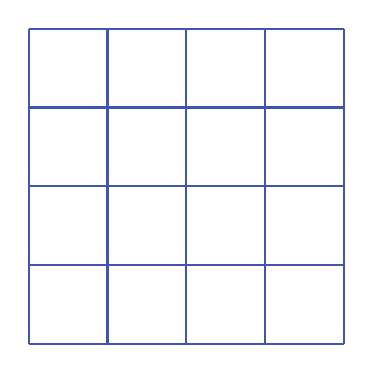
\begin{tikzpicture}
			\draw[timhieukhoahoc,thick] (0,0) grid (4,4);
		\end{tikzpicture}
	\end{center}
	\centerline{\textbf{\color{toancuabi}Khám phá vùng đất mới bằng Kinh khí cầu}}
	\vskip 0.1cm
	\textit{Biết Tuốt thích đọc sách, cậu đã đọc rất nhiều sách kể chuyện những xứ sở xa xăm cũng như về các chuyến du lịch. Mỗi khi rỗi rãi, chú lại kể cho các bạn của mình nghe. Các chú tí hon rất thích nghe nói đến những đất nước kì lạ mà chưa từng được trông thấy bao giờ. Biết Tuốt kể cho các chú nghe nhiều đến nỗi các chú đâm ra mơ mộng, mơ mộng được đi du lịch một phen. Và một ngày, Biết Tuốt nói mình sẽ sáng tạo ra một cái khinh khí cầu để bay lên bầu trời đi du lịch. Ý kiến tuyệt quá, các chú tí hon vô cùng thích thú và đã sẵn sàng cùng Biết Tuốt sáng tạo ra kinh khí cầu.}
	\vskip 0.1cm
	Nào chúng ta cùng Biết Tuốt và các bạn làm kinh khí cầu và khám phá vùng đất mới qua những bài toán sau nhé.
	\vskip 0.1cm
	\textbf{\color{toancuabi}Câu chuyện $\pmb{5.}$} Biết Tuốt quyết định làm một quả kinh khí cầu bằng cao su, cậu giao cho các chú tí hon khác đi kiếm nhựa cây về để tạo thành cao su. Mít Đặc rủ Viên Đạn đi lấy nhựa cây ở một quả đồi gần nhà. Hai chú đã leo lên đỉnh đồi với vận tốc $2$km trên giờ và quay xuống với vận tốc $6$km trên giờ. Các chú đã mất $4$ tiếng để leo lên và đi xuống quả đồi. Các bạn tính xem tổng quãng đường hai chú phải đi (lên đỉnh dốc và đi xuống chân dốc) của $2$ chú là bao nhiêu nhé.
	\vskip 0.1cm
		\begin{wrapfigure}{r}{0.4\linewidth}
		\centering
		\vspace*{-15pt}
		\captionsetup{labelformat= empty, justification=centering}
		\includegraphics[width=1\linewidth]{Hinh8_LayNhua}
		%\caption{\textit{\color{toancuabi}Hình $8$.}}
		\vspace*{-15pt}
	\end{wrapfigure}
	\textbf{\color{toancuabi}Câu chuyện $\pmb{6.}$} Sau khi làm xong quả kinh khí cầu, Biết Tuốt còn bảo các chú tí hon chuẩn bị cát mang lên kinh khí cầu, làm dù để phòng sự cố xảy ra khi đang bay. Không những thế Biết Tuốt còn hướng dẫn các bạn luyện tập những thao tác cần thiết trước khi lên đường. Buổi sáng hôm đó, các chú tí hon dạy từ sáng sớm và bắt đầu luyện tập từ $7$ giờ. Các chú mất $25$ phút học cách đứng thăng bằng trên kinh khí cầu, mất $\frac{3}{4}$ giờ để xếp các bao cát và ném bao cát xuống khi cần thiết và $1\frac{1}{2}$ để học cách nhảy dù. Các chú đã luyện tập không ngừng nghỉ suốt từ $7$ giờ $40$ phút sáng, mấy giờ các chú ấy mới luyện tập xong các bạn nhỉ?
	\begin{multicols}{2}
		\begin{figure}[H]
			\centering
			\vspace*{-5pt}
			\captionsetup{labelformat= empty, justification=centering}
			\includegraphics[width=0.98\linewidth]{Hinh9_KinhKhiCau}
			%\caption{\textit{\color{toancuabi}Hình $9$.}}
			\vspace*{-5pt}
		\end{figure}
		\textbf{\color{toancuabi}Câu chuyện $\pmb{7.}$} Ngày khởi hành cũng đã đến, các chú tí hon khăn gói quả mướp, háo hức lên đường. Quả cầu vút lên cao một cách êm ả, nó lên cao, rất cao, các chú tí hon sung sướng ngắm nhìn cảnh phía dưới. Quả cầu vượt qua bao ruộng đồng, bay qua dòng sông Dưa Chuột, vượt qua những rặng núi, xuyên qua những đám mây. Chắc Chắn được giao ghi lại lịch trình của chuyến đi, một tay chú cầm bút ghi, tay kia cầm chiếc đồng hồ, \,\,chú \,\,nói: Chúng\,\, ta\,\, khởi
	\end{multicols}
	hành lúc $8$ giờ và mất $40$ phút từ lúc đi đến lúc bay qua dòng sông Dưa Chuột, chúng ta mất thêm $60$ phút để bay qua nhiều ruộng đồng rồi đến một dãy núi, ở đây ta phải dừng lại mất $10$ phút để bỏ bớt một số bao cát giúp kinh khí cầu bay cao hơn.  Mình đã mất $80$ phút để bay qua dãy núi này. Khi vừa bay qua dãy nũi, chúng ta gặp những đám mây trắng bồng bềnh trôi, và kinh khí cầu vừa bay qua được những đám mây này mất $20$ phút. Theo kế hoạch $1$ giờ $30$ phút chiều mình sẽ tới một hòn đảo.
	\vskip 0.1cm
	\begin{wrapfigure}{r}{0.5\linewidth}
		\centering
		\vspace*{-25pt}
		\captionsetup{labelformat= empty, justification=centering}
		\includegraphics[width=1\linewidth]{Hinh23_KinhKhiCau}
		%\caption{\textit{\color{toancuabi}Hình $9$.}}
		\vspace*{-20pt}
	\end{wrapfigure}
	Cáu Kỉnh lên tiếng: Cậu kể dài dòng quá, tôi cần quan tâm còn bao lâu nữa thì chúng ra sẽ đến được hòn đảo. Chắc Chắn mới tập trung ghi chép thôi, chưa có tính ra yều cầu của Cáu Kỉnh, các bạn giúp Chắc Chắn nhé. 
	\vskip 0.1cm
	\textbf{\color{toancuabi}Câu chuyện $\pmb{8.}$} Kinh khí cầu đã đưa các chú tí hon dạo chơi trên chín tầng mây được hơn một ngày. Bao giờ thì đến thành phố mới lạ theo kế hoạch nhỉ? Biết Tuốt nói với các bạn:
	\vskip 0.1cm
	“\textit{Kinh khí cầu sẽ không đưa ta ngay lập tức đến thành phố mới mà sau một …}”, Biết Tuốt ngập ngừng. Các chú tí hon liền nhao nhao đoán: “\textit{một giây!}”, “\textit{một phút!}”, “\textit{một giờ!}”,“\textit{một ngày!}”, “\textit{một tuần!}”, “\textit{một tháng!}” Biết Tuốt nói rằng trong các câu trả lời trên thì một dự đoán là chính xác so với tính toán của cậu ấy, còn các dự đoán còn lại lần lượt sai $24$ lần, $60$ lần, $168$ lần, $720$ lần, và $3600$ lần so với tính toán. Theo tính toán của Biết Tuốt thì bao lâu nữa các bạn của chúng ta sẽ đến được thành phố mới nhỉ?
	\vskip 0.1cm
	Không biết bao lâu thì các chú tí hon mới đến thành phố mới lạ, nhưng các cô chú hon ở nhà thì ngưỡng mộ Biết Tuốt và các bạn ấy lắm. Cả thành phố ngâm nga suốt bài thơ của thi sĩ Hoa Giấy
	
	\begin{adjustwidth}{75pt}{0pt}
		\begin{flushleft}
			\textit{Quả cầu vĩ đại căng hơi\\
			Trời cao vút tới, bồi hồi lòng ta\\
			Tự hào như cánh chim xa\\
			Tầng không ta vượt, bay qua ruộng đồng\\
			Bay qua biển, bay qua sông\\
			Chúng ta đâu có nản lòng bạn ơi!}
		\end{flushleft}
	\end{adjustwidth}
	\begin{center}
		\textbf{\color{toancuabi}Những người bạn mới}
	\end{center}
	\textit{Chuyến đi trên kinh khí cầu đã không đúng như dự định vì giữa đường các bạn gặp tai nạn và cả đoàn đã phải nhảy dù ra khỏi kinh khí cầu. Các chú tí hon đã lạc đến thành phố Xanh và được các cô tí hon ở đây giúp đỡ. Thành phố Xanh có những ngôi nhà xinh đẹp, không gian ngợp trong màu lá cây xanh thắm, phố xá luôn sạch sẽ, gọn gàng. Từ tai nạn không may này mà các chú đã được làm quen với những cô tí hon hết sức dễ thương như Mắt Xanh, Bạch Tuyết, biết đến thi sĩ Hoa Dại, hay bác sĩ Mật Ngọt, …  Không những thế các chú còn được làm quen với các chú tí hon ở thành phố Diều, biết đến Đinh Ốc, nhà phát minh cừ khôi với rất nhiều phát minh kì lạ và cả nhà văn Cả Láu với những câu chuyện thú vị từ chiếc máy ghi âm.}
	\begin{figure}[H]
		\centering
		\vspace*{-5pt}
		\captionsetup{labelformat= empty, justification=centering}
		\includegraphics[width=0.5\linewidth]{Hinh11_ThanhPhoDieu}
		%\caption{\textit{\color{toancuabi}Hình $9$.}}
		\vspace*{-10pt}
	\end{figure}	
	Chúng ra cùng tham gia vào những câu chuyện của các cô chú tí hon ở hai thành phố xinh đẹp này qua những bài toán sau nhé.
	\vskip 0.1cm
	\textbf{\color{toancuabi}Câu chuyện $\pmb{9.}$} Các cô tí hon có một chiếc xe ô tô nhưng bị hỏng. Bu Loong và Đinh Vít đã quyết định sửa giúp các cô chiếc ô tô này. Do  không có đồ nghề để sửa, thế nên hai cậu sang thành phố Diều để mượn. Chú tài xế Bánh Vòng đã chở hai cậu đến nhà Đinh Ốc để mượn mỏ hàn. Nhà của Đinh Ốc nằm trên một căn phố nhỏ. Có $5$ ngôi nhà liên tiếp được đánh số lần lượt từ $1$ đến $5$ ở phố của Đinh Ốc và nhà của cậu ấy là nhà số $3$. Khi đến nơi, những chú tí hon thấy cả năm ngôi nhà có các màu sơn khác nhau: xanh, đỏ, tím, vàng, hồng. Ngôi nhà màu đỏ chỉ nằm cạnh một ngôi nhà khác. Ngôi nhà màu xanh thì nằm cạnh các ngôi nhà màu vàng và màu đỏ. Nhà của Đinh Ốc màu gì các bạn có biết không?
		\begin{figure}[H]
		\centering
		\vspace*{-5pt}
		\captionsetup{labelformat= empty, justification=centering}
		\includegraphics[width=0.6\linewidth]{Hinh24_NhaDinhOc}
		%\caption{\textit{\color{toancuabi}Hình $11$.}}
		\vspace*{-10pt}
	\end{figure}
	\textbf{\color{toancuabi}Câu chuyện $\pmb{10.}$} Ở thành phố Xanh, mỗi nhà có một hầm để chứa hoa quả. Các cô tí hon cưa các loại quả từ cây xuống và lăn về hầm, công việc khá là tốn thời gian và công sức. Nhờ có Bu Loong và Đinh Vít đã sửa chiếc ô tô mà việc vận chuyển được “cơ giới hóa”, giúp hoa quả được đưa về hầm nhanh hơn. Một ngày nọ nhóm bốn chú tí hon vận chuyển được $100$ quả táo về hầm. Mít Đặc nói: “ Tớ vận chuyển được trên $5$ quả táo đấy, nhưng tớ vẫn chuyển ít hơn Ngộ Nhỡ”. Nhanh Nhảu thì hí hửng khoe: “Thế mà tớ chuyển được hơn Ngộ Nhỡ $3$ quả đấy”. Bu Loong nói ngay: “Các cậu chuyển được nhiều táo đấy, nhưng nhờ cơ giới hóa mà số táo tớ mang về hầm gấp $3$ lần tổng số táo của cả ba cậu.” Các bạn tính xem mỗi chú tí hon vận chuyển được bao nhiêu táo nhé.
	\begin{figure}[H]
		\centering
		\vspace*{-5pt}
		\captionsetup{labelformat= empty, justification=centering}
		\includegraphics[width=0.6\linewidth]{Hinh12_ChuyenTao}
		%\caption{\textit{\color{toancuabi}Hình $12$.}}
		\vspace*{-10pt}
	\end{figure}
	\textbf{\color{toancuabi}Câu chuyện $\pmb{11.}$} Nhờ có cơ giới hóa mà công việc tiến hành dễ dàng và mau chóng. Ô tô đi lại như con thoi giữa các cây táo. Các cô tí hon không phải đẩy quả về nhà nữa nhưng không phải vì thế mà các cô ngồi chơi. Các cô đã dựng hai cái lều vải ở trong phố và đem đến nước đường và bánh mứt kẹo cho bà con lao động có thể giải khát lúc nghỉ ngơi.Lều lớn chứa được lượng người nhiều gấp đôi so với phòng nhỏ. Vào một buổi trưa,ba phần tư chỗ ngồi của hai cái lều đã kín chỗ. Sau đó, một nhóm gồm $18$ cô chú tí hon lại ghé đến lều. Thế nhưng, một cô tí hon ra thông báo rằng lều chỉ còn đủ chỗ cho một nửa số người của nhóm. Các bạn có tính được mỗi lều chứa được bao nhiêu người không?
		\begin{figure}[H]
		\centering
		\vspace*{-5pt}
		\captionsetup{labelformat= empty, justification=centering}
		\includegraphics[width=0.55\linewidth]{Hinh13_Leu}
		%\caption{\textit{\color{toancuabi}Hình $13$.}}
		\vspace*{-10pt}
	\end{figure}
	\textbf{\color{toancuabi}Câu chuyện $\pmb{12.}$} Bánh Vòng khi đưa Bu Loong và Đinh Vít trở về thành phố Xanh đã ở lại hỗ trợ các cô tí hon chuyển hoa quả, rồi Đinh Ốc cũng đến và sáng tạo ra ô tô tám bánh chạy bằng hơi nước để hỗ trợ thêm. Thành phố Xanh càng nhộn nhịp hơn khi có thêm Đinh Dép đến giúp. Đinh Dép làm việc rất hăng say và phấn khởi, ai yêu cầu gì cậu cũng vui vẻ làm. Một buổi sáng, Đinh Dép cùng Lặng Lẽ sơn lại hàng rào ở quảng trường Cây Táo. Hàng rào ở quảng trường dài $15$ mét. Đinh Dép dùng thùng sơn màu xanh, bắt đầu sơn hàng rào từ vị trí cách mép trái $2$m và sơn hàng rào từ trái sang phải. Lặng Lẽ thì dùng thùng sơn màu trắng, sơn hàng rào từ phải sang trái và hết sơn khi cách mép trái của hàng rào là $4$ mét. Biết rằng thùng sơn màu xanh sơn được tất cả $9$ mét hàng rào, còn thùng sơn màu trắng thì sơn được tất cả là $10$ mét hàng rào. Các bạn tính nhanh xem có bao nhiêu mét của hàng rào được sơn bởi đúng một lớp sơn nhé.
	\begin{figure}[H]
		\centering
		\vspace*{-5pt}
		\captionsetup{labelformat= empty, justification=centering}
		\includegraphics[width=0.55\linewidth]{Hinh14_SonRao}
		%\caption{\textit{\color{toancuabi}Hình $14$.}}
		\vspace*{-10pt}
	\end{figure}
	Quảng trường Cây Táo sắp đón một sự kiện chưa từng có đấy, các bạn đón chờ nhé.
	\vskip 0.1cm
	\centerline{\textbf{\color{toancuabi}Bữa tiệc tại thành phố Xanh}}
	\vskip 0.1cm
	Sau khi bị rơi khỏi Khinh khí cầu, các chú tí hon lạc được đến thành phố Xanh và được các cô tí hon giúp đỡ. Tất nhiên là các chú tí hon cũng giúp các cô rất nhiều việc. Hơn thế nữa, nhờ các chú mà đã hóa giải được hiểu lầm giữa các cô tí hon ở thành phố Xanh và các chú tí hon ở thành phố Diều.  Để kỷ niệm sự kiện này, các cô chú sẽ tổ chức một bữa tiệc long trọng tại quảng trường Cây Táo.
	Các em hãy cùng Mít Đặc tham gia vào bữa tiệc này nhé.
	\vskip 0.1cm
		\begin{wrapfigure}{r}{0.5\linewidth}
		\centering
		\vspace*{5pt}
		\captionsetup{labelformat= empty, justification=centering}
		\includegraphics[width=1\linewidth]{Hinh15_BachTuyet}
		%\caption{\textit{\color{toancuabi}Hình $15$.}}
		\vspace*{-15pt}
	\end{wrapfigure}
	\textbf{\color{toancuabi}Câu chuyện $\pmb{13.}$} Tất cả mọi người bắt tay vào việc chuẩn bị cho bữa tiệc. Người thì xén bớt cỏ để làm sân nhảy, người thì dựng lầu để biểu diễn nhạc, xa một chút là một dãy lều dùng để chứa nước ngọt và bánh kẹo. Bạch Tuyết phụ trách việc mua bánh cho bữa tiệc. Cô được giao $100$ đồng để mua và dự định mua hai loại bánh xu kem và bánh gato. Cửa hàng bánh bán $1$ đồng được hai bánh xu kem còn bánh gato giá $13$ đồng một chiếc. Bạch Tuyết có thể mua $100$ chiếc bánh với số tiền đó không các bạn nhỉ?
	\vskip 0.1cm
	\begin{wrapfigure}{l}{0.5\linewidth}
		\centering
		\vspace*{-5pt}
		\captionsetup{labelformat= empty, justification=centering}
		\includegraphics[width=1\linewidth]{Hinh16_ThuocNuoc}
		%\caption{\textit{\color{toancuabi}Hình $16$.}}
		\vspace*{-10pt}
	\end{wrapfigure}
	\textbf{\color{toancuabi}Câu chuyện $\pmb{14.}$} Mặc dù phần lớn các chú tí hon đã ra khỏi bệnh viện, Thuốc Viên vẫn chưa được ra do không nghe lời bác sĩ Mật Ngọt. Cậu tìm cách trốn đến nhà Mít Đặc sớm để đi dự tiệc cùng các bạn. Trên đường, cậu nhẩm tính và tự bảo: nếu giữ nguyên vận tốc thế này thì mình sẽ đến chỗ Mít Đặc $8$ phút trước khi Mít Đặc rời nhà đi dự tiệc. Thật không may, giữa đường cậu nhận ra là mình chưa thay bộ quần áo bệnh viện nên phải quay lại. Vì việc này mà cậu đến chỗ Mít Đặc muộn hơn $10$ phút so với dự định. Hỏi Thuốc Viên đã đi được bao nhiêu phần của quãng đường khi phát hiện ra mình quên thay quần áo, biết rằng tổng thời gian đi của cậu là $38$ phút?
		
	\textbf{\color{toancuabi}Câu chuyện $\pmb{15.}$} Trong bữa tiệc, các chú Tí hon rủ các cô tí hon chơi trò domino, mỗi người tham gia trò chơi sẽ được phát $2$ quân domino. Bạch Tuyết thông báo là có $40$ cô tí hon muốn chơi trò chơi này. Tuy nhiên, bộ domino các chú tí hon mang theo chỉ có $28$ quân, mỗi quân có hai ô, mỗi ô có từ $0$ đến $6$ chấm, và không có hai quân domino nào giống hệt nhau. Mít Đặc đề xuất là sẽ làm bộ domino mới với số chấm thay đổi từ $0$ đến $12$. Các bạn tính thử xem với đề xuất của Mít Đặc thì bộ domino mới có đủ để phát cho $40$ cô tí hon tham gia chơi không nhé.
	\begin{figure}[H]
		\centering
		\vspace*{-5pt}
		\captionsetup{labelformat= empty, justification=centering}
		\includegraphics[width=0.6\linewidth]{Hinh17_Domino}
		%\caption{\textit{\color{toancuabi}Hình $17$.}}
		\vspace*{-10pt}
	\end{figure}
	\textbf{\color{toancuabi}Câu chuyện $\pmb{16.}$} Cuối buổi tiệc, khách khứa đều được tặng những hộp kẹo đem về. Nhanh Nhảu đề nghị một trò chơi: Đầu tiên cậu ấy sẽ cho Mít Đặc gấp đôi số kẹo mà Mít Đặc có, sau đó lại lấy lại $8$ chiếc. Mít Đặc nghĩ một lúc, thấy có vẻ hời nên đồng ý. Sau $3$ lần trao đổi như thế Mít Đặc thấy trong hộp của mình không còn chiếc kẹo nào. Thật là tai hại! Các bạn tính xem lúc đầu Mít Đặc có bao nhiêu chiếc kẹo nhé.
	\begin{figure}[H]
		\centering
		\vspace*{-5pt}
		\captionsetup{labelformat= empty, justification=centering}
		\includegraphics[width=0.4\linewidth]{Hinh18_MitDac}
		%\caption{\textit{\color{toancuabi}Hình $18$.}}
		\vspace*{-10pt}
	\end{figure}
	\centerline{\textbf{\color{toancuabi}Tạm biệt thành phố Xanh}}
	\vskip 0.1cm
	\begin{multicols}{2}
		\textit{Sau một thời gian lưu trú tại thành phố Xanh, các chú tí hon đã quyết định trở về thành phố Hoa của mình. Các cô chú tí hon đã rất buồn khi phải tạm biệt nhau. Để lưu thành những kỷ niệm, nhiều hoạt động đã diễn ra: Kèn Đồng sáng tác nhạc và Hoa Dại làm thơ tặng các bạn mình, các cô tí hon đã may túi tặng các chú tí hon rồi các cô chú cùng nhau tổ chức một buổi vũ hội,\ldots Các bạn nhỏ hãy cùng các cô chú tí hon tham gia vào các hoạt động này qua các bài toán dưới đây nhé.}
		\begin{figure}[H]
			\centering
			\vspace*{-5pt}
			\captionsetup{labelformat= empty, justification=centering}
			\includegraphics[width=1\linewidth]{Hinh10_ThanhPhoXanh}
			%\caption{\textit{\color{toancuabi}Hình $18$.}}
			\vspace*{-10pt}
		\end{figure}
	\end{multicols}
	\vskip 0.1cm
		\begin{wrapfigure}{l}{0.5\linewidth}
		\centering
		\vspace*{-5pt}
		\captionsetup{labelformat= empty, justification=centering}
		\includegraphics[width=1\linewidth]{Hinh19_KenDong_HoaGiay}
		\vspace*{-15pt}
	\end{wrapfigure}
	\textbf{\color{toancuabi}Câu chuyện $\pmb{17.}$} Sắp đến thời gian các chú tí hon phải trở về thành phố Hoa, nhạc sĩ Kèn Đồng sáng tác một bài hát và thi sĩ Hoa Dại làm một bài thơ tặng các bạn của mình. Vì nóng lòng muốn khoe ngay tác phẩm mình vừa sáng tác, sáng sớm hôm sau, hai bạn cùng đi sớm nhất có thể (thế nên cùng thời điểm) để đến nhà nhau. Vì mải hát và ngâm thơ dọc đường nên hai bạn không nhìn thấy nhau tại lúc gặp nhau giữa đường. Sau thời điểm gặp, Hoa Dại đến nhà Kèn Đồng sau đó $4$ phút, còn Kèn Đồng đến nhà Hoa Dại sau đó $1$ phút. Các bạn hãy tính xem mỗi thi sĩ đã đi đến nhà nhau mất bao nhiêu phút nhé.
	\newpage
	\begin{wrapfigure}{l}{0.5\linewidth}
		\centering
		\vspace*{5pt}
		\captionsetup{labelformat= empty, justification=centering}
		\includegraphics[width=1\linewidth]{Hinh20_TangTui}
		%\caption{\textit{\color{toancuabi}Hình $20$.}}
		\vspace*{-10pt}
	\end{wrapfigure}
	\textbf{\color{toancuabi}Câu chuyện $\pmb{18.}$} Để làm kỷ niệm, Mắt Xanh và một số cô tí hon trong thành phố Xanh đã may túi tặng các chú tí hon. Mỗi cô trong nhóm đã may được một số lượng túi như nhau và cùng nhau mang túi đến tập hợp ở nhà Bạch Tuyết. Trên đường đi, các cô gặp một nhóm các chú tí hon và thật trùng họp số chú tí hon trong nhóm đúng bằng số các cô tí hon, mỗi cô đã tặng mỗi chú tí hon một chiếc túi mà mình may được. Sau khi tặng túi, mỗi cô tí hon vẫn còn hơn $1$ chiếc và tập hợp tất cả lại được $33$ chiếc mang đến nhà Bạch Tuyết. Các bạn có tính được mỗi cô tí hon đã may bao nhiêu chiếc túi không?
	\vskip 0.1cm
	\begin{wrapfigure}{r}{0.5\linewidth}
		\centering
		\vspace*{-5pt}
		\captionsetup{labelformat= empty, justification=centering}
		\includegraphics[width=1\linewidth]{Hinh21_VongTron}
		\vspace*{-15pt}
	\end{wrapfigure}	
	\textbf{\color{toancuabi}Câu chuyện $\pmb{19.}$} Một buổi vũ hội đã được tổ chức trước ngày các chú tí hon trở về. Cuối buổi, các cô chú tí hon xếp thành một vòng tròn để nghe hai Kèn Đồng biểu diễn nhạc và Hoa Dại đọc thơ. Mít Đặt và Tròn Xoay mải chạy loanh quanh nên không kịp tham gia vào vòng tròn này. Tròn Xoay nói: “Tớ chưa từng thấy nhiều người trong một vòng tròn như thế. Chúng ta đếm thử xem có bao nhiêu người nhé.” Mít Đặc và Tròn Xoay cùng đi theo một chiều để đếm số người trong vòng tròn nhưng bắt đầu từ những người khác nhau. Người thứ $20$ theo cách đếm của Mít Đặc lại là người thứ $7$ theo cách đếm của Tròn Xoay, còn người thứ $7$ theo cách của đếm của Mít Đặc lại là người thứ $94$ theo cách của Tròn Xoay. Thế thì vòng tròn này có bao nhiêu cô chú tí hon nhỉ? Các bạn có tính được không?
	\vskip 0.1cm
	\textbf{\color{toancuabi}Câu chuyện $\pmb{20.}$} Khi chia tay với các cô tí hon, Mít Đặc hứa là sẽ viết thư cho Mắt Xanh, thế nên từ khi trở về thành phố Hoa, cậu chịu khó luyện viết lắm, dạo này cậu còn học thêm cả toán nữa. Trong bức thư trước, Mắt Xanh hỏi bao giờ thì các chú làm xong kinh khí cầu để quay lại thăm thành phố Xanh. Trong bức thư lần này gửi cho Mắt Xanh, Mít Đặc được dịp thể hiện luôn, cậu viết: “Chúng tớ đang làm kinh khí cầu rồi. Biết Tuốt đã dự tính một số ngày. Nếu mỗi người bọn tớ làm $6$ ngày công thì sẽ thừa ra $20$ ngày, còn nếu mỗi người chỉ làm $4$ ngày công thì vừa đủ so với dự tính. Cậu thử tính xem Biết Tuốt dự kiến bao nhiêu ngày.” Các bạn hãy tính cùng Mắt Xanh nhé.
	\begin{figure}[H]
		\centering
		\vspace*{-5pt}
		\captionsetup{labelformat= empty, justification=centering}
		\includegraphics[width=0.35\linewidth]{Hinh22_MitDacLamToan}
		\vspace*{-10pt}
	\end{figure}
	Mít Đặc và những cô chú tí hon đáng yêu đã tham gia vào những cuộc phiêu lưu thật là thú vị phải không các em? Các em hãy đồng hành cùng các cô chú tí hon trong những cuộc phiêu lưu ấy bằng cách giải những bài toán ở trên nhé. 
	\begin{center}
		\textit{Quả cầu vĩ đại căng hơi\\
			Trời cao vút tới, bồi hồi lòng ta\\
			Tự hào như cánh chim xa\\
			Tầng không ta vượt, bay qua ruộng đồng\\
			Bay qua biển, bay qua sông\\
			Chúng ta đâu có nản lòng bạn ơi!}
	\end{center}
	\newpage

	\thispagestyle{empty}
	\begingroup 
	\AddToShipoutPicture*{\put(0,0){\includegraphics[width=17.2cm]{../dovui/Do_vui_Pi7_2019}}}
	\centering
	\vspace*{0cm}
	\endgroup
	\newpage	
	
	\thispagestyle{empty}
	\begin{center}
		\textbf{\Large\color{toancuabi}PHẦN III. SUY LUẬN CÙNG BI}
	\end{center}
	\newpage

	
\graphicspath{{../suyluancungbi/sumi/}}
\begingroup
\AddToShipoutPicture*{\put(130,420){\includegraphics[scale=0.75]{sumitd.pdf}}} % %Image background
\AddToShipoutPicture*{\put(20,60){\includegraphics[scale=0.75]{shape1.pdf}}} % %Image background
\AddToShipoutPicture*{\put(70,235){\includegraphics[scale=0.75]{cd1.pdf}}} % %Image background
\AddToShipoutPicture*{\put(48,100){\includegraphics[scale=0.3]{h1}}} % %Image background
\centering
\endgroup
\vspace*{120pt}

	\textbf{\textit{Sumi và Jenny là một đôi bạn rất  thân và đặc biệt là cả hai bạn đều rất thích học  Toán. Chú Jason, bố của Jenny là một thầy giáo dạy Toán nên có rất nhiều các câu đố vui hóc búa để thử thách các  bạn nhỏ. 
	\vskip 0.2cm
	Hôm nay Sumi sang chơi nhà Jenny. Như thường lệ, điều Sumi chờ đợi nhất chính là những câu đố của chú Jason.
	\vskip 0.2cm
	Không để các bạn phải đợi lâu, chú Jason lấy ra một chiếc mũ màu đỏ, một chiếc mũ màu xanh, và bắt đầu chuỗi câu đố của mình.}}	

\begin{adjustwidth}{120pt}{0pt}
	-- Hai con hãy nhắm mắt lại một lúc, để ta có thể đội cho mỗi người một chiếc mũ nhé! -- Chú Jason nói
	-- Được rồi, các con có thể mở mắt ra. Sumi, con có biết mũ của mình màu gì không?
	\vskip 0.1cm
	Sumi nhìn Jenny và trả lời ngay lập tức:
	\vskip 0.1cm
	-- Màu đỏ ạ.
	\vskip 0.1cm
	-- Tại sao con lại biết mũ của mình màu đỏ? -- Chú Jason hỏi tiếp.
	\vskip 0.1cm
	-- Con thấy Jenny đội mũ màu xanh, nên chiếc mũ của con phải là màu đỏ ạ. -- Sumi trả lời.
\end{adjustwidth}
%\newpage
%\begingroup
%\AddToShipoutPicture*{\put(0,295){\includegraphics[scale=1]{shape2.pdf}}} % %Image background
%\AddToShipoutPicture*{\put(80,545){\includegraphics[scale=0.75]{cd2.pdf}}} % %Image background
%\AddToShipoutPicture*{\put(240,-10){\includegraphics[scale=0.75]{shape3.pdf}}} % %Image background
%\AddToShipoutPicture*{\put(350,725){\includegraphics[scale=0.75]{cd3.pdf}}} % %Image background
%\AddToShipoutPicture*{\put(70,330){\includegraphics[scale=0.25]{sumi/h2}}} % %Image background
%\AddToShipoutPicture*{\put(340,365){\includegraphics[scale=0.25]{sumi/h3}}} % %Image background
%\AddToShipoutPicture*{\put(70,25){\includegraphics[scale=0.25]{sumi/h5}}} % %Image background
%\AddToShipoutPicture*{\put(340,20){\includegraphics[scale=0.25]{sumi/h4}}} % %Image background
%\AddToShipoutPicture*{\put(110,275){\includegraphics[scale=0.75]{cd5.pdf}}}
%\AddToShipoutPicture*{\put(350,325){\includegraphics[scale=0.75]{cd4.pdf}}} % %Image background
%\centering
%\endgroup
%\begin{adjustwidth}{0pt}{80pt}
	\textbf{Câu đố 2}
	\vskip 0.1cm
	Chú Jason lấy thêm một chiếc mũ màu đỏ. Chú lại yêu cầu hai bạn nhắm mắt lại, và đội cho mỗi bạn một chiếc mũ. Sau đó, chú giấu chiếc mũ còn lại đi.
	\vskip 0.1cm
	-- Bây giờ, các con mở mắt ra nào. Sumi, con có biết mũ của mình màu gì không? -- Chú  Jason hỏi.
	\vskip 0.1cm
	-- Dạ không ạ. -- Sumi nhìn Jenny, nhưng lần này cậu không đoán được màu mũ của mình.
	\vskip 0.1cm
	-- Còn Jenny, con có biết mình đội mũ màu  gì không?”
	\vskip 0.1cm
	-- Màu đỏ ạ. -- Jenny trả lời ngay lập tức.
	\vskip 0.1cm
	-- Con hãy giải thích cho bố xem tại sao nào?
	\vskip 0.1cm
	-- Nếu con đội mũ màu xanh thì chỉ còn lại hai chiếc mũ màu đỏ, và khi đó Sumi sẽ biết ngay là bạn ý đội chiếc mũ màu đỏ ạ. Do Sumi không đoán được bạn ý đội mũ màu gì, nên chiếc mũ của con phải là màu đỏ ạ. – Jenny giải thích.
%	\end{adjustwidth}
		\begin{figure}[H]
		\centering
		\vspace*{-5pt}
		\captionsetup{labelformat= empty, justification=centering}
		\includegraphics[width=0.5\textwidth]{h2}
		\vspace*{-10pt}
		\end{figure}
	\textbf{Câu đố 3}
	\vskip 0.1cm
	Đúng lúc này thì bé Julia đi học về, và đòi chơi cùng anh Sumi và chị Jenny. Chú Jason yêu cầu ba bạn nhỏ nhắm mắt lại và dùng hai chiếc mũ đỏ, một chiếc mũ xanh để đội cho mỗi bạn một chiếc mũ.
	\vskip 0.1cm
	-- Các con mở mắt ra nào. Sumi, con có biết mũ của mình màu gì không?
	\vskip 0.1cm
	-- Màu xanh ạ! -- Sumi trả lời rất nhanh.
	\vskip 0.1cm
	-- Con cũng đội mũ màu xanh ạ! -- Julia  nhanh nhẩu.
	\vskip 0.1cm
	-- Màu xanh? Con có chắc không, Julia? -- Chú Jason hỏi lại.
	\vskip 0.1cm
	-- Ah, con bị nhầm rồi ạ. Bố dùng hai chiếc mũ đỏ, một chiếc mũ xanh. Anh Sumi đội mũ xanh, chị Jenny đội mũ đỏ, như vậy con sẽ đội mũ đỏ ạ. – Julia sửa lại.
	\begin{figure}[H]
	\centering
	\vspace*{-5pt}
	\captionsetup{labelformat= empty, justification=centering}
	\includegraphics[width=0.5\textwidth]{h3}
	\vspace*{-10pt}
	\end{figure}
	
	\textbf{Câu đố 4}
	\vskip 0.1cm
	-- Tốt lắm! Bây giờ sẽ là một thử thách khó hơn cho các con. -- Chú Jason nói; rồi chú lấy thêm một chiếc mũ đỏ và một chiếc mũ xanh. Như vậy, có tổng cộng ba chiếc mũ đỏ và hai chiếc mũ xanh trên bàn. Chú lại yêu cầu cả ba bạn nhắm mắt lại, rồi đội cho mỗi bạn một chiếc mũ. Sau đó, chú giấu hai chiếc mũ còn lại đi.
	\vskip 0.1cm
	-- Jenny, con có biết mình đội mũ màu gì không?
	\vskip 0.1cm
	-- Con đội mũ đỏ ạ. -- Jenny trả lời.
	\vskip 0.1cm
	-- Vậy thì con đội mũ màu xanh rồi. -- Sumi  nói tiếp.
	\vskip 0.1cm
	Theo các bạn, Sumi nói có đúng không? Vì sao?
	\begin{figure}[H]
		\centering
		\vspace*{-5pt}
		\captionsetup{labelformat= empty, justification=centering}
		\includegraphics[width=0.5\textwidth]{h5}
		\vspace*{-10pt}
	\end{figure}
	
	\textbf{Câu đố 5}
	\vskip 0.1cm
	Các bạn nhỏ đòi chú Jason đố thêm một lần nữa. Chú vẫn dùng ba chiếc mũ đỏ và hai chiếc mũ xanh để đội cho mỗi bạn một chiếc.
	\vskip 0.1cm
	-- Sumi, con có biết mình đội mũ màu gì không?
	\vskip 0.1cm
	-- Còn Jenny, con đội mũ màu gì?
	\vskip 0.1cm
	-- Con cũng không biết ạ. -- Jenny lắc đầu.
	\vskip 0.1cm
	-- Vậy thì Julia, con đội mũ màu gì?
	\vskip 0.1cm
	Các bạn hãy giúp Julia trả lời câu hỏi nhé!
	\begin{figure}[H]
		\centering
		\vspace*{-5pt}
		\captionsetup{labelformat= empty, justification=centering}
		\includegraphics[width=0.5\textwidth]{h4}
		\vspace*{-10pt}
	\end{figure}
	\newpage
\graphicspath{{../suyluancungbi/sudoku1/}}
\begingroup
\AddToShipoutPicture*{\put(62,600){\includegraphics[scale=1]{../sudoku1/sudokutieude1.pdf}}} % %Image background
\centering
\endgroup
\vspace*{20pt}

	\begin{multicols}{2}
		\textbf{\color{toancuabi}Sudoku}, ban đầu có tên gọi là \textbf{\color{toancuabi}Number Place}, là một trò chơi với câu đố điền các số vào các ô trống của một bảng ô vuông có $9$ hàng và $9$ cột (gọi vắn tắt là bảng $9\times 9$), sao cho trong mỗi hàng, mỗi cột đều có tất cả các số tự nhiên từ $1$ đến $9$, và đồng thời, khi chia bảng to $9\times9$ thành chín bảng con $3\times 3$ (tức, bảng có $3$ hàng và $3$ cột) thì trong mỗi bảng con $3\times 3$ cũng có tất cả các số tự nhiên từ $1$ đến $9$. Trong Hình $1$ là một bảng $9\times 9$ và chín bảng con $3\times 3$ được phân chia ra từ bảng $9\times 9$ đó.
		\begin{figure}[H]
			\vspace*{-5pt}
			\centering
			\captionsetup{labelformat=empty, justification=centering}
			\includegraphics[scale=0.35]{hinh1}
			\caption{\textit{\small Hình $1.$}}
			\vspace*{-5pt}
		\end{figure}
	\end{multicols}
	Sudoku đã xuất hiện ở Pháp vào cuối thế kỷ $19$, nhưng sau đó lại biến mất. Đến năm $1979$, nó xuất hiện trên tạp chí Dell ở Mỹ dưới cái tên Number Place. Sau đó, nó được Nikoli đem về Nhật Bản vào năm $1984$ và đặt cho cái tên  \includegraphics[scale=0.4]{sudoku} (đọc là: Suuji wa dokushin ni kagiru), mà có thể dịch là “các số chỉ được xuất hiện một lần”. Sau này, cái tên này được Maki Kaji viết gọn lại là Sudoku. Từ đó, Sudoku sớm trở thành một trò chơi được ưa chuộng nhất ở Nhật Bản. Mãi cho đến đầu thế kỷ $21$, thế giới mới bắt đầu biết đến Sudoku một cách rộng rãi, khởi đầu từ Anh, sau đó lan sang châu Âu, châu Mỹ.
	\vskip 0.1cm
	Trong bài viết này, trước tiên Bi giới thiệu với các bạn đọc nhỏ tuổi một phiên bản của trò chơi trí tuệ Sudoku; đó là, \textbf{\color{toancuabi}phiên bản hình ảnh}. Phiên bản này rất thích hợp cho các bé từ $5$ đến $7$ tuổi.
	\vskip 0.1cm
	Đối với các bé $5$ hoặc $6$ tuổi, trò chơi sẽ trở nên hấp dẫn hơn, nếu các vị phụ huynh sử dụng thêm các tấm card hình học, hoa quả hoặc bất kì đồ vật gì có sẵn (bút chì, thước kẻ, tẩy, \ldots).
	\vskip 0.15cm
	Giờ, chúng mình cùng Bi trải nghiệm  Sudoku nhé!
	\begin{multicols}{2}
		\textbf{\color{toancuabi}Ví dụ $\pmb 1.$} Vẽ thêm hình vuông, hình tròn hoặc hình tam giác vào các ô vuông còn trống trong bảng ở Hình $2$, sao cho mỗi hình chỉ xuất hiện đúng một lần trong mỗi hàng, cũng như trong mỗi cột.
		\begin{figure}[H]
			\vspace*{5pt}
			\centering
			\captionsetup{labelformat=empty, justification=centering}
			\includegraphics[scale=0.33]{hinh2}
			\caption{\textit{\small Hình $2.$}}
			\vspace*{-10pt}
		\end{figure}
	\end{multicols}
	\textbf{\color{toancuabi}Cùng Bi suy luận:}
	\vskip 0.15cm
	-- Rõ ràng, với mỗi ô còn trống, chúng mình sẽ phải cân nhắc các khả năng điền, rồi lựa chọn hình thích hợp để điền. Vì thế, chúng mình nên bắt đầu từ những ô mà số khả năng điền phải cân nhắc là ít hơn cả, các bé nhỉ? Chúng mình biết rằng, vì trong mỗi hàng, cũng như mỗi cột, phải có đủ cả ba loại hình, nên hình điền ở ô này sẽ “áp đặt” hình nằm ở ô kia. Vì thế, ô trống nằm ở hàng hay cột nào đã có nhiều hình được điền sẽ có số khả năng điền cần cân nhắc ít hơn cả, phải không các bé?
	\vskip 0.15cm
	-- Nhìn bảng ở Hình $2$, chúng mình thấy, có hai hàng và một cột, mà mỗi hàng hay cột đều có sẵn hai hình, nói cách khác, đều chỉ có một ô trống. Với những suy luận ở trên, chắc chắn chúng mình phải bắt đầu từ những ô trống ở hai hàng và cột đó rồi!
	\vskip 0.15cm
	-- Cùng xem nào! Ở hàng trên cùng, đã có hình tròn và hình vuông ở hai ô, vậy thì ở ô trống còn lại chắc chắn phải là hình tam giác rồi! Ở hàng dưới cùng, đã có hình tam giác và hình vuông, nên ở ô trống còn lại chắc chắn phải là hình tròn. Cũng như vậy, ở cột đầu tiên (tính từ trái qua phải), đã có hình tam giác và hình tròn, do đó, ở ô trống còn lại bắt buộc phải là hình vuông.
	\vskip 0.15cm
	-- A ha! Chúng mình đã khám phá ra rồi, nếu trong một hàng hay cột đã có hai ô có hình thì ắt sẽ biết hình phải có trong ô trống còn lại là hình gì.
	\vskip 0.15cm
	-- Với khám phá trên, bằng cách xét các cột thứ hai và thứ ba, chúng mình sẽ dễ dàng điền được hình vào các ô trống còn lại sau bước điền nói trên, phải không nào?
	\vskip 0.15cm
	Các bé xem cách điền hình nêu trên của chúng mình, được thể hiện ở Hình $3$ nhé.
		\begin{figure}[H]
			\centering
			\vspace*{-10pt}
			\captionsetup{labelformat= empty, justification=centering}
			\includegraphics[width=0.48\textwidth]{hinh3}
			\caption{\small\textit{Hình $3.$}}
			\vspace*{-5pt}
		\end{figure}
	Việc giải các sudoku cũng hấp dẫn đấy chứ nhỉ! Giờ hãy cùng Bi thử sức với một sudoku  khác nha!
	\vskip 0.1cm
	\begin{wrapfigure}{l}{0.45\linewidth}
		\vspace*{-10pt}
		\centering
		\captionsetup{labelformat=empty, justification=centering}
		\includegraphics[scale=0.4]{hinh4}
		\caption{\textit{\small Hình $4.$}}
		\vspace*{-15pt}
	\end{wrapfigure}
	\textbf{\color{toancuabi}Ví dụ $\pmb2.$} Vẽ thêm quả cam, quả táo hoặc quả chuối vào các ô vuông còn trống trong bảng ở Hình $4$, sao cho mỗi loại quả chỉ xuất hiện đúng một lần trong mỗi hàng, cũng như trong mỗi cột.
	\vskip 0.1cm
	\textbf{\color{toancuabi}Cùng Bi suy luận:}
	\vskip 0.15cm
	\begin{wrapfigure}{r}{0.45\linewidth}
		\centering
		\vspace*{-5pt}
		\captionsetup{labelformat= empty, justification=centering}
		\includegraphics[width=0.45\textwidth]{hinh5}
		%\vspace*{-5pt}
		\caption{\small\textit{Hình $5.$}}
		\vspace*{-5pt}
	\end{wrapfigure}
	-- Quan sát bảng ở Hình $4$, chúng mình không thấy một hàng hay một cột nào, mà ở đó đã có sẵn hai loại quả. Ở hàng nào, cột nào cũng chỉ có đúng một loại quả mà thôi. Thế nghĩa là,  tình huống ở ví dụ này không tương tự như tình huống ở ví dụ $1$ rồi! Phải làm sao bây giờ?
	\vskip 0.1cm	
	-- Suy đi, tính lại, Bi thấy không còn cách nào khác, ngoài cách chọn một ô trống nào đó, rồi cân nhắc các khả năng điền có thể (xem Hình $5$). Các bé có đồng ý với Bi không?
	\vskip 0.1cm
	Hình $6$ thể hiện sự suy xét của Bi khi cân nhắc các khả năng điền đấy. Các bé xem nhé.
	\begin{figure}[H]
		\centering
		\vspace*{-5pt}
		\captionsetup{labelformat= empty, justification=centering}
		\includegraphics[width=0.3\textwidth]{hinh6a}\hfill
		\includegraphics[width=0.3\textwidth]{hinh6b}\hfill
		\includegraphics[width=0.3\textwidth]{hinh6c}
		\caption{\small\textit{Hình $6.$}}
		\vspace*{-10pt}
	\end{figure}
	\begin{multicols}{2}
	-- Vui quá, vậy là chúng mình đã cùng Bi điền được quả vào một ô trống rồi (xem Hình $7$).
		\begin{figure}[H]
		\vspace*{-5pt}
		\centering
		\captionsetup{labelformat=empty, justification=centering}
		\includegraphics[scale=0.4]{hinh7}
		\caption{\textit{\small Hình $7.$}}
		\vspace*{-5pt}
		\end{figure}
		-- Sudoku trái cây giờ đã trở nên đơn giản hơn, tương tự như ở ví dụ $1$ rồi. Nghĩa là, trong bảng đã có những hàng, những cột mà ở mỗi hàng hay cột đó đều chỉ có một ô trống. Vì thế, bằng các suy luận tương tự như khi giải ví dụ $1$, chúng mình đã có thể tiếp tục điền các loại quả thích hợp vào các ô trống còn lại. Các bé tự làm tiếp nhé.
	\end{multicols}
	\vskip 0.1cm
	Nhìn lại các suy luận ở trên, khi giải ví dụ $2$, Bi nhận thấy rằng, chúng mình điền được quả vào ô trống đầu tiên là do ô đó nằm ở giao của đúng một hàng và đúng một cột, mà ở hàng, cũng như ở cột ấy, lại đã có sẵn một loại quả. A ha, để ý rằng ô nào trong bảng cũng nằm ở giao của đúng một hàng và đúng một cột, chúng mình đã cùng Bi có thêm một khám phá nữa rồi. Đó là, chúng mình sẽ xác định được loại quả nằm ở một ô bất kỳ, nếu biết loại quả nằm trong hàng và trong cột chứa ô đó!
	\vskip 0.1cm
	Hiểu các suy luận của Bi khi giải các ví dụ $1$ và $2$ rồi, bây giờ các bé hãy tập tự mình suy luận để vượt qua các Sudoku dưới đây nhé.
	\vskip 0.1cm
	\textbf{\color{toancuabi}Bài tập $\pmb{1.}$} Vẽ thêm quả đào, quả nho hoặc quả xoài vào các ô vuông còn trống trong bảng ở Hình $8$, sao cho mỗi loại quả chỉ xuất hiện đúng một lần trong mỗi hàng, cũng như trong mỗi cột.
	\vskip 0.3cm
	\begin{figure}[H]
		\vspace*{-5pt}
		\centering
		\captionsetup{labelformat=empty, justification=centering}
		\includegraphics[width=0.30\textwidth]{hinh8}\hspace{40pt}
		%\includegraphics[width=0.25\textwidth]{hinh9}\hfill
		\includegraphics[width=0.30\textwidth]{hinh10}

		\caption{\textit{\small Hình $8.$ \hspace*{100pt} Hình $9.$}} % \hspace*{75pt} Hình 10
		\vspace*{-10pt}
	\end{figure}
	\textbf{\color{toancuabi}Bài tập $\pmb{2.}$} Vẽ thêm que kem, miếng bánh, cái kẹo sữa hoặc cái kẹo ngọt vào các ô vuông còn trống trong bảng ở Hình $9$, sao cho mỗi loại kem, bánh, kẹo chỉ xuất hiện đúng một lần trong mỗi hàng, cũng như trong mỗi cột.
	\vskip 0.1cm
	\textbf{\color{toancuabi}Bài tập $\pmb{3.}$} Vẽ thêm quả cà chua, quả dưa chuột, củ cà rốt hoặc quả cà tím vào các ô vuông còn trống trong bảng ở Hình $10$, sao cho mỗi loại củ, quả chỉ xuất hiện đúng một lần trong mỗi hàng, cũng như trong mỗi cột.
		\begin{figure}[H]
		\vspace*{-5pt}
		\centering
		\captionsetup{labelformat=empty, justification=centering}
		\includegraphics[width=0.3\textwidth]{hinh11}\hspace{40pt}
	%	\includegraphics[width=0.3\textwidth]{hinh12}\hfill
		\includegraphics[width=0.3\textwidth]{hinh13}
		
		\caption{\textit{\small Hình $10.$ \hspace*{75pt} Hình $11.$ }}  %\hspace*{75pt} Hình 13
		\vspace*{-10pt}
	\end{figure}
	\textbf{\color{toancuabi}Bài tập $\pmb{4.}$} Vẽ thêm  hình tam giác, hình vuông,  hình ngũ giác, hình ngôi sao hoặc hình tròn vào các ô vuông còn trống trong bảng ở Hình $11$, sao cho mỗi loại hình chỉ xuất hiện đúng một lần trong mỗi hàng, cũng như trong mỗi cột.
		\graphicspath{{../suyluancungbi/sudoku2/}}
	\vskip 0.2cm
	\textit{\textbf{\color{toancuabi}Bi tiếp tục giới thiệu cùng bạn đọc phiên bản “nguyên thủy” của trò chơi Sudoku, đó là Sudoku phiên bản số. Phiên bản này thích hợp cho các bé từ $7$ tuổi trở lên.
	Ở phiên bản số, người ta không chỉ quan tâm đến các số trong mỗi hàng, mỗi cột, mà còn quan tâm đến các số trong mỗi “vùng”.}}
	\begin{multicols}{2}
		Ở Hình $12$ là một bảng $4\times4$ và bốn bảng con $2\times2$ được phân chia ra từ bảng $4\times4$ đó, mỗi bảng con được tô bởi một màu. \textit{Ở các bài $1, 2, 4, 5$ dưới đây, mỗi bảng con $2\times2$ như thế được gọi là một vùng}.
		\begin{figure}[H]
			\centering
			\vspace*{5pt}
			\captionsetup{labelformat= empty, justification=centering}
			\includegraphics[scale=0.8]{pic1}
			\caption{\small\textit{Hình $12.$}}
			\vspace*{-10pt}
		\end{figure}
	\end{multicols}
	\vspace*{-5pt}
	Giờ, các bé hãy cùng Bi vượt qua thử thách đầu tiên với Sudoku  số nhé!
	\vskip 0.1cm
	\textbf{\color{toancuabi}Ví dụ $\pmb{3.}$} Điền các số $1, 2, 3, 4$ vào các ô vuông còn trống trong bảng ở Hình $13$, sao cho trong mỗi hàng, mỗi cột và trong mỗi vùng, mỗi số chỉ xuất hiện một lần.
	\vskip 0.1cm
	\begin{wrapfigure}{l}{0.35\textwidth}
		\centering
%		\vspace*{5pt}
		\captionsetup{labelformat= empty, justification=centering}
		\includegraphics[scale=0.8]{pic2}
		\caption{\small\textit{Hình $13.$}}
		\vspace*{-10pt}
	\end{wrapfigure}
	\textbf{\color{toancuabi}\textit{Cùng Bi suy luận:}}
	\vskip 0.1cm
	-- Rõ ràng, với mỗi ô còn trống, chúng mình sẽ phải cân nhắc các khả năng điền, rồi lựa chọn số thích hợp để điền. Vì thế, chúng mình nên bắt đầu từ những ô mà số khả năng điền phải cân nhắc là ít hơn cả, các bé nhỉ? Từ điều kiện
	“trong mỗi hàng, mỗi cột và trong mỗi vùng, mỗi số chỉ xuất hiện một lần”, hiển nhiên suy ra trong mỗi hàng, cũng như mỗi cột, hay mỗi vùng, phải có đủ cả bốn số $1$, $2$, $3$, $4$. Như thế, trong mỗi hàng, mỗi cột, mỗi vùng, số nằm ở ô này sẽ “áp đặt” số nằm ở ô kia. Do đó, ô trống nằm ở hàng hay cột hay vùng nào đã có nhiều số được điền sẽ “bị” nhiều “áp đặt” hơn cả, và vì thế, sẽ có số khả năng điền cần cân nhắc ít hơn cả, phải không các bé?
	\vskip 0.1cm
	\begin{multicols}{2}
		-- Nhìn bảng ở Hình $13$, chúng mình thấy, có hai vùng, mà mỗi vùng đều đã có ba số được điền (nói cách khác, đều chỉ có một ô trống): vùng trên bên trái và vùng dưới bên phải (xem Hình $14$). Với những suy luận vừa nêu trên, chắc chắn chúng mình phải bắt đầu từ những ô trống ở hai vùng đó rồi!
		\begin{figure}[H]
			\centering
			\vspace*{-10pt}
			\captionsetup{labelformat= empty, justification=centering}
			\includegraphics[scale=0.8]{pic3}
			\caption{\small\textit{Hình $14.$}}
%			\vspace*{-5pt}
		\end{figure}
	\end{multicols}
	\vspace*{-5pt}
		-- Cùng xem nào! Ở mỗi vùng, trong hai vùng được tô màu ở Hình $14$, đều đã có ba số $1$, $2$, $4$, vậy thì ở ô trống của mỗi vùng đó chắc chắn phải là số $3$ rồi! Chúng mình cùng điền số $3$ vào ô trống ở mỗi vùng đó nhé (xem Hình $15$).
		\vskip 0.1cm
		\begin{wrapfigure}{l}{0.47\textwidth}
			\centering
%			\vspace*{5pt}
			\captionsetup{labelformat= empty, justification=centering}
			\includegraphics[width=0.48\textwidth]{pic4}
			\caption{\small\textit{Hình $15.$}}
			
			\includegraphics[width=0.48\textwidth]{pic5}
			\caption{\small\textit{Hình $16.$}}
			\vspace*{-10pt}
		\end{wrapfigure}
	-- Trong bảng nhận được ở Hình $15$ không còn có những vùng, mà ở đó đã có ba số được điền. Tuy nhiên, như các bé thấy đấy, lại có những cột, những hàng, mà ở mỗi cột hay hàng đó đều đã có ba số được điền; đó là các cột thứ $1$, thứ $4$ (tính từ trái qua phải), và các hàng thứ $2$, thứ $3$ (tính từ trên xuống dưới). Vì thế, nhờ điều kiện “ở mỗi hàng, mỗi cột phái có đủ cả bốn số $1, 2, 3, 4$”, chúng mình sẽ tìm ra được số cần điền vào ô tróng ở mỗi hàng, mỗi cột ấy, phải không nào? Chẳng hạn, xét cột thứ $1$. Vì trong cột đã có ba số $1, 3, 4$ nên số cần điền vào ô trống ở cột đó bắt buộc phải là $2$ rồi. Tương tự như thế cho việc tìm ra các số cần điền vào ô trống ở cột thứ $4$, cũng như ở hàng thứ $2$, và hàng thứ $3$. Chúng mình cùng điền nhé (xem Hình $16$).
	\vskip 0.1cm
	\begin{wrapfigure}{r}{0.3\linewidth}
		\centering
		\vspace*{-5pt}
		\captionsetup{labelformat= empty, justification=centering}
		\includegraphics[scale=0.8]{pic6}
		\caption{\small\textit{Hình $17.$}}
		\vspace*{-15pt}
	\end{wrapfigure}
	-- Tiếp theo, bằng cách suy luận tương tự trên, chắc hẳn các bé sẽ tìm ra ngay được hai số cần điền vào hai ô trống trong bảng nhận được ở Hình $5$ nhỉ? Các bé hãy tự mình hoàn thành việc điền số, rồi so với “đáp số” dưới đây để kiểm tra nhé (xem Hình $17$).
	\vskip 0.1cm
	Giờ hãy cùng Bi thử sức với một sudoku  khác nha!
	\vskip 0.1cm
		\textbf{\color{toancuabi}Ví dụ $\pmb{4.}$} Điền các số $1, 2, 3, 4$ vào các ô vuông còn trống trong bảng ở Hình $18$, sao cho trong mỗi hàng, mỗi cột và trong mỗi vùng, mỗi số chỉ xuất hiện một lần.
		\vskip 0.1cm
		\begin{wrapfigure}{l}{0.3\textwidth}
			\centering
			\vspace*{-18pt}
			\captionsetup{labelformat= empty, justification=centering}
			\includegraphics[scale=0.8]{pic7}
			\caption{\small\textit{Hình $18.$}}
			\vspace*{-20pt}
		\end{wrapfigure}
	\textbf{\color{toancuabi}\textit{Lời giải:}}
	\vskip 0.1cm
	-- Quan sát bảng ở Hình $18$, chúng mình không thấy một vùng hay một hàng, một cột nào, mà ở đó đã có ba số được điền. Ở vùng nào, hàng nào, cột nào cũng chỉ có đúng hai số được điền mà thôi. Thế nghĩa là, tình huống ở bài này không tương tự như tình huống ở Ví dụ $3$ rồi! Phải làm sao bây giờ?
	\vskip 0.2cm
	-- Suy đi, tính lại, Bi thấy không còn cách nào khác, ngoài cách chọn một ô trống nào đó, rồi cân nhắc các khả năng điền có thể. Chẳng hạn, ta chọn ô trống có dấu “?” (dưới đây, gọi tắt là ô “?”) trong bảng bên trái, ở Hình $19$. Vì trong mỗi hàng, mỗi cột, mỗi vùng, mỗi số chỉ được có mặt một lần, nên do nằm ở hàng thứ $1$, số ở ô “?” phải khác $1$, $3$; và đồng thời, do nằm ở cột thứ $2$, số đó phải khác $2$, $1$. Do đó, số ở ô “?” phải khác đồng thời cả $1$, $2$ và $3$; vì thế, số đó bắt buộc phải là $4$ (xem Hình $19$).
	\vskip 0.1cm
		\begin{wrapfigure}{l}{0.48\textwidth}
			\centering
			\vspace*{-15pt}
			\captionsetup{labelformat= empty, justification=centering}
			\includegraphics[width=0.47\textwidth]{pic8}
			\vspace*{-5pt}
			\caption{\small\textit{Hình $19.$}}
			\vspace*{-25pt}
		\end{wrapfigure}
	-- Ở bảng nhận được sau bước điền trên đã có những vùng, hàng, cột, mà ở mỗi vùng, hàng, cột đó có ba số được điền. Vì thế, bằng các suy luận tương tự như khi giải Ví dụ $3$, chúng mình đã có thể tiếp tục điền các số thích hợp vào các ô trống còn lại rồi. Các bé tự làm tiếp nhé.
	\vskip 0.1cm
	\begin{wrapfigure}{r}{0.3\textwidth}
		\centering
		\vspace*{-30pt}
		\captionsetup{labelformat= empty, justification=centering}
		\includegraphics[scale=0.5]{pic9}
		\vspace*{-5pt}
		\caption{\small\textit{Hình $20.$}}
		\vspace*{-25pt}
	\end{wrapfigure}
		Ở Hình $20$ là một bảng $6\times6$ và sáu bảng con $2\times3$ được phân chia ra từ bảng $6\times6$ đó, mỗi bảng con được tô bởi một màu. Ở các bài $3$, $6$ dưới đây, mỗi bảng con $2\times3$ như thế cũng được gọi là một vùng.
		\vskip 0.1cm
		\begin{wrapfigure}{r}{0.3\textwidth}
			\centering
			\vspace*{-25pt}
			\captionsetup{labelformat= empty, justification=centering}
			\includegraphics[scale=0.5]{pic10}
			\vspace*{-5pt}
			\caption{\small\textit{Hình $21.$}}
			\vspace*{-20pt}
		\end{wrapfigure}
	\textbf{\color{toancuabi}Ví dụ $\pmb{5.}$} Điền các số $1$, $2$, $3$, $4$, $5$, $6$ vào các ô vuông còn trống trong bảng ở Hình $21$, sao cho trong mỗi hàng, mỗi cột và trong mỗi vùng, mỗi số chỉ xuất hiện một lần.
	\vskip 0.1cm
	\textbf{\color{toancuabi}\textit{Cùng Bi suy luận:}}
	\vskip 0.05cm
	-- Quan sát bảng ở Hình $21$, ta thấy không có hàng, cột hay vùng nào, mà ở đó đã có năm số được điền, để từ đó suy ra ngay số ở ô trống phải là số nào. Vì thế, tương tự như việc giải Ví dụ $4$, điều cần làm trước hết là chọn ra ô trống đầu tiên để điền số.
	\vskip 0.05cm
	\begin{wrapfigure}{r}{0.3\textwidth}
		\centering
		\vspace*{-15pt}
		\captionsetup{labelformat= empty, justification=centering}
		\includegraphics[scale=0.5]{pic11}
		\vspace*{-5pt}
		\caption{\small\textit{Hình $22.$}}
		\vspace*{-15pt}
	\end{wrapfigure}
	-- Như đã nêu ở trên, ta cần chọn ra ô trống mà số được điền ở ô đó chịu nhiều “áp đặt” hơn cả, từ các số đã có ở trong hàng, trong cột, trong vùng có chứa ô ấy. Quan sát kỹ bảng ở Hình $21$, Bi thấy có bốn ô trống có tính chất như vậy; đó là các ô “?” trong bảng ở Hình $22$.
	\vskip 0.1cm
	Mỗi ô “?” trong bảng trên đều chịu năm “áp đặt” khác nhau. Vì thế, chúng mình có thể chọn một ô tùy ý trong các ô đó, đề bắt đầu thực hiện việc điền số. Ta chọn ô “?” nằm ở giao của hàng thứ $3$ và cột thứ $3$, các bé nhé. Vì ô này nằm ở hàng thứ $3$, và ở hàng đó đã có các số $1, 3, 4, 5$, nên số ở ô đó phải khác $1, 3, 4, 5$ (trong mỗi hàng, mỗi số chỉ được có mặt một lần mà). Đồng thời, do ô đang xét nằm ở cột thứ $3$, và ở cột này đã có các số $2, 4$, nên số ở ô đó phải khác $2, 4$ (đố các bé biết vì sao?). Từ đó suy ra, số được điền vào ô đang xét phải khác $1, 2, 3, 4$ và $5$; vì thế, số ấy bắt buộc phải là $6$ (xem Hình $23$).
	\begin{figure}[H]
		\centering
		\vspace*{-10pt}
		\captionsetup{labelformat= empty, justification=centering}
		\includegraphics[width=0.48\textwidth]{pic12}
		\caption{\small\textit{Hình $24.$}}
		\vspace*{-15pt}
	\end{figure}
	-- Xét tương tự trên đối với các ô “?” còn lại, ta sẽ tìm được các số cần điền vào các ô đó (xem Hình $24$).
	\begin{multicols}{2}
		\begin{figure}[H]
			\centering
			\vspace*{-5pt}
			\captionsetup{labelformat= empty, justification=centering}
			\includegraphics[width=0.48\textwidth]{pic13}
			\caption{\small\textit{Hình $24.$}}
			\vspace*{-10pt}
		\end{figure}
		\begin{figure}[H]
			\centering
			\vspace*{-5pt}
			\captionsetup{labelformat= empty, justification=centering}
			\includegraphics[width=0.48\textwidth]{pic14}
			\caption{\small\textit{Hình $25.$}}
			\vspace*{-10pt}
		\end{figure}
	\end{multicols}
	-- Trong bảng mới nhận được ở Hình $24$, đã có những hàng, những cột, mà trong mỗi hàng, mỗi cột ấy đều có năm ô đã được điền số; đó là, các hàng thứ $1$, thứ $3$, thứ $4$, và cột thứ $2$. Rõ ràng, với những hàng, những cột này, ta sẽ xác định được ngay số cần điền vào ô trống ở mỗi hàng, mỗi cột ấy (xem Hình $25$).
	\vskip 0.1cm
	-- Quan sát bảng mới nhận được ở Hình $25$, ta thấy có thể xác định được số cần điền vào các ô “?” trong bảng ở Hình $26$ dưới đây.
	\vskip 0.1cm
		\begin{wrapfigure}{l}{0.25\textwidth}
		\centering
		\vspace*{-15pt}
		\captionsetup{labelformat= empty, justification=centering}
		\includegraphics[scale=0.48]{pic15}
		\vspace*{-5pt}
		\caption{\small\textit{Hình $26.$}}
		\vspace*{-15pt}
	\end{wrapfigure}
	Cụ thể, căn cứ các số đã được điền trong hàng thứ $2$ và cột thứ $5$, ta sẽ xác định được số cần điền vào ô “?” nằm ở giao của hàng và cột đó; căn cứ các số đã được điền trong vùng trên cùng  bên trái, ta sẽ xác định được số cần điền vào ô “?” nằm ở giao của hàng thứ $2$ và cột thứ $3$; căn cứ các số đã được điền trong hàng thứ $5$, ta sẽ xác định được số cần điền vào ô “?” nằm ở hàng đó (xem Hình $27$).
	\begin{figure}[H]
		\centering
		\vspace*{-10pt}
		\captionsetup{labelformat= empty, justification=centering}
		\includegraphics[width=0.48\textwidth]{pic16}
		\vspace*{-5pt}
		\caption{\small\textit{Hình $27$}}
		\vspace*{-10pt}
	\end{figure}
	-- Bằng cách áp dụng các suy luận tương tự trên, ta có các bước điền số tiếp theo, được thể hiện trong Hình $28$ dưới đây.
	\begin{figure}[H]
		\centering
		\vspace*{-10pt}
		\captionsetup{labelformat= empty, justification=centering}
		\includegraphics[width=0.8\textwidth]{pic17}
		\vspace*{-5pt}
		\caption{\small\textit{Hình $28.$}}
		\vspace*{-5pt}
	\end{figure}
	Sau đây là một số thử thách sudoku dành cho các bé. Bi chúc các bé có những giờ phút thư giãn vui vẻ và trải nghiệm thật nhiều cảm xúc với trò chơi này nhé!
	\vskip 0.15cm
	\textbf{\color{toancuabi}Bài tập $\pmb{5}$.} Điền các số $1, 2, 3, 4$ vào các ô vuông còn trống trong bảng ở Hình $29$, sao cho trong mỗi hàng, mỗi cột và trong mỗi vùng, mỗi số chỉ xuất hiện một lần.
	\begin{multicols}{3}
		\begin{figure}[H]
			\centering
			\vspace*{-5pt}
			\captionsetup{labelformat= empty, justification=centering}
			\includegraphics[height=0.22\textwidth]{pic18}
			\caption{\small\textit{Hình $29.$}}
			\vspace*{-10pt}
		\end{figure}
		\begin{figure}[H]
			\centering
			\vspace*{-5pt}
			\captionsetup{labelformat= empty, justification=centering}
			\includegraphics[height=0.22\textwidth]{pic21}
			\caption{\small\textit{Hình $30.$}}
			\vspace*{-10pt}
		\end{figure}
		\begin{figure}[H]
			\centering
			\vspace*{-5pt}
			\captionsetup{labelformat= empty, justification=centering}
			\includegraphics[height=0.22\textwidth]{pic22}
			\caption{\small\textit{ Hình $31.$}}
			\vspace*{-10pt}
		\end{figure}
	\end{multicols}
	\textbf{\color{toancuabi}Bài tập $\pmb{6}$.} Bảng $9\times9$ được phân chia thành chín bảng con $3\times3$ (xem Hình $30$); dưới đây, ta gọi mỗi bảng con $3\times3$ trong phân chia đó là  một vùng.
	\vskip 0.1cm
	Điền các số $1, 2, 3, 4, 5, 6, 7, 8, 9$ vào các ô vuông còn trống trong bảng ở Hình $31$, sao cho trong mỗi hàng, mỗi cột và trong mỗi vùng, mỗi số chỉ xuất hiện một lần.
	\graphicspath{{../suyluancungbi/xuanphong/}}
	\begin{center}
			\textbf{\Large\color{toancuabi} GẶP GỠ CUỐI NĂM: TRÒ CHUYỆN VỚI THANH TRA LÊ KÍNH}\\
			GIA DƯƠNG
		\end{center}
%	
%	STT	Số/năm	Tên bài	Trang
%	2	08/2019	Thổ ngữ Châu Phi     xxx	9
%	3	03/2020	Du hành trên đại dương    xxxx	46
%	4	05/2020	Thử thách sống còn    xxx	58
%	5	10/2020	Chiếc mũ kỷ niệm  xxx	16
%	6	11/2020	Ba chiếc hộp và cô thư ký   xxx	23
%	8	05/2021	Vị thám tử ẩn danh	xxxx	26
%	
%	
%	Đặt lại  tiêu đề:  …………. ).
%	Tác giả : GIA DƯƠNG
	Một chiều những ngày cuối năm, phóng viên tạp chí Pi có cuộc gặp gỡ ngắn với thanh tra Lê Kính tại văn phong thám tử Xuân Phong.
	\vskip 0.1cm
	PV: Cảm ơn thanh tra đã nhận lời tạp chí. Các độc giả nhỏ tuổi rất mong chờ cuộc gặp gỡ này.
	\vskip 0.1cm
	LK: Tôi rất vui có dịp giao lưu với các bạn nhỏ của Pi. Xuân Phong không thể tham dự vì một việc khẩn cấp, anh ấy đã đi từ sáng sớm.
	\vskip 0.1cm
	PV: Anh có thể kể đôi chút về mình không?
	\vskip 0.1cm
	LK: À, cũng không có gì đặc biệt. Tôi vốn là một bác sỹ nhưng một tai nạn xảy ra đã khiến tôi không tiếp tục công việcnày. Và một sự tình cờ, tôi đã gặp Xuân Phong rồi  cộng tác cùng anh ấy. 
	\vskip 0.1cm
	PV: Anh có thể kể một chút về lần gặp Xuân Phong không?
	\vskip 0.1cm
	LK: Câu chuyện cũng hơi dài dòng nhưng chúng tôi cảm thấy như đã là bạn bè của nhau từ rất lâu rồi.
	\vskip 0.1cm
	PV: Thời gian vừa qua,  các bạn nhỏ rất ngưỡng mộ tài phá án tài tình của các anh. Anh có thể kể cho các bạn nhỏ một vài vụ án được không?
	\vskip 0.1cm
	LK: Ah, tôi  nghĩ là có một số vụ án hợp với các bạn đọc nhỏ tuổi của báo mình đấy, ngoài ra cũng có  vài truyện bên lề  thú vị nữa đấy. (Cười). Tuy nhiên tôi cho là các bạn nhỏ của Pi chắc thích tự khám phá hơn. Thế nên, tôi sẽ kể một vài câu chuyện xảy ra trong lúc thực thi công vụ của chúng tôi thời gian vừa qua, phần còn lại chờ các thám tử nhí “phá án” nhé.
	\vskip 0.1cm
	PV: Tuyệt quá! Xin mời anh Kính.
	\vskip 0.1cm
	Chiều cuối năm, phố xá đã rộn ràng đón tết, thanh tra Lê Kính đưa mắt xa xăm…
	Tôi nhớ như in hai lần đi công tác nước ngoài.
	\vskip 0.1cm
	\newpage
	
	{\color{red}{THỔ NGỮ CHÂU PHI} } %textbf
	\vskip 0.1cm 
	Chúng tôi trải qua mấy lần đổi máy bay ở sân bay Miến Điện rồi Rô-ma Ý - đại -lợi phồn hoa nhưng nực nội, cuối cùng, chúng tôi cũng đáp xuống vùng đất hoang sơ của những cánh rừng bạt ngàn xanh mướt và những đôgnf cỏ trải ngút tận chân trời. %Chúng tôi trải qua mấy lần đổi máy bay ở sân bay Miến Điện, rồi Rô--ma Ý--đại--lợi phồn hoa nhưng nực nội, cuối cùng chúng tôi cũng đáp xuống vùng đất hoang sơ kiều diễm của những cánh rừng bạt ngàn xanh mướt và những đồng cỏ trải ngút tận chân trời. 
	\vskip 0.1cm
	- Đẹp quá phải không anh Phong? Anh xem nơi đây giống thiên đường không. Mai tôi sẽ đưa anh ra chợ của người bản xứ để biết thêm về cuộc sống muôn màu sắc của họ. 
	\vskip 0.1cm
	Sáng hôm sau, tôi dẫn hai con ngựa tới rủ thám tử Phong xuống khu ở của người bản địa thuộc một bộ lạc. Đường đi xuống thung lũng thoai thoải đi qua những dải chuối rừng tựa ở quê nhà, những ruộng ngô tươi tốt sắp tới kì thu hoạch. Tới khu chợ rồi. Chao ơi, mới có vài ngày dùng đồ khô ăn liền, có nấu nướng cẩn thận , nên từ xa mùi thức ăn thơm ngon thật quyến rũ lạ thường.
	\vskip 0.1cm
	-- Anh Kính thử vào đây này. Họ có món gì ngon lắm.
		\vskip 0.1cm
Nghe Xuân Phong gọi, tôi ghé vào quán, phải thử một chút xem hương vị Phi Châu có khác vị Hà Thành không.
	\vskip 0.1cm
	Người đàn ông bán hàng trông thật hóm hỉnh, độc một chiếc khố quấn ngang lưng. Vừa thấy Xuân Phong nhớn nhác vì đói, ông ta nháy mắt đầy thông cảm và chỉ vào đống bánh nướng mật ong.
	\vskip 0.1cm
	-- KAF NAVCKI ROI -- ông bán hàng ranh mãnh bảo với chúng tôi.
	\vskip 0.1cm
	-- Rồi, rồi. Tôi sẽ ăn. Mà anh Kính ơi, ông ấy bảo gì thế - thám tử Phong quay sang hỏi tôi.
	\vskip 0.1cm
	-- Ông ấy bảo "Lấy ba chiếc đi", tôi cũng biết võ vẽ một chút tiếng thổ ngữ giải thích cho Xuân Phong.
		\vskip 0.1cm
	-- Đây, tôi lấy ba cái -- thám tử Phong lục vội trong túi rút ra ba đồng xu bạc mới được đổi và đưa cho người bán hàng. Hấp tấp thế nào mà anh ấy làm tung hết cả đống giấy tờ trong cặp. 
		\begin{figure}[H]
			\centering
			\vspace*{-5pt}
			\captionsetup{labelformat= empty, justification=centering}
			\includegraphics[height=0.4\linewidth]{1}\quad
			\includegraphics[height=0.4\linewidth]{2}
			\vspace*{-15pt}
		\end{figure}
	-- KIR ROI PALT -- ông bán hàng cười sảng khoái nhìn Phong. 
	\vskip 0.1cm
	-- Ô, ông ấy bảo phải đưa thêm hả anh Kính? 
	\vskip 0.1cm
	-- Không, ông ấy bảo “Hãy cất ba đồng xu” đấy. Họ tốt bụng nên hôm nay cho anh ăn miễn phí.
	\vskip 0.1cm 
	Thám tử Phong vội vàng cất ba đồng xu vào túi. 
	\vskip 0.1cm
	-- INOTI KAF KIR -- người đàn ông Phi Châu lại cười như nắc nẻ. 
	\vskip 0.1cm
	-- Lại gì thế anh Kính?
	\vskip 0.1cm
	-- Ông ý bảo “Lấy mấy đồng xu ra cẩn thận nhé” 
	\vskip 0.1cm
	Vừa lúc ấy bóng một người phụ nữ bản địa xuất hiện. Bà ta chưa đến nơi mà đã to tiếng, chắc là vợ ông bán hàng. Giờ thì người đàn ông Phi Châu lại đâm lo, có lẽ từ sáng chưa bán được chiếc bánh nào cho bà xã. Ông ta xua tay ra hiệu cho chúng tôi tránh đi và giấu mấy chiếc bánh trong túi kín cho bà vợ khỏi nhìn thấy. 
	\vskip 0.1cm
	Kể đến đây, thanh tra Kính dừng lại, cười và nói:
	\vskip 0.1cm
	--	Bây giờ có một câu hỏi cho các bạn nhỏ đây. Các bạn đoán thử đoán xem ông bán hàng Phi Châu sẽ nói “Hãy cất mấy chiếc bánh cẩn thận nhé” như thế nào bằng tiếng địa phương? 
	\vskip 0.1cm
	Trong lúc phóng viên của Pi đang ghi nhanh câu hỏi vào sổ thì thanh tra Kính lại tiếp tục ...
	\vskip 0.1cm
	{\color{red}{DU HÀNH TRÊN ĐẠI DƯƠNG}}
	\vskip 0.1cm
	Một lần khác anh Phong và tôi đang ở trên chiếc du thuyền Nhật Bản thực hiện một chuyến đi dài ngày trên biển tới Puerto--Rico. Ngay trước khi tàu cập bến đích, thuyền trưởng quyết định đi tắm cho chỉn chu diện mạo. Ông ta để lại chiếc ví và chiếc vòng tay bằng vàng nạm kim cương của mình trên giá và đi vào nhà tắm. Khi ông ta quay lại thì thấy cả chiếc ví và chiếc vòng đã không cánh mà bay. Tôi triệu tập $4$ thuyền viên ở gần đó ngay lập tức, và gặng hỏi xem họ đã làm gì trong thời gian đó và đưa câu trả lời cho Xuân Phong xem. 
		\begin{figure}[H]
			\centering
			\vspace*{-5pt}
			\captionsetup{labelformat= empty, justification=centering}
			\includegraphics[width=0.7\linewidth]{3}
			\vspace*{-10pt}
		\end{figure}
	Các câu trả lời của $4$ thuyền viên như sau: 
	\vskip 0.1cm
	$1.$ Bếp trưởng: Tôi lúc đó đang ở trong bếp để làm món bánh mỳ kẹp giăm bông thịt nguội cho tất cả mọi người trên tàu. 
	\vskip 0.1cm
	$2.$ Thợ kỹ thuật: Tôi thì đang ở trong phòng của máy phát, kiểm tra bộ phát tín hiệu. 
	\vskip 0.1cm
	$3.$ Quản lý thiết bị $1$: Tôi thấy lá cờ treo trên nóc thuyền bị treo lộn ngược nên lúc đó đang trèo lên để sửa lại. 
	\vskip 0.1cm
	$4.$ Quản lý thiết bị $2$: Lúc đó tôi đang mệt nên chui vào một góc l chợp mắt một lúc. 
	\vskip 0.1cm
	Chỉ đọc lướt qua các câu trả lời, thám tử Xuân Phong đã xác định ngay được thủ phạm trộm đồ của thuyền trưởng. Vài tiếng sau, chiếc du thuyền lộng lẫy dưới ánh mặt trời đã cập bến Puerto--Rico an toàn trong sự hân hoan đón chào của người dân địa phương, ở đó một chiếc xe cảnh sát đã đợi sẵn để đưa kẻ trộm về nơi giam giữ. 
	\vskip 0.1cm
	Anh có thấy Xuân Phong tài không? Lê Kính quay sang mỉm cười với phóng viên của Pi. Theo Xuân Phong, nhiều lúc tôi không biết làm sao cậu ấy có thể suy luận nhanh và tài tình thế. Ai là thủ phạm thì lại để dành cho các bạn nhỏ của Pi nhé.
	\vskip 0.1cm
	Giọng của thanh tra Lê Kính chợt trầm xuống, “Không phải lúc nào chúng tôi cũng gặp những tình huống như trên, đôi khi Xuân Phong gặp cả những tình huống mà nguy hiểm đến cả tính mạng của mình đấy. Xuân Phong từng kể với tôi ...”
	\vskip 0.1cm
	{\color{red}{THỬ THÁCH SỐNG CÒN}}
	\vskip 0.1cm 
	Một lần nọ, Xuân Phong bị một nhóm kẻ cướp bắt cóc và đem giam trong một căn phòng đen kịt. Chúng lấy khăn vải choàng kín mắt của Xuân Phong và để vào đó $4$ viên thuốc: $2$ viên xanh và $2$ viên màu đỏ, rồi ra mệnh lệnh:
	\vskip 0.1cm
	--	Ông thám tử kia hãy chọn ra đúng $2$ viên để uống: chỉ được uống $1$ viên màu xanh và một viên màu đỏ. Nếu uống đúng như vậy, ông sẽ có sức khỏe để phá được khóa cửa của căn phòng này. Còn nếu không, uống nhầm liều, ông sẽ lìa đời ngay lập tức. 
	\vskip 0.1cm
	Nói xong, bọn chúng cười ha hả rồi lăn ra ngủ, chắc mẩm Xuân Phong sẽ chọn nhầm liều và vĩnh viễn không ra khỏi phòng tối. Chừng nửa tiếng sau Xuân Phong đã dũng mãnh đập tan được cửa khóa đồng thời xông vào phòng khống chế được toàn bộ lũ cướp đang mê mệt trong cơn say. 
	\vskip 0.1cm
	Thật là quá nguy hiểm phải không? Tôi nghe kể mà cũng thấy sợ, vậy mà cậu ấy đã thoát chết một cách ngoạn mục. Các bạn nhỏ hãy nghĩ xem làm thế nào mà Xuân Phong đã vượt qua thử thách chết người đó nhỉ? 
	\vskip 0.1cm
	Nghe tiếng Xuân Phong sau những lần phá án kỳ tài của cậu ấy, văn phòng chúng tôi nhận được rất nhiều hợp đồng. Thế nên đôi khi phải nhờ thêm sự trợ giúp từ các học trò. Phong có $4$ học trò yêu quý, được tuyển chọn từ những người đam mê phán đoán suy luận. Một lần nọ, sau một kỳ học tập trung về ngành Thám tử, Xuân Phong gọi $4$ học trò của mình tới để khích lệ động viên và trao cho họ món quà kỷ niệm. Tuy nhiên, cậu ấy muốn thử tài các học trò mình một chút...
	\vskip 0.1cm
	{\color{red}{CHIẾC MŨ KỶ NIỆM}}
	\vskip 0.1cm
	Xuân Phong nói với các học trò: “Các em hãy đứng thành một hàng dọc và nhắm mắt lại nào. Thầy sẽ trao tặng các em mỗi người một chiếc mũ có in hình lưu niệm. Thầy có 4 chiếc: 1 chiếc màu xanh, một chiếc màu đỏ, một chiếc màu đen, và một chiếc có cùng màu với 1 trong 3 chiếc kia. Giờ thì các em ai đấy đều có mũ rồi đấy. Chuẩn bị mở mắt ra nhé. Vậy là ai cũng sẽ nhìn thấy những người đứng trước mình đội mũ màu gì rồi. Nhưng không được quay ra xem người đứng sau, và cũng không được gỡ mũ ra khỏi đầu. Nào, các em hãy thử đoán ra xem mình đội mũ màu gì. Bắt đầu từ bạn đứng cuối hàng, lần lượt các em hãy trả lời thật dõng dạc nào. 
	\vskip 0.1cm
	Thật là vui vì ai đấy đều đoán đúng mình đội mũ màu gì, không sai tẹo nào. Sau kỳ học, các học trò đều tự hào về tài phán đoán và đi khắp nơi khoe với bạn bè rằng mình là học trò yêu dấu nhất của thám tử Xuân Phong. Thực ra họ không biết thầy Xuân Phong vì muốn động viên học trò nên đã có xếp $4$ chiếc mũ một cách khéo léo để ai cũng tìm ra câu trả lời. 
	\vskip 0.1cm
	Vậy thầy Phong đã xếp $4$ chiếc mũ như thế nào trong hàng để giúp các học trò của mình nhỉ? 
	\vskip 0.1cm
	Theo Xuân Phong nhiều, nhưng tôi vẫn luôn ấn tượng với khả năng suy luận của cậu ấy. Và câu chuyện sau đây cũng không là ngoại lệ...
	\vskip 0.1cm
	{\color{red}{VỊ THÁM TỬ ẨN DANH}}
	\vskip 0.1cm
	Một hôm sau giờ làm, Xuân Phong và tôi ghé qua quán cơm Hương Sen thưởng thức thực đơn mới. Tiếng bát đũa, cốc chén leng keng hòa với tiếng nói chuyện râm ran của thực khách làm cho ai nấy đều muốn quên hết công việc điều tra và phá án. 
	\vskip 0.1cm
	Tôi nói với Xuân Phong: 
	\vskip 0.1cm
	-- Vui quá, anh Phong nhỉ. Chả mấy khi chúng ta lại được hòa chung với không khí thảnh thơi thế này. 
	\vskip 0.1cm
	-- Xuỵt, nhìn kìa anh Kính. Xem ra chúng ta lại gặp một thám tử cũng đang điều tra tác nghiệp ở đây. 
	\vskip 0.1cm
	Ngoảnh mặt lại, tôi nhìn thấy phía góc bên kia của quán cơm có $4$ người ngồi quanh một chiếc bàn vuông, bao gồm $2$ người đàn ông và $2$ người phụ nữ. Xuân Phong nói khẽ với tôi “Anh Kính chú ý nhé, $4$ người đó có cô TRANG, cô MAI, anh VINH cùng anh TRỌNG, hơn nữa có một người là BÁC SỸ, một người là THẨM PHÁN, một người là LUẬT SƯ và một người là THÁM TỬ TƯ.” 
	\begin{figure}[H]
			\centering
			\vspace*{-5pt}
			\captionsetup{labelformat= empty, justification=centering}
			\includegraphics[width=1\linewidth]{4}
			\vspace*{-15pt}
		\end{figure}
	“Vậy ai là Thám tử tư đây nhỉ?” -- tôi băn khoăn, đưa vội mẩu bánh mỳ vào miệng cho bụng đỡ cồn cào sau cả ngày làm việc vất vả. 
	\vskip 0.1cm
	Xuân Phong nhíu đôi mày và cung cấp thêm vài mẩu thông tin: “Tôi chưa rõ ai làm nghề gì, nhưng qua câu chuyện từ bên bàn đó vọng lại tôi biết được chút ít như sau: 
	\vskip 0.1cm
	$1.$ BÁC SỸ ngồi cạnh phía bên tay trái cô MAI. 
	\vskip 0.1cm
	$2.$ THẨM PHÁN ngồi đối diện anh Trọng.
	\vskip 0.1cm
	$3.$ Cô TRANG ngồi cạnh anh VINH. 
	\vskip 0.1cm
	$4.$ Ngồi bên cạnh bên tay trái LUẬT SƯ là một phụ nữ.” 
	\vskip 0.1cm
	“Bữa trưa hôm ấy, tưởng là được thảnh thơi ăn uống, mà Xuân Phong lại làm tôi đau đầu ra để nghĩ đấy. Đúng là bệnh nghề nghiệp!” Thanh tra Lê Kính vừa nói vừa cười phóng viên của Pi. “Các bạn nhỏ thử tìm xem ai là Thám tử tư trong số $4$ người ngồi bên bàn đó nhé! Thử xem các bạn có bị đâu đầu như tôi không!”
	\vskip 0.1cm
	Đang hăng say kể truyện, chợt thanh tra Kính quay lại hỏi: “Có phải tôi đã kể quá nhiều rồi không? Thôi, tôi sẽ kể thêm nốt một câu chuyện nữa.”
	\vskip 0.1cm
	{\color{red}{BA CHIẾC HỘP VÀ CÔ THƯ KÝ}}
	\vskip 0.1cm
	Một ngày đầu tuần tôi đến cơ quan và vô cùng ngạc nhiên vì văn phòng thám tử mọi khi khá bừa bộn đã được sắp đặt gọn ghẽ, lau chùi thơm tho. Tôi đang nghĩ ngợi thì nghe thấy bước chân Xuân Phong cồm cộp ngoài hành lang. 
	\vskip 0.1cm
	-- Anh ngạc nhiên phải không? Đấy là bàn tay dọn dẹp của cô thư ký mới đấy. Cô ấy thật gọn gàng và ngăn nắp. À mà này, anh có để ýt ới $3$ cái hộp đựng thư từ liên lạc gửi đến cho tôi và anh nằm ở kia không? 
	\vskip 0.1cm
	Theo hướng chỉ của anh Phong, tôi thấy $3$ cái hộp gỗ vuông vức đặt cạnh nhau, đã được dán nhãn rõ ràng và đẹp mắt: “Hòm thư riêng của Xuân Phong”, “Hòm thư riêng của Lê Kính”, “Hòm thư chưa phân loại, lẫn cả thư gửi Xuân Phong và Lê Kính”. 
	\vskip 0.1cm
	-- Đúng là phụ nữ thật cẩn thận, phải không anh Phong? 
	\vskip 0.1cm
	-- Thực ra là không cẩn thận lắm đâu. Tôi đã kiểm tra, đều thấy cả $3$ hộp ghi sai hết. 
	\vskip 0.1cm
	-- Giờ phải làm thế nào anh Phong? Chẳng lẽ lại bắt cô ý lục đống thư này hết lên và xếp lại? 
	\vskip 0.1cm
	-- Anh Kính làm việc với tôi lâu nên tôi thử đố anh một nhiệm vụ này nhé. Anh hãy nhặt đúng một bức thư trong $3$ cái hộp kia lên để kiểm tra người nhận và xếp lại nhãn $3$ hòm thư cho đúng được không? 
	\vskip 0.1cm
	“Lúc đầu quả là tôi có bối rối một chút, nhưng rồi cũng nhanh chóng hoàn thành nhiệm vụ chỉ trong có một phút đấy.” Thanh tra Kính nói với phóng viên của Pi, giọng có chút tự hào.
	\vskip 0.1cm
	Các bạn nhỏ có biết tôi đã làm thế nào không, nhớ là chỉ được nhặt lên đúng một phong bì thư thôi nhé.
		\begin{figure}[H]
			\centering
			\vspace*{-5pt}
			\captionsetup{labelformat= empty, justification=centering}
			\includegraphics[width=1\linewidth]{5}
			\vspace*{-15pt}
		\end{figure}
	Chiều đã muộn, ngày cuối năm bận rộn, mà không ai trong văn phòng của Pi muốn về, tất cả vẫn say sưa nghe thanh tra Lê Kính kể truyện. Bất chợt, cửa phòng bật mở và Xuân Phong bước vào, rồi nhanh chóng cùng Lê Kính rời đi. Chắc là có một vụ án gấp cần hai thần tượng của chúng ta ra tay giải quyết. Mặc dù phải đi gấp nhưng thanh tra Lê Kính vẫn kịp nhắn: thám tử Xuân Phong đang chuẩn bị mở câu lạc bộ Thám tử nhí, 10 bạn đầu tiên tìm được nhiều câu trả lời đúng nhất cho những câu chuyện trên thì sẽ được tham gia vào câu lạc bộ này. Tất nhiên là có ưu tiên cho các độc giả của Pi. Các bạn nhỏ ơi, tết này vừa ăn vừa chơi, vừa tìm lời giải cho những tình huống của Xuân Phong để được là thành viên của câu lạc bộ Thám tử nhí nhé.
	
	\newpage

	\thispagestyle{empty}
	\begingroup 
	\AddToShipoutPicture*{\put(0,0){\includegraphics[width=17.2cm]{../dovui/Do_vui_Pi6_2019}}}
	\centering
	\vspace*{0cm}
	\endgroup
	\newpage	
	
	\thispagestyle{empty}
	\begin{center}
		\textbf{\Large\color{toancuabi}PHẦN IV: TÌM HIỂU CÙNG BI}
	\end{center}
	\newpage

	\newpage
\everymath{\color{toancuabi}}
\graphicspath{{../timhieucungbi/quansatcackhoihinh/}}
\begingroup
\AddToShipoutPicture*{\put(90,548){\includegraphics[scale=0.75]{tieude3}}} 
\centering
\endgroup

	$1.$ Khối hình dưới đây được quan sát từ ba hướng khác nhau.
	\begin{center}
		\begin{thBox}
			\begin{multicols}{2}
				\begin{figure}[H]
					\centering
					\vspace*{-10pt}
					\captionsetup{labelformat= empty, justification=centering}
					\includegraphics[width=0.475\textwidth]{1}
					\vspace*{-10pt}
				\end{figure}
				\vspace*{-16pt}
				Khi nhìn từ đằng trước, sẽ nhìn thấy hình sau:
				\begin{figure}[H]
					\centering
					\captionsetup{labelformat= empty, justification=centering}
					\includegraphics[width=0.15\textwidth]{2}
					\vspace*{5pt}
				\end{figure}
			\end{multicols}
		\end{thBox}
	\end{center}
	Nối hình quan sát được với hướng nhìn tương ứng.
	\begin{center}
		\setlength{\tabcolsep}{18pt}
		\arrayrulecolor{ocre}
		\renewcommand{\arraystretch}{2}
		\begin{tabularx}{1\textwidth} { 
				 >{\centering\arraybackslash}X 
				 >{\centering\arraybackslash}X}
%			\hline
			Các hướng quan sát&	Hình nhìn thấy\\
			\hline
			Nhìn từ trên xuống&\adjustimage{angle = 90, scale = 0.5,valign = M}{4}\\
%			\hline	 
			Nhìn từ bên trái sang&\adjustimage{scale= 0.12, valign = M}{5}\\
%			\hline
		\end{tabularx}
	\end{center}
	$2.$ Cho khối hình dưới đây.
	\begin{multicols}{2}
		\begin{thBox}
			\begin{figure}[H]
				\centering
				\vspace*{-10pt}
				\captionsetup{labelformat= empty, justification=centering}
				\includegraphics[scale=0.25]{6}
				\vspace*{5pt}
			\end{figure}
		\end{thBox}
	\begin{figure}[H]
		\centering
%		\vspace*{-10pt}
		\captionsetup{labelformat= empty, justification=centering}
		\includegraphics[width=0.18\textwidth]{7a}\,
		\includegraphics[width=0.08\textwidth]{7b}\,
		\includegraphics[width=0.13\textwidth]{7c}
		\caption{{\color[named]{toancuabi}\hspace*{5pt}(A)\hspace*{50pt} (B) \hspace*{35pt}(C)}}
		\vspace*{-5pt}
	\end{figure} 
	\end{multicols}
	Khi nhìn khối hình trên từ {\color[named]{toancuabi}bên trái} sang, em nhìn thấy hình nào?
	\vskip 0.1cm
	$3.$ Hình trong khung là hình nhìn từ {\color[named]{toancuabi}bên phải} sang của khối hình nào trong các khối hình sau?
	\vskip 0.1cm
%	\vspace*{5pt}
	\begin{adjustwidth}{0pt}{200pt}
		\begin{thBox}
			\begin{figure}[H]
				\centering
				\vspace*{5pt}
				\captionsetup{labelformat= empty, justification=centering}
				\includegraphics[scale=0.3]{8}
				\vspace*{20pt}
			\end{figure}
		\end{thBox}
	\end{adjustwidth}
	
	\insertpic{170}{425}{0.3}{9a}
	\insertpic{220}{425}{0.3}{9b}
	\insertpic{315}{425}{0.3}{9c}
	\vspace*{-25pt}
	{\color[named]{toancuabi}\hspace*{115pt} (A) \hspace*{45pt} (B) \hspace*{45pt} (C)}
	\vskip 0.1cm
	\vspace*{10pt}
	$4.$ Bạn Lenny quan sát một khối hình từ $3$ hướng khác nhau thì thu được các hình như sau. 
	\begin{center}
%		\setlength{\tabcolsep}{18pt}
		\arrayrulecolor{ocre}
		\renewcommand{\arraystretch}{2}
		\begin{tabularx}{1\textwidth} { 
				>{\centering\arraybackslash}X 
				>{\centering\arraybackslash}X
				>{\centering\arraybackslash}X}
%			\hline
			Nhìn từ trên xuống&	Nhìn từ bên phải sang& Nhìn từ bên trái sang\\
%			\hline
			\adjustimage{scale = 0.5,valign=M}{10a}&\adjustimage{scale = 0.5,valign=M}{10b}&\adjustimage{scale = 0.5,valign=M}{10c}\\
%			\hline
		\end{tabularx}
	\end{center}
	Hỏi khối hình nào có thể là khối hình của Lenny? 
		\begin{center}
		\arrayrulecolor{ocre}
		\renewcommand{\arraystretch}{2}
		\begin{tabularx}{1\textwidth} { 
				 >{\centering\arraybackslash}X 
				 >{\centering\arraybackslash}X
				 >{\centering\arraybackslash}X}
			(A)\quad\adjustimage{width=0.2\textwidth,valign=M}{11a}&(B)\quad\adjustimage{width=0.2\textwidth,valign=M}{11b}&(C)\quad\adjustimage{width=0.2\textwidth,valign=M}{11c}\\
		\end{tabularx}
	\end{center}  
	$5.$ Em hãy vẽ hình thu được khi nhìn khối hình dưới đây từ $3$ hướng khác nhau.
	
	\begin{adjustwidth}{100pt}{0pt}
		\vspace*{-5pt}
			\arrayrulecolor{ocre}
			\renewcommand{\arraystretch}{2}
			\begin{tabularx}{0.7\textwidth} { 
					|>{\centering\arraybackslash}X 
					>{\centering\arraybackslash}X
					>{\centering\arraybackslash}X|}
				\hline
				Nhìn từ đằng trước&	Nhìn từ trên xuống& Nhìn từ bên trái sang\\
				\hline
				&&\\
				\hline
			\end{tabularx}
	\end{adjustwidth}
	\vspace*{10pt}
	\insertpic{65}{75}{0.3}{12}
	$6.$ Ann quan sát tủ quần áo của mình từ $3$ hướng khác nhau.
	  \begin{figure}[H]
	  	\centering
	  	\vspace*{-5pt}
	  	\captionsetup{labelformat= empty, justification=centering}
	  	\includegraphics[width=0.75\textwidth]{14}
	  	\vspace*{-15pt}
	  \end{figure}
	Nối hình Ann quan sát được với hướng nhìn tương ứng.
	\begin{center}
		\setlength{\tabcolsep}{18pt}
		\arrayrulecolor{ocre}
		\renewcommand{\arraystretch}{2}
		\begin{tabularx}{1\textwidth} { 
				>{\centering\arraybackslash}X 
				>{\centering\arraybackslash}X}
%			\hline
			Các hướng quan sát&	Hình Ann nhìn thấy\\
			\hline
			Nhìn từ trên xuống&\adjustimage{scale = 1,valign=M}{15a}\\
			%			\includegraphics[scale= 0.2]{4}\\ 
%			\hline	 
			Nhìn từ bên phải sang&\adjustimage{scale= 1, valign = M}{15b}\\
%			\hline
			Nhìn từ đằng trước&\adjustimage{scale= 1, valign = M}{15c}\\
%			\hline
		\end{tabularx}
	\end{center}
	$7.$ Khi nhìn cùng một khối hình từ các hướng khác nhau, ta nhìn thấy các hình như dưới đây:
	\begin{center}
%		\setlength{\tabcolsep}{18pt}
		\arrayrulecolor{ocre}
		\renewcommand{\arraystretch}{2}
		\begin{tabularx}{1\textwidth} { 
				>{\centering\arraybackslash}X 
				>{\centering\arraybackslash}X
				>{\centering\arraybackslash}X
				>{\centering\arraybackslash}X
				>{\centering\arraybackslash}X}
%			\hline
			Nhìn từ đằng trước&	Nhìn từ trên xuống &Nhìn từ bên phải sang&Nhìn từ bên trái sang& Nhìn từ đằng sau\\
%			\hline
			\adjustimage{scale = 0.35,valign=M}{16a}&\adjustimage{scale = 0.35,valign=M}{16b}&
			\adjustimage{scale= 0.35, valign = M}{16c}&\adjustimage{scale= 0.35, valign = M}{16d}&\adjustimage{scale= 0.35, valign = M}{16a}\\
%			\hline
		\end{tabularx}
	\end{center}
	\vspace*{10pt}
	$a)$ Hỏi khối hình đó có thể là khối hình nào sau đây? 
	  	\begin{center}
	  	\arrayrulecolor{ocre}
	  	\renewcommand{\arraystretch}{2}
	  	\begin{tabularx}{1\textwidth} { 
	  			>{\centering\arraybackslash}X 
	  			>{\centering\arraybackslash}X
	  			>{\centering\arraybackslash}X}
	  		%			\hline
	  		\adjustimage{width=0.2\textwidth,valign=M}{19a}&\adjustimage{width=0.2\textwidth,valign=M}{19b}&\adjustimage{width=0.25\textwidth,valign=M}{19c}\\
	  		%			\hline
	  		(A)&(B)&(C)
	  	\end{tabularx}
	  \end{center} 
	$b)$ Có bao nhiêu khối hình khác nhau như vậy? Chú ý, với nhìn từ trên xuống, ta xét là đứng từ phía sau hướng về phía trước và nhìn từ trên xuống.
	\begin{figure}[H]
		\centering
		\vspace*{-5pt}
		\captionsetup{labelformat= empty, justification=centering}
		\includegraphics[width=0.4\textwidth]{20}
		\vspace*{-10pt}
	\end{figure}
	\newpage
\graphicspath{{../timhieucungbi/hoclamthamtu/}}
\begingroup
\AddToShipoutPicture*{\put(80,610){\includegraphics[scale=0.75]{tieude.pdf}}} % %Image background
\centering
\endgroup
\vspace*{25pt}
	Khi Bi bắt đầu học làm thám tử, việc đầu tiên Bi phải học là cách xác định phương hướng. Người thầy đầu tiên của Bi là Ông ngoại. Ông chỉ cho Bi cách xác định hướng Đông, Tây, Nam, Bắc như sau:
	\vskip 0.1cm
	\textit{“Mặt trời mọc ở hướng Đông, lặn ở hướng Tây, và mặt trời mọc và lặn ở hai hướng đối diện nhau. Vì thế, cháu có thể căn cứ vào hướng mặt trời mọc, hay hướng mặt trời lặn để xác định các hướng của đất trời. Cụ thể là thế này:}
	\vskip 0.1cm
	\begin{wrapfigure}{r}{0.34\textwidth}
		\centering
		\vspace*{-15pt}
		\captionsetup{labelformat= empty, justification=centering}
		\includegraphics[width=0.3\textwidth]{pic1}
		\caption{\small\textit{Hình $1$: Xác định hướng theo hướng mặt trời mọc}}
		\vspace*{-10pt}
	\end{wrapfigure}
	\textit{Buổi sáng, khi thức dậy, nếu cháu đứng dang hai tay ngang vai và nhìn về phía mặt trời, thì trước mặt cháu là hướng Đông (viết tắt là \textnormal{Đ}), sau lưng cháu là hướng Tây (viết tắt là \textnormal{T}), tay phải của cháu chỉ về hướng Nam (viết tắt là \textnormal{N}), và tay trái của cháu chỉ về hướng Bắc (viết tắt là \textnormal{B}).”} (Xem Hình $1$.)
	\vskip 0.1cm
	\textbf{Ví dụ $\pmb1.$} Trên mặt đất vẽ hình vuông $ABCD$. Biết rằng, đỉnh $D$ của hình vuông nằm ở hướng mặt trời lặn. Hỏi các đỉnh $A, B, C$ nằm ở  hướng nào?
	\vskip 0.1cm
	\begin{wrapfigure}{l}{0.35\textwidth}
		\centering
%		\vspace*{-5pt}
		\captionsetup{labelformat= empty, justification=centering}
		\includegraphics[width=0.38\textwidth]{pic2}
		\caption{\small\textit{Hình $2.$}}
		\vspace*{-15pt}
	\end{wrapfigure}
	\textbf{Cùng Bi suy luận:}
	\vskip 0.1cm
	-- Để dễ dàng quan sát cả bốn điểm $A, B, C, D$, ta nên đứng ở tâm $O$ của hình vuông $ABCD$ (xem Hình $2$);
	\vskip 0.1cm
	-- Vì đề bài cho điểm $D$ nằm ở hướng mặt trời lặn; mà mặt trời lặn ở hướng Tây, nên điểm $D$ nằm ở hướng Tây. Đối diện với hướng Tây là hướng Đông, nên đỉnh $B$ nằm ở hướng Đông;
	\vskip 0.1cm
	-- Bây giờ, ta sẽ quay mặt về phía điểm $B$, tức là, quay mặt về hướng Đông, và dang hai tay ngang vai. Khi đó, tay phải của ta sẽ chỉ về phía điểm $A$, và tay trái chỉ về phía điểm $C$. Vì thế, theo lời dạy của ông nội Bi, điểm $A$ nằm ở hướng Nam, và điểm $C$ nằm ở hướng Bắc.
	\vskip 0.1cm
	\textbf{Ví dụ $\pmb2.$} Bốn góc vườn trồng cây cảnh của ông ngoại Bi nằm ở bốn hướng Đông, Tây, Nam, Bắc (mỗi góc nằm ở một hướng). Ở bốn góc vườn, ông trồng bốn khóm hoa, gồm cúc, huệ, hồng, dơn; mỗi khóm hoa được trồng ở một góc vườn và ở mỗi góc vườn chỉ trồng một khóm hoa. Biết rằng, hai góc vườn phía Tây và phía Bắc không trồng huệ. Nếu đi một vòng quanh vườn, theo chiều quay của kim đồng hồ, thì sẽ thấy khóm huệ được trồng giữa khóm cúc và góc vườn phía Nam, còn khóm dơn thì được trồng giữa khóm hồng và góc vườn phía Bắc. Đố em biết, ở mỗi góc vườn, ông ngoại Bi đã trồng hoa gì?
	\vskip 0.1cm
	\textbf{Cùng Bi suy luận:}
	\vskip 0.1cm
	-- Vì liên quan đến vườn cây cảnh của ông ngoại Bi có khá nhiều thông tin, và xem ra cũng có phần “phức tạp”, nên sẽ chẳng dễ chịu chút nào khi chúng mình cố gắng hình dung ra cái vườn ấy ở trong đầu để suy luận; phải không các em? Thế nên, chúng mình sẽ tìm cách thể hiện cái vườn ấy, cùng các thông tin liên quan đến nó, bằng hình ảnh, để khắc phục cái “chẳng dễ chịu chút nào” nói trên nhé.
	\vskip 0.1cm
	\begin{wrapfigure}{r}[0pt]{0.59\linewidth}
		\vspace*{-15pt}
		\centering
		\captionsetup{labelformat=empty, justification=centering}
		\includegraphics[width= 0.29\textwidth]{pic3}
		\includegraphics[width=0.29\textwidth]{pic4}
		\caption{\small\textit{Hình $3.$ \hspace*{50pt}Hình $4.$}}
		\vspace*{-15pt}
	\end{wrapfigure}
	-- Trước hết, chúng mình sẽ thể hiện cái vườn của ông ngoại Bi bằng một hình vuông, và tại mỗi đỉnh của nó có ghi tên hướng của góc vườn tại đỉnh ấy (xem Hình $3$).
	\vskip 0.15cm
	-- Tiếp theo, vì “hai góc vườn phía Tây và phía Bắc không trồng huệ” nên chúng mình sẽ ghi “0 huệ” vào hai đỉnh T (Tây) và B (Bắc) (xem Hình $4$).
	\vskip 0.15cm
	-- Bây giờ, đến lượt giả thiết “Nếu đi một vòng quanh vườn, theo chiều quay của kim đồng hồ, thì sẽ thấy khóm huệ được trồng giữa khóm cúc và góc vườn phía Nam, còn khóm dơn thì được trồng giữa khóm hồng và góc vườn phía Bắc”. Chúng mình sẽ thể hiện việc đi vòng quanh vườn (cho đỡ phải hình dung trong đầu) bằng các mũi tên cong, như ở Hình $5$.
	\vskip 0.1cm
	\begin{wrapfigure}{r}[0pt]{0.35\linewidth}
		\vspace*{-15pt}
		\centering
		\captionsetup{labelformat=empty, justification=centering}
		\hspace*{-10pt}\includegraphics[width= 0.29\textwidth]{pic5}
		\caption{\textit{\small Hình $5.$}}
		\vspace*{5pt}
		\hspace*{-10pt}\includegraphics[width=0.29\textwidth]{pic6}
		\caption{\small\textit{Hình $6.$}}
		\vspace*{-20pt}
	\end{wrapfigure}
	\vskip 0.15cm
	Tiếp theo, chúng mình ghi phần còn lại của giả thiết nêu trên một cách vắn tắt bên cạnh hình vuông ở Hình $5$, như ở Hình $6$.
	\vskip 0.15cm
	-- Thế là, tới lúc này, chúng mình đã thể hiện được toàn bộ các giả thiết của bài toán ở Ví dụ $2$ bằng Hình $6$. Công việc bây giờ, hiển nhiên là quan sát Hình 6 và suy luận, để tìm ra câu trả lời cho câu hỏi của bài toán đã ra.
	\vskip 0.15cm
	-- Chắc hẳn các em cũng đồng ý rằng, để kết nối các thông tin ở Hình $6$ (tức, các giả thiết của bài toán đã ra), nhằm tìm ra con đường đi tới câu trả lời cho câu hỏi của bài toán, trước hết, chúng mình cần làm rõ (để hiểu rõ) thông tin “huệ ở giữa cúc và góc Nam (cũng như, dơn ở giữa hồng và góc Bắc), nếu đi theo chiều kim đồng hồ”.
	\vskip 0.15cm
	Các em ạ, trong Toán học, cũng như trong sinh hoạt đời sống, với $A, B, C$ là ba vị trí (hay, ba điểm) không cùng nằm trên một đường thẳng (còn nói gọn là “\textit{không thẳng hàng}”):
	\vskip 0.15cm
	+ Khi nói, \textit{“vị trí $A$ (\textnormal{hay}, điểm $A$) nằm giữa (\textnormal{hay}, ở giữa) hai vị trí (\textnormal{hay}, hai điểm) \textbf{$\pmb B$ và $\pmb C$}, nếu đi theo chiều kim đồng hồ (\textnormal{hay}, xét theo chiều kim đồng hồ)” (\textnormal{hoặc còn} nói một cách khác, “ba vị trí (\textnormal{hay}, ba điểm) $B, A, C$ nằm theo thứ tự đó, xét theo chiều kim đồng hồ”) thì \textbf{hiểu là}: khi đi trên một cung tròn, từ vị trí (\textnormal{hay}, điểm) $B$ đến vị trí (\textnormal{hay}, điểm) $C$, theo chiều kim đồng hồ, thế nào ta cũng gặp (\textnormal{hay}, đi qua) vị trí (\textnormal{hay}, điểm) $A$ trên đường đi} (xem hình minh họa dưới đây -- Hình $7$).
%	\begin{figure}[H]
%		\centering
%		\vspace*{-15pt}
%		\captionsetup{labelformat= empty, justification=centering}
%		\includegraphics[width=0.35\textwidth]{pic7}
%		\caption{\small\textit{Hình 7}}
%		\vspace*{-15pt}
%	\end{figure}
\vskip 0.1cm
		\begin{wrapfigure}{l}[0pt]{0.35\linewidth}
		\vspace*{-15pt}
		\centering
		\captionsetup{labelformat=empty, justification=centering}
		\hspace*{-10pt}\includegraphics[width= 0.35\textwidth]{pic7}
		\caption{\textit{\small Hình $7.$}}
		
		\vspace*{10pt}
		\hspace*{-10pt}\includegraphics[width=0.35\textwidth]{pic8}
		\caption{\small\textit{Hình $8.$}}
		
		\vspace*{10pt}
		\captionsetup{labelformat=empty, justification=centering}
		\hspace*{-10pt}\includegraphics[width= 0.35\textwidth]{pic9}
		\caption{\textit{\small Hình $9.$}}
		
		\vspace*{-20pt}
	\end{wrapfigure}
	+ Còn khi nói, “\textit{vị trí $A$ (\textnormal{hay}, điểm $A$) nằm giữa (\textnormal{hay}, ở giữa) hai vị trí (\textnormal{hay}, hai điểm) \textbf{$\pmb C$ và $\pmb B$}, nếu đi theo chiều kim đồng hồ (\textnormal{hay}, xét theo chiều kim đồng hồ)” (\textnormal{hoặc còn} nói một cách khác, “ba vị trí (\textnormal{hay}, ba điểm) $C, A, B$ nằm theo thứ tự đó, xét theo chiều kim đồng hồ”) thì \textbf{hiểu là}: khi đi trên một cung tròn, từ vị trí (\textnormal{hay}, điểm) $C$ đến vị trí (\textnormal{hay}, điểm) $B$, theo chiều kim đồng hồ, thế nào ta cũng gặp (\textnormal{hay}, đi qua) vị trí (\textnormal{hay}, điểm) $A$ trên đường đi} (xem hình minh họa dưới đây -- Hình $8.$).
%	\begin{figure}[H]
%		\centering
%		\vspace*{-15pt}
%		\captionsetup{labelformat= empty, justification=centering}
%		\includegraphics[width=0.35\textwidth]{pic8}
%		\caption{\small\textit{Hình 8}}
%		\vspace*{-15pt}
%	\end{figure}
	\vskip 0.1cm
	+ Khi nói, “\textit{vị trí $A$ (\textnormal{hay}, điểm $A$) nằm giữa (\textnormal{hay}, ở giữa) hai vị trí (\textnormal{hay}, hai điểm) \textbf{$\pmb B$ và $\pmb C$}, nếu đi theo chiều ngược chiều kim đồng hồ (\textnormal{hay}, xét theo chiều ngược chiều kim đồng hồ)” (\textnormal{hay còn} nói một cách khác, “ba vị trí (\textnormal{hay}, ba điểm) $B, A, C$ nằm theo thứ tự đó, xét theo chiều ngược chiều kim đồng hồ”) thì \textbf{hiểu là}: khi đi trên một cung tròn, từ vị trí (\textnormal{hay}, điểm) $B$ đến vị trí (\textnormal{hay}, điểm) $C$, theo chiều ngược chiều kim đồng hồ, thế nào ta cũng gặp (\textnormal{hay}, đi qua) vị trí (\textnormal{hay}, điểm) $A$ trên đường đi} (xem hình minh họa dưới đây -- Hình $9.$).
	\vskip 0.1cm
%	\begin{figure}[H]
%		\centering
%		\vspace*{-15pt}
%		\captionsetup{labelformat= empty, justification=centering}
%		\includegraphics[width=0.35\textwidth]{pic9}
%		\caption{\small\textit{Hình 9}}
%		\vspace*{-5pt}
%	\end{figure}
	+ Cuối cùng, khi nói, “\textit{vị trí $A$ (\textnormal{hay}, điểm $A$) nằm giữa (\textnormal{hay}, ở giữa) hai vị trí (\textnormal{hay}, hai điểm) \textbf{$\pmb C$ và $\pmb B$}, nếu đi theo chiều ngược chiều kim đồng hồ (\textnormal{hay}, xét theo chiều ngược chiều kim đồng hồ)” (\textnormal{hay còn} nói một cách khác, “ba vị trí (\textnormal{hay}, ba điểm) $C, A, B$ nằm theo thứ tự đó, xét theo chiều ngược chiều kim đồng hồ”) thì \textbf{hiểu là}: khi đi trên một cung tròn, từ vị trí (\textnormal{hay}, điểm) $C$ đến vị trí (\textnormal{hay}, điểm) $B$, theo chiều ngược chiều kim đồng hồ, thế nào ta cũng gặp (\textnormal{hay}, đi qua) vị trí (\textnormal{hay}, điểm) $A$ trên đường đi} (xem hình minh họa dưới đây -- Hình $10.$).
	\vskip 0.1cm
	\begin{wrapfigure}{l}[0pt]{0.35\linewidth}
		\centering
		\vspace*{-10pt}
		\captionsetup{labelformat= empty, justification=centering}
		\includegraphics[width=0.35\textwidth]{pic10}
		\caption{\small\textit{Hình $10.$}}
		\vspace*{-10pt}
	\end{wrapfigure}
	-- Sau khi đã hiểu rõ quan hệ “ở giữa” như trên, hiển nhiên chúng mình thấy rằng, “huệ ở giữa cúc và góc N, nếu đi theo chiều kim đồng hồ” có nghĩa là “khi đi từ góc có trồng cúc đến góc N, theo chiều kim đồng hồ, thế nào ta cũng đi qua góc có trồng huệ”. 
	\vskip 0.1cm
	\begin{wrapfigure}{r}[0pt]{0.35\linewidth}
		\vspace*{-25pt}
		\centering
		\captionsetup{labelformat=empty, justification=centering}
		\hspace*{-7pt}\includegraphics[width= 0.29\textwidth]{pic11}
		
		\vspace*{-5pt}
		\caption{\textit{\small Hình $11.$}}
		\hspace*{-7pt}\includegraphics[width= 0.29\textwidth]{pic12}
		
		\vspace*{-10pt}
		\caption{\textit{\small Hình $12.$}}
		\vspace*{-25pt}
		
		\hspace*{-7pt}\includegraphics[width= 0.29\textwidth]{pic13}
		
		\vspace*{-15pt}
		\caption{\textit{\small Hình $13.$}}
		\vspace*{-25pt}
	\end{wrapfigure}
	\vskip 0.1cm
	Từ đây, quan sát Hình $6$, rõ ràng suy ra, cúc không thể được trồng ở góc Đ (vì khi đó, đi theo chiều kim đồng hồ từ góc Đ đến góc N, ta không đi qua góc nào cả). Như thế, cúc chỉ có thể được trồng ở góc T hoặc góc B; suy ra, huệ chỉ có thể được trồng ở góc B hoặc góc Đ. Mà ở góc B “0 huệ” nên huệ phải được trồng ở góc Đ (xem Hình $11$).
	\vskip 0.1cm
	-- Tương tự trên, từ “dơn ở giữa hồng và góc B, nếu đi theo chiều kim đồng hồ”, quan sát Hình $6$, chúng mình suy ra hồng chỉ có thể được trồng ở góc Đ hoặc góc N. Mà ở góc Đ đã trồng huệ, nên hồng phải được trồng ở góc N, và do đó, dơn phải được trồng ở góc T (xem Hình $12$).
	\vskip 0.1cm
%	\begin{wrapfigure}{r}[0pt]{0.55\linewidth}
%			\vspace*{-20pt}
%			\centering
%			\captionsetup{labelformat=empty, justification=centering}
%			\hspace*{-7pt}\includegraphics[width= 0.29\textwidth]{pic13}
%			
%			\vspace*{-15pt}
%			\caption{\textit{\small Hình 13}}
%			\vspace*{-20pt}
%		\end{wrapfigure}
	-- Vì chỉ còn cúc và góc B nên cúc phải được trồng ở đó rồi, các em nhỉ? (xem Hình $13$)
	\vskip 0.1cm
	Sau khi Bi đã  thành thạo bốn hướng chính là Đông, Tây, Nam, Bắc, ông ngoại dạy thêm cho Bi các hướng phụ, là hướng Đông Bắc (viết tắt là ĐB), Đông Nam (viết tắt là ĐN), Tây Bắc (viết tắt là TB) và Tây Nam (viết tắt là TN). Ông bảo:
	\vskip 0.1cm
	“\textit{Cháu ạ, hướng Đông Bắc là hướng nằm ở chính giữa hướng Đông và hướng Bắc; hướng Đông Nam là hướng nằm ở chính giữa hướng Đông và hướng Nam; hướng Tây Bắc là hướng nằm ở chính giữa hướng Tây và hướng Bắc; và cuối cùng, hướng Tây Nam là hướng nằm ở chính giữa hướng Tây và hướng Nam}.” (xem Hình $14$).
	\begin{figure}[H]
		\centering
%		\vspace*{-5pt}
		\captionsetup{labelformat= empty, justification=centering}
		\includegraphics[width=0.38\textwidth]{pic14}
		\caption{\small\textit{Hình $14.$}}
		\vspace*{-10pt}
	\end{figure}
	Ông ngoại lại còn dạy cho Bi biết, có những lúc, nhà thám tử không xác định hướng theo Đông, Tây, Nam, Bắc, mà xác định bằng hướng chỉ của kim giờ trên mặt đồng hồ. Người ta gọi những hướng được xác định theo cách như thế là \textit{hướng “giờ”}. Ông dạy Bi:
	\vskip 0.1cm
	“\textit{Mỗi vị trí của kim giờ trên mặt đồng hồ (cơ) xác định một hướng, và người ta dùng thời gian mà kim giờ chỉ (khi nằm ở vị trí ấy) làm tên gọi cho hướng mà nó xác định. Ví dụ, vị trí của kim giờ lúc nó chỉ $12$ giờ xác định hướng $12$ giờ (xem Hình $15$); vị trí của kim giờ lúc nó chỉ $4$ giờ $30$ phút xác định hướng $4$ giờ $30$ phút (xem Hình $16$); \ldots; hay như, hướng $6$ giờ là hướng xác định bởi vị trí của kim giờ lúc nó chỉ $6$ giờ (xem Hình $17$), hướng $1$ giờ $30$ phút là hướng xác định bởi vị trí của kim giờ vào lúc $1$ giờ $30$ phút (xem Hình $18$), \ldots Một điều cực kỳ quan trọng cháu phải nhớ: \textbf{Khi xác định hướng theo cách này}, mặt đồng hồ phải được đặt nằm vuông góc với thân người, sao cho số $12$ trên mặt đồng hồ nằm ở hướng nhìn thẳng của mắt người đang xác đinh hướng; nghĩa là, \textbf{hướng $12$ giờ phải là hướng mắt nhìn thẳng của người định hướng}}.”
		\begin{figure}[H]
		\centering
		\vspace*{4pt}
		\captionsetup{labelformat= empty, justification=centering}
		\includegraphics[width=0.465\textwidth]{pic15}
		%\caption{\small\textit{Hình 15 \hspace*{70pt Hình 16}}}
		%\vspace*{5pt}
		\includegraphics[width=0.465\textwidth]{pic16}
		\caption{\small\textit{Hình $17$ \hspace*{70pt} Hình $18$}}
		\vspace*{-10pt}
	\end{figure}
	\textbf{Câu đố.} Đố em biết:
	\vskip 0.05cm
	-- Kim giờ trong Hình $19$ xác định hướng  mấy giờ?
	\vskip 0.05cm
	-- Kim giờ trong Hình $20$ xác định hướng  mấy giờ?
		\begin{figure}[H]
		\centering
		\vspace*{-5pt}
		\captionsetup{labelformat= empty, justification=centering}
		\includegraphics[width=0.465\textwidth]{pic17}
		\caption{\small\textit{Hình $19.$ \hspace*{80pt} Hình $20.$}}
		\vspace*{-10pt}
	\end{figure}
	\textbf{Ví dụ $\pmb3.$} Trong Hình $21$, người quan sát đứng quay mặt về hướng Đông; còn ở Hình $22$, người quan sát đứng quay mặt về hướng Nam. Em hãy cho biết:
			\begin{figure}[H]
		\centering
		\vspace*{-5pt}
		\captionsetup{labelformat= empty, justification=centering}
		\includegraphics[width=0.48\textwidth]{pic18}
		\caption{\small\textit{Hình $21$ \hspace*{80pt} Hình 22}}
		\vspace*{-5pt}
	\end{figure}
	-- Ở Hình $21$, hướng $9$ giờ là hướng nào trong hệ Đ -- T -- N -- B?
	\vskip 0.05cm
	-- Ở Hình $22$, hướng $10$ giờ $30$ phút là hướng nào trong hệ Đ -- T -- N -- B?
	\vskip 0.05cm
	\textbf{Cùng Bi suy luận:}
	\vskip 0.1cm
	-- Thông thường, để xác định hướng “giờ”, người ta phải tưởng tượng trong đầu chiếc mặt đồng hồ, có một chiếc kim chỉ giờ ở đó. Nhưng chúng mình bây giờ mới đang tập, lại sẵn có hình, nên để tránh phải tưởng tượng nhiều, chúng mình sẽ ghi viền quanh la bàn các con số trên mặt đồng hồ, và coi luôn mặt la bàn là mặt đồng hồ; còn chiếc kim giờ thì phải tưởng tượng trong đầu thôi, vì vẽ ra thì rối hình lắm.
	\vskip 0.1cm
	-- Theo điều “cực kỳ quan trọng” mà ông ngoại Bi dạy, vì ở Hình $21$, người quan sát đứng quay mặt về hướng Đ, nên chúng mình phải ghi số $12$ vào chỗ chữ Đ; còn ở Hình $22$, người quan sát đứng quay mặt về hướng N, nên chúng mình phải ghi số $12$ vào chỗ chữ N. Sau đó, chúng mình lần lượt ghi tiếp, theo chiều kim đồng hồ, các số từ $1$ đến $11$, sao cho các số được ghi nằm cách đều nhau (xem Hình $23$ và Hình $24$).
	\begin{figure}[H]
		\centering
		\vspace*{-5pt}
		\captionsetup{labelformat= empty, justification=centering}
		\includegraphics[width=0.48\textwidth]{pic19}
		\caption{\small\textit{Hình $23.$ \hspace*{80pt} Hình $24.$}}
		\vspace*{-15pt}
	\end{figure}
	-- Vì hướng $9$ giờ được xác định bởi vị trí của kim giờ, khi nó chỉ $9$ giờ; mà lúc $9$ giờ, kim giờ chỉ vào số $9$ nên suy ra, ở Hình $23$, hướng $9$ giờ là hướng Bắc (B). Tương tự như thế, vì lúc $10$ giờ $30$ phút, kim giờ chỉ vào điểm chính giữa số $10$ và số $11$, xét theo chiều kim đồng hồ, nên ở Hình $24$, hướng $10$ giờ $30$ phút là hướng Đông Nam (ĐN).
	\vskip 0.1cm
	Bi còn phải hoàn thành một số thử thách nữa của ông ngoại về xác định hướng, mới có thể nhập môn Thám tử được. Em hãy cùng Bi làm các bài tập dưới đây nhé.
	\vskip 0.1cm
	\textbf{Bài tập $\pmb1.$} Trong một buổi chiều tà, không mưa, Pi đứng quay lưng về phía mặt trời, hai tay dang ngang vai. Hỏi tay trái của Pi chỉ về hướng nào trong hệ Đ -- T -- N -- B? Tay phải của Pi chỉ về hướng nào trong hệ Đ -- T -- N -- B?
	\vskip 0.1cm
	\textbf{Bài tập $\pmb2.$} Hình $25$ là bản đồ khu vực Hồ Gươm và một số địa danh quanh Hồ Gươm. Giả sử Em đang đứng ở Đền Ngọc Sơn, và quay lưng về phía Tháp Rùa. Em hãy cho biết:
	\begin{figure}[H]
		\centering
		\vspace*{-5pt}
		\captionsetup{labelformat= empty, justification=centering}
		\includegraphics[width=0.3\textwidth]{pic25}
		\caption{\small\textit{Hình $25$}}
		\vspace*{-5pt}
	\end{figure}
	$a)$ Địa danh nào nằm ở hướng $11$ giờ và địa danh nào nằm ở hướng $1$ giờ?
	\vskip 0.1cm
	$b)$ Tháp Rùa nằm ở hướng mấy giờ?
	\newpage
\definecolor{lblue}{rgb}{0.39, 0.58, 0.93}
%\blfootnote{\color{toancuabi}$^1$Đại học Thăng Long.}
%\everymath{\color{toancuabi}}
\graphicspath{{../timhieucungbi/demtamgiac1/}}
%\begingroup
%\AddToShipoutPicture*{\put(125,520){\includegraphics[scale=0.75]{tieude1.pdf}}} 
%\centering
%\endgroup
%\vspace*{15pt}
	\begin{center}
		\textbf{\Large\color{toancuabi}NHỮNG BÀI TOÁN ĐẾM TAM GIÁC}
		
		\vspace*{5pt}
		\textit{Nguyễn Thị Nhung}
	\end{center}

	Nhiều bạn nhỏ chúng ta khi tham gia các cuộc thi Toán hẳn đã không ít lần gặp khó khăn với những bài toán đếm hình. Khi số lượng hình lớn, đôi khi ta đếm xong rồi vẫn không chắc là mình đếm đã đủ chưa, có đếm lặp hình nào không? Trong bài viết này, chúng ta sẽ cùng nhau tìm hiểu về một số dạng bài toán đếm tam giác, rút ra những “mẹo” đếm để không rơi vào tình cảnh “đếm vài lần, mỗi lần một kết quả” nhé.
	\vskip 0.1cm
	Trước hết, chúng ta giới thiệu một vài tên gọi sẽ dùng chung trong các phần dưới đây.
	\vskip 0.1cm
	-- \textbf{\color{toancuabi}Tam giác đơn}: tam giác không chứa tam giác nào bên trong;
	\vskip 0.1cm
	-- \textbf{\color{toancuabi}Tam giác đôi}: tam giác tạo ra từ $2$ tam giác đơn;
	\vskip 0.1cm
	-- \textbf{\color{toancuabi}Tam giác ba}: tam giác tạo ra  từ $3$ tam giác đơn;
	\vskip 0.1cm
	-- \ldots
	\vskip 0.1cm
	-- \textbf{\color{toancuabi}Tam giác $\pmb{n}$}: tam giác tạo ra từ $n$ tam giác đơn.
	\vskip 0.1cm
	Bây giờ, chúng ta bắt đầu với một nhiệm vụ đếm tam giác đầu tiên. Nhiệm vụ này khá cơ bản mà chắc bất kỳ bạn nhỏ nào cũng đã từng hoàn thành rồi.
	\vskip 0.1cm
	\textbf{\color{toancuabi}Bài toán $\pmb{1.}$ Đếm số tam giác khi tam giác bị chia thành nhiều phần từ một đỉnh.}
	\vskip 0.1cm
	\textbf{\color{toancuabi}Ví dụ} $\pmb{1.}$ \textit{Hãy đếm số tam giác trong các hình sau.}
	\begin{figure}[H]
		\centering
		\vspace*{-5pt}
		\captionsetup{labelformat= empty, justification=centering}
		\captionsetup[subfigure]{labelformat=empty}
		\hfill\subfloat[\textit{\color{toancuabi}Hình} $1.$]{\includegraphics[width=0.2\textwidth]  
			{Tam_giac_1}}
		\hfill
		\subfloat[\textit{\color{toancuabi}Hình} $2.$]{\includegraphics[width=0.2\textwidth]{Tam_giac_2}}
		\hfill
		\subfloat[\textit{\color{toancuabi}Hình} $3.$]{\includegraphics[width=0.2\textwidth]{Tam_giac_3}}\hfill
		\vspace*{-10pt}
	\end{figure}
	\textbf{\color{toancuabi}Lời giải.} Đây là một yêu cầu đếm tam giác khá đơn giản. Phương pháp phổ biến mà các bạn nhỏ thường làm là đánh số các tam giác đơn, sau đó liệt kê từng cách kết hợp hình theo quy tắc từ ít tam giác đơn nhất đến nhiều tam giác đơn nhất. Tiếp đến là đếm số lượng từng loại và cuối cùng cộng các kết quả lại với nhau. Để cho gọn, ta trình bày các bước làm trên theo Bảng $1$.
	\begin{figure}[H]
		\centering
		\vspace*{-5pt}
		\captionsetup{labelformat= empty, justification=centering}
		\captionsetup[subfigure]{labelformat=empty}
		\hfill\subfloat[\textit{\color{toancuabi}Hình} $1$.]{\includegraphics[width=0.2\textwidth]  
			{Tam_giac_1_giai}}
		\hfill
		\subfloat[\textit{\color{toancuabi}Hình} $2$.]{\includegraphics[width=0.2\textwidth]{Tam_giac_2_giai}}
		\hfill
		\subfloat[\textit{\color{toancuabi}Hình} $3$.]{\includegraphics[width=0.2\textwidth]{Tam_giac_3_giai}}\hfill
		\vspace*{-10pt}
	\end{figure}   
	\setlength{\tabcolsep}{5pt}
	\renewcommand{\arraystretch}{1.3}
	\begin{table}[H]
		\vspace*{-5pt}
		\captionsetup{labelformat= empty, justification=centering}
		\resizebox{1\textwidth}{!}{\begin{tabular}{|c|c|c|c|c|c|c|}
				\hline
				\multirow{2}{4em}{\centering{Loại tam giác}}&\multicolumn{2}{c|}{Hình $1$}&\multicolumn{2}{c|}{Hình $2$}&\multicolumn{2}{c|}{Hình $3$}\\
				\cline{2-7}
				&Liệt kê & Số lượng & Liệt kê & Số lượng & Liệt kê & Số lượng\\
				\hline
				Tam giác đơn & $(1)$ & $1$ & $(1)$, $(2)$& $2$ &$(1), (2), (3)$& $3$\\
				\hline
				Tam giác đôi & & &$(1+2)$ &$1$&$(1+2),(2+3)$&$2$\\
				\hline
				Tam giác ba& &&&&$(1+2+3)$&$1$\\
				\hline
				Tổng & &$\color{toanhocdoisong}1$&&$\color{toanhocdoisong}3 = 2 +1$& &$\color{toanhocdoisong}6=3 +2 +1$\\
				\hline
		\end{tabular}}
		\caption{\textit{\color{toancuabi}Bảng $1$.}}
		\vspace*{-10pt}
	\end{table}
	Như ta đã nói ở trên, việc đếm số tam giác trong các hình ở Ví dụ $1$ là khá đơn giản. Tuy nhiên, việc đếm sẽ trở nên khó khăn, mất thời gian và đặc biệt là dễ nhầm lẫn hơn khi tam giác bị chia thành nhiều phần hơn, chẳng hạn thành $4$, $5$ hay nhiều phần hơn nữa. Do đó, chúng ta cần phải tìm ra những “mẹo” đếm hình hay những “câu thần chú”, mà khi gặp một tam giác bất kỳ kiểu này, ta chỉ cần đọc “câu thần chú” này lên là lập tức có kết quả chuẩn luôn. 
	\vskip 0.1cm
	Trong bài viết này, các bạn nhỏ sẽ thấy những “câu thần chú” không phải có ông tiên nào hiện lên cho ta hay “mẹo” đếm hình không phải là từ trên trời rơi xuống, mà là do ta tự tìm ra đấy. Kết quả này xuất phát từ việc ta đếm trên những hình với số lượng nhỏ các tam giác, rồi quan sát, nhận xét và từ đó rút ra quy luật để áp dụng cho những hình phức tạp hơn. Những quy luật này chính là những “câu thần chú” giúp ta đếm hình không những chính xác mà còn rất nhanh nữa. 
	\vskip 0.1cm
	Quay lại Ví dụ $1$, từ bảng liệt kê số kiểu tam giác, ta thấy
	\vskip 0.1cm
	-- Hình $1$: Tam giác bị chia thành $1$ phần: có $1$ tam giác;
	\vskip 0.1cm
	-- Hình $2$: Tam giác bị chia thành $2$ phần: có $1 + 2 = 3$ tam giác;
	\vskip 0.1cm
	-- Hình $3$: Tam giác bị chia thành $3$ phần: có $1 + 2 + 3 = 6$ tam giác.
	\vskip 0.1cm
	Từ đây, chắc các bạn nhỏ đã rút ra được “câu thần chú” rồi đúng không? “Câu thần chú” đầu tiên của chúng ta là:
	\vskip 0.1cm
	\textbf{\color{toancuabi}Quy tắc} $\pmb{1.}$  \textit{Nếu một tam giác bị chia làm $\pmb{n}$ phần từ $1$ đỉnh thì số tam giác là:}
	\begin{align*}
	\color{toanhocdoisong} 1+2+\ldots+n = \frac{n(n+1)}{2}.
	\end{align*}
	Thật là đơn giản đúng không các bạn. Chúng ta hãy dùng “câu thần chú” vừa tìm được vừa rồi để làm bài tập sau nhé.
	\vskip 0.1cm
	\textbf{\color{toancuabi}Bài tập} $\pmb{1.}$ \textit{Tìm số tam giác trong Hình $4$ và Hình $5$ dưới đây.}
	\begin{figure}[H]
		\centering
		\vspace*{-5pt}
		\captionsetup{labelformat= empty, justification=centering}
		\captionsetup[subfigure]{labelformat=empty}
		\hfill
		\subfloat[\textit{\color{toancuabi}Hình} $4$.]{\includegraphics[width=0.2\textwidth]  
			{Tam_giac_4}}
		\hfill
		\subfloat[\textit{\color{toancuabi}Hình} $5$.]{\includegraphics[width=0.25\textwidth]{Tam_giac_5}}
		\hfill
		\vspace*{-10pt}
	\end{figure}   
	Một số bạn nhỏ có thể thắc mắc: Liệu những quy tắc như trên có đúng cho mọi $n$ hay không? Ta mới làm có vài trường hợp của $n$ thôi mà. Nếu bạn nhỏ nào đưa ra thắc mắc này thì rất có “tố chất” của nhà toán học đấy! Các bạn hãy yên tâm dùng những “câu thần chú” trong bài viết này nhé. Sau này khi học lên lớp cao hơn, chúng ta có thể dùng phương pháp quy nạp toán học để chứng minh chặt chẽ những quy tắc như trên.
	\vskip 0.1cm
	Chúng ta cùng tiếp tục với nhiệm vụ thứ hai về đếm tam giác.
	\vskip 0.1cm
	\textbf{\color{toancuabi}Bài toán $\pmb{2.}$ Đếm số tam giác khi tam giác bị chia bởi nhiều phần từ một đỉnh và các đoạn thẳng nằm ngang}
	\vskip 0.1cm
	\textbf{\color{toancuabi}Ví dụ} $\pmb{2.}$ \textit{Hãy đếm số tam giác trong các hình sau}.
	\begin{figure}[H]
		\centering
		\vspace*{-5pt}
		\captionsetup{labelformat= empty, justification=centering}
		\captionsetup[subfigure]{labelformat=empty}
		\hfill\subfloat[\textit{\color{toancuabi}Hình} $6$.]{\includegraphics[width=0.2\textwidth]  
			{Tam_giac_6}}
		\hfill
		\subfloat[\textit{\color{toancuabi}Hình} $7$.]{\includegraphics[width=0.2\textwidth]{Tam_giac_7}}
		\hfill
		\subfloat[\textit{\color{toancuabi}Hình} $8$.]{\includegraphics[width=0.2\textwidth]{Tam_giac_8}}
		\hfill
		\vspace*{-10pt}
	\end{figure}    
	\textbf{\color{toancuabi}Lời giải.} Nhận thấy mỗi đường nằm ngang tạo ra một kiểu tam giác và số tam giác cần tìm bằng tổng số tam giác tạo ra theo mỗi đường nằm ngang này. Mặt khác, ta cũng thấy mỗi kiểu tam giác tạo bởi một đường nằm ngang là những tam giác đã đưa ra trong Bài toán $1$.
	\vskip 0.1cm
	Theo Quy tắc $1$, ta có Bảng $2$.
\begin{table}[H]
	\vspace*{-5pt}
\centering
\begin{tabular}{|c|c|c|c|}
	\hline
	\multirow{2}{5em}{\centering{Đường nằm ngang}}&\multicolumn{3}{c|}{Số tam giác}\\
	\cline{2-4}
	&Hình $6$&Hình $7$&Hình $8$\\
	\hline
	Thứ $1$ & $1$ &$1+2$& $1+2+3+4$\\
	\hline
	Thứ $2$ &$1$&$1+2$&$1+2+3+4$\\
	\hline
	Thứ $3$ &  & & $1+2+3+4$\\
	\hline
	Tổng &$2\times 1$ &$2(1+2)=6$&$3(1+2+3+4) = 30$\\
	\hline
\end{tabular}
\captionsetup{labelformat= empty, justification=centering}
\caption{\textit{\color{toancuabi}Bảng $2$.}}
\vspace*{-5pt}
\end{table}
	Từ bảng này, ta cũng có ngay “câu thần chú” thứ hai như sau.
	\vskip 0.1cm
	\textbf{\color{toancuabi}Quy tắc} $\pmb{2.}$ \textit{Số tam giác trong một tam giác mà đỉnh bị chia thành $n$ phần và có $m$ đường nằm ngang là}:
	\begin{align*}
	\color{toanhocdoisong}m(1+2+\cdots+n) = \frac{mn(n+1)}{2}.
	\end{align*}
	\begin{figure}[H]
		\centering
		\vspace*{-5pt}
		\captionsetup{labelformat= empty, justification=centering}
		\captionsetup[subfigure]{labelformat=empty}
		\hfill\subfloat[\textit{\color{toancuabi}Hình} $6$.]{\includegraphics[width=0.15\textwidth]  
			{Tam_giac_6_giai}}\hfill
		\subfloat[\textit{\color{toancuabi}Hình} $7$.]{\includegraphics[width=0.2\textwidth]{Tam_giac_7_giai}}\hfill
		\subfloat[\textit{\color{toancuabi}Hình} $8$.]{\includegraphics[width=0.2\textwidth]{Tam_giac_8_giai}}\hfill
		\vspace*{-5pt}
	\end{figure} 
	Vận dụng “câu thần chú” thứ hai, các bạn nhỏ hãy giải bài tập sau nhé.
	\vskip 0.1cm
	\textbf{\color{toancuabi}Bài tập} $\pmb{2}$. \textit{Đếm số tam giác trong hai hình dưới đây.}
	\begin{figure}[H]
		\centering
		\vspace*{-5pt}
		\captionsetup{labelformat= empty, justification=centering}
		\captionsetup[subfigure]{labelformat=empty}
		\hfill\subfloat[\textit{\color{toancuabi}Hình} $9$.]{\includegraphics[width=0.15\textwidth]  
			{Tam_giac_9}}
		\hfill
		\subfloat[\textit{\color{toancuabi}Hình} $10$.]{\includegraphics[width=0.2\textwidth]{Tam_giac_10}}\hfill
		\vspace*{-10pt}
	\end{figure} 
	Thế là chúng ta đã hoàn thành được hai nhiệm vụ rồi đấy. Các bạn nhỏ thấy việc tìm “câu thần chú” cũng đơn giản thôi đúng không? Bây giờ, ta cùng thực hiện tiếp nhiệm vụ thứ ba nhé.
	\vskip 0.1cm
	\textbf{\color{toancuabi}Bài toán $\pmb{3.}$ Đếm số tam giác trong hình vuông (hình chữ nhật) tạo thành từ các đường chéo và đường thẳng đi qua giao điểm của các đường chéo.}
	\vskip 0.1cm
	\textbf{\color{toancuabi}Ví dụ} $\pmb{3.}$ \textit{Đếm số tam giác trong các hình dưới đây.}
	\begin{figure}[H]
		\centering
		\vspace*{-5pt}
		\captionsetup{labelformat= empty, justification=centering}
		\captionsetup[subfigure]{labelformat=empty}
		\hfill\subfloat[\textit{\color{toancuabi}Hình $11$}.]{\includegraphics[width=0.15\textwidth]  
			{Tam_giac_11}}
		\hfill
		\subfloat[\textit{\color{toancuabi}Hình $12$}.]{\includegraphics[width=0.15\textwidth]{Tam_giac_12}}
		\hfill
		\subfloat[\textit{\color{toancuabi}Hình} $13$.]{\includegraphics[width=0.15\textwidth]{Tam_giac_13}}
		\hfill
		\subfloat[\textit{\color{toancuabi}Hình} $14$.]{\includegraphics[width=0.15\textwidth]{Tam_giac_14}}
		\hfill
		\vspace*{-10pt}
	\end{figure} 
	\textbf{\color{toancuabi}Lời giải.}
	\vskip 0.1cm
	Bằng cách liệt kê tam giác theo các cách kết hợp hình thông thường, không khó khăn lắm các bạn nhỏ có thể đếm được Hình $11$ có $8$ tam giác, dài hơn một chút thì thấy Hình $12$ có $12$ tam giác. Thế còn Hình $13$ thì sao? Có quy luật gì cho những số tam giác trong những loại hình như thế này không?
	\vskip 0.1cm
		Nếu đánh số từng tam giác đơn bên trong hình vuông ta thấy.
		\vskip 0.1cm
		Như vậy, ta rút ra một “câu thần chú” đếm tam giác vô cùng đơn giản trong trường hợp này đó là:
		\begin{figure}[H]
			\centering
			\vspace*{-5pt}
			\captionsetup{labelformat= empty, justification=centering}
			\captionsetup[subfigure]{labelformat=empty}
			\hfill\subfloat[\textit{\color{toancuabi}Số tam giác trong Hình~$11$.}]{\includegraphics[width=0.15\textwidth]  
				{Tam_giac_11_giai}}
			\hfill
			\subfloat[\textit{\color{toancuabi}Số tam giác trong Hình~$12$.}]{\includegraphics[width=0.15\textwidth]{Tam_giac_12_giai}}\hfill
			\vspace*{-10pt}
		\end{figure} 
	\vskip 0.1cm
	\textbf{\color{toancuabi}Quy tắc} $\pmb{3.}$ \textit{Nếu một hình vuông (hình chữ nhật) bị chia thành $n$ tam giác bởi các đường chéo và một hoặc hai đường thẳng đi qua giao điểm của chúng, trong đó chỉ có một đường thẳng cắt hai cạnh đối diện, thì số tam giác trong hình vuông (hình chữ nhật) là $2n$.}
	\vskip 0.1cm
	\begin{multicols}{2}
		Từ đó, ta có thể đếm một cách nhanh chóng Hình $13$ có $16$ tam giác. Việc đếm số tam giác trong Hình $14$ chính là đếm số tam giác trong hai hình như Hình $13$ và do vậy Hình $14$ có $32$ tam giác như sau.
		\begin{figure}[H]
			\centering
%			\vspace*{-5pt}
			\captionsetup{labelformat= empty, justification=centering}
			\captionsetup[subfigure]{labelformat=empty}
			\hfill\subfloat[\textit{\color{toancuabi}Số tam giác trong Hình~$13$.}]{\includegraphics[width=0.2\textwidth]  
				{Tam_giac_13_giai}}
			\hfill
			\subfloat[\textit{\color{toancuabi}Số tam giác trong Hình~$14$.}]{\includegraphics[width=0.2\textwidth]{Tam_giac_14_giai}}\hfill
%			\vspace*{-10pt}
		\end{figure} 
	\end{multicols}
	Qua ba nhiệm vụ vừa rồi, các bạn nhỏ đã quen cách tự mình tìm ra “câu thần chú” rồi đúng không. Dưới đây là một bài tập tương tự như Bài toán $3$ ở trên. Các bạn nhỏ hãy đếm hình và đưa ra “câu thần chú” nhé.
	\vskip 0.1cm
	\textbf{\color{toancuabi}Bài tập} $\pmb{3}$. \textit{Hãy đếm số tam giác trong các hình sau và rút ra quy luật.}
	\begin{figure}[H]
		\centering
		\vspace*{-5pt}
		\captionsetup{labelformat= empty, justification=centering}
		\captionsetup[subfigure]{labelformat=empty}
		\hfill\subfloat[\textit{\color{toancuabi}Hình} $15$.]{\includegraphics[width=0.25\textwidth]  
			{Tam_giac_15}}\hfill
		\subfloat[\textit{\color{toancuabi}Hình} $16$.]{\includegraphics[width=0.37\textwidth]{Tam_giac_16}}\hfill
		\vspace*{-5pt}
	\end{figure} 

	\newpage
\definecolor{lblue}{rgb}{0.39, 0.58, 0.93}
%\blfootnote{\color{toancuabi}$^1$Đại học Thăng Long.}
%\everymath{\color{toancuabi}}
\graphicspath{{../timhieucungbi/demtamgiac2/}}

Các bạn nhỏ ơi, chúng ta đã đi gần hết chặng đường rồi. Dưới đây là nhiệm vụ cuối cùng. Nhiệm vụ cuối nên sẽ khó hơn một chút. Chúng ta cùng nhau tìm ra “câu thần chú” nhé. 
\vskip 0.1cm
{\bf\color{toancuabi} Bài toán $\pmb{4.}$ Đếm số tam giác với hoa văn đặc biệt kiểu tam giác}
\vskip 0.1cm
{\bf\color{toancuabi} Ví dụ $\pmb{4.}$} Các hình sau có bao nhiêu tam giác?
	\begin{figure}[H]
	\centering
	\vspace*{-5pt}
	\captionsetup{labelformat= empty, justification=centering}
	\captionsetup[subfigure]{labelformat=empty}
	\hfill\subfloat[\textit{\color{toancuabi}Hình} $17.$]{\includegraphics[width=0.14\textwidth]  
		{Hinh23}}
	\hfill
	\subfloat[\textit{\color{toancuabi}Hình} $18.$]{\includegraphics[width=0.19\textwidth]{Hinh24}}
	\hfill\subfloat[\textit{\color{toancuabi}Hình} $19.$]{\includegraphics[width=0.25\textwidth]{Hinh25}}
	\hfill
	\vspace*{-10pt}
\end{figure}
{\bf\color{toancuabi} Lời giải.}
\vskip 0.1cm
Ở đây để tiện cho việc ký hiệu, ta quy ước mỗi tam giác đơn có cạnh kích thước $1$ (đơn vị).
\vskip 0.1cm
Hình $17$ là tam giác với cạnh có kích thước $2$, chúng ta có thể dễ dàng thấy hình này có $5$ tam giác, trong đó có $4$ tam giác đơn và $1$ tam giác bốn.
\vskip 0.1cm
Hình $18$ là tam giác với cạnh kích thước $3$, không mấy khó khăn ta đếm được Hình $23$ có $13$ tam giác, trong đó có $9$ tam giác đơn, $3$ tam giác bốn và $1$ tam giác chín.
\vskip 0.1cm
Tuy nhiên, khi kích thước cạnh tăng lên là $4$ như Hình $19$ hay kích thước cạnh là $5$ hoặc nhiều hơn nữa thì việc đếm số tam giác trở nên phức tạp hơn nhiều. Do đó, ta phải nhanh chóng tìm ra ``câu thần chú" cho bài toán đếm tam giác dạng này nhé. 
	 \begin{figure}[H]
	\centering
	\vspace*{-5pt}
	\captionsetup{labelformat= empty, justification=centering}
	\captionsetup[subfigure]{labelformat=empty}
	\hfill\subfloat[\textit{\color{toancuabi}Tam giác hướng lên -- Kích thước $1$.}]{\includegraphics[width=0.19\textwidth]  
		{HinhHL11}}
	\hfill
	\subfloat[\textit{\color{toancuabi}Tam giác hướng lên -- Kích thước $2$.}]{\includegraphics[width=0.19\textwidth]{HinhHL2}}
	\hfill
	\subfloat[\textit{\color{toancuabi}Tam giác hướng~xuống~-- Kích thước~$1$.}]{\includegraphics[width=0.19\textwidth]{HinhHX11}}
	\hfill
	\subfloat[\textit{\color{toancuabi}Tam giác hướng~xuống~-- Kích thước~$2$.}]{\includegraphics[width=0.19\textwidth]{HinhHX2}}
	\hfill
	\vspace*{-10pt}
\end{figure}
Với bài toán này, ta sẽ giới thiệu một kiểu đếm mới, đó là đếm theo số tam giác {\color{timhieukhoahoc}{``hướng lên"}} và {\color{duongvaotoanhoc}{``hướng xuống"}}.
\vskip 0.1cm
Ta nhận thấy số tam giác cần đếm bằng tổng số tam giác ``hướng lên” và ``hướng xuống" trong hình. Bây giờ, ta lập bảng đếm số tam giác ``hướng lên" và ``hướng xuống" trong Hình $17$, Hình $18$ và Hình $19$ nhé.
\begin{multicols}{2}
	\begin{table}[H]
		\setlength{\tabcolsep}{2pt}
		\renewcommand{\arraystretch}{1.3}
		\begin{tabular}{|c|c|c|c|}
			\hline
			Vị trí & {\color{timhieukhoahoc}{Lên}}  & {\color{duongvaotoanhoc}{Xuống}} & {\color{toanhocdoisong}{Tổng}}\\
			\hline
			Kích thước $1$ & ${\color{timhieukhoahoc}{3}}$ &${\color{duongvaotoanhoc}{1}}$ & ${\color{toanhocdoisong}{4}}$\\
			\hline
			Kích thước $2$ & ${\color{timhieukhoahoc}{1}}$ & ${\color{duongvaotoanhoc}{0}}$ & ${\color{toanhocdoisong}{1}}$ \\
			\hline
		\end{tabular}
	\end{table}
	\begin{figure}[H]
		\vspace*{-5pt}
		\centering
		\captionsetup{labelformat= empty, justification=centering}
		\includegraphics[width=0.125\textwidth]{Hinh23_1}
		\caption{\color{toanhocdoisong}{\fbox{\small Tổng toàn bộ : $\color{toanhocdoisong}4 + 1 = 5$}}}
		\vspace*{-5pt}
	\end{figure}
\end{multicols}
\begin{multicols}{2}
	\begin{table}[H]
		\setlength{\tabcolsep}{2pt}
		\renewcommand{\arraystretch}{1.3}
		\begin{tabular}{|c|c|c|c|}
			\hline
			Vị trí & {\color{timhieukhoahoc}{Lên}}  & {\color{duongvaotoanhoc}{Xuống}} & {\color{toanhocdoisong}{Tổng}}\\
			\hline
			Kích thước $1$  & ${\color{timhieukhoahoc}{6}}$ &${\color{duongvaotoanhoc}{ 3}}$ &${\color{toanhocdoisong}{9}}$ \\
			\hline
			Kích thước $2$  & ${\color{timhieukhoahoc}{3}}$ & ${\color{duongvaotoanhoc}{0}}$ & ${\color{toanhocdoisong}{3}}$ \\
			\hline
			Kích thước $3$  & ${\color{timhieukhoahoc}{1}}$ & ${\color{duongvaotoanhoc}{0}}$ & ${\color{toanhocdoisong}{1}}$ \\
			\hline
		\end{tabular}
		%		\caption{Bảng $1$.}
	\end{table}
	\begin{figure}[H]
		%			\vspace*{5pt}
		\centering
		\captionsetup{labelformat= empty, justification=centering}
		\includegraphics[width=0.18\textwidth]{Hinh24_1}
		\caption{\color{toanhocdoisong}{\fbox{\small Tổng toàn bộ : $\color{toanhocdoisong}9 \!+\! 3\! +\! 1 \!=\! 13$}}}
		\vspace*{-10pt}
	\end{figure}
\end{multicols}
\begin{multicols}{2}
	\begin{table}[H]
		\setlength{\tabcolsep}{2pt}
		\renewcommand{\arraystretch}{1.3}
		\begin{tabular}{|c|c|c|c|}
			\hline
			Vị trí & {\color{timhieukhoahoc}{Lên}}  & {\color{duongvaotoanhoc}{Xuống}} & {\color{toanhocdoisong}{Tổng}}\\
			\hline
			Kích thước $1$  & ${\color{timhieukhoahoc}{10}}$ &${\color{duongvaotoanhoc}{6}}$ & ${\color{toanhocdoisong}{16}}$ \\
			\hline
			Kích thước $2$  & ${\color{timhieukhoahoc}{6}}$ & ${\color{duongvaotoanhoc}{1}}$ &  ${\color{toanhocdoisong}{7}}$ \\
			\hline
			Kích thước $3$  & ${\color{timhieukhoahoc}{3}}$ & ${\color{duongvaotoanhoc}{0}}$ & ${\color{toanhocdoisong}{3}}$\\
			\hline
			Kích thước $4$  & ${\color{timhieukhoahoc}{1}}$ & ${\color{duongvaotoanhoc}{0}}$ & ${\color{toanhocdoisong}{1}}$\\
			\hline
		\end{tabular}
		%		\caption{Bảng $1$.}
	\end{table}
	\begin{figure}[H]
		\vspace*{5pt}
		\centering
		\captionsetup{labelformat= empty, justification=centering}
		\includegraphics[width=0.235\textwidth]{Hinh25_1}
		\caption{\color{toanhocdoisong}{\fbox{\small Tổng toàn bộ:$\color{toanhocdoisong}16 \!+\! 7 \!+\! 3 \!+\! 1 \!=\! 27$}}}
		\vspace*{-10pt}
	\end{figure}
\end{multicols}
Từ bảng liệt kê trên, các bạn đã đoán được quy luật của số tam giác hướng lên và hướng xuống chưa? Chúng ta cùng xem lại qua  Hình $19$ với tam giác có cạnh kích thước $4$ nhé.
\vskip 0.1cm
$\bullet$Số tam giác ``hướng lên", liệt kê theo kích thước giảm dần tạo thành dãy có quy luật sau.
\begin{center}
	\includegraphics[width=0.3\textwidth]{QuyLuat}
\end{center}	
Nếu liệt kê theo thứ tự {\bf\color{toancuabi} tăng dần về kích thước} tạo thành dãy có quy luật dưới đây.
\begin{align*}
	(1+2+3+4), {\color{duongvaotoanhoc}{(1+2+3)}}, (1+2), {\color{duongvaotoanhoc}{1}}
\end{align*}
Số tam giác “hướng xuống”, liệt kê theo kích thước tăng dần, chính là số tam giác ``hướng lên" có thứ tự {\color{duongvaotoanhoc}{chẵn}} trong dãy trên.
\begin{align*}
	{\color{duongvaotoanhoc}{6}	\qquad \qquad	1 }
\end{align*}
Như vậy số tam giác trong Hình $19$ là: ${\color{timhieukhoahoc}{(1+3+6+10)}} + {\color{duongvaotoanhoc}{(1+6)}} = {\color{toanhocdoisong}{27}}$.
\vskip 0.1cm
Với quy luật vừa tìm được này, chúng ta cùng đếm xem có bao nhiêu tam giác trong hình tam giác với kích thước cạnh là $5$ nhé.
Ta lập bảng số tam giác ``hướng lên" và ``hướng xuống" như sau.
	\begin{table}[H]
	\vspace*{-5pt}
	\centering
	\captionsetup{labelformat= empty, justification=centering}
	\setlength{\tabcolsep}{5pt}
	\renewcommand{\arraystretch}{1.3}
	\begin{tabular}{|c|c|c|c|}
		\hline
		Vị trí & {\color{timhieukhoahoc}{Lên}}  & {\color{duongvaotoanhoc}{Xuống}} & {\color{toanhocdoisong}{Tổng}}\\
		\hline
		Kích thước $1$ & ${\color{timhieukhoahoc}{15}}$ & ${\color{duongvaotoanhoc}{10}}$ &${\color{toanhocdoisong}{25}}$\\
		\hline
		Kích thước $2$ & ${\color{timhieukhoahoc}{10}}$ & ${\color{duongvaotoanhoc}{3}}$ & ${\color{toanhocdoisong}{13}}$\\
		\hline
		Kích thước $3$ & ${\color{timhieukhoahoc}{6}}$ & ${\color{duongvaotoanhoc}{0}}$ & ${\color{toanhocdoisong}{6}}$\\
		\hline
		Kích thước $4$ & ${\color{timhieukhoahoc}{3}}$ & ${\color{duongvaotoanhoc}{0}}$ & ${\color{toanhocdoisong}{3}}$\\
		\hline
		Kích thước $5$ & ${\color{timhieukhoahoc}{1}}$ & ${\color{duongvaotoanhoc}{0}}$ & ${\color{toanhocdoisong}{1}}$ \\
		\hline
	\end{tabular}
	\caption{\color{toanhocdoisong}{\fbox{\small Tổng toàn bộ: $\color{toanhocdoisong}25 + 13 + 6 + 3 + 1 = 48$}}}
\end{table}
Đến bây giờ, các bạn đã tìm ra ``câu thần chú" cho bài toán đếm hình này chưa? Hơi khó hơn một chút nhỉ? Chúng ta cùng phát biểu nhé.
\vskip 0.1cm
{\bf\color{toancuabi} Quy tắc $\pmb{4.}$} \textit{Số tam giác tạo ra từ một tam giác với cạnh kích thước $n$ có họa tiết kiểu tam giác bằng tổng số tam giác ``hướng lên" và tam giác ``hướng xuống", trong đó dãy các tam giác ``hướng lên" và ``hướng xuống" được liệt kê dưới đây.
	\vskip 0.1cm
	$\bullet$ Số tam giác ``hướng lên" với kích thước cạnh lần lượt là $1, 2,\ldots, n-1, n$ tạo thành dãy số có quy luật sau.
	\begin{align*}
		&(1\!+\!2\!+\!\ldots\!+\!n), (1\!+\!2\!+\!\ldots\!+\! n\!-\!1), \ldots,(1\!+\!2), 1 
	\end{align*}
	$\bullet$ Số tam giác ``hướng xuống" với kích thước lần lượt là $1, 2,\ldots$ tạo thành dãy số sau. Dãy này lấy từ các số có thứ tự chẵn trong dãy chỉ số tam giác ``hướng lên".}
\begin{align*}
	(1 \!+\! 2 \!+\! \ldots \!+\! n\!-\!1), (1 \!+\! 2 \!+\! \ldots \!+\! n\!-\!3),\ldots
\end{align*}
Các bạn nhỏ hãy sử dụng ``câu thần chú" ở trên để làm bài tập sau nhé. 
\vskip 0.1cm
{\bf\color{toancuabi} Bài tập $\pmb{4.}$} Hãy đếm xem có bao nhiêu tam giác có được từ tam giác với hoa văn kiểu tam giác ở trên, có cạnh kích thước cạnh là $6$.
\vskip 0.1cm
Các bạn nhỏ thân mến, vậy là chúng ta đã cùng nhau hoàn thành được $4$ nhiệm vụ trên chặng đường “đếm tam giác”. Những “câu thần chú” đưa ra thật là thú vị phải không? Các bạn hãy ghi nhớ để khi cần đem ra dùng nhé. Đây không phải đã là tất cả các nhiệm vụ trên chặng đường “đếm tam giác”. Các bạn có thể sẽ gặp những nhiệm vụ mới trên chặng đường này hoặc gặp những nhiệm vụ nào đó trên chặng đường khác. Tuy nhiên, bất cứ khi gặp nhiệm vụ nào, hãy nhớ về cách chúng ta vừa làm cùng nhau. Hãy xuất phát từ những hình có kích thước (số lượng) nhỏ, quan sát, nhận xét và rút ra quy luật. Tất nhiên là ngồi làm và mày mò để rút ra quy luật sẽ là mất thời gian rồi, nhưng đây là những “câu thần chú” vô cùng hiệu nghiệm, giúp chúng ta những lúc cần chỉ việc hô “úm ba la” là kết quả sẽ hiện ra. Một điều điều quan trọng hơn nữa đó là: Việc chúng ta tư duy tìm ra những “câu thần chú” như thế này sẽ rèn cho chúng ta “bản lĩnh” hơn, từ đó dễ dàng hoàn thành những nhiệm vụ đặt ra trên con đường học toán.
	\newpage

	\thispagestyle{empty}
	\begingroup 
	\AddToShipoutPicture*{\put(0,0){\includegraphics[width=17.2cm]{../dovui/Do_vui_Pi8_2019}}}
	\centering
	\vspace*{0cm}
	\endgroup
	\newpage	
	
	\thispagestyle{empty}
	\begin{center}
		\textbf{\Large\color{toancuabi}PHẦN V. TÌM HIỂU LỊCH SỬ TOÁN CÙNG BI}
	\end{center}

	\newpage
	\graphicspath{{../timhieulichsu/pic/}}

	\begin{center}
		\textbf{\color{toancuabi}\Large\color{toancuabi}BÀI TOÁN THÁP HÀ NỘI}\\
		\textit{Hà Huy Khoái}
	\end{center}
	Trò chơi “Tháp Hà Nội”, xếp những miếng gỗ trên ba chiếc cọc, đã rất quen thuộc với các bạn nhỏ Việt Nam cũng như nhiều bạn nhỏ trên thế giới. Thật là tuyệt vời khi một trò chơi nổi tiếng trên thế giới lại có tên liên quan đến thủ đô của nước ta đúng không. Các bạn đã biết về xuất xứ cùng với nhiều điều thú vị xung quanh bài toán “Tháp Hà Nội” chưa? Chúng ta hãy cùng ngược dòng thời gian để tìm hiểu qua bài viết dưới đây nhé.
	\vskip 0.1cm
	Năm $1883$, Eduard Lucas (Claus) công bố  bức tranh quảng cáo ``Tháp Hà Nội --  trò chơi thực sự nát óc xứ Annnam":
	\begin{figure}[H]
		\centering
		\vspace*{-5pt}
		\captionsetup{labelformat= empty, justification=centering}
		\includegraphics[width=0.4\linewidth]{1.1}
	%	\caption{\textit{\color{toancuabi}Hình $1$.}}
		\vspace*{-10pt}
	\end{figure}
	Một năm sau, Lucas viết bài ``Tháp Hà Nội , trò chơi toán học" đăng ở tạp chí ``Science et Nature", số $1$ ($1884$) tr. $127-128$. Có thể xem đó ngày khai sinh của ``Bài toán Tháp Hà Nội", một trong những bài toán nổi tiếng của toán học. Cho đến ngày nay, vẫn còn rất nhiều công trình nghiên cứu về bài toán tháp Hà Nội và những mở rộng của nó, vẫn còn nhiều giả thuyết đang chờ câu trả lời.
	\vskip 0.1cm
	Hình sau đây là bức ảnh chụp từ hiện vật trưng bày trong ``Musée des arts et métiers--Cnam Paris" (Bảo tàng nghệ thuật và thủ công Paris). 
		\begin{wrapfigure}{l}{0.4\textwidth}
		\centering
%		\vspace*{-5pt}
		\captionsetup{labelformat= empty, justification=centering}
		\includegraphics[width=1\linewidth]{2.1}
		%	\caption{\textit{\color{toancuabi}Hình $1$.}}
		\vspace*{-15pt}
	\end{wrapfigure}
	Ta có ba cái cọc, và  $8$ cái đĩa với kích thước khác nhau đôi một. Bài toán đặt ra là di chuyển toàn bộ $8$ cái đĩa sang một cọc khác, sao cho vẫn giữ được thứ tự các đĩa với bán kính lớn dần từ trên xuống dưới. Quy tắc di chuyển: mỗi lần chỉ được chuyển một đĩa, và không bao giờ được đặt một đĩa lên đĩa khác có bán kính nhỏ hơn. Điều này có thể làm được nhờ sử dụng cọc ``trung gian".
	\vskip 0.1cm
	Các bạn thử hình dung xem ta sẽ cần làm bao nhiêu phép chuyển đĩa?
	\vskip 0.1cm
	Trước hết, ta thử làm bài toán dễ hơn: trên cọc chỉ có $2$ đĩa. Rõ ràng chỉ cần chuyển đĩa nhỏ sang cọc trung gian, đĩa lớn sang cọc còn lại, rồi chuyển đĩa nhỏ lên cọc đó. Số bước chuyển là $3$.
	\vskip 0.1cm
	Nếu có $3$ đĩa trên cọc thì sao? Giả sử các đĩa đang ở cọc $A$, và ta cần chuyển sang cọc $C$. Ta chuyển hai đĩa trên cùng sang cọc  trung gian $B$, rồi chuyển đĩa to nhất sang cọc $C$. Sau đó chỉ cần chuyển hai đĩa từ cọc $B$ sang cọc $C$. Phương pháp chuyển $2$ đĩa từ cọc này sang cọc khác thì ta đã biết. Như vậy, số phép chuyển phải làm khi có $3$ đĩa bằng $2$ lần số phép chuyên khi có $2$ đĩa, cộng thêm $1$ phép chuyển (đĩa to nhất). 
	\vskip 0.1cm
	Như vậy, số bước chuyển cần thiết của $3$ đĩa là: $2\times 3 + 1 = 7$. Bằng quy nạp, dễ chứng minh nếu $N$ là số phép chuyển khi có $n$ đĩa thì với $(n+1)$ đĩa, ta có thể thực hiện nhiệm vụ với $(2N+1)$ phép chuyển. Từ đó, dễ suy ra, nhiệm vụ đặt ra trong bài toán Tháp Hà Nội với $n$ đĩa có thể thực hiện với $2^n- 1$  phép chuyển.
	\vskip 0.1cm
	Có thể chứng minh $2^n - 1$  là số phép dịch chuyển tối thiểu cần thiết, nghĩa là không có cách gì thực hiện nhiệm vụ với số phép dịch chuyển ít hơn.
	\vskip 0.1cm
	Người ta cho rằng, bài toán Tháp Hà Nội lấy ý tưởng từ câu chuyển cổ Ấn Độ sau đây.
	\vskip 0.1cm
	``Trong ngôi đền vĩ đại ở Benares, bên dưới mái vòm đánh dấu trung tâm thế giới, người ta đặt một chiếc đĩa bằng đồng, trên đó gắn cố định ba chiếc cọc kim cương, mỗi chiếc cao một mét và dày như thân của một con ong. Trên một trong những chiếc cọc  kim cương đó, vào buổi sáng tạo, Thượng Đế đặt $64$ chiếc đĩa bằng vàng nguyên chất, theo thứ tự to dần từ trên xuống dưới.  Ngày đêm không ngừng, những con quỷ chuyển các đĩa từ cọc kim cương này sang cọc kim cương khác theo nguyên tắc không được di chuyển nhiều hơn một đĩa cùng một lúc, và không được đặt đĩa nào lên trên cái nhỏ hơn nó. Khi $64$ chiếc  đĩa  được chuyển xong thì tiếng sét sẽ nổ ra, và thế giới tan biến".
	\vskip 0.1cm
	Những suy luận trên đây chỉ ra rằng, số phép dịch chuyển mà lũ quỷ phải làm ít nhất là
	\begin{align*}
		2^{64} - 1= 18{.}446{.}744{.}073{.}709{.}551{.}615.
	\end{align*}
	Giả sử lũ quỷ rất thạo ``thuật toán dịch chuyển", và mỗi giây chúng chuyển được một đĩa, thì phải mất khoảng $585$ tỷ năm. Có lẽ dù không có lũ quỷ, trái đất của chúng ta cũng không tồn tại được lâu đến thế!
	\vskip 0.1cm
	Từ sau khi ra đời, bài toán Tháp Hà Nội nhận được sự quan tâm lớn của các nhà toán học và những người làm ... đồ chơi. Rất nhiều phiên bản của bài toán Tháp Hà Nội xuất hiện, chẳng hạn như số cọc lớn hơn $3$, hoặc cách chơi có thay đổi. Cho đến ngày nay, Tháp Hà Nội và những biến thể của nó vẫn là bài toán quan trọng trong toán học rời rạc, lý thuyết đồ thị, khoa học máy tính, và tô pô (chẳng hạn, bài toán về đường cong tự cắt tại mọi điểm của nó!). Thậm chí, Tháp Hà Nội còn có ứng dụng rộng rãi trong nghiên cứu tâm lý học!
	\vskip 0.1cm
	Người ta cho rằng, sở dĩ bài toán Tháp Hà Nội lôi cuốn được nhiều thế hệ các nhà toán học vì nó chứa đựng những yếu tố làm nên sức hấp dẫn của Toán học: đẹp, thú vị, hữu ích, và bất ngờ.
	\newpage
		\vspace*{-30pt}
	\begin{center}
		\textbf{\color{toancuabi}\Large\color{toancuabi}MỘT SỐ HỆ THỐNG SỐ THỜI CỔ ĐẠI}\\
		\textit{Phan Thanh Hồng}
	\end{center}
	Mặc dù ngày nay, một số bộ lạc thổ dân sống ở rừng rậm Amazon, chỉ có những từ: ``một", ``hai" và ``nhiều" để nói về số lượng hay một số bộ khác khác chỉ đếm từ $1$ đến $5$; từ xa xưa người tiền sử đã đếm những số lớn hơn bằng cách đánh dấu lên đá hay xương động vật.
	\vskip 0.1cm
	\begin{wrapfigure}{r}{0.5\textwidth}
		\centering
		\vspace*{-5pt}
		\captionsetup{labelformat= empty, justification=centering}
		\includegraphics[width=1\linewidth]{1}
		\caption{\textit{\color{toancuabi}Hình $1$: Những mảnh xương chó sói trên có khía, được cho là ra đời cách đây $30{.}000$ năm và là công cụ để đếm của người thời tiền sử.}}
		\vspace*{-25pt}
	\end{wrapfigure}
	Từ hàng nghìn năm trước, ở những nền văn minh khác nhau, con người đã phát minh ra những hệ thống số để phục vụ mục đích đầu tiên là ghi nhớ những đại lượng lớn hơn. Những con số đó chính là khởi nguồn của toán học. Trong bài viết này chúng mình hãy cùng tìm hiểu về những con số của những nền văn minh khác nhau thời cổ đại nhé.
		\begin{figure}[H]
		\centering
%		\vspace*{-5pt}
		\captionsetup{labelformat= empty, justification=centering}
		\begin{tikzpicture}[scale=0.6]
			\draw [ fill=red] (0,0) rectangle (5,1) node[pos=.5] {\tiny TIỀN SỬ};
			\draw [fill=orange] (5,0) rectangle + (4,1) node[pos=.5] {\tiny CỔ ĐẠI};
			\draw [fill=yellow] (9,0) rectangle + (3,1) node[pos=.5] {\tiny TRUNG ĐẠI};
			\draw [fill=blue] (12,0) rectangle + (3,1) node[pos=.5] {\tiny CẬN ĐẠI};
			\draw [fill=green] (15,0) rectangle + (3,1) node[pos=.5] {\tiny HIỆN ĐẠI};
			\draw[<->, line width=1.0mm, black] (0,-0.8) -- (18,-0.8);
			\draw[line width=1.0mm, blue] (1,-1.1) -- (1,-0.5) node[mystyle] {2.000.000 năm trước};
			\draw[line width=1.0mm, blue] (5,-1.1) -- (5,-0.5) node[mystyle] {5.000 năm trước};
			\draw[line width=1.0mm, blue] (9,-1.1) -- (9,-0.5)  node[mystyle] { năm 500};
			\draw[line width=1.0mm, blue] (12,-1.1) -- (12,-0.5) node[mystyle] {năm 1.500};
			\draw[line width=1.0mm, blue] (15,-1.1) -- (15,-0.5) node[mystyle] {năm 1.800};
			\draw[line width=1.0mm, blue] (17.2,-1.1) -- (17.2,-0.5) node[mystyle] {năm 2022} ;
			
		\end{tikzpicture}
		\vspace*{-10pt}
	\end{figure}
	Trước tiên, các em hãy quan sát những hình ảnh trong hình bên.  Em có đoán được chúng nói lên điều gì không? Chúng cùng nói về  một thứ. Đó là số $23$. Từ trên xuống, số $23$ lần lượt được viết trong hệ thống số của người Ai Cập, người Babylon, người Maya và người Trung Quốc thời cổ đại. 
	\vskip 0.1cm
		\begin{wrapfigure}{r}{0.4\textwidth}
		\centering
		\vspace*{-20pt}
		\captionsetup{labelformat= empty, justification=centering}
		\includegraphics[width=1\linewidth]{20.12-pi}
		\vspace*{-35pt}
	\end{wrapfigure}
	Các em thấy chúng có điểm gì chung? Em có thể đoán xem kí hiệu nào biểu diễn hàng chục, hàng đơn vị không? Chúng khác cách chúng ta viết số $23$ ngày nay như thế nào?
	\vskip 0.1cm
	\textbf{Số Ai Cập cổ}
	\vskip 0.1cm
	Ai Cập cổ đại, một trong những cái nôi văn minh của nhân loại, là vùng đất nằm dọc hai bên sông Nile, phía Bắc của châu Phi. Toán học đã xuất hiện ở đây cách đây hơn $5000$ năm. Những thành tựu toán học là một trong những yếu tố quan trọng giúp người Ai Cập cổ xây dựng nên những kim tự tháp mà một số vẫn còn tồn tại đến ngày nay. 
	\vskip 0.1cm
	Người Ai Cập cổ sử dụng những kí hiệu bằng hình ảnh để viết chữ và viết các số (được gọi là chữ viết \textit{tượng hình}). Những kí hiệu chữ số của họ như sau 
%	\begin{figure}[H]
%		\centering
%		\vspace*{-10pt}
%		\captionsetup{labelformat= empty, justification=centering}
%		\includegraphics[width=1\linewidth]{2}
%		\vspace*{-10pt}
%	\end{figure}
	\begin{table}[H]
		\vspace*{-5pt}
		\setlength{\tabcolsep}{4.1pt}
%			\renewcommand{\arraystretch}{1.1}
		\centering
		\begin{tabular}{|c|c|c|c|c|c|c|}
			\hline
			\multicolumn{7}{|c|}{\includegraphics[width=0.95\linewidth]{2}}\\
			\hline
			$1$&$10$ &$100$&$1{.}000$&$10{.}000$&$100{.}000$&$1{.}000{.}000$\\
			\hline
			\shortstack{Gạch \\đứng}&\shortstack{Móng\\ ngựa}&\shortstack{Cuộn\\ dây}&\shortstack{Hoa \\sen}&\shortstack{Ngón\\ tay}&\shortstack{Con\\ ếch}&\shortstack{Vị \\thần}\\
			\hline
		\end{tabular}
	\vspace*{-5pt}
	\end{table}
	Số $4$ được viết là \includegraphics{3} còn \includegraphics{4}  là số $7$. Để viết các số từ $10$ trở lên, người ta dùng thêm kí hiệu \includegraphics{5} (để biểu diễn số $10$), chẳng hạn số $17$ được viết là \includegraphics{5}\includegraphics{4} và số $27$ được viết là  \includegraphics{5}\includegraphics{5}\includegraphics{4}. Số lượng các kí hiệu \includegraphics{5} cho biết có bao nhiêu chục, số các kí hiệu $\mid$ cho biết có bao nhiêu đơn vị trong số được biểu diễn. Với những số từ $100$ trở đi họ dùng kí hiệu \includegraphics{6} (biểu diễn số $100$) và viết các số theo cách tương tự; và cứ như vậy cho những số lớn hơn. Để biết giá trị của số được biểu diễn ta cộng các giá trị ứng với những kí hiệu biểu diễn nó. Chẳng hạn, \includegraphics{6}\includegraphics{6}\includegraphics{5}\includegraphics{5}\includegraphics{5}\includegraphics{3.1}   $=  100+ 100 + 10 + 10 + 10 + 1 + 1 + 1= 233$.
	\vskip 0.1cm
		\begin{wrapfigure}{l}{0.4\textwidth}
		\centering
		\vspace*{-15pt}
		\captionsetup{labelformat= empty, justification=centering}
		\includegraphics[width=1\linewidth]{20.12-pi.1}
		\vspace*{-25pt}
	\end{wrapfigure}
	Ngày nay, ta dùng các hàng khác nhau để biểu diễn số: hàng đơn vị, hàng chục, hàng trăm,... Hàng chục đứng ngay trước hàng đơn vị và lớn gấp $10$ lần hàng đơn vị, hàng trăm đứng ngay trước hàng chục và lớn gấp $10$ lần hàng chục. Do đó, hệ thống số mà chúng ta sử dụng hiện nay trong đời sống là ``hệ cơ số $10$",  hay ``\textit{hệ thập phân}". Hệ thống số Ai Cập cổ cũng là một hệ cơ số $10$ nhưng việc viết các số phức tạp hơn so với cách viết ngày nay của chúng ta, nhất là với những số lớn. Chẳng hạn để viết số ${5.}412{.}316$ người Ai Cập cổ xưa cần dùng $22$ kí hiệu!
	\vskip 0.1cm
	$5412316    =$ \includegraphics{7}\includegraphics{7}\includegraphics{7}\includegraphics{7}\includegraphics{7}\includegraphics{8}\includegraphics{8}\includegraphics{8}\includegraphics{8}\includegraphics{9}\includegraphics{10}\includegraphics{10}\includegraphics{11}\includegraphics{11}\includegraphics{11}\includegraphics{5}\includegraphics{12}\includegraphics{12}\includegraphics{12}\includegraphics{12}\includegraphics{12}\includegraphics{12} 
	\vskip 0.1cm 
	
	\begin{wrapfigure}{r}{0.3\textwidth}
		\vspace*{-10pt}
		\centering
		\captionsetup{labelformat=empty, justification=centering}
		\includegraphics[scale=1]{13}
		\vspace*{-10pt}
	\end{wrapfigure}                          
	Em hãy hai các số Ai Cập trong hình sau đây theo cách thông thường nhé.    
	\vskip 0.1cm
	\textbf{Số La Mã}
	\vskip 0.1cm
	Các em có nhìn thấy các kí hiệu I, II, ... X trên mặt đồng hồ, trong sách vở, trên bảng khi cô giáo đánh số các mục trong bài giảng? Đó là các số La Mã. La Mã là tên gọi một quốc gia cổ đại thuộc châu Âu mà có thời kì từng thống trị một vùng đất rộng lớn của châu lục này. Người La Mã sử dụng một số chữ cái từ bảng chữ cái của họ để biểu diễn những chữ số khác nhau.
	\begin{figure}[H]
		\centering
		\vspace*{-10pt}
		\captionsetup{labelformat= empty, justification=centering}
		\includegraphics[width=1\linewidth]{111}
		\caption{\small\textit{Chú thích: các chữ cái và chữ số La Mã}}
		\vspace*{-10pt}
	\end{figure}
	Số $4$ được viết là IV, còn số $6$ là VI. Khi một chữ số lớn được viết ngay trước  một chữ số nhỏ hơn hay bằng nó, ta cộng chúng lại với nhau để được con số cần biểu diễn, như trường hợp số $6=$ VI. Ngược lại, ta thực hiện phép trừ, giống như trường hợp số $4=$ IV.
	\begin{table}[H]
		\vspace*{-5pt}
		\centering
			\begin{tabular}{|l l|l l|}
			\hline
			IV $=4$:&    V-I $=$ IV & VI $=6$:&    V+I =VI\\
			&$5-1=4$ & &$5+1=6$\\
			\hline
		\end{tabular}
		\vspace*{-10pt}
	\end{table}
	Tương tự, ta có
	\begin{table}[H]
		\vspace*{-5pt}
		\centering
		\resizebox{1\textwidth}{!}{\begin{tabular}{|l l|l l|}
			\hline
			XXXII $= 32$:&    X+X+X+I+I $=$ XXXII& XL$= 40$:&     L - X = XL\\
			&$10 +10 +10+1+1=32$&	&$50 - 10 = 40$\\
			\hline
		\end{tabular}}
		\vspace*{-10pt}
	\end{table}
	Theo cách người La Mã viết số, một chữ số nhỏ đứng trước chữ số số lớn hơn, ta trừ số lớn cho số bé. Trong đó I, V chỉ được trừ từ những giá trị không quá X. Ví dụ, ta có thể viết IX nhưng không thể viết IL; X, L chỉ được trừ bởi những chứ số không vượt quá C; C, D chỉ được trừ cho những chữ số không vượt quá M. Ngoài ra, còn có những quy tắc khác như sau:
	\vskip 0.1cm
	-- Luôn viết số bằng cách dùng ít kí hiệu nhất, chẳng hạn ta viết XX để biểu diễn $20$ thay vì VVVV.
	\vskip 0.1cm
	-- Không có nhiều hơn $3$ kí tự giống nhau trong một hàng (đơn vị, chục, trăm,..). Ví dụ ta viết XIV thay vì XIIII để biểu diễn $14$.
	\vskip 0.1cm
	-- Để biểu diễn số gấp hơn $1000$ lần, người La Mã dùng vạch ngang phía trên các dãy chữ số, ví dụ $\overline{VI}II=6\times 1000+2=6002$. Ở đây, VI có thêm vạch ngang trên đầu biểu diễn giá trị $6\times 1000 = 6000$. Những chữ số có vạch ngang trên đầu đứng trước các chữ số còn lại.
	\vskip 0.1cm
	Không đặt nhiều hơn $1$ số nhỏ đứng trước $1$ số lớn. Ví dụ ta không viết IIX để biểu diễn $8$.
	\vskip 0.1cm
	Để dễ dàng viết số La Mã, ta viết theo từng hàng từ  lớn đến nhỏ (như các số mà ngày nay chúng ta dung). Ví dụ, để viết số $645$, ta viết $600$ trước (DC), rồi $40$ (XL) và cuối cùng là $5$ (V). Vậy $DCXLV=645$.
	\vskip 0.1cm
	\textbf{Số Babylon}
	\vskip 0.1cm
	\begin{wrapfigure}{r}{0.45\textwidth}
		\centering
		\vspace*{-20pt}
		\captionsetup{labelformat= empty, justification=centering}
		\includegraphics[width=1\linewidth]{17.1}
		%	\caption{\textit{\color{toancuabi}Hình $1$.}}
		\vspace*{-30pt}
	\end{wrapfigure}
	Người Babylon, sống vào khoảng $5000$ năm trước ở vùng đất Lưỡng Hà (một khu vực ở phía Tây của  Châu Á), nổi tiếng vì khả năng toán học của họ. Họ đã tạo ra những công cụ tính toán thiên văn, hình học đáng kinh ngạc và họ đã phát minh ra bàn tính.
	\vskip 0.1cm
	Trong hệ thống số của mình, ban đầu người Babylon chỉ sử dụng $2$ kí hiệu 
	\begin{table}[H]
		\vspace*{-5pt}
		\begin{tabular}{|c|c|}
			\hline
			\includegraphics[scale=0.7]{15}&$1$\\
			\hline
			\includegraphics[scale=0.65]{16}&$10$\\
			\hline
		\end{tabular}
		\vspace*{-10pt}
	\end{table}
	để viết số từ $1$ tới $60$, chẳng hạn số $7$ là  \includegraphics[scale=0.75]{17}, số $27$ là  \includegraphics[scale=0.75]{16}\includegraphics[scale=0.75]{16}\includegraphics[scale=0.75]{17}. 	 
	\vskip 0.1cm
	Những kí hiệu này được sử dụng tương tự như những chữ số La Mã (bằng cách cộng các kí hiệu xuất hiện trong số được biểu diễn). Số \includegraphics[scale=0.75]{18} được viết bởi $2$ kí hiệu \includegraphics[scale=0.75]{16} để biểu diễn $2$ chục, và $7$ kí hiệu \includegraphics[scale=0.75]{15}  cho $7$ đơn vị. Do vậy \includegraphics[scale=0.75]{18}  $=27$.
	\vskip 0.1cm
	Sau đó, một kí hiệu mới được sử dụng để biểu diễn chữ số $0$ (các em có thấy nó là chữ số $1$ viết ngiêng?)
	\includegraphics[scale=0.75]{15.1}
	\vskip 0.1cm
	Để viết những số từ $60$ trở đi, người Babylon xếp các kí hiệu theo các nhóm. Điều này giống như ngày nay các em viết $159$ bằng cách viết số $1$ đầu tiên ứng với hàng trăm, số $5$ tiếp theo ở hàng chục và cuối cùng là số $9$ ở hàng đơn vị. Như vậy $159 = 1 \times 100+ 5 \times 10+ 9$.
	\vskip 0.1cm
		\begin{wrapfigure}{l}{0.4\textwidth}
		\centering
		\vspace*{-15pt}
		\captionsetup{labelformat= empty, justification=centering}
		\includegraphics[width=1\linewidth]{20.12-pi.2}
		\vspace*{-25pt}
	\end{wrapfigure}
	Để viết số $63$, người Babylon viết kí hiệu  \includegraphics[scale=0.85]{15}  ở hàng $60$ và ba kí hiệu \includegraphics[scale=0.85]{15}  ở hàng đơn vị và để khoảng trống để phân biệt hai nhóm (tức hai hàng: hàng $60$ và hàng đơn vị) \includegraphics[scale=0.85]{15}\includegraphics[scale=0.85]{15}\includegraphics[scale=0.85]{15}
	\vskip 0.1cm
	Vậy \includegraphics[scale=0.85]{16.1}. Trong cách viết này, ta thấy có $4$ kí hiệu \includegraphics[scale=0.85]{15}   nhưng kí hiệu đầu tiên được viết tách biệt so với $3$ cái còn lại để biểu diễn số $1$ lần $60$ tức $60$, $3$ kí hiệu còn lại biểu diễn số $3$ và như vậy ta có số $60+3 =63$.
	\vskip 0.1cm
	Điều này giống như chúng ta viết chữ số $1$ ở hàng chục và chữ số $1$ ở hàng đơn vị để biểu diễn số $11$: nó có nghĩa là $1$ chục và $1$ đơn vị. Trong  hệ thống số  Babylon cổ, nó có nghĩa là $1$ lần $60$  và $1$.
	\vskip 0.1cm
	Để hiểu rõ hơn, ta hãy viết số chín mươi ba theo hệ số hiện đại. Việc này thật dễ dàng phải không? Tuy nhiên để hiểu cách viết của người Babylon ta sẽ thực hiện theo cách như sau: do các số của chúng ta ngày nay sử dụng hệ cơ số $10$, ta chia chín mươi ba cho $10$ được thương là $9$, nên ta viết $9$ vào hàng chục
	\begin{figure}[H]
		\centering
		\vspace*{-5pt}
		\captionsetup{labelformat= empty, justification=centering}
		\includegraphics[width=0.4\linewidth]{19}
		%	\caption{\textit{\color{toancuabi}Hình $1$.}}
		\vspace*{-10pt}
	\end{figure}
	Phép chia đó có số dư $3$ nên ta viết $3$ vào hàng đơn vị
	\begin{figure}[H]
		\centering
		\vspace*{-5pt}
		\captionsetup{labelformat= empty, justification=centering}
		\includegraphics[width=0.4\linewidth]{20}
		%	\caption{\textit{\color{toancuabi}Hình $1$.}}
		\vspace*{-10pt}
	\end{figure}
	Vậy là ta viết: $93$.
	\vskip 0.1cm
	Thế còn người Babylon viết số $93$ trong hệ thống số của họ như thế nào?
	\vskip 0.1cm
	\textit{Hệ thống số Babylon sử dụng hệ cơ số $60$:} ta chia $93$ cho $60$ được thương là $1$ nên ta viết $1$ ở hàng $60$
	\begin{figure}[H]
		\centering
		\vspace*{-5pt}
		\captionsetup{labelformat= empty, justification=centering}
		\includegraphics[width=0.4\linewidth]{21}
		%	\caption{\textit{\color{toancuabi}Hình $1$.}}
		\vspace*{-10pt}
	\end{figure}
	Phép chia có số dư là $33$, nên ta sẽ viết $33$ ở hàng đơn vị. Số $33$ được biểu diễn bởi $3$ kí tự mười cộng với $3$. Nên ta đặt $3$ kí tự $10$ và $3$ kí tự $1$ vào hàng đơn vị như sau
	\begin{figure}[H]
		\centering
		\vspace*{-5pt}
		\captionsetup{labelformat= empty, justification=centering}
		\includegraphics[width=0.4\linewidth]{22}
		%	\caption{\textit{\color{toancuabi}Hình $1$.}}
		\vspace*{-10pt}
	\end{figure}
	Vậy \includegraphics{23}  $= 93$.
	\vskip 0.1cm
	Tiếp theo, chúng ta hãy thử viết số lớn hơn. Chúng ta hãy cùng viết số $3604$ bằng các chữ số Babylon nhé. Số $3604$ lớn hơn $60\times 60=3600$, nên ta cần biểu diễn số này từ hàng thứ $3$ tính từ hàng đơn vị. Ta chia số $3604$ cho $3600$ được thương là $1$ nên ta viết kí tự số \includegraphics{15}  vào hàng $60\times60$
	\begin{figure}[H]
		\centering
		\vspace*{-5pt}
		\captionsetup{labelformat= empty, justification=centering}
		\includegraphics[width=0.4\linewidth]{25}
		%	\caption{\textit{\color{toancuabi}Hình $1$.}}
		\vspace*{-10pt}
	\end{figure}
	Số dư của phép chia là $4$ nhỏ hơn $60$ nên ta viết kí hiệu số $0$ ( \includegraphics{15.1}) vào hàng $60$, và $4$ (\includegraphics{15}\includegraphics{15}\includegraphics{15}\includegraphics{15}    ) vào hàng đơn vị. 
	\begin{figure}[H]
		\centering
		\vspace*{-5pt}
		\captionsetup{labelformat= empty, justification=centering}
		\includegraphics[width=0.4\linewidth]{26}
		%	\caption{\textit{\color{toancuabi}Hình $1$.}}
		\vspace*{-10pt}
	\end{figure}
	Vậy, số $3604$ được người Babylon viết như sau:
	\begin{figure}[H]
		\centering
		\vspace*{-5pt}
		\captionsetup{labelformat= empty, justification=centering}
		\includegraphics[width=0.4\linewidth]{27}
		%	\caption{\textit{\color{toancuabi}Hình $1$.}}
		\vspace*{-10pt}
	\end{figure}
	\textit{Số của người Ai Cập, La Mã hay chúng ta ngày nay được gọi là hệ sơ số $10$ còn số của người Babylon là cơ số $60$. Do số $60$ chia hết cho nhiều số: $1,2,3,4,5,6, 10, 12, 15, 20,30$ và $60$ việc chia các đại lượng được thực hiện dễ dàng hơn, ít phải dùng đến các phân số. Việc sử dụng đơn vị thời gian: $1$ phút $= 60$ giây, $1$ giờ $= 60$ phút ngày nay là một ảnh hưởng của người Babylon đấy.}
	\vskip 0.1cm
	\textbf{Số Maya}
	\vskip 0.1cm
	\begin{wrapfigure}{r}{0.47\textwidth}
		\centering
		\vspace*{-10pt}
		\captionsetup{labelformat= empty, justification=centering}
		\includegraphics[width=1\linewidth]{28}
		\caption{\textit{\color{toancuabi}Kim tự tháp Tikal của người Maya}}
		\vspace*{-15pt}
	\end{wrapfigure}
	Người Maya  được cho là đã xuất hiện từ rất xa xưa. Họ đã xây dựng hệ thống lịch chính xác và toán học của họ là đại diện tiêu biểu cho toán học của các cộng đồng dân cư ở châu Mỹ thời cổ đại.
	
	Nói về hệ thống số,  người Maya  cổ dùng hệ cơ số $20$, gồm $3$ kí hiệu:  (\includegraphics{29}),  \includegraphics{30}, \includegraphics{31}  ứng với $0,1, 5$ và biểu diễn số theo chiều dọc. Chữ số ở hàng cao hơn được viết phía trên, chữ số ở hàng thấp hơn được viết phía dưới. Điều này tương tự chúng ta viết số ngày nay: ta đặt số ở hàng cao hơn bên trái còn số ở hàng thấp hơn bên phải. 
	\begin{table}[H]
		\vspace*{-5pt}
			\begin{tabularx}{1\textwidth}{|m{3.5cm}|m{2.5cm}|m{1.5cm}|m{1.52cm}|}
			\hline
			$10^3 = 10\times 10 \times 10 =1000$
			&$10^2 = 10\times 10 =100$
			&$10^1 = 10$
			&$10^0 = 1$
			\\
			\hline
			hàng nghìn&hàng trăm &hàng chục &hàng đơn vị\\
			\hline
		\end{tabularx}
	\vspace*{-5pt}
	\end{table}
	Do sử dụng hệ cơ số $20$,  số Maya được biểu diễn trong phần bên phải của bảng  sau chính là số  $1\times 8000+ 0\times 400+ 10\times20+ 7\times1= 8207$. Bởi vì, ta  thấy  \includegraphics[scale=0.5]{33},  \includegraphics[scale=0.5]{34},  \includegraphics[scale=0.5]{35}, \includegraphics[scale=0.5]{36}  ứng với $1, 0, 10, 7$  lần lượt ở các hàng $8000$, $400$, $20$ và đơn vị. Chú ý rằng, trong một hàng, số có giá trị cao hơn lại được viết phía dưới số có giá trị lớn hơn chẳng hạn  \includegraphics[scale=0.5]{36}:  hai kí tự \includegraphics{37} (số $1$) được viết bên trên kí tự \includegraphics{38} (số $5$). Kí hiệu \includegraphics{39} để biểu diễn $0$ ở một hàng giống như ta viết 101 và giúp ta phân biệt số $101$ với số $11$. Điều này cũng tương tự như ở hệ thống số Babylon. 
	\begin{multicols}{2}
		\begin{figure}[H]
			\centering
			\vspace*{-5pt}
			\captionsetup{labelformat= empty, justification=centering}
			\includegraphics[width=0.8\linewidth]{32}
			\vspace*{-10pt}
		\end{figure}
		\vskip 0.1cm
		Người ta cho rằng hệ cơ số $10$ được dùng phổ biến vì con người có $10$ ngón tay (các em nhỏ rất hay xòe tay để đếm phải không nào?),  còn người Maya vốn ko đi giày nên họ đếm bằng cả các ngón chân nữa. Họ dùng hệ cơ số $20$ là vì thế!
		\begin{figure}[H]
			\centering
			\vspace*{-15pt}
			\captionsetup{labelformat= empty, justification=centering}
			\includegraphics[width=0.8\linewidth]{20.12-pi.4-2}
%			\vspace*{-5pt}
		\end{figure}
	\end{multicols}
	\vskip 0.1cm
	\textbf{Số Trung Hoa cổ}
	\vskip 0.1cm
	Trung Hoa cổ đại là một trong những nền văn minh cổ lớn của thế giới. Người Trung Hoa dưới thời nhà Thương (khoảng $3500$ năm trước) sử dụng những mảnh mai của con rùa, trên đó khắc những kí hiệu khác nhau thể hiện số và chữ để bói toán. Một số trong đó như sau
	\begin{figure}[H]
		\centering
		\vspace*{-5pt}
		\captionsetup{labelformat= empty, justification=centering}
		\includegraphics[height=0.4\linewidth]{40}\quad
		\includegraphics[height=0.4\linewidth]{41}
			\caption{\textit{\color{toancuabi}Một số kí hiệu viết trên một mảnh mai rùa.}}
		\vspace*{-10pt}
	\end{figure}
	Cách biểu diễn số Trung Hoa cổ tương tự như số La Mã: Các chữ số giá trị lớn được đặt bên trái các chữ số có  giá trị nhỏ hơn, số được biểu diễn có giá trị bằng tổng các chữ số trong biểu diễn của nó. Ví dụ \includegraphics{42} biểu diễn số $10000 + 500 + 30 + 5 =10{.}535$. Những biểu tượng khắc trên những mảnh mai rùa phát triển theo thời gian và hình thành nên chữ viết của người Trung Hoa ngày nay. 
	\vskip 0.1cm
		\begin{wrapfigure}{r}{0.4\textwidth}
		\centering
		\vspace*{-35pt}
		\captionsetup{labelformat= empty, justification=centering}
		\includegraphics[width=1\linewidth]{20.12-pi.3}
		\vspace*{-50pt}
	\end{wrapfigure}
	Nhìn lại các hệ thống số trên đây, các em có thấy rằng cách biểu diễn số của người Ai Cập, La Mã và Trung Hoa cổ có điểm tương đồng? Chúng đều là những hệ thống số ``\textit{đơn phân}". Mỗi kí hiệu thể hiện một giá trị không thay đổi cho dù nó đứng ở vị trí nào. Mỗi số viết ra biểu diễn một đại lượng được xác định bằng cách  cộng (hay trừ như ở số La Mã) những giá trị tương ứng với các kí hiệu được sử dụng trong đó. Hệ thống số mà chúng ta dùng ngày nay là một hệ thống số ``\textit{sắp theo hàng}" vì các kí hiệu có giá trị phụ thuộc vào hàng mà nó được xếp vào. Ở hàng chục, số $1$ có nghĩa là một chục, nhưng số $1$ ở hàng đơn vị có nghĩa là $1$ đơn vị. Trong khi đó, số của người Babylon và Maya là một dạng hỗn hợp vừa được ``\textit{sắp theo hàng}" vừa cần cộng những kí hiệu trong mỗi hàng để biết giá trị của số được biểu diễn.
	\vskip 0.1cm
	Vậy là qua bài viết này chúng ta đã biết thêm được những cách mà con người ở những nơi khác nhau trên trái đất từ thời xa xưa viết các số như thế nào. Những đại lượng phức tạp hơn như phân số chẳng hạn cũng đã được người cổ đại viết ra và sử dụng. Các em hãy đồng hành cùng Bi để tìm hiểu thêm về những thành tựu toán học của loài người ở những thời kì trước đây trong những số báo sắp tới nhé. 
	\vskip 0.1cm
	\textbf{Tài liệu, nguồn tham khảo:}
	\vskip 0.1cm
	\url{https://www.britannica.com/topic/Latin-alphabet}
	\vskip 0.1cm
	\url{https://www.penn.museum/}
	\vskip 0.1cm
	\url{https://www.cemc.uwaterloo.ca}
	\vskip 0.1cm
	R. L. Cooke, History of math, Wiley, $2013$.
	\newpage

	\thispagestyle{empty}
	\begingroup 
	\AddToShipoutPicture*{\put(0,0){\includegraphics[width=17.2cm]{../dovui/Do_vui_Pi9_2019}}}
	\centering
	\vspace*{0cm}
	\endgroup
	\newpage
	
	\thispagestyle{empty}
	\begin{center}
		\textbf{\Large\color{toancuabi}PHẦN VI. BI ĐI THI HỌC SINH GIỎI}
	\end{center}

	\newpage
	\graphicspath{{../bidithi/pic/}}
\begingroup
\AddToShipoutPicture*{\put(64,560){\includegraphics[scale=0.85]{../bidithi/tieude.pdf}}} 
\centering
\endgroup

\vspace*{80pt}
Trong chương trình phổ thông của Việt Nam, toán tổ hợp đếm được giới thiệu ở cấp THPT. Tuy nhiên trong một số cuộc thi học sinh giỏi toán dành cho cấp tiểu học và đầu cấp phổ thông cơ sở thì phần tổ hợp đếm đã được đưa vào nội dung bài thi khá nhiều, ví dụ như một số cuộc thi khá phổ biến ở Việt Nam hiện nay như IMAS (International Mathematics Assessment), Apmops (The Asia Pacific Mathematical Olympiad for Primary Schools), IMSO (The International Mathematics and Science Olympiad)...
\vskip 0.1cm
Trong bài viết này chúng ta cùng làm quen với một số bài toán về đếm tổ hợp trong một số cuộc thi học sinh giỏi cấp tiểu học và lớp $6$ THCS.
\vskip 0.1cm
Trước hết chúng ta làm quen với một số khái niệm cơ bản trong phần toán tổ hợp đếm.
\begin{multicols}{2}
	\textbf{\color{toancuabi}Quy tắc cộng, quy tắc nhân:} Quy tắc cộng và quy tắc nhân là hai quy tắc đếm cơ bản, có nội dung có thể được mô tả như sau:
	\vskip 0.1cm
	Có hai công việc gọi là Job $1$ và Job $2$ (có thể mở rộng ra nhiều hơn $2$ công việc) được thực hiện một cách độc lập nhau. Có $m$ cách thực hiện Job $1$ và $n$ cách thực hiện Job $2$, khi đó hai quy tắc đếm cơ bản được phát biểu như sau:
	\vskip 0.1cm
	\textbf{\color{toancuabi}Quy tắc cộng:} Có $m+n$ cách để thực hiện Job $1$ hoặc Job $2$.
	\begin{figure}[H]
		\centering
		\vspace*{-10pt}
		\captionsetup{labelformat=empty, justification=centering}
		\includegraphics[width=0.47\textwidth]{1}
		\caption{\small\textit{Quy tắc cộng trong tam giác Pascal.}}
		\vspace*{-5pt}
	\end{figure}
	\textbf{\color{toancuabi}Quy tắc nhân:} Có $m\times n$ cách để thực hiện Job $1$ và Job $2$ (thực hiện cả hai công việc).
	\begin{figure}[H]
		\centering
		\vspace*{5pt}
		\captionsetup{labelformat=empty, justification=centering}
		\includegraphics[width=0.48\textwidth]{2}
		\caption{\small\textit{Quy tắc nhân trong bài toán đếm đường đi.}}
		\vspace*{-10pt}
	\end{figure}
\textbf{\color{toancuabi}Giai thừa:} của $n$ là số cách sắp xếp thứ tự của n phần tử trong một tập hợp, được ký hiệu là $n!$ và có công thức là: $n!=1\times 2\times 3\times \ldots\times n $.
\vskip 0.1cm
Ghi chú: $0!=1$
	\begin{figure}[H]
	\centering
	\vspace*{-5pt}
	\captionsetup{labelformat=empty, justification=centering}
	\includegraphics[width=0.48\textwidth]{3}
	\vspace*{-15pt}
\end{figure}
\end{multicols}
\textbf{\color{toancuabi}Hoán vị (Permutation):} Có $n$ người và chỉ có $k$ cái ghế trên một hàng ($k\le n$), ta cần xếp đủ $k$ người từ nhóm $n$ người vào $k$ cái ghế. Khi đó số cách xếp gọi là hoán vị và ký hiệu là:
\begin{align*}
	P(n,k)=n\times(n-1)\times(n-2)\times\ldots\times(n-k+1)= \frac{n!}{(n-k)!} 
\end{align*}
\begin{multicols}{2}
	Trong trường hợp có $n$ người và có đúng $n$ cái ghế khi đó ta có số cách sắp xếp $n$ người này chính là định nghĩa của $n!$ (số cách sắp xếp các phần tử của một tập hợp $n$ phần tử): $P(n,n)=n!$
	\begin{figure}[H]
		\centering
%		\vspace*{pt}
		\captionsetup{labelformat=empty, justification=centering}
		\includegraphics[width=0.48\textwidth]{4}
		\vspace*{-10pt}
	\end{figure}
\end{multicols}
	\textbf{\color{toancuabi}Hoán vị vòng tròn (Circular Permutation):} Xung quanh một bàn tròn có $n$ người ngồi. Hai hoán vị được coi là như nhau nếu chúng có thể chồng khít vào nhau bằng phép xoay. Số cách sắp xếp $n$ người xung quanh một cái bàn tròn cố định là: (\textit{cố định: có nghĩa là ta không thể nhấc nó ra để lật ngược lại được})
	\begin{align*}
		P_n=(n-1)!
	\end{align*}
	Số là $(n-1)!$ thay vì $n!$ vì có $n$ cách xoay bàn và $n$ hoán vị do xoay bàn từ $1$ vị trí là như nhau.
	\begin{figure}[H]
		\centering
		\vspace*{-5pt}
		\captionsetup{labelformat=empty, justification=centering}
		\includegraphics[width=0.48\textwidth]{5}
		\caption{\small\textit{Hoán vị vòng tròn $4$ người ngồi xung quanh một cái bàn hình tròn.}}
		\vspace*{-15pt}
	\end{figure}
\textbf{\color{toancuabi}Tổ hợp (Combonation):}  Đếm số cách để chọn $k$ người từ một nhóm $n$ người là một trong những bài toán tổ hợp đếm cơ bản, và nó được gọi bằng một cái tên đặc biệt: TỔ HỢP và được ký hiệu  $C(n,k)$; $C_n^k$ và có công thức là:
\begin{align*}
	C_n^k=C(n,k)&=\frac{P(n,k)}{k!} = \frac{n\!\times\!(n\!-\!1)\!\times\!(n\!-\!2)\!\times\!\ldots \!\times\!(n\!-\!k\!+\!1)}{k!}\\
	& = \frac{n!}{k!\times(n-k)!}
\end{align*}
\vskip 0.1cm
	\textbf{\color{toancuabi}Bài toán số $1$: (IMAS)}
	\vskip 0.1cm
	\begin{wrapfigure}{r}{0.4\linewidth}
		\centering
		\vspace*{-35pt}
		\captionsetup{labelformat=empty, justification=centering}
		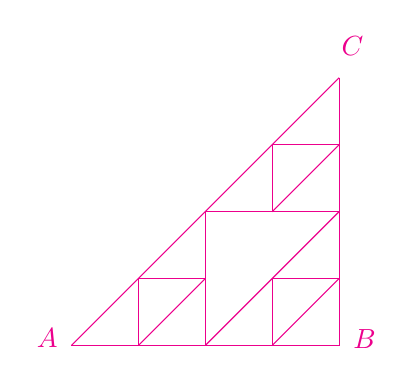
\begin{tikzpicture}[toancuabi,scale=0.85]
			\draw  (-4.,0.)-- (0.,0.);
			\draw  (0.,4.)-- (0.,0.);
			\draw  (0.,4.)-- (-4.,0.);
			\draw  (-3.,0.)-- (-3.,1.);
			\draw  (-3.,1.)-- (-2.,1.);
			\draw  (-2.,0.)-- (-2.,2.);
			\draw  (-2.,2.)-- (0.,2.);
			\draw  (-1.,2.)-- (-1.,3.);
			\draw  (-1.,3.)-- (0.,3.);
			\draw  (0.,1.)-- (-1.,1.);
			\draw  (-1.,1.)-- (-1.,0.);
			\draw  (0.,2.)-- (-2.,0.);
			\draw  (0.,1.)-- (-1.,0.);
			\draw  (-2.,1.)-- (-3.,0.);
			\draw  (0.,3.)-- (-1.,2.);
			\draw (-4.36,0.11) node {$A$};
			\draw (0.38,0.09) node {$B$};
			\draw (0.2,4.47) node {$C$};
		\end{tikzpicture}
		\vspace*{-20pt}
	\end{wrapfigure}
	Sơ đồ dưới đây gồm nhiều tam giác vuông cân.
	\vskip 0.1cm
	Có bao nhiêu cách một con kiến có thể đi từ $A$ đến $C$ nếu nó chỉ được phép di chuyển lên trên, sang phải hay theo đường chéo? 
\vskip 0.1cm
\textbf{\color{toancuabi}Phân tích bài toán:} Tại mỗi điểm nút trên hình vẽ, số cách đi từ $A$ đến nó sẽ bằng tổng số cách đi từ $A$ đến các điểm nút ngay đằng trước nó theo chiều mũi tên được phép đi (phải, lên trên và đi chéo).
\vskip 0.1cm
	\begin{wrapfigure}{l}{0.5\linewidth}
		\centering
		\vspace*{-20pt}
		\captionsetup{labelformat=empty, justification=centering}
		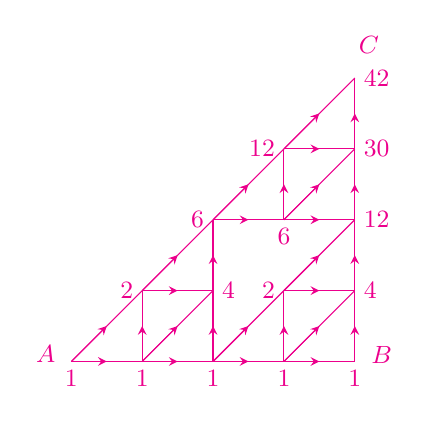
\begin{tikzpicture}[toancuabi,scale=0.9,node font=\small]
			\draw  (-4.,0.)-- (0.,0.);
			\draw  (0.,4.)-- (0.,0.);
			\draw  (0.,4.)-- (-4.,0.);
			\draw  (-3.,0.)-- (-3.,1.);
			\draw  (-3.,1.)-- (-2.,1.);
			\draw  (-2.,0.)-- (-2.,2.);
			\draw  (-2.,2.)-- (0.,2.);
			\draw  (-1.,2.)-- (-1.,3.);
			\draw  (-1.,3.)-- (0.,3.);
			\draw  (0.,1.)-- (-1.,1.);
			\draw  (-1.,1.)-- (-1.,0.);
			\draw  (0.,2.)-- (-2.,0.);
			\draw  (0.,1.)-- (-1.,0.);
			\draw  (-2.,1.)-- (-3.,0.);
			\draw  (0.,3.)-- (-1.,2.);
			
			\draw[-stealth]  (-4.,0.)-- (-3.5,0.);
			\draw[-stealth]  (-3.,0)-- (-2.5,0.);
			\draw[-stealth]  (-2,0)-- (-1.5,0.);
			\draw[-stealth] (-1.,0.)-- (-0.5,0.);
			\draw[-stealth]  (0,0)-- (0,0.5);
			\draw[-stealth]  (0,1)-- (0,1.5);
			\draw[-stealth]  (0,2)-- (0,2.5);
			\draw[-stealth]  (0,3)-- (0,3.5);
			\draw[-stealth]  (-3,1)-- (-2.5,1);
			\draw[-stealth]  (-1,1)-- (-0.5,1);
			\draw[-stealth]  (-2,2)-- (-1.5,2);
			\draw[-stealth]  (-1,2)-- (-0.5,2);
			\draw[-stealth]  (-1,3)-- (-0.5,3);
			
			\draw[-stealth]  (-4,0)-- (-3.5,0.5);
			\draw[-stealth]  (-3,1)-- (-2.5,1.5);
			\draw[-stealth]  (-2.,2.)-- (-1.5,2.5);
			\draw[-stealth]  (-1.,3.)-- (-0.5,3.5);
			\draw[-stealth]  (-3,0)-- (-2.5,0.5);
			\draw[-stealth]  (-2,0)-- (-1.5,0.5);
			\draw[-stealth]  (-1,0)-- (-0.5,0.5);
			\draw[-stealth]  (-1,1)-- (-0.5,1.5);
			\draw[-stealth]  (-1,2)-- (-0.5,2.5);
			
			\draw[-stealth]  (-3,0)-- (-3,0.5);
			\draw[-stealth]  (-2,0)-- (-2,.5);
			\draw[-stealth]  (-1,0)-- (-1,0.5);
			\draw[-stealth]  (-2,1)-- (-2,1.5);
			\draw[-stealth]  (-1,2)-- (-1,2.5);
			
			\draw (-4.36,0.11) node {$A$};
			\draw (0.38,0.09) node {$B$};
			\draw (0.2,4.47) node {$C$};
			
			\draw (-4,0) node[below]{$1$};
			\draw (-3,0) node[below]{$1$};
			\draw (-2,0) node[below] {$1$};
			\draw (-1,0) node[below] {$1$};
			\draw (0,0) node[below] {$1$};
			\draw (-3,1) node[left] {$2$};
			\draw (-2,1) node[right] {$4$};
			\draw (-1,1) node[left] {$2$};
			\draw (0,1) node[right] {$4$};
			\draw (-2,2) node[left] {$6$};
			\draw (-1,2) node[below] {$6$};
			\draw (0,2) node[right] {$12$};
			\draw (0,3) node[right] {$30$};
			\draw (0,4) node[right] {$42$};
			\draw (-1,3) node[left] {$12$};
		\end{tikzpicture}
		\vspace*{-20pt}
	\end{wrapfigure}
	\vskip 0.1cm
	Vậy nên ta có thể điền mũi tên hướng đi và áp dụng quy tắc cộng để giải quyết các bài toán dạng này.
	\vskip 0.1cm
	\textit{Lời giải}: Theo quy tắc cộng thể hiện trên hình vẽ bên dưới ta có tổng số cách đi từ $A$ đến $C$ là $42$.
	\vskip 0.1cm
\textbf{\color{toancuabi}Bài toán số $\pmb2$: (IMAS)}
\vskip 0.1cm
$8$ ký tự $2,0,1,5,I,M,A,S$ được xếp trên $1$ hàng. Hỏi có bao nhiêu cách xếp sao cho các chữ số đứng đằng trước các chữ cái, chữ số $0$ không đứng đầu tiên.
\vskip 0.1cm
\textit{Lời giải.}
Có $8$ vị trí để xếp $8$ ký tự, các chữ số đứng đằng trước các chữ cái nên $4$ vị trí đầu tiên là các chữ số và $4$ vị trí sau cùng. Ta thực hiện $2$ công việc là xếp chữ số và xếp chữ cái:
\vskip 0.1cm
+ Có $3\times3\times2\times1=18$ cách xếp các chữ số (chữ số $0$ không đứng ở đầu nên vị trí đầu chỉ có $3$ cách chọn chữ số).
\vskip 0.1cm
+ Có $4\times3\times2\times1=4!=24$ cách xếp $4$ chữ cái.
\vskip 0.1cm
Theo quy tắc nhân (hai quy tắc cơ bản trong đếm tổ hợp là quy tắc cộng và quy tắc nhân) ta có số cách xếp $8$ ký tự là: $18\times24=432$.
\vskip 0.1cm
(Ta có thể lập luận: ta thực hiện $3$ công việc theo thứ tự là Job $1$ là viết chữ số đầu tiên, Job $2$ là viết $3$ chữ số tiếp theo, Job $3$ là viết $4$ chữ cái, và theo quy tắc nhân ta có kết quả là: $P(3,1)\times P(3,3)\times P(4,4)=3\times3!\times4!=432$)
\vskip 0.1cm
Mở rộng bài toán số $2$, các bạn thử sức với bài toán số $3$ nhé.
\vskip 0.1cm
\textbf{\color{toancuabi}Bài toán số $3$:}
\vskip 0.1cm
$8$ ký tự $2,0,1,5,I,M,A,S$ được xếp trên $1$ hàng. Hỏi có bao nhiêu cách xếp thỏa mãn một trong các điều kiện sau:
\vskip 0.1cm
$a)$ Không có hai chữ cái nào đứng cạnh nhau.
\vskip 0.1cm
$b)$ Chữ số $0$ nằm giữa hai chữ cái $I$ và $S$.
\vskip 0.1cm
$c)$ Chữ số $0$ và chữ số $1$ không đứng cạnh nhau.
\vskip 0.1cm
$d)$ $4$ chữ cái luôn đứng cạnh nhau.
\vskip 0.1cm
\textbf{\color{toancuabi}Bài toán số $4$: (IMAS)}
\vskip 0.1cm
Có bao nhiêu số có $3$ chữ số không chứa chữ số $3$ và chia hết cho $3$.
\vskip 0.1cm
\textbf{\color{toancuabi}Phân tích bài toán:}
\vskip 0.1cm
Gọi số có $3$ chữ số là $\overline{abc}$:
\begin{multicols}{2}
	Thử từ số nhỏ để tìm quy luật:
	\begin{align*}
		&102, 105, 108\\
		&111, 114, 117\\
		&120, 126, 129\\
		&132, 135, 138\\
		&141, 144, 147\\
		&150, 156, 159...
	\end{align*}
	Ta nhận thấy chữ số $c$ lặp theo nhóm $(2,5,8)$, $(1,4,7)$, $(0,6,9)$ và mỗi nhóm này xuất hiện phụ thuộc vào số dư chi $3$ của số $\overline{ab}$ từ đó ta có lời giải như sau:
\vskip 0.1cm
\textit{Lời giải}
\vskip 0.1cm
Nếu $\overline{ab}$ chia $3$ dư $0$ ta có $3$ cách chọn $c=\{0,6,7\}$
\vskip 0.1cm
Nếu $\overline{ab}$ chia $3$ dư $1$ ta có $3$ cách chọn $c=\{2,5,8\}$
\vskip 0.1cm
Nếu $\overline{ab}$ chia $3$ dư $2$ ta có $3$ cách chọn $c=\{1,4,7\}$
\vskip 0.1cm
Vậy mỗi số $\overline{ab}$ ta luôn có $3$ cách chọn chữ số $c$.
\vskip 0.1cm
Ta có $9\times 10$ cách tạo ra số $\overline{ab}$.
\vskip 0.1cm
Vậy số số có $3$ chữ số không chứa chữ số $3$ và chia hết cho $3$ là: $9\times10\times3=270$ (số);
\end{multicols}
\vskip 0.1cm
\textbf{\color{toancuabi}Bài toán số $\pmb 5$: (APMOPS)}
\vskip 0.1cm
Mỗi cạnh của hình ngũ giác có cạnh $a,b,c,d,e$ tương ứng được tô bằng một trong $3$ mầu xanh, đỏ, vàng. Hỏi có bao nhiêu cách tô mầu cách cạnh của hình ngũ giác này sao cho không có $2$ cạnh nào kề nhau có cùng mầu.
\begin{multicols}{2}
	\begin{figure}[H]
		\centering
		\vspace*{-10pt}
		\captionsetup{labelformat=empty, justification=centering}
		\begin{tikzpicture}[toancuabi, scale=0.75]
			\draw  (-5.,3.)-- (-3.,4.);
			\draw  (-3.,4.)-- (-1.,4.);
			\draw  (-1.,4.)-- (0.,2.);
			\draw  (0.,2.)-- (-3.,0.);
			\draw  (-3.,0.)-- (-5.,3.);
			\draw (-4.08,3.89) node {$e$};
			\draw (-2.,4.35) node {$a$};
			\draw (-0.32,3.21) node {$b$};
			\draw (-1.2,0.95) node {$c$};
			\draw (-4.2,1.39) node {$d$};
		\end{tikzpicture}
		\vspace*{-10pt}
	\end{figure}
	\textbf{\color{toancuabi}Phân tích bài toán:} Nếu ta tô thứ tự $a,b,c,d,e$ thì $a$ và $b$ có tương ứng $3$ và $2$ cách tô. Đến tô $c$ thông thường sẽ có $2$ cách tô, $d$ cũng $2$ cách tô, nhưng nếu như vậy thì $e$ sẽ không xác định được số cách tô vì nó phụ thuộc vào $2$ cạnh $a$ và $d$, bởi vậy ta cần xét đến mầu cụ thể của $c$ cũng như của $d$ để tính được số cách tô mầu $c$. Vậy ta có thể tiếp cận bài toán bằng hai cách sau đây.
\vskip 0.1cm
\textit{Lời giải $1$:}
\vskip 0.1cm
Tô $a$, có $3$ cách tô, tô $b$, có $2$ cách tô.
\vskip 0.1cm
Tô $c$:
\vskip 0.1cm
\textbf{\color{toancuabi}Trường hợp $\pmb1$:} $c$ cùng mầu với $a, c$ có $1$ cách tô, $d$ có $2$ cách tô, $e$ có $1$ cách tô, số cách tô ngũ giác là: $3\times2\times1\times2\times1=12$ ($1$).
\vskip 0.1cm
\textbf{\color{toancuabi}Trường hợp $\pmb2$:} $c$ khác mầu với $a, c$ có $1$ cách tô (vì $c$ khác với cạnh $b$ kề với nó), xét $2$ khả năng tô $d$:
\vskip 0.1cm
$2.1$ $d$ cùng mầu với $a, d$ có $1$ cách tô, e có $2$ cách tô. Số cách tô ngũ giác là $3\times2\times1\times2\times1=12$ ($2$).
\vskip 0.1cm
$2.2$ $d$ khác mầu $a, d$ có $1$ cách tô (vì $c$ khác mầu $a$), $e$ có $1$ cách tô. Số cách tô ngũ giác là: $3\times2\times1\times1\times1=6$ ($3$).
\vskip 0.1cm
Từ ($1$),($2$),($3$) ta có số cách tô cần tìm là: $12+12+6=30$.
\end{multicols}
\textit{Lời giải $2$:}
\vskip 0.1cm
Tô $a$, có $3$ cách tô. Tô $c$, xét $2$ trường hợp:
\vskip 0.1cm
\textbf{\color{toancuabi}Trường hợp $\pmb1$:} $c$ cùng mầu $a, c$ có $1$ cách tô, $b$ có $2$ cách tô, $d$ có $2$ cách tô, $e$ có $1$ cách tô. Số cách tô ngũ giác là: $3\times1\times2\times2\times1=12$ ($1$).
\vskip 0.1cm
\textbf{\color{toancuabi}Trường hợp $\pmb2$:} $c$ khác mầu $a, c$ có $2$ cách tô, $b$ có $1$ cách tô. Xét $2$ khả năng tô $d$.
\vskip 0.1cm
$2.1$ $d$ cùng mầu với $a, d$ có $1$ cách tô, $e$ có $2$ cách tô. Số cách tô ngũ giác là: $3\times2\times1\times1\times2=12$ ($2$).
\vskip 0.1cm
$2.2$ $d$ khác mầu $a$, $d$ có $1$ cách tô (do $c$ khác mầu $a$), $e$ có $1$ cách tô. Số cách tô ngũ giác là: $3\times2\times1\times1\times1=6$ ($3$).
\vskip 0.1cm
Từ ($1$),($2$),($3$) ta có số cách tô cần tìm là: $12+12+6=30$.
\vskip 0.1cm
	\textbf{\color{toancuabi}Bài toán số $\pmb6$: (Apmops)}
	\vskip 0.1cm
	\begin{wrapfigure}{r}{0.4\linewidth}
		\centering
		\vspace*{-25pt}
		\captionsetup{labelformat=empty, justification=centering}
		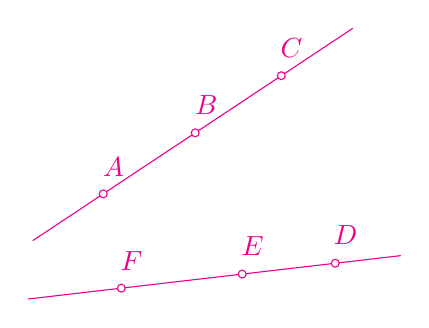
\begin{tikzpicture}[toancuabi,scale=0.95]
			\draw  (-5.,2.)-- (-0.02,2.58);
			\draw  (-4.94,2.78)-- (-0.66,5.62);
			\draw[fill=white]  (-3.9971801091570645,3.4056094602789573) circle (1.5pt);
			\draw (-3.86,3.77) node {$A$};
			\draw[fill=white]  (-2.7676858702243776,4.221442086112797) circle (1.5pt);
			\draw (-2.62,4.59) node {$B$};
			\draw[fill=white]  (-1.6167058823529414,4.985176470588236) circle (1.5pt);
			\draw (-1.48,5.35) node {$C$};
			\draw[fill=white]  (-3.7559113331848124,2.144893860793737) circle (1.5pt);
			\draw (-3.62,2.51) node {$F$};
			\draw[fill=white]  (-2.1392062633270745,2.3331848127048787) circle (1.5pt);
			\draw (-2.,2.71) node {$E$};
			\draw[fill=white]  (-0.8951175965118869,2.4780786734986155) circle (1.5pt);
			\draw (-0.76,2.85) node {$D$};
		\end{tikzpicture}
		\vspace*{-15pt}
	\end{wrapfigure}
	\vskip 0.1cm
	$A,B,C,D,E$ và $F$ là các điểm nằm trên $2$ đường thẳng như hình vẽ. Có bao nhiêu tam giác được tạo bởi $3$ trong $6$ điểm đã cho.
	\vskip 0.1cm
\textbf{\color{toancuabi}Phân tích bài toán:}
\vskip 0.1cm
Trên mặt phẳng cứ $3$ điểm phân biệt không thẳng hàng luôn tạo ra một tam giác, còn $3$ điểm phân biệt thẳng hàng thì không tạo ra một tam giác thông thường mà thường được gọi là tam giác suy biến (degenerate triangle). Tương tự như thế, nếu có các đường thẳng đôi một cắt nhau, mà không có $3$ đường thẳng nào cắt nhau tại $1$ điểm ($3$ đường đồng quy) thì cứ $3$ đường thẳng tạo ra được $1$ đoạn thẳng. Cứ $3$ đường thẳng đồng quy thì nó tạo ra một tam giác suy biến (có $3$ đỉnh trùng vào nhau). Các tính chất này có thể được áp dụng để giải bài toán trên và các bài toán mở rộng ở phần dưới.
\vskip 0.1cm
\textit{Lời giải $1$:}
\vskip 0.1cm
Xét $2$ trường hợp, trường hợp $1$: tam giác có đáy nằm ở đường thẳng phía dưới, đỉnh nằm ở đường thẳng phía trên, có $C(3,2)$ cách chọn đáy và $C(3,1)$ cách chọn đỉnh, theo quy tắc nhân, số tam giác đếm được là: $C(3,2)\times C(3,1)$. Tương tự, trường hợp $2$: tam giác có đáy nằm ở đường thẳng phía trên, đỉnh nằm ở đường thẳng phía dưới, có $C(3,2)$ cách chọn đáy và $C(3,1)$ cách chọn đỉnh, theo quy tắc nhân, số tam giác đếm được là: $C(3,2)\times C(3,1)$.
\vskip 0.1cm
Vậy số tam giác cần tìm là: $2\times C(3,2)\times C(3,1) = 2\times3\times3=18$.
\vskip 0.1cm
\textit{Lời giải $2$:}
\vskip 0.1cm
Số cách chọn ra $3$ điểm là: $C(6,3)=6\times 5\times4/3!=20$
\vskip 0.1cm
Số tam giác suy biến là: $3\times C(3,3)=2$
\vskip 0.1cm
Vậy số tam giác là: $20-2=18$
\vskip 0.1cm
Mở rộng bài toán số $5$, các bạn thử sức của mình xem sao nhé.
\vskip 0.1cm
	\textbf{\color{toancuabi}Bài toán $\pmb{6.1}$ (Apmops)}
	\vskip 0.1cm
	\begin{wrapfigure}{r}{0.5\linewidth}
		\centering
		\vspace*{-5pt}
		\captionsetup{labelformat=empty, justification=centering}
		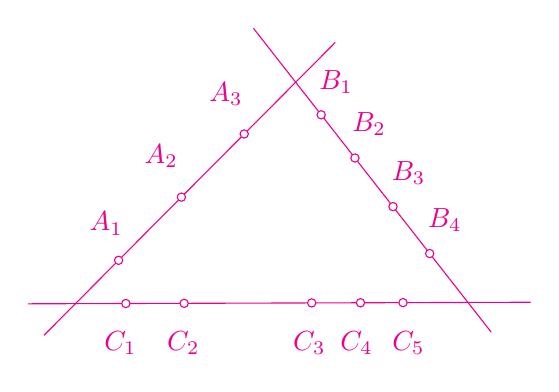
\begin{tikzpicture}[toancuabi, scale=1]
			\draw  (-5.4,1.6)-- (-1.7,5.32);
			\draw  (-2.74,5.5)-- (0.28,1.64);
			\draw  (-5.6,2.)-- (0.78,2.02);
			\draw[fill=white]  (-4.45248688627018,2.552634806236469) circle (1.5pt);
			\draw (-4.61,3.02) node {$A_1$};
			\draw[fill=white]  (-3.6547027796748095,3.3547312593539766) circle (1.5pt);
			\draw (-3.91,3.88) node {$A_2$};
			\draw[fill=white]  (-2.856811147760132,4.1569358190087335) circle (1.5pt);
			\draw (-3.09,4.66) node {$A_3$};
			\draw[fill=white]  (-1.8796143213988348,4.400301748542881) circle (1.5pt);
			\draw (-1.69,4.82) node {$B_1$};
			\draw[fill=white]  (-1.4504776019983348,3.851802497918401) circle (1.5pt);
			\draw (-1.27,4.28) node {$B_2$};
			\draw[fill=white]  (-0.9673278934221485,3.2342667776852623) circle (1.5pt);
			\draw (-0.77,3.66) node {$B_3$};
			\draw[fill=white]  (-0.5014784346378021,2.6388432972522895) circle (1.5pt);
			\draw (-0.31,3.06) node {$B_4$};
			\draw[fill=white]  (-4.359949489986439,2.003887305674024) circle (1.5pt);
			\draw (-4.43,1.5) node {$C_1$};
			\draw [fill=white] (-3.619831371238773,2.0062074251685305) circle (1.5pt);
			\draw (-3.63,1.5) node {$C_2$};
			\draw[fill=white]  (-2.0000353766631944,2.0112851555590496) circle (1.5pt);
			\draw (-2.03,1.5) node {$C_3$};
			\draw[fill=white]  (-1.3800414693107446,2.0132287101275526) circle (1.5pt);
			\draw (-1.43,1.5) node {$C_4$};
			\draw[fill=white]  (-0.839921385192901,2.0149218765354453) circle (1.5pt);
			\draw (-0.77,1.5) node {$C_5$};
		\end{tikzpicture}
		\vspace*{-25pt}
	\end{wrapfigure}
	Cho các điểm $A1$, $A2$, $A3$, $B1$, $B2$, $B3$, $B4$, $C1$, $C2$, $C3$, $C4$ và $C5$ nằm trên $3$ đường thẳng như hình vẽ. Có bao nhiêu tam giác được tạo bởi $3$ trong các đỉnh đã cho?
	\vskip 0.1cm
	\textbf{\color{toancuabi}Bài toán $\pmb{6.2}$}
	Có bao nhiêu tam giác trong hình vẽ?
	\begin{figure}[H]
		\centering
		\vspace*{-10pt}
		\captionsetup{labelformat=empty, justification=centering}
		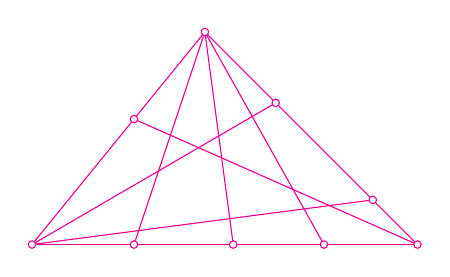
\begin{tikzpicture}[toancuabi,scale=0.9]
			\draw  (1.,3.)-- (-1.44,0.);
			\draw  (-1.44,0.)-- (4.,0.);
			\draw  (4.,0.)-- (1.,3.);
			\draw  (1.,3.)-- (0.,0.);
			\draw  (1.,3.)-- (1.4,0.);
			\draw  (1.,3.)-- (2.68,0.);
			\draw  (4.,0.)-- (0.,1.7704918032786887);
			\draw  (-1.44,0.)-- (2.,2.);
			\draw  (-1.44,0.)-- (3.37,0.63);
			\draw [fill=white] (1.,3.) circle (1.5pt);
			\draw [fill=white] (-1.44,0.) circle (1.5pt);
			\draw [fill=white] (4.,0.) circle (1.5pt);
			\draw [fill=white] (0.,0.) circle (1.5pt);
			\draw [fill=white] (1.4,0.) circle (1.5pt);
			\draw [fill=white] (2.68,0.) circle (1.5pt);
			\draw [fill=white] (0.,1.7704918032786887) circle (1.5pt);
			\draw [fill=white] (2.,2.) circle (1.5pt);
			\draw [fill=white] (3.37,0.63) circle (1.5pt);
		\end{tikzpicture}
		\vspace*{-5pt}
	\end{figure}
	\textbf{\color{toancuabi}Bài toán $\pmb{6.3}$}
	\vskip 0.1cm
	Có bao nhiêu tam giác được tạo bởi $3$ trong $12$ điểm đã cho trên lưới ô vuông như hình vẽ?
	\begin{figure}[H]
		\centering
		\vspace*{5pt}
		\captionsetup{labelformat=empty, justification=centering}
		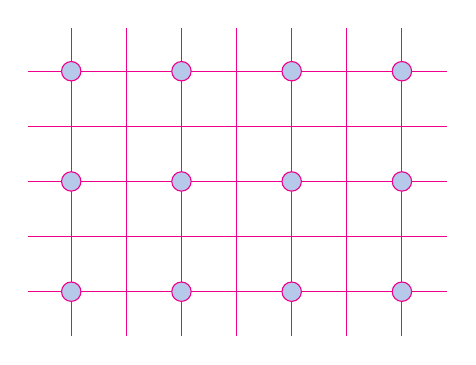
\begin{tikzpicture}[toancuabi,scale=0.7]
			\draw [xstep=1.0cm,ystep=1.0cm] (-2.78,-0.8) grid (4.82,4.78);
			\draw [fill=cackithi!40] (-2.,4.) circle (5.0pt);
			\draw [fill=cackithi!40] (0.,4.) circle (5.0pt);
			\draw [fill=cackithi!40] (2.,4.) circle (5.0pt);
			\draw [fill=cackithi!40] (4.,4.) circle (5.0pt);
			\draw [fill=cackithi!40] (4.,2.) circle (5.0pt);
			\draw [fill=cackithi!40] (4.,0.) circle (5.0pt);
			\draw [fill=cackithi!40] (2.,0.) circle (5.0pt);
			\draw [fill=cackithi!40] (2.,2.) circle (5.0pt);
			\draw [fill=cackithi!40] (0.,2.) circle (5.0pt);
			\draw [fill=cackithi!40] (0.,0.) circle (5.0pt);
			\draw [fill=cackithi!40] (-2.,2.) circle (5.0pt);
			\draw [fill=cackithi!40] (-2.,0.) circle (5.0pt);
		\end{tikzpicture}
		\vspace*{-5pt}
	\end{figure}
\vskip 0.1cm
\textbf{\color{toancuabi}Bài toán số $\pmb{7}$: (Apmops)}
\vskip 0.1cm
Có bao nhiêu cách để tô $6$ mặt của một hình lập phương bằng $6$ mầu, mỗi mặt được tô bằng $1$ mầu sao cho không có hai mặt nào có cùng mầu? (Hai cách tô mầu được coi là như nhau nếu chúng nhìn giống hệt nhau sau một phép xoay hình). 
\vskip 0.1cm
\textbf{\color{toancuabi}Phân tích bài toán:} Hướng đi thứ nhất, ta hình dung nếu cố định hình lập phương lại và mỗi cách nhìn khác nhau ở mỗi phía được coi là khác nhau, như thế thì số cách tô sẽ như tô theo hàng ngang ($6$ người ngồi trên $6$ cái ghế trên $1$ hàng) và sẽ là $6!=720$ cách. Do hình lập phương này xoay được nên ta xem mỗi một kiểu tô có bao nhiêu cách xoay nó xung quanh chính nó. Do có $6$ mầu ta có $6$ cách xoay để có đáy khác mầu. Mỗi cách đặt đáy với $1$ mầu ta có $4$ cách xoay xung quanh chính nó (do hình lập phương có $4$ cạnh bên), từ đó ta có hướng giải quyết bài toán.
\vskip 0.1cm
Hướng đi thứ $2$, do hình lập phương xoay được nên ta có thể cố định mầu ở những vị trí ta có thể xoay nó về và ta sẽ có hướng giải quyết bài toán như lời giải $2$.
\vskip 0.1cm
Hướng đi thứ $3$ gần giống với hướng thứ $2$, ta có thể hình dung mình có thể tô mầu ở đáy bằng mầu tùy thích do hình lập phương xoay được, mặt đối diện trên đỉnh sẽ còn $5$ cách tô, $4$ mặt xung quanh ta sẽ hình dung nó như $4$ người ngồi xung quanh một cái bàn tròn nên ta có thể áp dụng bài toán hoán vị vòng tròn để giải quyết.
\vskip 0.1cm
\textit{Lời giải $1$:}
\vskip 0.1cm 
Giả sử hình lập phương cố định, khi đó ta có $6!=720$ cách tô.
\vskip 0.1cm
Mỗi cách tô ta có $6$ cách đặt các mặt khác mầu nhau xuống đáy, khi đặt rồi ta có $4$ cách xoay xung quanh nó, vậy ứng với mỗi cách tô mầu ta có $6\times4=24$ cách xoay nó xung quanh chính nó. Vậy số cách tô mầu là: $720:24=30$ (cách).
\vskip 0.1cm
\textit{Lời giải $2$:}
\vskip 0.1cm 
Đầu tiên ta tô mầu $1$ mặt (mầu ta thích), rồi đặt nó xuống đáy, khi đó ở mặt đối diện trên đỉnh có $5$ cách tô.
\vskip 0.1cm
Tiếp theo ta tô mầu $1$ mặt xung quanh (mầu ta thích trong $4$ mầu còn lại), rồi xoay nó sang bên trái, khi đó mặt bên phải có $3$ cách tô, còn $2$ mặt còn lại (trước và sau) có $2!$ cách tô, vậy số cách tô mầu là: $1\times5\times1\times3\times2!=30$ (cách)
\vskip 0.1cm
\textit{Lời giải $3$:}
\vskip 0.1cm
Tương tự như lời giải $2$, đầu tiên ta tô mầu $1$ mặt (mầu ta thích), rồi đặt nó xuống đáy, khi đó ở mặt đối diện trên đỉnh có $5$ cách tô.
\vskip 0.1cm
Còn $4$ mặt xung quanh, do xoay được nên theo bài toán hoán vị vòng tròn ta có $4!/4=6$ cách tô.
\vskip 0.1cm
Vậy số cách tô mầu hình lập phương là: $5\times 6=30$ (cách).
\vskip 0.1cm
\textbf{\color{toancuabi}Bài toán số $\pmb8$: (IMSO)}
\vskip 0.1cm
Một hình lập phương được tô các mặt bằng $6$ mầu, mỗi mặt $1$ mầu khác nhau và được đánh số từ $1$ đến $6$ sao cho tổng hai mặt đối diện bằng $7$. Hỏi có bao nhiêu cách tô mầu và đánh số hình lập phương này? (Hai cách tô mầu, đánh số được coi là như nhau nếu chúng nhìn giống hệt nhau sau một phép xoay hình). 
\vskip 0.1cm
Phân tích bài toán: Bài toán này là tương đối khó khi các bạn lớp $5,6$ đi thi gặp phải, và đúng là trong năm thi đó đoàn học sinh Việt Nam chỉ có đúng $1$ bạn làm được, tuy nhiên nếu chia bài toán làm hai bước, bước $1$ tô mầu, bước $2$ điền số thì ta có thể giải quyết được bài toán một cách tương đối dễ dàng.
\vskip 0.1cm
\textit{Lời giải:}
\vskip 0.1cm 
Bước $1$: Tô mầu hình lập phương, theo bài toán số $7$, ta có $30$ cách tô mầu hình lập phương này.
\vskip 0.1cm
Bước $2$: Đánh số, ta đánh theo thứ tự:
\vskip 0.1cm
Đánh số $1$, có $6$ cách. Đánh số $6$ ở mặt đối diện số $1$, có $1$ cách.
\vskip 0.1cm
Đánh số $2$, có $4$ cách (do còn $4$ mặt chưa đánh số). Đánh số $5$ ở mặt đối diện, có $1$ cách.
\vskip 0.1cm
Đánh số $3$, có $2$ cách (do còn $2$ mặt chưa đánh số). Đánh số $4$ ở mặt đối diện, có $1$ cách.
\vskip 0.1cm
Vậy ta có $6\times1\times4\times1\times2\times1=48$ cách đánh số.
\vskip 0.1cm
Theo quy tắc nhân ta có số cách tô mầu và đánh số là: $30\times 48=1440$ (cách).
\vskip 0.1cm
	\textbf{\color{toancuabi}Bài toán số $\pmb9$: (IMAS)}
	\vskip 0.1cm
	\begin{wrapfigure}{r}{0.45\linewidth}
		\centering
		\vspace*{-15pt}
		\captionsetup{labelformat=empty, justification=centering}
		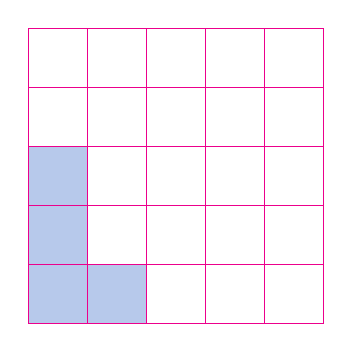
\begin{tikzpicture}[toancuabi,scale=0.75]
			\filldraw[cackithi!40] (0,0) rectangle (1,3);
			\filldraw[cackithi!40] (1,0) rectangle (2,1);
			\draw (0,0) grid (5,5);
		\end{tikzpicture}
		\vspace*{-10pt}
	\end{wrapfigure}
	Một bàn cờ hình vuông $5\times 5$ được xếp một hình chữ L chiếm $4$ ô như hình vẽ. Ta có thể xoay hoặc lật hình chữ L này. Hỏi có bao nhiêu cách xếp hình chữ L này vào bàn cờ hình vuông đã cho?
\vskip 0.1cm
Phân tích bài toán: Ta nhận thấy hình chữ L tô đen có thể xoay hoặc lật được, nên ta sẽ xem nó có thể có bao nhiêu cách biến hình (xoay hoặc lật).  Ứng với mỗi phép biến hình bằng xoay, lật ta xem có bao nhiêu cách trượt nó theo hàng ngang và hàng dọc, từ đó ta có cách giải quyết bài toán.
\vskip 0.1cm
\textit{Lời giải:}
\vskip 0.1cm
Ta tính số cách xoay, lật hình chữ L tô đậm, như hình dưới ta có $8$ cách.
	\begin{figure}[H]
		\centering
		\vspace*{-5pt}
		\captionsetup{labelformat=empty, justification=centering}
		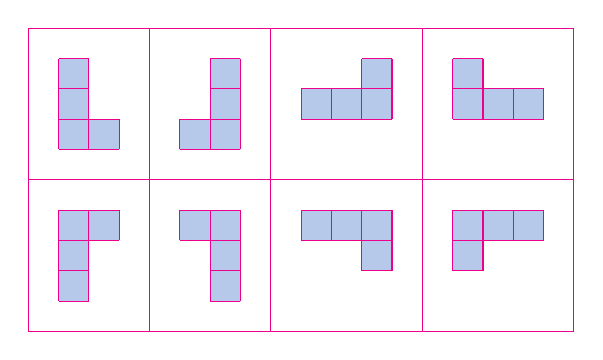
\begin{tikzpicture}[toancuabi,scale=0.385]
			\fill[cackithi!40] (1.,3.) -- (2.,3.) -- (2.,1.) -- (3.,1.) -- (3.,0.) -- (1.,0.) -- cycle;
			\fill[cackithi!40] (5.,0.) -- (7.,0.) -- (7.,3.) -- (6.,3.) -- (6.,1.) -- (5.,1.) -- cycle;
			\fill[cackithi!40] (9.,2.) -- (11.,2.) -- (11.,3.) -- (12.,3.) -- (12.,1.) -- (9.,1.) -- cycle;
			\fill[cackithi!40] (14.,3.) -- (14.,1.) -- (17.,1.) -- (17.,2.) -- (15.,2.) -- (15.,3.) -- cycle;
			\fill[cackithi!40] (3.,-2.) -- (1.,-2.) -- (1.,-5.) -- (2.,-5.) -- (2.,-3.) -- (3.,-3.) -- cycle;
			\fill[cackithi!40] (5.,-2.) -- (7.,-2.) -- (7.,-5.) -- (6.,-5.) -- (6.,-3.) -- (5.,-3.) -- cycle;
			\fill[cackithi!40] (9.,-2.) -- (12.,-2.) -- (12.,-4.) -- (11.,-4.) -- (11.,-3.) -- (9.,-3.) -- cycle;
			\fill[cackithi!40] (14.,-2.) -- (14.,-4.) -- (15.,-4.) -- (15.,-3.) -- (17.,-3.) -- (17.,-2.) -- cycle;
			\draw [] (1.,3.)-- (2.,3.);
			\draw [] (2.,3.)-- (2.,1.);
			\draw [] (2.,1.)-- (3.,1.);
			\draw [] (3.,1.)-- (3.,0.);
			\draw [] (3.,0.)-- (1.,0.);
			\draw [] (1.,0.)-- (1.,3.);
			\draw [] (5.,0.)-- (7.,0.);
			\draw [] (7.,0.)-- (7.,3.);
			\draw [] (7.,3.)-- (6.,3.);
			\draw [] (6.,3.)-- (6.,1.);
			\draw [] (6.,1.)-- (5.,1.);
			\draw [] (5.,1.)-- (5.,0.);
			\draw [] (9.,2.)-- (11.,2.);
			\draw [] (11.,2.)-- (11.,3.);
			\draw [] (11.,3.)-- (12.,3.);
			\draw [] (12.,3.)-- (12.,1.);
			\draw [] (12.,1.)-- (9.,1.);
			\draw [] (9.,1.)-- (9.,2.);
			\draw [] (14.,3.)-- (14.,1.);
			\draw [] (14.,1.)-- (17.,1.);
			\draw [] (17.,1.)-- (17.,2.);
			\draw [] (17.,2.)-- (15.,2.);
			\draw [] (15.,2.)-- (15.,3.);
			\draw [] (15.,3.)-- (14.,3.);
			\draw [] (3.,-2.)-- (1.,-2.);
			\draw [] (1.,-2.)-- (1.,-5.);
			\draw [] (1.,-5.)-- (2.,-5.);
			\draw [] (2.,-5.)-- (2.,-3.);
			\draw [] (2.,-3.)-- (3.,-3.);
			\draw [] (3.,-3.)-- (3.,-2.);
			\draw [] (5.,-2.)-- (7.,-2.);
			\draw [] (7.,-2.)-- (7.,-5.);
			\draw [] (7.,-5.)-- (6.,-5.);
			\draw [] (6.,-5.)-- (6.,-3.);
			\draw [] (6.,-3.)-- (5.,-3.);
			\draw [] (5.,-3.)-- (5.,-2.);
			\draw [] (9.,-2.)-- (12.,-2.);
			\draw [] (12.,-2.)-- (12.,-4.);
			\draw [] (12.,-4.)-- (11.,-4.);
			\draw [] (11.,-4.)-- (11.,-3.);
			\draw [] (11.,-3.)-- (9.,-3.);
			\draw [] (9.,-3.)-- (9.,-2.);
			\draw [] (14.,-2.)-- (14.,-4.);
			\draw [] (14.,-4.)-- (15.,-4.);
			\draw [] (15.,-4.)-- (15.,-3.);
			\draw [] (15.,-3.)-- (17.,-3.);
			\draw [] (17.,-3.)-- (17.,-2.);
			\draw [] (17.,-2.)-- (14.,-2.);
			\draw  (0.,4.)-- (18.,4.);
			\draw  (18.,4.)-- (18.,-6.);
			\draw  (18.,-6.)-- (0.,-6.);
			\draw  (0.,4.)-- (0.,-6.);
			\draw  (0.,-1.)-- (18.,-1.);
			\draw  (13.,4.)-- (13.,-6.);
			\draw  (8.,4.)-- (8.,-6.);
			\draw  (4.,4.)-- (4.,-6.);
			\draw  (1.,2.)-- (2.,2.);
			\draw  (1.,1.)-- (2.,1.);
			\draw  (2.,1.)-- (2.,0.);
			\draw  (6.,2.)-- (7.,2.);
			\draw  (6.,1.)-- (7.,1.);
			\draw  (6.,1.)-- (6.,0.);
			\draw  (11.,2.)-- (11.,1.);
			\draw  (10.,2.)-- (10.,1.);
			\draw  (11.,2.)-- (12.,2.);
			\draw  (15.,2.)-- (15.,1.);
			\draw  (15.,2.)-- (14.,2.);
			\draw  (16.,2.)-- (16.,1.);
			\draw  (15.,-2.)-- (15.,-3.);
			\draw  (16.,-2.)-- (16.,-3.);
			\draw  (15.,-3.)-- (14.,-3.);
			\draw  (11.,-3.)-- (12.,-3.);
			\draw  (11.,-3.)-- (11.,-2.);
			\draw  (10.,-2.)-- (10.,-3.);
			\draw  (6.,-3.)-- (7.,-3.);
			\draw  (7.,-4.)-- (6.,-4.);
			\draw  (6.,-3.)-- (6.,-2.);
			\draw  (2.,-3.)-- (2.,-2.);
			\draw  (2.,-3.)-- (1.,-3.);
			\draw  (1.,-4.)-- (2.,-4.);
		\end{tikzpicture}
		\vspace*{-10pt}
	\end{figure}
Ứng với mỗi cách biến hình này, ta xem có bao nhiêu cách dời hình theo hàng ngang và hàng dọc, và ta tính được số cách dời hình bằng trượt (tịnh tiến) theo hai chiều ngang, dọc là: $3\times4=12$.
\vskip 0.1cm
		\begin{figure}[H]
			\centering
			\vspace*{-5pt}
			\begin{tikzpicture}[toancuabi,scale=0.62, node font= \scriptsize]
				\filldraw[cackithi!40] (0,0) rectangle (1,3);
				\filldraw[cackithi!40] (1,0) rectangle (2,1);
				\draw (0,0) grid (5,5);
				\draw (1.5,0.5) node {$1$};
				\draw (2.5,0.5) node {$2$};
				\draw (3.5,0.5) node {$3$};
				\draw (4.5,0.5) node {$4$};
				\draw (0.5,2.5) node {$1$};
				\draw (0.5,3.5) node {$2$};
				\draw (0.5,4.5) node {$3$};			
				\draw (0.2, 5.5) node[right] {$3$ cách di chuyển theo cột dọc};
				\draw (5.2, 0.4) node[right] {$4$ cách di chuyển theo hàng ngang};
			\end{tikzpicture}
			\vspace*{-5pt}
		\end{figure}
	Theo quy tắc nhân, ta có số cách đặt chữ L vào ô vuông $5\times 5$ là: $8\times12=96$ (cách)
\vskip 0.1cm
Mở rộng bài toán số $9$. Các bạn thử sức mình xem nhé.
\vskip 0.1cm
\textbf{\color{toancuabi}Bài toán số $\pmb{9.1}$}: Đề bài giống như bài toán số $9$, hình được xếp vào được thay đổi như sau:
	\begin{figure}[H]
		\centering
		\vspace*{-5pt}
		\captionsetup{labelformat=empty, justification=centering}
		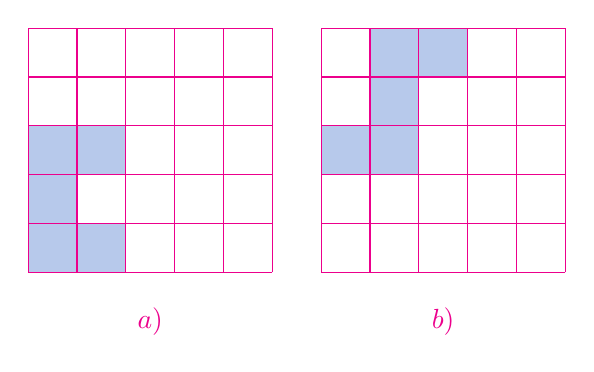
\begin{tikzpicture}[toancuabi,scale=0.62]
			\filldraw [cackithi!40] (0,0) rectangle (1,3);
			\filldraw [cackithi!40] (1,0) rectangle (2,1);
			\filldraw [cackithi!40] (1,2) rectangle (2,3);
			\filldraw [cackithi!40] (6,2) rectangle (8,3);
			\filldraw [cackithi!40] (7,3) rectangle (8,5);
			\filldraw [cackithi!40] (8,4) rectangle (9,5);
			\draw (0,0) grid (5,5);
			\draw (6,0) grid (11,5);
			\draw (2.5, -1) node {$a)$};
			\draw (8.5, -1) node {$b)$};
		\end{tikzpicture}
		\vspace*{-5pt}
	\end{figure}
\textbf{\color{toancuabi}Bài toán số $\pmb{10}$: (IMSO).}
\vskip 0.1cm
Một hình tròn và một tam giác được xếp trên các điểm cắt của lưới ô vuông như hình vẽ sao cho tam giác và hình tròn không cùng nằm trên một hàng hay một cột.
\vskip 0.1cm
	Hỏi có bao nhiêu cách xếp tam giác và hình tròn vào lưới ô vuông như hình vẽ này. Trên hình vẽ là một ví dụ về cách xếp tam giác và hình tròn.
	\begin{figure}[H]
		\centering
		\vspace*{-10pt}
		\captionsetup{labelformat=empty, justification=centering}
		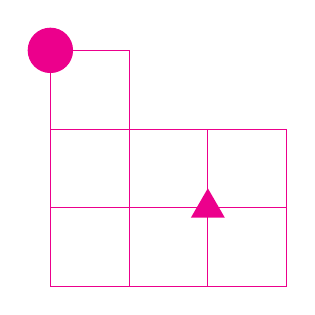
\begin{tikzpicture}[scale= 1,toancuabi]
			\draw (0,0) grid (3,2);
			\draw (0,2) grid (1,3);
			\draw[fill = toancuabi] (0,3) circle (8pt);
%			\node[fill=white, toancuabi, inner sep=2.5pt] at (2,1) {};
			\node[fill=white, toancuabi,regular polygon, regular polygon sides=3,inner sep=2.5pt] at (2,1) {};
		\end{tikzpicture}
		\vspace*{-10pt}
	\end{figure}
\vskip 0.1cm
\textbf{\color{toancuabi}Phân tích bài toán:} Bài toán này các bạn nhỏ lớp $4,5$ trong câu lạc bộ toán UMC đã làm được theo nhiều cách khác nhau, các bạn quan sát sẽ thấy ngoài hai điểm ở hàng trên cùng thi bên dưới cứ mỗi hình chữ nhật sẽ có $2!\times 2!=4$ cách đặt hình tròn và tam giác (do mỗi cặp đỉnh không kề nhau của $1$ hình chữ nhật sẽ có $2!$ cách đặt hình tròn và tam giác). Sau đây là một số cách giải của các bạn.
\vskip 0.1cm
\textit{Lời giải $1$: }(Lê Kỳ Nam, Vĩnh Giang)
\vskip 0.1cm
Nếu đường tròn nằm trên hàng đầu tiên (có $2$ vị trí), thì ở mỗi vị trí sẽ có $14 - 4 - 1 = 9$ cách chọn tam giác, tổng số cách chọn là: $9 \times 2 = 18$.
\vskip 0.1cm
Nếu đường tròn đi vào phần còn lại của $2$ cột đầu tiên, thì ở mỗi vị trí, số cách chọn tam giác là $14 - 3 - 3 - 1 = 7$, tổng số cách chọn là $6 \times 7 = 42$.
\vskip 0.1cm
Nếu đường tròn đi ở $2$ cột cuối cùng, thì ở mỗi vị trí, tam giác sẽ có $14 - 3 - 2 - 1 = 8$ lựa chọn, tổng số cách chọn là $6 \times 8 = 48$.
\vskip 0.1cm
Tổng số cách xếp hình tròn và hình tam giác là: $18 + 42 + 48 = 108$.
\vskip 0.1cm
Đáp số: $108$
\vskip 0.1cm
\textit{Lời giải $2$:} (Nguyễn Gia Tuấn)
\vskip 0.1cm
Nếu hình tròn và hình tam giác không được đặt trên hình vuông trên cùng thì có $3 \times 4 \times 2 \times 3 = 72$ cách chọn.
\vskip 0.1cm
Nếu một trong các tam giác hoặc hình tròn được đặt trên hình vuông trên cùng thì có $2 \times 3 \times 3 \times 2 = 36$ cách chọn.
\vskip 0.1cm
Tổng cộng có $72 + 36 = 108$ cách chọn.
\vskip 0.1cm
\textit{Lời giải $3$:} (Nguyễn Trọng Cường).
\vskip 0.1cm
Tổng số các cách có thể đặt hình tròn và tam giác vào $2$ điểm bất kỳ của hình là: $14\times13 = 182$ cách
\vskip 0.1cm
Nếu hình tròn và tam giác nằm trên cùng $1$ cột, hoặc $1$ hàng, thì $2$ điểm sẽ tạo nên $1$ đoạn thẳng. Ta đếm số đoạn thẳng của hình trên.
\vskip 0.1cm
Số đoạn thẳng của hình là :
\begin{align*}
	1 + (1+2+3) \times 3 + (1+2+3) \times 2 + (1+2) \times 2 = 37
\end{align*}
Hình tròn và tam giác ở $2$ đầu đoạn thẳng, đổi chỗ được cho nhau $\Rightarrow$ có $37 \times 2 = 74$ cách ko thỏa mãn
\vskip 0.1cm
Số cách thỏa mãn đề bài là $182 - 74 = 108$ cách.
\vskip 0.1cm
\textit{Lời giải $4$:} (Nguyễn Gia Tuấn). -- Dùng phần bù:
\vskip 0.1cm
Với lưới ô vuông $3 \times 3$ thì ta có $C(4,2)\times C(4,2)\times 4 = 144$ cách chọn. (Do mỗi hình chữ nhật có $4$ cách đặt tam giác và hình tròn).
\vskip 0.1cm
Trong lưới $3 \times 3$ đó, nếu đặt hình tròn hoặc tam giác vào $2$ điểm trên cùng ở bên phải thì có $2 \times 3 \times  3 \times 2 = 36$ cách chọn.
\vskip 0.1cm
Vậy ta có $144 - 36 = 108$ cách chọn để xếp hình tròn và hình tam giác.
\vskip 0.1cm
Trả lời: $108$ lựa chọn.
	\newpage

	\thispagestyle{empty}
	\begingroup 
	\AddToShipoutPicture*{\put(0,0){\includegraphics[width=17.2cm]{../dovui/Do_vui_Pi11_2019}}}
	\centering
	\vspace*{0cm}
	\endgroup
	\newpage	

	\thispagestyle{empty}
	\begingroup 
	\AddToShipoutPicture*{\put(0,0){\includegraphics[width=17.2cm]{../dovui/Do_vui_Pi4_2020}}}
	\centering
	\vspace*{0cm}
	\endgroup
	\newpage
	
	\thispagestyle{empty}
	\begin{center}
		\textbf{\Large\color{toancuabi}PHẦN VII. LỜI GIẢI, ĐÁP ÁN}
	\end{center}
	\newpage	
	\graphicspath{{../loigiai/pic/}}

\begin{center}
	\textbf{\color{toancuabi}ĐÁP ÁN CÁC BÀI TOÁN TRONG MỤC \\ CHƠI CÙNG BI}
\end{center}
%\newpage
\begin{center}
	\textbf{\color{toancuabi}Đáp án bài toán trong Bài $\pmb3$ xếp hình nam châm}
\end{center}
Câu hỏi $5$
\vskip 0.1cm
$a.$	Tương tự câu $2$, bằng cách chia hình ra $4$ tầng ta đếm được số bi ở mỗi tầng là: $1,3,6,10$. Tổng số bi trong Hình $13$ là:
$$1+3+6+10= 20 \;(\text{viên}).$$
Hình $13$ tạo bởi $10$ kim tự tháp mà mỗi cạnh là một thanh đen. Số thanh đen là: 
$$10\times 6=60 \;(\text{thanh}).$$

$b.$	Tương tự câu $4$ ta lần lượt đếm được có $36$ tam  giác cạnh $1$, $20$ tam giác cạnh $2$, và $4$ tam giác cạnh $3$. Vậy tổng số tam giác có cạnh là các thanh đen là:
$$36+20+4=60  \;(\text{tam giác}).$$
\begin{center}
	\textbf{\color{toancuabi}Đáp án bài toán trong Bài 4 Triomino}
\end{center}
Câu hỏi $4$
\vskip 0.1cm
Chúng ta thấy rằng để có “trận đồ” ở Hình $19$, hai bạn Pi và Bi đã dùng hết các quân có đúng $2$ số $0$, và các quân có đúng hai số $1$. Ngoài ra, cho dù chơi tiếp thế nào sẽ không thể dùng quân gồm $3$ số $0$ và quân gồm $3$ số $1$ để chơi tiếp. Do vậy hai bạn không bao giờ có thể hết quân trên tay. “Trận đấu” này chắc chắn sẽ kết thúc với tình huống $2$.
\newpage
%===============
\newpage
\begin{center}
	\textbf{\color{toancuabi}ĐÁP ÁN CÁC BÀI TOÁN TRONG MỤC\\GIẢI TOẢN CÙNG BI}
\end{center}
\begin{center}
	\textbf{\color{toancuabi}Đáp án các bài toán trong Bài $\pmb5$ Robin và những hòn đảo bí ẩn}
\end{center}
Đáp án Câu hỏi $4$
\vskip 0.1cm
Để đếm được số chú ếch ở trên bờ và số chú ếch ở dưới ao, chúng ta cần phân biệt được hai miền: mặt ao và bờ ao. Do đó, số màu cần dùng để tô sẽ là một. Tiếp theo, do khóm sen nằm trên mặt ao nên để tô được mặt ao, ta cần đặt bút màu vào nơi có khóm sen trong Hình $1$, rồi tô màu sao cho trong quá trình tô, bút màu không rê qua đường viền đen ở bất cứ chỗ nào. Bằng cách đó, chúng ta sẽ thu được Hình $3$ dưới đây, mà ở đó, phần được tô màu chính là mặt ao. 
\begin{figure}[H]
	\centering
	\vspace*{-5pt}
	\captionsetup{labelformat= empty, justification=centering}
	\includegraphics[width=0.4\linewidth]{1}
	\vspace*{-15pt}
\end{figure}
Bằng cách đếm trực tiếp, ta thấy, có sáu chú ếch ở miền không có màu và có năm chú ếch ở miền có màu. Vậy, ở trên bờ có sáu chú ếch và ở dưới ao có năm chú ếch. 
\vskip 0.1cm
Đáp án Câu hỏi $5$:
\vskip 0.1cm
Để trả lời câu hỏi ta cần biết số kẹo mà mỗi người lấy được. Để biết bé lấy được mấy cái kẹo, chúng ta cần biết số kẹo màu đỏ chỉ nằm trong vòng dây màu cam; và để biết Bi lấy được mấy cái kẹo, chúng ta cần biết số kẹo màu xanh chỉ nằm trong vòng dây màu xanh lá cây. 
\vskip 0.1cm
Như thế, chúng ta cần phân biệt được ba miền: miền nằm trong vòng dây màu cam, miền nằm trong vòng dây màu xanh lá cây, và miền không nằm trong bất cứ vòng dây nào. Do đó, số màu cần dùng để tô sẽ là hai. Chúng ta sẽ dùng màu hồng để tô miền nằm trong vòng dây màu cam, và dùng màu cỏ úa để tô miền nằm trong vòng dây màu xanh lá cây. Khi đó, ta sẽ có hình dưới đây. 
\begin{figure}[H]
	\centering
	\vspace*{-5pt}
	\captionsetup{labelformat= empty, justification=centering}
	\includegraphics[width=0.4\linewidth]{2}
	\vspace*{-15pt}
\end{figure}
Bằng cách đếm trực tiếp, ta thấy bé sẽ lấy được hai chiếc kẹo (là những chiếc kẹo nằm ở nơi chỉ có màu hồng), còn Bi sẽ lấy được ba chiếc kẹo (là những chiếc kẹo nằm ở nơi chỉ có màu cỏ úa). Vậy, Bi lấy được nhiều kẹo hơn bé. Hi hi. 
\newpage
\begin{center}
	\textbf{\color{toancuabi}Đáp án các bài toán trong Bài $\pmb6$ bài toán trao đổi}
\end{center}
Bài toán $1$:
\vskip 0.1cm
Cứ $2$ đùi thịt thú rừng đổi được $7$ sọt rau, quả nên $6$ đùi thịt thú rừng sẽ đổi được $3\times 7=21$ sọt rau, quả.
\vskip 0.1cm
$21$ tấm da thú sẽ đổi được $14$ sọt rau quả nên $3$ tấm da thú sẽ đổi được $2$ sọt rau, quả. Như vậy với $9$ tấm da thú, bộ lạc sẽ đổi được $3\times 2= 6$ sọt rau, quả.
\vskip 0.1cm
Tổng cộng bộ lạc đổi được số sọt rau, quả là: $$21+6=27 \;(\text{sọt}).$$
\vskip 0.1cm
Bài toán $2$:
\vskip 0.1cm
Do cứ mua $3$ bát to sẽ mua thêm $10$ bát nhỏ, người khách mua số bát nhỏ là:  $4\times 10= 40$ (cái).
\vskip 0.1cmS
Do cứ mua $5$ bát to sẽ mua thêm $2$ đĩa, người khách mua số đĩa là: $ 8\times 2= 16$ (cái).

Vì đã hết đĩa trong cửa hàng, chủ của hàng $A$ cần đổi để được $16$ cái đĩa. Do $16$ chia $3$ được $5$ dư $1$, nên số bát to cần đem đi đổi không vượt quá $5$. Ta xét những trường hợp sau

--	$5$ bát to  =  $15$ đĩa, thiếu $1$ đĩa\\
--	$4$ bát to  =   $12$ đĩa, thiếu $4$ đĩa\\
--	$3$ bát to = $9$ đĩa, thiếu $7$ đĩa\\
--	$2$ bát to = $6$ đĩa, thiếu $10$ đĩa\\
--	$1$ bát to = $3$ đĩa, thiếu $13$ đĩa\\
--	$0$ bát to = $0$ đĩa, thiếu $16$ đĩa

Nhìn vào các trường hợp trên, ta thấy chủ của hàng $A$ nên dùng $2$ bát to và $6$ bát nhỏ để đem đổi lấy $16$ cái đĩa để bán cho khách hàng.
\vskip 0.1cm
Bài toán $3$:
\vskip 0.1cm
Bác bán được $15$ trứng ngỗng nên số trứng vịt bán được là: 
$$5\times 7=35 \;\text{(quả)}.$$
Số trứng gà bán được là:
$$5\times 5+ 7\times 2= 39 \;\text{(quả)}.$$
Số trứng chim cút bán được là:
$$7\times 10=70 \;\text{(quả)}.$$
\vskip 0.1cm
Bài toán $4$:
\vskip 0.1cm
Theo đề bài, giá bán $4$ bông hồng sẽ bằng giá bán hai bông tulip. Vậy giá bán $1$ bông hoa tulip cao gấp đôi giá bán một bông hoa hồng.
\begin{center}
	\textbf{\color{toancuabi}Bài $\pmb7$ Cuộc phiêu lưu của Mít Đặc và các bạn}
\end{center}
Câu chuyện $1.$
\vskip 0.1cm
Đầu tiên, Nhanh Nhảu (đi $1$ phút) và Kèn Đồng (đi $2$ phút) cùng qua cầu -- mất đúng $2$ phút. Sau đó, Nhanh Nhảu quay lại mất $1$ phút cùng với chiếc đèn pin -- vậy là mất $3$ phút. Biết Tuốt (đi $5$ phút) và Mít Đặc (đi $10$ phút) cùng đi tiếp sang cầu -- vậy là mất tổng cộng $13$ phút. Bây giờ, Kèn Đồng sẽ qua lại mất $2$ phút (và mất tổng cộng giờ là $15$ phút) và đi sang cùng Nhanh Nhảu. Cuối cùng các chú tí hon sang hết bên kia cầu mất tổng cộng đúng $17$ phút.
\vskip 0.1cm
Câu chuyện $2.$ 
\vskip 0.1cm
Ta minh họa lại các thông tin của bài thơ của Mít Đặc qua hình sau.
\begin{figure}[H]
	\centering
	\vspace*{-5pt}
	\captionsetup{labelformat= empty, justification=centering}
	\includegraphics[width=0.5\linewidth]{3}
	\vspace*{-15pt}
\end{figure}
Thay $3$\includegraphics{4}  $= 7$\includegraphics{5} từ phương trình thứ $2$ vào phương trình thứ $1$, ta được
\vskip 0.1cm
$5$\includegraphics{6}  $= 14$\includegraphics{5}  $+ 4$\includegraphics{5}  $= 18$\includegraphics{5}.
\vskip 0.1cm
Như vậy, nếu Nước Đường có $10$ quả cam và $6$ quả táo thì Nước Đường sẽ có tổng cộng:
\vskip 0.1cm
$10$\includegraphics{6}  $+ 6$\includegraphics{5}  $= 36$\includegraphics{5}  $+ 6$\includegraphics{5}  $= 42$\includegraphics{5}.
\vskip 0.1cm
Do $3$\includegraphics{4}  $= 7$\includegraphics{5}  nên Nước Đường sẽ đổi được $18$ quả lê.
\vskip 0.1cm
$3.$
\vskip 0.1cm
Câu chuyện $3$.
\vskip 0.1cm
Đem cộng các chữ số của từng số trên nắp thùng ta được các số: $6$, $4$, $10$, $2$, $7$, $9$. Tổng của các số này là $29$. Do số nước ngọt mà Mít Đặc mang tặng được chia làm $3$ phần với số nguyên lít nên tổng số lít trong $5$ thùng này là một số chia hết cho $3$. Từ đó, thùng nước ngọt mà Mít Đặc giữ lại có thể tích là số chia cho $3$ dư $2$. Vậy thùng này chính là thùng có $20$ lít nước ngọt.
\begin{figure}[H]
	\centering
	\vspace*{-5pt}
	\captionsetup{labelformat= empty, justification=centering}
	\includegraphics[width=0.3\linewidth]{7}
	\vspace*{-15pt}
\end{figure}
Câu chuyện $4.$
\vskip 0.1cm
Để tiện lập luận, ta sẽ đánh số từ $1$ đến $16$ cho lưới ô vuông mà Thuốc Nước đưa cho Mít Đặc.
\begin{center}
	\def\myNotes{{{1,2,3,4},{5,6,7,8},{9,10,11,12},{13,14,15,16}}} 
	\begin{tikzpicture}[scale=0.7,color=cackithi]
		\foreach \x  in {1,2,...,4}
		\foreach \y in {1,2,...,4}
		{	
			\draw (\x,\y*-1) +(-.5,-.5) rectangle ++(.5,.5);
			\begin{scope}[shift={(\x,\y*-1)}]
				\pgfmathtruncatemacro{\r}{\myNotes[\y-1][\x-1]}
				\coordinate (C) at (0,0,0);
				\node (C) {$\color{black}\r$};
			\end{scope}
		}
	\end{tikzpicture}
\end{center}
Đầu tiên, Mít Đặc sẽ tô màu xanh trước. Do yêu cầu các ô cùng màu không nằm cùng hàng ngang, dọc hay chéo nên mỗi màu xanh sẽ nằm trên một hàng khác nhau. Nhận thấy màu xanh ở hàng $1$ không thể tô ở các ô góc. Thật vậy, nếu màu xanh đầu được tô ở ô góc số $1$ chẳng hạn, thì hàng thứ hai, ô màu xanh sẽ tô ở ô $7$ hoặc ô $8$.
\vskip 0.1cm
--	Nếu hàng $2$, màu xanh là ô $7$ thì hàng $3$ không có ô nào được tô mà thỏa mãn giả thiết. (Hình $1$)
\vskip 0.1cm
--	Nếu hàng $2$, màu xanh là ô $8$ thì hàng $3$ sẽ tô ở ô số $10$, nhưng hàng $4$ lại không có ô nào tô để thỏa mãn giả thiết. (Hình $2$)
\begin{center}
	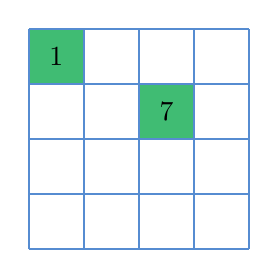
\begin{tikzpicture}[scale=0.7]
		
		\fill[diendantoanhoc] (0,3) rectangle (1,4);
		\fill[diendantoanhoc] (2,2) rectangle (3,3);
		\draw (0.5,3.5) node {$\color{black}1$};
		\draw (2.5,2.5) node {$\color{black}7$};
		
		\draw[step=1.0,cackithi,thick] (0,0) grid (4,4);
	\end{tikzpicture}
	\quad
	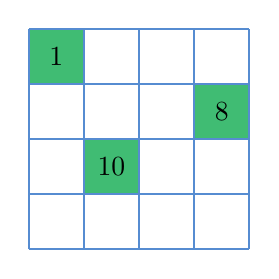
\begin{tikzpicture}[scale=0.7]
		
		\fill[diendantoanhoc] (0,3) rectangle (1,4);
		\fill[diendantoanhoc] (1,1) rectangle (2,2);
		\fill[diendantoanhoc] (3,2) rectangle (4,3);
		\draw (0.5,3.5) node {$\color{black}1$};
		\draw (1.5,1.5) node {$\color{black}10$};
		\draw (3.5,2.5) node {$\color{black}8$};
		
		\draw[step=1.0,cackithi,thick] (0,0) grid (4,4);
	\end{tikzpicture}
	
	\textit{\color{toancuabi}Hình $1.$ \hspace*{60pt}  Hình $2.$}
\end{center}
Do đó, trên hàng đầu tiên, màu xanh chỉ có thể tô ở ô số $2$ hoặc số $3$.
\vskip 0.1cm 
Ta sẽ xét cho trường hợp tô ở ô số $2$, trường hợp ô số $3$ được thực hiện tương tự.
Khi màu xanh đầu được tô ở ô số $2$, thì hàng $2$ sẽ là ô số $8$, hàng $3$ là ô số $9$ và hàng $4$ là ô số $15$.  (Hình $3$)
\begin{center}
	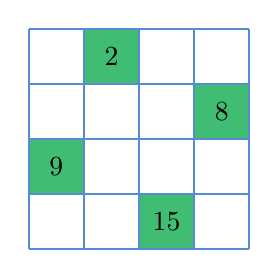
\begin{tikzpicture}[scale=0.7]
		
		\fill[diendantoanhoc] (0,1) rectangle (1,2);
		\fill[diendantoanhoc] (2,0) rectangle (3,1);
		\fill[diendantoanhoc] (3,2) rectangle (4,3);
		\fill[diendantoanhoc] (1,3) rectangle (2,4);
		\draw (0.5,1.5) node {$\color{black}9$};
		\draw (2.5,0.5) node {$\color{black}15$};
		\draw (3.5,2.5) node {$\color{black}8$};
		\draw (1.5,3.5) node {$\color{black}2$};
		
		\draw[step=1.0,cackithi,thick] (0,0) grid (4,4);
	\end{tikzpicture}
	
	\textit{\color{toancuabi}\small Hình $3$.}
\end{center}
Tiếp đến, Mít Đặc tô $4$ màu còn lại. Do mỗi màu không thể cùng trên đường chéo, nên mỗi ô vuông ở mỗi góc tương ứng với một màu. Chẳng hạn, $4$ màu trên được tô trên $4$ góc như sau, các trường hợp khác được xét tương tự.
\begin{figure}[H]
	\centering
	\vspace*{-5pt}
	\captionsetup{labelformat= empty, justification=centering}
	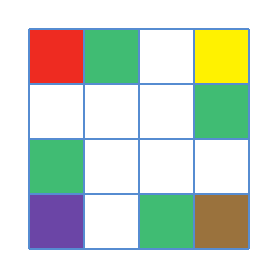
\begin{tikzpicture}[scale=0.7]
		\fill[diendantoanhoc] (0,1) rectangle (1,2);
		\fill[diendantoanhoc] (2,0) rectangle (3,1);
		\fill[diendantoanhoc] (3,2) rectangle (4,3);
		\fill[diendantoanhoc] (1,3) rectangle (2,4);
		\fill[gocco] (0,0) rectangle (1,1);
		\fill[toanhocdoisong] (0,3) rectangle (1,4);
		\fill[yellow] (3,3) rectangle (4,4);
		\fill[lichsutoanhoc] (3,0) rectangle (4,1);
		
		\draw[step=1.0,cackithi,thick] (0,0) grid (4,4);
	\end{tikzpicture}
	\quad
	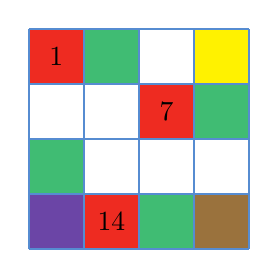
\begin{tikzpicture}[scale=0.7]
		\fill[diendantoanhoc] (0,1) rectangle (1,2);
		\fill[diendantoanhoc] (2,0) rectangle (3,1);
		\fill[diendantoanhoc] (3,2) rectangle (4,3);
		\fill[diendantoanhoc] (1,3) rectangle (2,4);
		\fill[gocco] (0,0) rectangle (1,1);
		\fill[toanhocdoisong] (2,2) rectangle (3,3);
		\fill[toanhocdoisong] (0,3) rectangle (1,4);
		\fill[toanhocdoisong] (1,0) rectangle (2,1);
		\fill[yellow] (3,3) rectangle (4,4);
		\fill[lichsutoanhoc] (3,0) rectangle (4,1);
		\draw (0.5,3.5) node {$\color{black}1$};
		\draw (2.5,2.5) node {$\color{black}7$};
		\draw (1.5,0.5) node {$\color{black}14$};
		
		\draw[step=1.0,cackithi,thick] (0,0) grid (4,4);
	\end{tikzpicture}
	\quad
	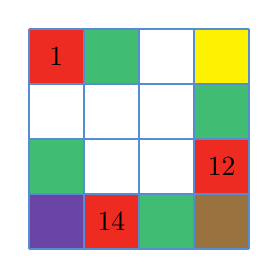
\begin{tikzpicture}[scale=0.7]
		\fill[diendantoanhoc] (0,1) rectangle (1,2);
		\fill[diendantoanhoc] (2,0) rectangle (3,1);
		\fill[diendantoanhoc] (3,2) rectangle (4,3);
		\fill[diendantoanhoc] (1,3) rectangle (2,4);
		\fill[gocco] (0,0) rectangle (1,1);
		\fill[toanhocdoisong] (1,0) rectangle (2,1);
		\fill[toanhocdoisong] (0,3) rectangle (1,4);
		\fill[toanhocdoisong] (3,1) rectangle (4,2);
		\fill[yellow] (3,3) rectangle (4,4);
		\fill[lichsutoanhoc] (3,0) rectangle (4,1);
		\draw (0.5,3.5) node {$\color{black}1$};
		\draw (3.5,1.5) node {$\color{black}12$};
		\draw (1.5,0.5) node {$\color{black}14$};
		
		\draw[step=1.0,cackithi,thick] (0,0) grid (4,4);
	\end{tikzpicture}
\caption{\small\textit{\color{toancuabi}Hình $4$ \hspace*{55pt} Hình $5$ \hspace*{55pt}Hình $6$}}
\end{figure}
Tiếp theo, bạn Mít Đặc chọn một màu và tô tiếp, chẳng hạn màu đỏ. Vị trí của $3$ ô màu đỏ có thể là $1$, $7$, $14$ hoặc $1$, $12$, $14$.Tuy nhiên, nếu màu đỏ tô ở các ô $1$, $12$, $14$ (Hình $6$) thì màu tím không có cách nào tô thỏa mãn. Do đó, màu đỏ sẽ được tô ở các ô: $1$, $7$, $14$. (Hình $5$)
\vskip 0.1cm
Từ đó, màu vàng sẽ được tô ở các ô: $4$, $5$, $11$, màu tím được tô ở các ô: $6$, $12$, $13$ và cuối cùng các ô còn lại là cho màu nâu: $3$, $10$, $16$. (Hình $7$)
\begin{center}
	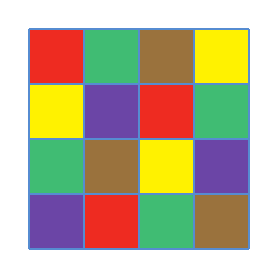
\begin{tikzpicture}[scale=0.7]
		\fill[diendantoanhoc] (0,1) rectangle (1,2);
		\fill[diendantoanhoc] (2,0) rectangle (3,1);
		\fill[diendantoanhoc] (3,2) rectangle (4,3);
		\fill[diendantoanhoc] (1,3) rectangle (2,4);
		\fill[gocco] (1,2) rectangle (2,3);
		\fill[gocco] (3,1) rectangle (4,2);
		\fill[gocco] (0,0) rectangle (1,1);
		\fill[toanhocdoisong] (2,2) rectangle (3,3);
		\fill[toanhocdoisong] (0,3) rectangle (1,4);
		\fill[toanhocdoisong] (1,0) rectangle (2,1);
		\fill[yellow] (3,3) rectangle (4,4);
		\fill[yellow] (0,2) rectangle (1,3);
		\fill[yellow] (2,1) rectangle (3,2);
		\fill[lichsutoanhoc] (3,0) rectangle (4,1);
		\fill[lichsutoanhoc] (1,1) rectangle (2,2);
		\fill[lichsutoanhoc] (2,3) rectangle (3,4);
		
		\draw[step=1.0,cackithi,thick] (0,0) grid (4,4);
	\end{tikzpicture}
	
	\textit{\small\color{toancuabi}Hình $7.$}
\end{center}
Như vậy, bằng cách lập luận như trên, bạn Mít Đặc đã thực hiện được yêu cầu của họa sĩ Thuốc Nước rồi đấy. Hy vọng lần này bạn ấy sẽ vẽ được những bức chân dung đẹp hơn các bạn nhỉ.
\begin{figure}[H]
	\centering
	\vspace*{-5pt}
	\captionsetup{labelformat= empty, justification=centering}
	\includegraphics[width=0.5\linewidth]{8}
	\vspace*{-15pt}
\end{figure}
Câu chuyện $5.$
\vskip 0.1cm
Nhận thấy quãng đường đi lên và đi xuống quả đồi của hai bạn là như nhau, mà vận tốc lúc xuống gấp $3$ lần vận tốc lúc lên, nên thời gian lên dốc gấp $3$ lần thời
gian xuống dốc. Tổng thời gian hai bạn đi lên và đi xuống quả đồi là $4$ tiếng, vậy lúc lên các bạn đi mất $3$ tiếng và lúc xuống các bạn đi mất $1$ tiếng.
Như vậy, quả đồi dài 6km và quãng đường các bạn phải đi là $12$km.
\vskip 0.1cm
Câu chuyện $6$.
\vskip 0.1cm
Đổi: $1 \mbox{ giờ} = 60 \mbox{ phút}$ nên: 
\vskip 0.1cm
$\bullet$ $\dfrac{3}{4} \mbox{ giờ}$ = $\dfrac{3}{4}\times 60 \mbox{ phút}= \dfrac{3\times 60}{4}  \mbox{ phút}= \dfrac{180}{4}  \mbox{ phút}= 45 \mbox{ phút}.$ 
\vskip 0.1cm
$\bullet$ $1\dfrac{1}{2} \mbox{ giờ}= \dfrac{3}{2} \mbox{ giờ} = \dfrac{3}{2}\times 60  \mbox{ phút}= \dfrac{3\times 60}{2}  \mbox{ phút}= \dfrac{180}{2}  \mbox{ phút}= 90 \mbox{ phút}.$
\vskip 0.1cm
Tổng thời gian mà các chú tí hon tập luyện là:
\begin{align*}
	25 + 45 + 90= 160 \ (\textrm{phút}).
\end{align*}
Nếu các chú bắt đầu dạy lúc $7$ giờ $40$ phút thì sau $20$ phút sẽ là $8$ giờ. Vậy, khi $8$ giờ thì còn phải luyện tập thêm
\begin{align*}
	160-20=140\ (\textrm{phút})
\end{align*}
nữa. Ta có:
\begin{align*}
	140= 2\times 60 +20
\end{align*}
nên $140$ phút $=2$ giờ và $20$ phút. Vậy, nếu các chú tí hon luyện tập $140$ phút kể từ lúc $8$ giờ thì các chú ấy sẽ kết thúc vào lúc  $10$ giờ $20$ phút.
\vskip 0.1cm
Đáp số: $10$ giờ $20$ phút.
\vskip 0.1cm
Câu chuyện $7.$
\vskip 0.1cm
Tổng số phút các chú tí hon đã đi từ lúc bay qua đám mây là:
\vskip 0.1cm
$40 + 60 + 10 + 80 + 20 = 210$ (phút)
\vskip 0.1cm
Đổi $210$ phút  $= 3$ giờ $30$ phút.
\vskip 0.1cm
Thời gian các chú tí hon bay qua đám mây là: $11$ giờ $30$ phút. Do đó, các chú tí hon còn phải đi $2$ tiếng mới đến được hòn đảo.
\vskip 0.1cm
Câu chuyện $8.$ 
\vskip 0.1cm
Lưu ý rằng một tuần dài gấp $7$ lần so với một ngày. Điều này cho thấy kết quả của tính toán của Biết Tuốt không phải là $1$ tuần cũng như không phải là $1$ ngày. Tương tự, vì một tháng dài gấp $30$, $31$ hoặc $28$, hay $29$ lần so với một ngày và trong các câu trả lời của các chú tí hon không chứa số nào trong các số trên nên kết quả tính toán của Biết Tuốt không phải là một tháng. Như vậy, kết quả tính toán của Biết Tuốt phải hoặc là $1$ giây, $1$ phút hoặc là $1$ giờ. Nếu kết quả tính toán là $1$ giây hay $1$ phút thì trong một giờ có $60$ phút, trong một ngày có $60 \times 24 = 1440$ phút và trong một tuần có $1440\times 7 = 10080$ phút, do đó sai nhiều hơn $3600$ lần so với tính toán! Như vậy, kết quả tính toán chỉ có thể là $1$ giờ. Ta hãy kiểm tra lại điều này: -- $1$ giờ $= 60$ phút. -- $1$ phút $= 60$ giây. Vì thế, $1$ giờ = $60\times 60 = 3600$ giây. -- $1$ ngày $= 24$ giờ. -- $1$ tuần $= 7$ ngày. Vì thế, $1$ tuần = $7\times 24 = 168$ giờ. -- $1$ tháng có $30$ ngày (như tháng $11$) sẽ có số giờ là $30\times 24 = 720$ giờ. Như vậy, theo tính toán của Biết Tuốt thì kinh khí cầu sẽ tới thành phố mới sau $1$ giờ.
\vskip 0.1cm
Câu chuyện $9.$
\vskip 0.1cm
Ngôi nhà có số nhà là $3$ được sơn màu vàng. Do ngôi nhà màu đỏ chỉ nằm cạnh đúng một ngôi nhà khác nên nó phải nằm ở một trong hai đầu của đoạn phố đó. Ngôi nhà màu xanh nằm cạnh ngôi nhà màu vàng và ngôi nhà màu đỏ. Thế nên thứ tự từ ngôi nhà màu đỏ tới đầu còn lại của con phố là đỏ, xanh, vàng. Như vậy, ngôi nhà màu vàng là ngôi nhà nằm chính giữa. Do đó, nhà của Đinh Ốc được sơn màu vàng.
\vskip 0.1cm
Câu chuyện $10.$
\vskip 0.1cm
Do tổng số táo của bốn bạn là $100$ và số táo của Bu Loong hái được gấp ba lần tổng số táo của ba bạn còn lại nên dễ thấy Bu Loong hai chuyển được $75$ quả táo còn tổng số táo mà $3$ bạn còn lại chuyển là $25$. 
\begin{figure}[H]
	\centering
	\vspace*{-5pt}
	\captionsetup{labelformat= empty, justification=centering}
	\includegraphics[width=1\linewidth]{9}
	\vspace*{-15pt}
\end{figure}
Do Mít Đặc chuyển được nhiều hơn $5$ quả táo nên số táo mà cậu ấy chuyển được ít nhất là $6$ quả.
\vskip 0.1cm
Nhận thấy nếu Mít Đặc chuyển được ít nhất là $7$ quả thì số táo mà Mít Đặc chuyển ít nhất là $8$ và số táo của Nhanh Nhảu ít nhất là $11$. Khi đó, tổng số táo chuyển được của ba bạn ít nhất phải là $7 + 8 + 11 = 26$ (mâu thuẫn).
\vskip 0.1cm
Vậy Mít Đặc chuyển được $6$ quả táo. 
\vskip 0.1cm
$+)$ Nếu Ngộ Nhỡ chuyển được $7$ quả táo thì khi đó Nhanh Nhảu được $10$ quả và tổng số táo của ba bạn là $23$ khác $25$. Vậy trường hợp này không xảy ra.
\vskip 0.1cm
$+)$ Nếu Ngộ Nhỡ chuyển được $8$ quả thì Nhanh Nhảu được $11$ quả và ta được đẳng thức $6+8+11= 25$.
\vskip 0.1cm
$+)$ Nếu Ngộ Nhỡ chuyển trên $8$ quả thì thấy ngay tổng số táo của ba bạn trên $25$ quả và do vậy trường hợp này cũng không xảy ra.
\vskip 0.1cm
Vậy Mít Đặc chuyển được $6$ quả táo, Ngộ Nhỡ chuyển được $8$ quả, Nước Đường chuyển được $11$ quả và Bu Loong nhờ “cơ khí hóa” chuyển được số táo nhiều nhất là $75$ quả.
\vskip 0.1cm
Câu chuyện $11.$ 
Theo lời của các cô tí hon, lều của các cô còn có thể nhận số lượng khách là:
\begin{align*}
	18 : 2 = 9 \,\,(\text{người}).
\end{align*}
Mà lúc đó, lều đã chứa $3/4$ số lượng khách so với khả năng của mình.
Như vậy, số khách mà lều còn có thể nhận so với khả năng của mình là:
\begin{align*}
	1- 3 /4 = 1/ 4 .
\end{align*}
Ta có sơ đồ về số lượng khách đã có và số lượng khách mà lều có thể nhận:
\begin{center}
	\begin{tikzpicture}[scale =0.6]
		\definecolor{upmaroon}{rgb}{0.48, 0.07, 0.07}
		\draw[very thick,color=toanhocdoisong] (0,0)--(9,0);
		\draw[very thick, dash dot,color=diendantoanhoc] (9,0)--(12,0);
		\draw[thick,color=toancuabi] (0, -0.1)--(0, 0.1) (3,-0.1)--(3,0.1) (6,-0.1)--(6,0.1) (9,-0.1)--(9,0.1) (12,-0.1)--(12,0.1);
		\node at (3,-0.8) {\color{toanhocdoisong}{Lượng khách}};
		\node at (3.2,-1.8) {\color{toanhocdoisong}{đã có}};
		\node at (9,-0.8) {\color{diendantoanhoc}{Lượng khách lều}};
		\node at (9,-1.8) {\color{diendantoanhoc}{có thể nhận}};
	\end{tikzpicture}
\end{center}
Như vậy, tổng số lượng khách mà lều có thể nhận là:
\begin{align*}
	9\times4 = 36 \,\,(\text{người}). 
\end{align*}
Ta có sơ đồ sau:
\begin{center}
	\begin{tikzpicture}[scale=0.6]
		\definecolor{upmaroon}{rgb}{0.48, 0.07, 0.07}
		\draw[very thick,color=timhieukhoahoc] (0,0)--(8,0);
		\draw[very thick,color=duongvaotoanhoc] (8,0)--(12,0);
		\draw[thick,color=toancuabi] (0,-0.1)--(0,0.1) (4,-0.1)--(4,0.1) (8,-0.1)--(8,0.1) (12,-0.1)--(12, 0.1);
		\node at (4,-0.8) {\color{timhieukhoahoc}{Sức chứa của}};
		\node at (4.1,-1.8) {\color{timhieukhoahoc}{lều lớn}};
		\node at (10,-0.8) {\color{duongvaotoanhoc}{Sức chứa của}};
		\node at (10,-1.8) {\color{duongvaotoanhoc}{lều nhỏ}};
	\end{tikzpicture}
\end{center}
Từ đó suy ra số lượng khách mà lều nhỏ có thể chứa là: $36 : 3 = 12$ (người).
\vskip 0.1cm
Câu chuyện $12.$
\vskip 0.1cm
Đinh Dép bắt đầu sơn từ điểm cách mép trái là $2$ mét và kết thúc tại vị trí cách mép trái:
\begin{align*}
	2+9 = 11 (m).
\end{align*}
Ta biết rằng Lặng Lẽ kết thúc khi cách mép trái của hàng rào là $4$ mét và thùng sơn của Lặng Lẽ sơn được $10$ mét hàng rào. Vì thế nên Lặng Lẽ đã bắt đầu sơn từ vị trí cách mép trái của hàng rào là:
\begin{align*}
	4+10 = 14 \,\,(m).
\end{align*}
Như vậy, có tất cả $2$ đoạn của hàng rào được sơn đúng một lớp sơn là:
\vskip 0.1cm
$1.$ đoạn hàng rào từ vị trí cách mép trái $2$ mét cho tới vị trí cách mép trái $4$ mét. Đây là đoạn hàng rào chỉ được sơn bởi Đinh Dép. Độ dài của đoạn này là
\begin{align*}
	4-2 = 2 \,\,(m).
\end{align*}
$2.$ đoạn hàng rào từ vị trí cách mép trái $11$ mét cho tới vị trí cách mép trái $14$ mét. Đây là đoạn hàng rào chỉ được sơn bởi Lặng Lẽ. Độ dài của đoạn này là:
\begin{align*}
	14-11 = 3 \,\,(m). 
\end{align*}
Như vậy, tổng độ dài của phần hàng rào được sơn bởi đúng một lớp sơn là:
\begin{align*}
	2+3 = 5 \,\,(m).
\end{align*}
\begin{center}
	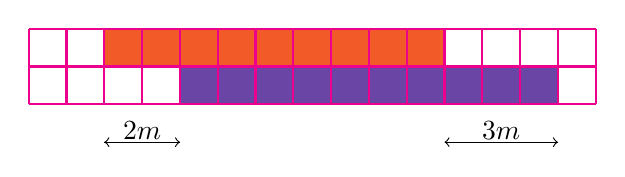
\begin{tikzpicture}[scale =0.48]
		\fill[gocco] (4,0) rectangle (14,1);
		\fill[duongvaotoanhoc] (2,2) rectangle (11,1);
		%\draw[thick,color=toancuabi] (2,1) grid (9,1);
		%\fill[timhieukhoahoc] (2,1) rectangle (9,1);
		\draw[thick,color=toancuabi] (0,0) grid (15,2);
		%\fill[yellow] (4,0) rectangle (10,1);
		\draw [->] (4,-1)--(2,-1);
		\draw [->] (2,-1)--(4,-1);
		\node at (3,-0.7){$2m$}; 
		\draw [->] (11,-1)--(14,-1);
		\draw [->] (14,-1)--(11,-1);
		\node at (12.5,-0.7){$3m$}; 
	\end{tikzpicture}
\end{center}
Câu chuyện $13.$ 
\vskip 0.1cm
Do bánh gato giá $13$ đồng nên số bánh gato Bạch Tuyết mua sẽ ít hơn hay bằng $7$. Do $1$ đồng được hai xu kem nên số bánh xu kem là số chẵn. Khi đó có thể xảy ra các trường hợp sau
\begin{table}[H]
	\centering
	\renewcommand{\arraystretch}{1.3}
	\resizebox{\columnwidth}{!}{\begin{tabular}{|l|c|c|c|c|c|c|c|}
		\hline
		Số bánh gato & $1$ &$2$& $3$&$4$&$5$&$6$&$7$\\
		\hline
		Số bánh xu kem & $98$ &$98$& $97$&$96$&$95$&$94$&$93$\\
		\hline
		Số tiền mua bánh vòng & Loại &$26$ &Loại& $52$&Loại&$72$&Loại\\
		\hline
		Số tiền mua xu kem & Loại &$49$ &Loại& $48$&Loại&$47$&Loại\\
		\hline
		Tổng số tiền &  &$75$ && $100$&&$119$&\\
		\hline
	\end{tabular}}
\end{table}
Vậy Bạch Tuyết có thể mua $4$ cái bánh gato và $96$ cái bánh xu kem.
\vskip 0.1cm
Câu chuyện $14.$
\vskip 0.1cm
Nếu Thuốc Viên không ra khỏi bệnh viện để đến nhà Mít Đặc sớm hơn $8$ phút, thì trong trường hợp nếu cậu ta quay trở lại bệnh viện để lấy quần áo rồi tới nhà Mít Đặc, Thuốc Viên sẽ muộn không phải chỉ $10$ phút mà tận $18$ phút. Đó cũng là số thời gian cậu ta bị mất khi đi $2$ lần quãng đường từ bệnh viện tới chỗ nhớ ra quên chưa thay quần áo bệnh viện. Vì vậy số thời gian cậu ta đi một lần từ bệnh viện tới chỗ sực nhớ là quên thay áo là $18 : 2 = 9$ phút, có nghĩa là cậu ta đã đi được $9/20$ quãng đường.
\vskip 0.1cm
$15.$
Để thuận tiện trong việc đếm số quân, Mít Đặt có thể xếp các quân domino theo hàng, sao cho ô vuông đầu có số chấm vượt quá số chấm của ô vuông sau. Khi đó, toàn bộ quân domino của bộ mới có thể liệt kê theo bảng sau.
\begin{table}[H]
	\centering
	\renewcommand{\arraystretch}{1.3}
	\begin{tabular}{|m{1.5cm}|m{1.5cm}|m{1.5cm}|m{1.5cm}|m{1.5cm}|}
		\hline
		$\color{toanhocdoisong}0-0$ & $0-1$& $0-2$ & $\cdots$ &$0-12$\\
		\hline
		 & $\color{toanhocdoisong}1-1$& $1-2$&$\cdots$& $1-12$\\
		 \hline
		 & & $\color{toanhocdoisong}2-2$&$\cdots$& $2-12$\\
		 \hline
		 & & &$\vdots$& $\vdots$\\
		 \hline
		 & & & & $\color{toanhocdoisong}12-12$\\
		 \hline
	\end{tabular}
\end{table}
Ta thấy,
\vskip 0.1cm
-- Có $13$ quân domino có ô vuông đầu là $0$;
\vskip 0.1cm
-- Có $12$ quân domino có ô vuông đầu là $1$;
\vskip 0.1cm
-- Có $11$ quân domino có ô vuông đầu là $2$;
\vskip 0.1cm
-- $\ldots$
\vskip 0.1cm
Tiếp tục đếm như trên, cuối cùng có $1$ quân domino có ô vuông đầu là $12$.
\vskip 0.1cm
Như vậy, tổng số quân trong bộ domino mới là:
\begin{align*}
	13 + 12 + \ldots + 1 = \frac{14\times13}{2}=91.
\end{align*}
Câu chuyện $16.$
\vskip 0.1cm
Sau lần Nhanh Nhảu lấy $8$ chiếc kẹo cuối cùng, trong hộp có đúng $8$ chiếc, gấp đôi số kẹo sau lần trao đổi thứ hai. Vì vậy sau lần trao đổi kẹo thứ hai, trong hộp có $8:2=4$ (chiếc kẹo). Trước khi Nhanh Nhau lấy mất $8$ chiếc, số kẹo trong hộp phải là $4+8 = 12$ (chiếc). Vậy sau lần
thứ nhất trong hộp có $12:2 = 6$ chiếc. Trước khi Nhanh Nhảu xin $8$ chiếc ở lần trao đổi thứ nhất, trong hộp có $6+8=14$ (chiếc kẹo). Vậy ban đầu Mít Đặc có $14:2=7$ (chiếc kẹo).
\vskip 0.1cm
Số kẹo cho và nhận giữa Mít Đặc và Nhanh Nhảu được tóm tắt trong bảng sau.
\begin{table}[H]
	\centering
	\renewcommand{\arraystretch}{1.3}
	\resizebox{\columnwidth}{!}{\begin{tabular}{|c|c|c|c|}
		\hline
		Lần&	\makecell{Kẹo Mít Đặc \\trước khi được cho}&	\makecell{Kẹo Mít Đặc\\ sau khi được cho}&	\makecell{Số kẹo\\ Nhanh Nhảu lấy}\\
		\hline
		Lần $1$&	$7$&	$14$&	$8$\\
		\hline
		Lần $2$&	$6$&	$12$&	$8$\\
		\hline
		Lần $3$&	$4$&	$8$&	$8$\\
		\hline
		Cuối cùng&	$0$ &	&\\
		\hline		
	\end{tabular}}
\end{table}
Câu chuyện $17.$
\vskip 0.1cm
Gọi $a$ là số thời gian tính theo phút từ lúc hai thi sĩ khởi hành tới lúc gặp nhau. Vận tốc của Kèn Đồng là $g$, vận tốc của Hoa Dại là $d$, khi đó ta có quãng đường từ nhà Hoa Dại tới điểm gặp là da, quãng đường từ nhà Kèn Đồng tới điểm gặp là ga. Sau khi gặp, Kèn Đồng đi tiếp $1.g$ còn Hoa Dại đi tiếp $4d$.
\begin{figure}[H]
	\centering
	\vspace*{-5pt}
	\captionsetup{labelformat= empty, justification=centering}
	\includegraphics[width=1\linewidth]{13}
	\vspace*{-15pt}
\end{figure}
So sánh quãng đường từ lúc khởi hành đến lúc gặp theo hai cách, ta có $1g = da$ và $4d=ga$.
\vskip 0.1cm
Nhân hai vế của hai đẳng thức trên với nhau ta có $4dg= a.a.gd$. Giản ước cho $gd$ ta có  $a.a=4$. Số $a$ duy nhất thỏa mãn là $a=2$. Vậy Hoa Dại đi mất $2+4 = 6$ phút, còn Kèn Đồng đi mất $2+1 = 3$ phút.
\vskip 0.1cm
Câu chuyện $18.$ 
\vskip 0.1cm
Gọi số cô tí hon là $a$, số túi mỗi cô đã may được là $b$. Khi đó, tổng số túi các cô tí hon đã làm được là $ab$. Mỗi cô tí hon đã tặng a túi cho mỗi chú tí hon, vì vậy có tất cả a×a số túi được tặng đi. Vì thế, cuối cùng các cô đã mang đến $ab - a\times a$ túi đến nhà Bạch Tuyết.
\vskip 0.1cm
Ta có $ab - a\times a =33$, hay là $a(b-a) = 33$. Do đó, a là ước số của $33$. Theo đề bài, do $b - a > 1$ và $a>1$ nên a phải khác $1$ và $33$, vì thế $a=3$ hoặc $a= 11$.
\begin{table}[H]
	\centering
	\renewcommand{\arraystretch}{1.3}
	\begin{tabular}{|c|c|c|}
		\hline
		$a$ & $3$ & $11$\\
		\hline
		$a-b$& $11$ & $3$\\
		\hline
		$b$ & $14$ & $14$\\
		\hline
	\end{tabular}
\end{table}
Trong cả hai trường hợp, chúng ta thấy số túi các cô tí hon may được đều bằng $14$.
\vskip 0.1cm
Câu chuyện $19$.
\vskip 0.1cm
Theo thông tin từ bài, người đầu tiên (người số $1$) của Tròn Xoay phải là người số $14$ của Mít Đặc. Vì thế người ở vị trí cuối cùng của Tròn Xoay sẽ là người số $13$ theo cách đếm của Mít Đặc. Từ đó suy ra hiệu số của các số thứ tự của người số $94$ và người cuối cùng theo cách đếm của Tròn Xoay cũng chính là hiệu số giữa số thứ tự của người số $7$ và người số $13$  theo cách đếm của Mít Đặc. Vì thế người cuối cùng là người số: $94+ 13-7=100$ theo cách đếm của Tròn Xoay.
\begin{figure}[H]
	\centering
	\vspace*{-5pt}
	\captionsetup{labelformat= empty, justification=centering}
	\includegraphics[width=0.45\linewidth]{15}
	\vspace*{-15pt}
\end{figure}
Vậy vòng tròn trong buổi vũ hội có $100$ cô chú tí hon.
\vskip 0.1cm
Câu chuyện $20.$ 
\vskip 0.1cm
Theo hình vẽ bên, ta thấy số ngày dự tính làm kinh khí cầu bằng số chú tí hon tham gia vào làm nhân với mỗi ngày làm của mỗi chú.
Số chú tí hon tham gia vào làm kinh khí cầu là: $20 : 2 = 10$ (người)
\vskip 0.1cm
Số ngày cần thiết để làm kinh khí cầu là: $10 \times 4 = 40$ (ngày)
\begin{figure}[H]
	\centering
	\vspace*{-5pt}
	\captionsetup{labelformat= empty, justification=centering}
	\includegraphics[width=0.85\linewidth]{16}
	\vspace*{-15pt}
\end{figure}
\newpage
\begin{center}
	{\color{toanhocdoisong}{\textbf{\color{toancuabi}ĐÁP ÁN PHẦN III SUY LUẬN CÙNG BI}}}
\end{center}
\begin{center}
	\textbf{\color{toancuabi}Đáp án các bài toán trong bài\\ Sumi và những chiếc lá sắc màu}
\end{center}
Câu đố $4$. % thực ra là câu 5

Jenny có thể trả lời ngay mình đội mũ màu gì chứng tỏ Sumi và Julia cùng đội mũ xanh. Sumi thấy bạn trả lời quả quyết như vậy thì chắc chắn mình đội mũ xanh rồi. Sumi nói đúng phải không các em?
\vskip 0.1cm
Câu đố $5$. % thực ra là câu 4  , ở bài viết cần hoán đổi hai câu

Julia suy luận từ hai câu trả lời của hai anh chị Sumi và Jenny và trả lời bố là mình đội mũ màu đỏ. Thật vậy, Julia sẽ nghĩ như thế này: nếu mình đội mũ màu xanh và:
\vskip 0.1cm
$1.$ nếu một trong hai anh chị đội mũ xanh chẳng hạn là anh Sumi thì lập tức chị Jenny sẽ biết là Jenny đội mũ đỏ vì chỉ có hai chiếc mũ xanh.
\vskip 0.1cm
$2.$  nếu cả hai anh chị đội mũ đỏ. Khi đó, Sumi nhìn thấy một mũ xanh và một mũ đỏ sẽ không biết mình đội mũ gì. Jenny đã thấy Julia đội mũ xanh và biết Sumi không kết luận được mũ của chính mình nên Julia biết mũ của mình màu đỏ. Vậy Julia biết chính xác màu mũ của chị.
\vskip 0.1cm
Nhưng cả hai anh chị không biết màu mũ của mình nên mũ của Julia phải là màu đỏ.

\newpage
\begin{center}
	\textbf{\color{toancuabi}ĐÁP ÁN CÁC BÀI TOÁN TRONG BÀI $\pmb9$ SODUKO}
\end{center}
\begin{multicols}{2}
	\begin{figure}[H]
		\centering
		\vspace*{-5pt}
		\captionsetup{labelformat= empty, justification=centering}
		\includegraphics[width=0.9\linewidth]{sudoku1}
		\caption{\small{Bài tập $1$}}
		\vspace*{-10pt}
	\end{figure}
	\begin{figure}[H]
		\centering
		\vspace*{-5pt}
		\captionsetup{labelformat= empty, justification=centering}
		\includegraphics[width=0.9\linewidth]{sudoku2}
		\caption{\small{Bài tập $2$}}
		\vspace*{-10pt}
	\end{figure}
	\begin{figure}[H]
		\centering
		\vspace*{-5pt}
		\captionsetup{labelformat= empty, justification=centering}
		\includegraphics[width=0.9\linewidth]{sudoku3}
		\caption{\small{Bài tập $3$}}
		\vspace*{-10pt}
	\end{figure}
	\begin{figure}[H]
		\centering
		\vspace*{-5pt}
		\captionsetup{labelformat= empty, justification=centering}
		\includegraphics[width=0.9\linewidth]{sudoku4}
		\caption{\small{Bài tập $4$}}
		\vspace*{-10pt}
	\end{figure}
	\begin{figure}[H]
		\centering
		\vspace*{-5pt}
		\captionsetup{labelformat= empty, justification=centering}
		\includegraphics[width=0.9\linewidth]{sudoku5}
		\caption{\small{Bài tập $5$}}
		\vspace*{-10pt}
	\end{figure}
	\begin{figure}[H]
		\centering
		\vspace*{-5pt}
		\captionsetup{labelformat= empty, justification=centering}
		\includegraphics[width=0.9\linewidth]{sudoku6}
		\caption{\small{Bài tập $6$}}
		\vspace*{-10pt}
	\end{figure}
\end{multicols}
\newpage
\begin{center}
	\textbf{\color{toancuabi}ĐÁP ÁN CÁC BÀI TOÁN TRONG BÀI $\pmb{10}$ GẶP GỠ CUỐI NĂM: TRÒ CHUYỆN VỚI \\
		THANH TRA LÊ KÍNH}
\end{center}
\textbf{\color{toancuabi}Thổ ngữ châu Phi} 
\vskip 0.1cm
Trong ngôn ngữ địa phương, hai câu đầu tiên  ``KAF NAVCKI ROI" và "KIR ROI PALT" có chung từ ``ROI". Trong tiếng Việt, như thanh tra Lê Kính nói, các câu trên tương ứng với ``Lấy ba chiếc đi" và ``Hãy cất ba đồng xu" thì từ ``ba" là chung. Như vậy, nhiều khả năng là ``ROI" tương ứng với ``ba".
\vskip 0.1cm
Tương tự, nếu ta so sánh hai câu cuối ``KIR ROI PALT" và \linebreak ``INOTI KAF KIR" thì ta nhận thấy chúng có chung từ ``KIR". Trong tiếng Việt, các câu này có nghĩa là ``Hãy cất ba đồng xu" và ``Lấy mấy đồng xu cẩn thận nhé" và chúng có chung từ ``đồng xu". Do đó, nhiều khả năng là ``KIR" có nghĩa là ``đồng xu". 
\vskip 0.1cm
Cũng như vậy, nếu ta so sánh câu đầu tiên và câu cuối cùng, ``KAF NAVCKI ROI" và ``INOTI KAF KIR", thì chúng có chung từ ``KAF".  Trong tiếng Việt, chúng có nghĩa là ``Lấy ba chiếc đi" và ``Lấy mấy đồng xu ra cẩn thận nhé", và có chung từ ``Lấy". Như vậy, từ ``KAF" có nghĩa là ``Lấy".
\vskip 0.1cm
Bây giờ, trong câu đầu tiên, ``KAF NAVCKI ROI" có nghĩa là ``Lấy ba chiếc đi" và ta biết ``KAF" nghĩa là ``Lấy" còn ``ROI" nghĩa là ``ba" nên ``NAVCKI" nghĩa là ``(mấy) chiếc bánh". Trong câu thứ hai, ``KIR ROI PALT" có nghĩa là ``Hãy cất ba đồng xu", ta biết ``KIR" nghĩa là ``đồng xu", ``ROI" nghĩa là ``ba" nên ``PAL" nghĩa là ``Hãy cất". Trong câu cuối cùng, ``INOTI KAF KIR" có nghĩa là ``Lấy mấy đồng xu ra cẩn thận nhé" ta biết rằng ``KAF" có nghĩa là ``Lấy", ``KIR" có nghĩa là ``đồng xu" nên ``INOTI" có nghĩa là ``cẩn thận (nhé)".
\vskip 0.1cm
Như vậy, để nói ``\textbf{\color{toancuabi}Hãy cất mấy chiếc  bánh cẩn thận nhé}" ta chỉ cần nói ``\textbf{\color{toancuabi}PAL NAVCKI INOTI}".

\vskip 0.1cm
\textcolor{timhieukhoahoc}{\textbf{\color{toancuabi}Du hành trên đại dương}}
\vskip 0.1cm
Các em hãy quan sát lá cờ Nhật Bản nhé. Lá cờ này không thể treo ngược được vì nó hoàn toàn đối xứng khi quay luật từ trên xuống dưới. Vậy Quản lý thiết bị $1$ đã nói dối và anh ta là kẻ trộm.
\vskip 0.1cm
\textbf{\color{toancuabi}\color{toancuabi} Thử thách sống còn}
\vskip 0.1cm
Việc Xuân Phong bị bịt mắt và giam vào phòng tối cho ta thấy anh ta không thể xác  định được viên thuốc nào màu đỏ và viên nào màu xanh. Nhưng bọn cướp cho anh ta chọn thuốc, có nghĩa là hai tay của Xuân Phong không bị trói. Và với hai tay được tự do như thế, Phong có thể chia đôi mỗi viên thuốc ra, cất riêng một nửa vào một nơi, và sau đó uống tất cả các nửa viên thuốc đã chia đôi mà không bị cất đi. Xuân Phong giờ có đúng $1$ viên đỏ và $1$ viên xanh để có đủ sức phá khóa và khống chế bọn cướp. Các em nhớ là cách này chỉ áp dụng được với các viên thuốc, không phải đối với viên nang (con nhộng) nhé. Và Xuân Phong là thám tử nên chắc cũng vô cùng khéo tay để bẻ đôi chính xác mỗi một viên ra để đảm bảo liều lượng.

\vskip 0.1cm
\textbf{\color{toancuabi}\color{toancuabi}Chiếc mũ kỷ niệm} 
\vskip 0.1cm
Hai học trò đứng đầu hàng cùng đội mũ có cùng màu, đó là cách duy nhất mà tất cả ai cũng có thể đoán đúng.
\vskip 0.1cm
Thật vậy, ta gọi $3$ màu là $A$, $B$ và $C$. Thám tử Xuân Phong xếp chiếc mũ theo thứ tự từ hàng dưới lên hàng trên là $ABCC$. Học trò ở cuối hàng nhìn thấy $BCC$. Và do đó cậu ta biết ngay mình đội mũ màu $A$, và nói to lên “$A$”.
\vskip 0.1cm
Học trò tiếp theo nhìn thấy $CC$ và nghe học trò cuối hàng nói “$A$” nên cũng biết mình đội mũ màu $B$. Cậu ta trả lời ngay là “$B$”.
\vskip 0.1cm
Học trò thứ ba nghe câu trả lời của hai học trò vừa xong, biết họ đội các mũ khác màu nhau và nhìn thấy người đứng trước mình là $C$ nên biết ngay mình đội chiếc mũ cùng màu $C$. Cậu ta sẽ trả lời được “$C$”.
\vskip 0.1cm
Học  trò đầu hàng  thì chả cần phải suy nghĩ gì nữa cũng biết được mình đội mũ $C$. Vậy là Xuân Phong đã trao được món quà động viên quý báu cho $4$ trò yêu của mình như vậy.
\vskip 0.1cm
\textbf{\color{toancuabi}\color{toancuabi}Ba chiếc hộp và cô thư ký}
\vskip 0.1cm
Lê Kính sẽ nhặt một bức thư trong hòm thư “Hòm thư chưa phân loại, lẫn cả thư gửi Xuân Phong và Lê Kính”. Nếu thư này đề người nhận là Xuân Phong, thì do cả $3$ hòm thư đều ghi sai nhãn, toàn bộ thư trong hòm đều gửi cho thám tử Phong. Vì thế nhãn đúng của hòm này là “Hòm thư riêng của Xuân Phong”.
\vskip 0.1cm
Vì thế hòm đã dán nhãn “Hòm thư riêng của Lê Kính” thực ra phải dán lại nhãn là “Hòm thư chưa phân loại, lẫn cả thư gửi Xuân Phong và Lê Kính”.
\vskip 0.1cm
Và do đó hòm thư đã được dán nhãn là “Hòm thư riêng của Xuân Phong” phải là “Hòm thư riêng của Lê Kính”.
\vskip 0.1cm

\textbf{\color{toancuabi}\color{toancuabi}Vị thám tử ẩn danh}
\vskip 0.1cm
Chúng ta sẽ phác thảo ra chiếc bàn vuông để dễ tưởng tượng và thử xác định nghề nghiệp của từng người thông qua $4$ thông tin trên nhé. 
\begin{center}
	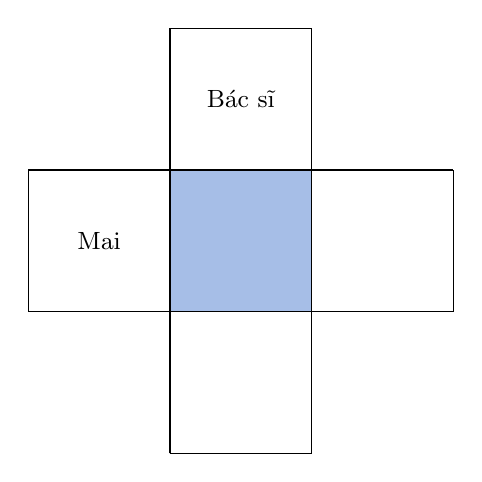
\begin{tikzpicture}[scale=1.8,font=\small]
		\fill[color=cackithi!50] (0,1) rectangle (1,2);
		\draw[thin] (0,0) grid (1,3);
		\node at (0.5,2.5) {Bác sĩ};
		\node at (-0.5,1.5) {Mai};
		\draw[thin] (-1,1) grid (2,2);
	\end{tikzpicture}
\end{center}
Theo thông tin $2$:  Anh Trọng không thể ngồi bên tay phải cô Mai vì khi đó ngồi đối diện anh ta là Bác sỹ chứ không phải Thẩm phán. Vì vậy Trọng có thể ngồi ở đối diện  Mai hoặc ngồi bên tay trái cô ấy.
\vskip 0.1cm
Theo thông tin $3$: Cô Trang và anh Vinh ngồi cạnh nhau, vì vậy $2$ người còn lại là Mai và Trọng không thể ngồi đối diện. Vì vậy ta có cách xếp sau đây với anh Trọng.
\begin{center}
	\begin{tikzpicture}[scale=1.8,font=\small]
		\fill[color=cackithi!50] (0,1) rectangle (1,2);
		\draw[thin] (0,0) grid (1,3);
		\draw[thin] (-1,1) grid (2,2);
		\node at (0.5,2.7) {Bác sĩ};
		\node at (0.5,2.3) {Trọng};
		\node at (-0.5,1.5) {Mai};
		\node at (0.5,0.5) {Thẩm phán};
	\end{tikzpicture}
\end{center}
Thông tin $4$ có thể phát biểu lại là: phía bên tay phải một phụ nữ là một luật sư. Vì vậy, cùng với Thông tin $3$, ta xếp ngay được vị trí của anh Vinh và cô Trang ở $2$ chỗ còn lại như sau
\begin{center}
	\begin{tikzpicture}[scale=1.8,font=\small]
		\fill[color=cackithi!50] (0,1) rectangle (1,2);
		\draw[thin] (0,0) grid (1,3);
		\draw[thin] (-1,1) grid (2,2);
		\node at (0.5,2.7) {Bác sĩ};
		\node at (0.5,2.3) {Trọng};
		\node at (-0.5,1.5) {Mai};
		\node at (0.5,0.7) {Thẩm phán};
		\node at (0.5,0.3) {Trang};
		\node at (1.5,1.7) {Vinh};
		\node at (1.5,1.3) {Luật sư};
	\end{tikzpicture}
\end{center}
Và chúng ta giờ đều đã biết rõ cô Mai chính là vị Thám tử tư bí mật rồi, đúng không các em.

%=================

%=================
\newpage
\begin{center}
	\textbf{\color{toancuabi}ĐÁP ÁN CÁC BÀI TOÁN TRONG PHẦN IV}
\end{center}
%=================
\begin{center}
	\textbf{\color{toancuabi}Đáp án các bài toán trong Bài $\pmb{12}$ Học làm thám tử}
\end{center}
\textbf{\color{toancuabi}Bài tập $\pmb1$:} Tay trái của Bi chỉ vào hướng Bắc, tay phải chỉ vào hướng Nam.

\textbf{\color{toancuabi}Bài tập $\pmb2$:} Ta xác định được hướng $12$ giờ như minh hoạ trong hình vẽ sau.
 \begin{figure}[H]
	\centering
	\vspace*{-5pt}
	\captionsetup{labelformat= empty, justification=centering}
	\includegraphics[width=0.45\linewidth]{bando}
	\vspace*{-5pt}
\end{figure}
 Như vậy ở hướng $11$ giờ ta có Quảng trường Đông Kinh Nghĩa Thục, hướng $1$ giờ là Nhà hát Múa rối Thăng Long. Còn Tháp Rùa ở hướng $6$ giờ.
%=================
\begin{center}
	\textbf{\color{toancuabi}Đáp án các bài toán trong Bài $\pmb{13}$ Những bài toán đếm hình tam giác}
\end{center}
\textbf{\color{toancuabi}Bài tập $\pmb1$.}
\vskip 0.1cm
Số tam giác trong Hình $4$ là: $10$ tam giác.
\vskip 0.1cm
Số tam giác trong Hình $5$ là: $21$ tam giác.
\vskip 0.1cm
\textbf{\color{toancuabi}Bài tập $\pmb2$.}
\vskip 0.1cm
Số tam giác trong Hình $9$ là: $40$ tam giác.
\vskip 0.1cm
Số tam giác trong Hình $10$ là: $31$ tam giác.
\vskip 0.1cm
\textbf{\color{toancuabi}Bài tập $\pmb3$.}
\vskip 0.1cm
Số tam giác trong Hình $15$ là: $18$ tam giác.
\vskip 0.1cm
Số tam giác trong Hình $16$ là: $28$ tam giác.
\vskip 0.1cm
Nhận xét. Số tam giác tạo bởi $n$ hình vuông dạng này là: $4\times 2\times n + 2\times (n-1)$.
\vskip 0.1cm
\textbf{\color{toancuabi}Bài tập $\pmb4$.}
\vskip 0.1cm
Số tam giác tạo thành từ tam giác có hoa văn kiểu tam giác có kích thước $6$ là: $78$ tam giác.

\newpage
\begin{center}
	\textbf{\color{toancuabi}ĐÁP ÁN ĐỐ VUI}
\end{center}

%Do_vui_Pi6_2021
\textbf{\color{toancuabi}Đố vui} $\color{toancuabi}\pmb{1.}$
Mỗi ký hiệu đều có một đường thẳng đối xứng theo phương thẳng đứng. Nếu ta loại bỏ phần bên phải của mỗi ký hiệu đối với đường thẳng này thì phần còn lại của mỗi ký hiệu có hình dạng là một chữ số. Như vậy, biểu thức bên trên trở thành $2+6=8$ và biểu thức bên dưới trở thành $1+3=?$ Vì thế câu trả lời phải là một ký hiệu mã hóa số $\color{toancuabi}4$. Đó chính là ký hiệu được cho bởi $A$).
\vskip 0.1cm
%Do_vui_Pi7_2019

\textbf{\color{toancuabi}Đố vui} $\color{toancuabi}\pmb{2.}$ Đáp án $c$.
%Do_vui_Pi6_2019
\vskip 0.1cm
\textbf{\color{toancuabi}Đố vui} $\color{toancuabi}\pmb{3.}$Đáp án là $b$).
\vskip 0.1cm
%Do_vui_Pi8_2019
\textbf{\color{toancuabi}Đố vui} $\color{toancuabi}\pmb{4.}$ Các chữ số đã biết, lần lượt theo thứ tự là $1$, $4$, $1$, $5$, $9$, $2$, $6$, $5$. Đây là các chữ số sau dấu phảy của khai triển thập phân của số $\pi$ quên thuộc. Vì thế, số cần tìm chính là số $3$ vì

$$\pi = 3, 14159265\ldots$$
Như vậy, đáp án là $c$).
\vskip 0.1cm
%Do_vui_Pi9_2019
\textbf{\color{toancuabi}Đố vui} $\color{toancuabi}\pmb{5.}$ Trả lời: mã số để mở khóa là $784$.
\vskip 0.1cm
Ta có thể luận luận như sau. Theo $b)$ thì chữ số  $3$  không xuất hiện trong mã. Như vậy, từ $c)$ thì các chữ số  $8$ và $7$ xuất hiện trong mã (nhưng nằm sai vị trí). Từ $e)$ suy ra $6$, $1$ không xuất hiện trong mã. Từ $a)$  ta thấy $4$ xuất hiện trong mã và nằm ở vị trí thứ $3$. Từ đó, mã mở khóa phải là $784$ hoặc $874$. Trong hai khả năng này, dựa vào $c)$, ta kết luận rằng mã mở khóa phải là $784$ chứ không phải là $874$.
\vskip 0.1cm

%Do_vui_Pi11_2019
\textbf{\color{toancuabi}Đố vui} $\color{toancuabi}\pmb{6.}$ Câu trả lời đúng là $B$).
\vskip 0.1cm
%Do_vui_Pi4_2020
\textbf{\color{toancuabi}Đố vui} $\color{toancuabi}\pmb{7.}$ Đáp án là $B$.
\newpage
\begin{center}
	Hội Toán học Việt Nam Tạp chí Pi\\
	Để các em thích toán\\
	(Dành cho học sinh từ lớp $2$ đến lớp $6$)\\

	------------**------------ 
\end{center}
\begin{center}
	\textbf{NHÀ XUẤT BẢN LAO ĐỘNG}\\
	\vskip 0.1cm
	Địa chỉ: Tầng $4$ -- Khu A -- Tòa nhà số $97$ Trần Quốc Toản\\
	Phường Trần Hưng Đạo, Quận Hoàn Kiếm,\\ Thành phố Hà Nội\\
	Điện thoại: $024\, 38515380$; Fax: $024\,38515381$\\
	Email: \url{info@nxblaodong.com.vn}\\
	Website: \url{www.nxblaodong.com.vn}
\end{center}
\begin{center}
	\textbf{Chi nhánh phía Nam}\\
	\vskip 0.1cm
	Số $85$ Cách mạng Tháng Tám, Quận $1$, Tp. Hồ Chí Minh\\
	Điện thoại: $028\, 38390970$; Fax: $028\, 39257205$
\end{center}
\begin{center}
	Chịu trách nhiệm xuất bản:\\
	Giám đốc -- Tổng biên tập\\
	Mai Thị Thanh Hằng\\
	Biên tập: Tạ Thị Thu Hà\\
	\vskip 0.1cm
	\vspace*{5pt}
	Trình bày:.........\\
	Bìa:.........\\
	Sửa bản in: .........
\end{center}

\begin{center}
	\textbf{Liên kết xuất bản:}\\
	\vskip 0.1cm
	Công ty TNNH MTV Hà Nội
\end{center}

In ... cuốn, khổ .......... cm, tại .....\\
Địa chỉ: ....\\
Số xác nhận ĐKXB: .....\\
Mã ISBN: .....\\
Số quyết định: ...../QĐ--NXBLĐ ngày .....\\
In xong và nộp lưu chiểu năm $2023$.
	\newpage
\end{document}


